\documentclass[11pt,headheight=35pt]{scrartcl}
\usepackage[italian]{babel}
\usepackage[sexy]{evan}

%%%%%%%%%%%%%%%%%%%%%%%%%%%%%%%%%%%%%%%%%%%%%%%%%%%%%%%%%%%%%%%%%%%%%%%%%%%%%%
%.
%
% BOOST SOFTWARE LICENSE - VERSION 1.0 - 17 AUGUST 2003
%
% Copyright (c) 2022 Evan Chen [evan at evanchen.cc]
% https://web.evanchen.cc/ || github.com/vEnhance
%  
% Available for download at:
% https://github.com/vEnhance/dotfiles/blob/main/texmf/tex/latex/evan/evan.sty
%
% Permission is hereby granted, free of charge, to any person or organization
% obtaining a copy of the software and accompanying documentation covered by
% this license (the "Software") to use, reproduce, display, distribute,
% execute, and transmit the Software, and to prepare derivative works of the
% Software, and to permit third-parties to whom the Software is furnished to
% do so, all subject to the following:
%
% The copyright notices in the Software and this entire statement, including
% the above license grant, this restriction and the following disclaimer,
% must be included in all copies of the Software, in whole or in part, and
% all derivative works of the Software, unless such copies or derivative
% works are solely in the form of machine-executable object code generated by
% a source language processor.
%
% THE SOFTWARE IS PROVIDED "AS IS", WITHOUT WARRANTY OF ANY KIND, EXPRESS OR
% IMPLIED, INCLUDING BUT NOT LIMITED TO THE WARRANTIES OF MERCHANTABILITY,
% FITNESS FOR A PARTICULAR PURPOSE, TITLE AND NON-INFRINGEMENT. IN NO EVENT
% SHALL THE COPYRIGHT HOLDERS OR ANYONE DISTRIBUTING THE SOFTWARE BE LIABLE
% FOR ANY DAMAGES OR OTHER LIABILITY, WHETHER IN CONTRACT, TORT OR OTHERWISE,
% ARISING FROM, OUT OF OR IN CONNECTION WITH THE SOFTWARE OR THE USE OR OTHER
% DEALINGS IN THE SOFTWARE.
%%%%%%%%%%%%%%%%%%%%%%%%%%%%%%%%%%%%%%%%%%%%%%%%%%%%%%%%%%%%%%%%%%%%%%%%%%%%%%

\begin{document}
\title{Elementi Di Teoria Degli Insiemi}
\subtitle{\large\normalfont\rmfamily\scshape APPUNTI DEL CORSO DI ELEMENTI DI TEORIA DEGLI INSIEMI \\ TENUTO DAL PROF. MARCELLO MAMINO}
\author{Diego Monaco \\ \textnormal{\href{d.monaco2@studenti.unipi.it}{d.monaco2@studenti.unipi.it}} \\ Università di Pisa}
\date{Anno Accademico 2022-23}
\maketitle
\begin{center}
    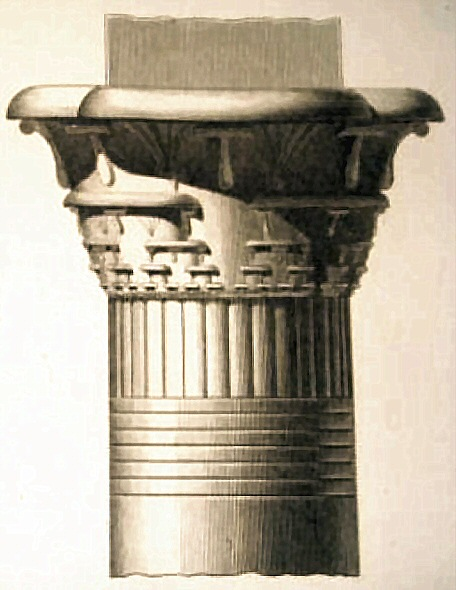
\includegraphics[scale=4.0]{immagini/Cantor-like_Column_Capital_Ile_de_Philae_Description_d'Egypte_1809.jpg}
\end{center}
\newpage

\tableofcontents
\newpage

\section*{Premessa}
Queste dispense sono la quasi esatta trascrizione in \LaTeX\,delle dispense del corso di Elementi di Teoria degli Insiemi \cite{mamino_eti_22_23}, tenuto dal prof. Marcello Mamino nell'anno accademico 2022-23 presso l'Università di Pisa.

\section*{Ringraziamenti}
Francesco Sorce, Rubens Martino, Lorenzo Picinelli, Andrea Snaidero, Alessandro Avellino, Lorenzo Bonetti.

\vfill
\begin{wrapfigure}{R}{0.2\textwidth}
	\href{https://creativecommons.org/licenses/by-nc/4.0/deed.it}{
\includegraphics[scale=0.20]{immagini/licenza.png}}
\end{wrapfigure}
Quest'opera è stata rilasciata con la licenza Creative Commons Attribuzione - Condividi allo stesso modo 4.0 Internazionale.
Per leggere una copia della licenza visita il sito web \href{http://creativecommons.org/licenses/by-sa/4.0/deed.it}{\textcolor{blue}{https://creativecommons.org/licenses/by-nc/4.0/deed.it}}.

\newpage
\section{Prologo nel XIX secolo}
La nascita della teoria degli insiemi è una storia complicata di cui so pochissimo. Però, persone che ne sanno molto più di me hanno sostenuto l'opinione che il problema seguente
abbia avuto un ruolo. Come che sia, è almeno un'introduzione possibile.

\begin{problem}
Data una serie trigonometrica:
\[ S(x) = c_0 + \sum_{i=1}^{+\infty}a_i\sin{(ix)}+b_i\cos{(ix)}
	\]
se, per ogni $x \in \RR$, sappiamo che $S(x)$ converge a 0, possiamo dire che i coefficienti $c_0,a_i,b_i$ sono tutti 0?
\end{problem}

Risolto positivamente da \href{https://it.wikipedia.org/wiki/Georg_Cantor}{\textcolor{purple}{Georg Cantor}} nel 1870.

\begin{definition}
Diciamo che $X \subseteq \RR$ è un \vocab{insieme di unicità} se, per ogni serie trigonometrica:
\[ S(x) = c_0 + \sum_{i=1}^{+\infty}a_i\sin{(ix)}+b_i\cos{(ix)}
	\]
vale la seguente implicazione:
\[ \text{$S(x)$ converge a 0 per tutti gli $x\not\in X$} \implies \text{tutti i coefficienti $c_0,a_i,b_i$ sono nulli}
	\]
\end{definition}

\begin{example}
	Per il risultato di Cantor, $\emptyset$ è di unicità.
\end{example}

\begin{problem}
	Quali sottoinsiemi di $\RR$ sono di unicità?
\end{problem}

\begin{fact}[Criterio per gli insiemi di unicità]
Dato $X \subseteq \RR$ se (ma non solo se) \textcolor{purple}{ogni funzione continua $f : \RR \to \RR$ che soddisfi:
\begin{itemize}
	\item per ogni intervallo aperto $\left]a,b\right[$ con $]a,b[ \,\cap\, X = \emptyset$, $f_{| \, ]a,b[}$ è lineare.
	\item per ogni $x \in \RR$, se $f$ ha derivate destre e sinistre in $x$, allora queste coincidono\footnote{Ovvero $f$ non ha punti angolosi.}.
\end{itemize}
è lineare}\footnote{$f(x) = \alpha x + \beta$.}, allora $X$ è di unicità.
\end{fact}

\textcolor{MidnightBlue}{D'ora in avanti diremo che un insieme rispetta le ipotesi criterio, o ha la proprietà $(\star)$, se soddisfa il fatto in \textcolor{purple}{viola}, e quindi è di unicità per il fatto sopra.}

\begin{example}
	$X = \{\ldots,a_{-2},a_{-1},a_0,a_1,a_2,\ldots\} = \{a_i | i \in \ZZ\}$ con $\ldots < a_{-2} < a_{-1} < a_0 < a_1 < a_2 <\ldots$, $\lim_{i \to +\infty} a_i = +\infty$, $\lim_{i \to -\infty} a_i = -\infty$ ha la 
	proprietà data dal \hyperref[unicità]{Fatto 1.5}, quindi è di unicità.
\end{example}

\begin{notexample}
L'intervallo $[0,1]$ o $\RR$ non hanno la proprietà espressa dall'\hyperref[unicità]{Fatto 1.5}.
\end{notexample}

\begin{notexampleb}
Per l'\vocab{insieme di Cantor} non vale il \hyperref[unicità]{Fatto 1.5}.
\end{notexampleb}

Possiamo costruire l'insieme di Cantor a partire dall'intervallo $C_0 = [0,1]$ nel seguente modo:

\begin{figure}[H]
	\centering
	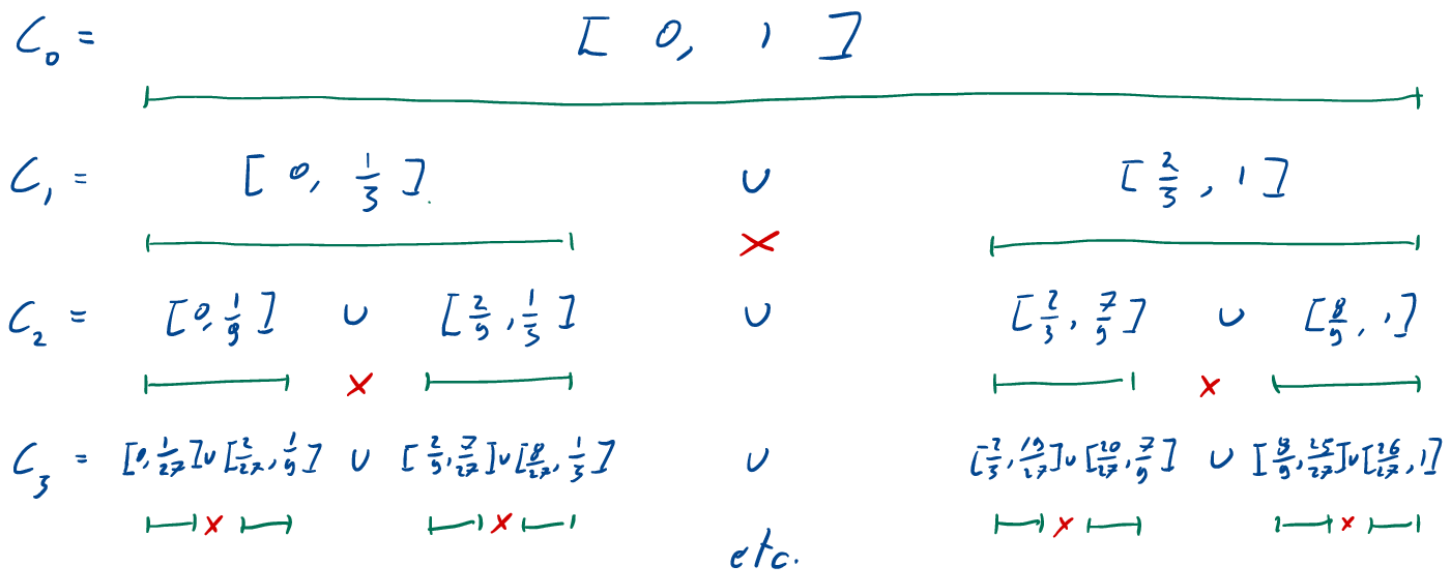
\includegraphics[width=12.5cm]{immagini/cantor.png}
\end{figure}

ovvero, preso l'intervallo $[0,1]$ possiamo dividerlo in tre parti e rimuovere la parte centrale $\left]\frac 13, \frac 23\right[$, chiamiamo gli intervalli rimanenti $C_1$, possiamo iterare il procedimento sui due segmenti di $C_1$ ed ottenere $C_2,C_3,\ldots, C_{n+1} = \frac{C_n}{3} \cup \left(\frac{C_n}{3} + \frac{2}{3}\right),\ldots$, a questo punto 
definiamo l'insieme di Cantor $C$ come:
\[ C := \bigcap_{i \in \NN}C_i
	\]
Esiste una funzione continua (e debolmente crescente) $f : \RR \to \RR$ detta \vocab{scala di Cantor} (o \vocab{scala del diavolo}), tale che $f^{\prime}(x) = 0$ per $x \not\in C$ e non è 
derivabile in $x \in C$.

\begin{figure}[H]
	\centering
	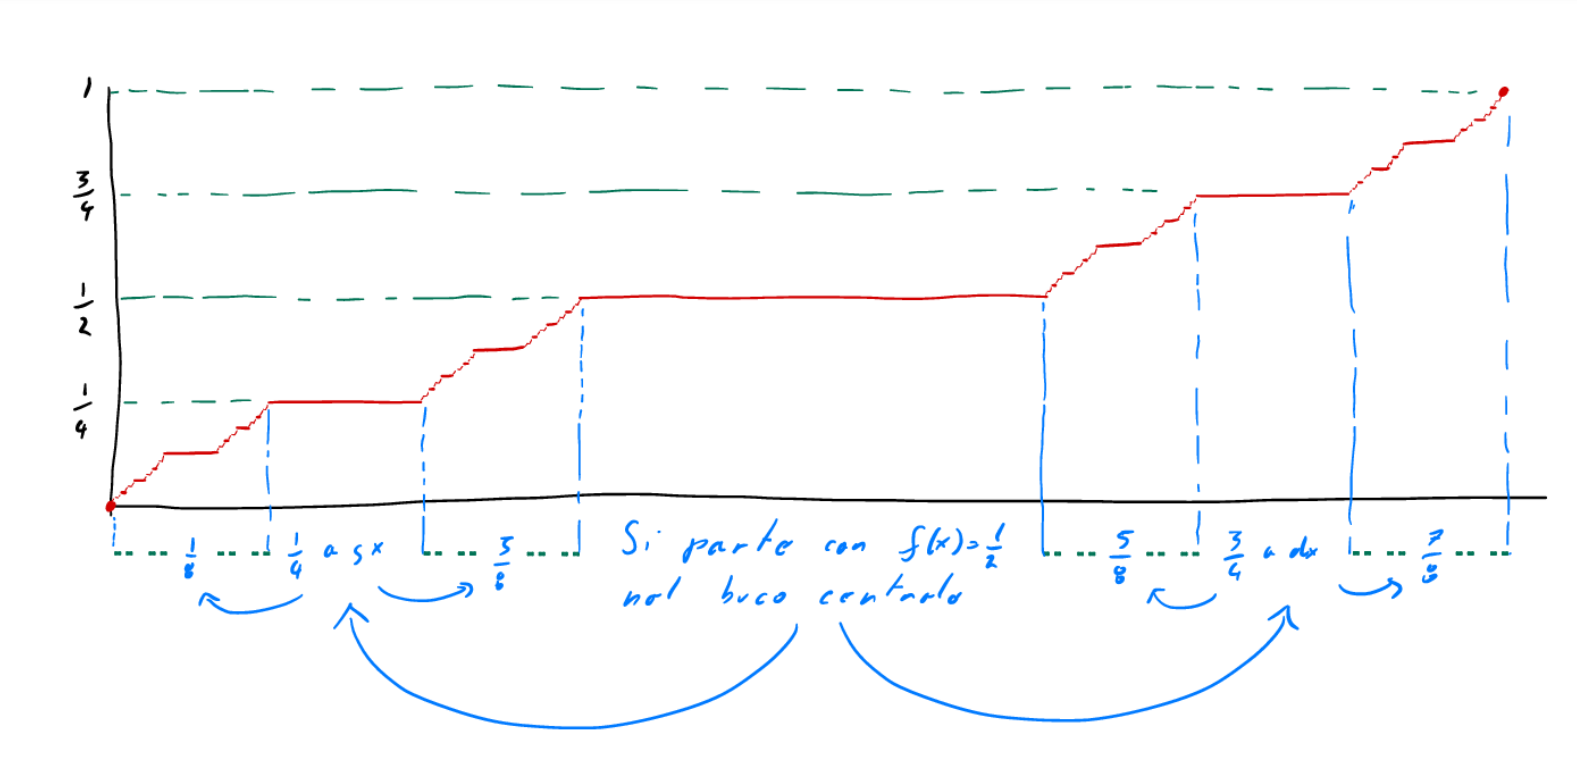
\includegraphics[width=13.5cm]{immagini/scalacantor.png}
\end{figure}

tale funzione si costruisce aggiungendo tratti costanti (prima $\frac 12$, poi $\frac 14$, $\frac 34$ e così via, dividendo l'intervallo $[0,1]$ sull'asse delle ordinate in parti uguali) alle parti eliminate sull'intervallo
$[0,1]$ sull'asse delle ascisse per costruire l'insieme di Cantor.

\begin{note}
Per $\QQ$ e $C$ non vale il \hyperref[unicità]{Fatto 1.5} ma, in realtà, sono di unicità.
\end{note}

\begin{exampleb}[$a_n \uparrow l$]
L'insieme degli elementi di una successione crescente col suo limite è un esempio di insieme di unicità.
\end{exampleb}

\begin{figure}[H]
	\centering
	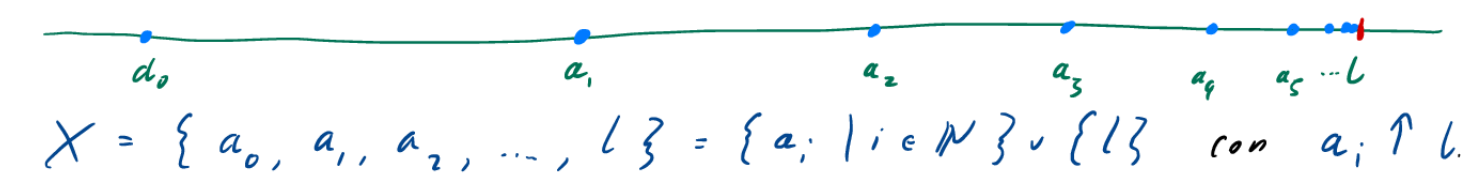
\includegraphics[scale=0.35]{immagini/succunic.png}
\end{figure}

Dimostriamo quindi che $X$ è un insieme di unicità.
\begin{proof}
Per ipotesi la funzione $f$ è lineare in $]-\infty, a_0[$ , $]a_0,a_1[$ , $]a_1,a_2[$ , $\ldots$ quindi nei punti $a_0,a_1,a_2,\ldots$ ammette ovviamente derivata destra e sinistra. 
Siccome, sempre per ipotesi, $f$ è continua e non ammette punti angolosi, questi punti non possono essere angolosi, per cui $f_{-}'(a_i) = f_{+}'(a_i)$, ovvero le rette $f_{|\,]-\infty, a_0[}$, $f_{|\,]a_0,a_1[}$, etc. hanno lo stesso coefficiente angolare.
Pertanto, per continuità, $f_{|\,]-\infty, l[}$ è lineare e per ipotesi lo è anche $f_{|\,]l,+\infty[}$, quindi $f$ è lineare.
\end{proof}

\begin{examplebb}[Successione di successioni crescenti]
L'insieme degli elementi di una successione crescente di successioni crescenti è un insieme di unicità.
\end{examplebb}

	\begin{figure}[H]
		\centering
		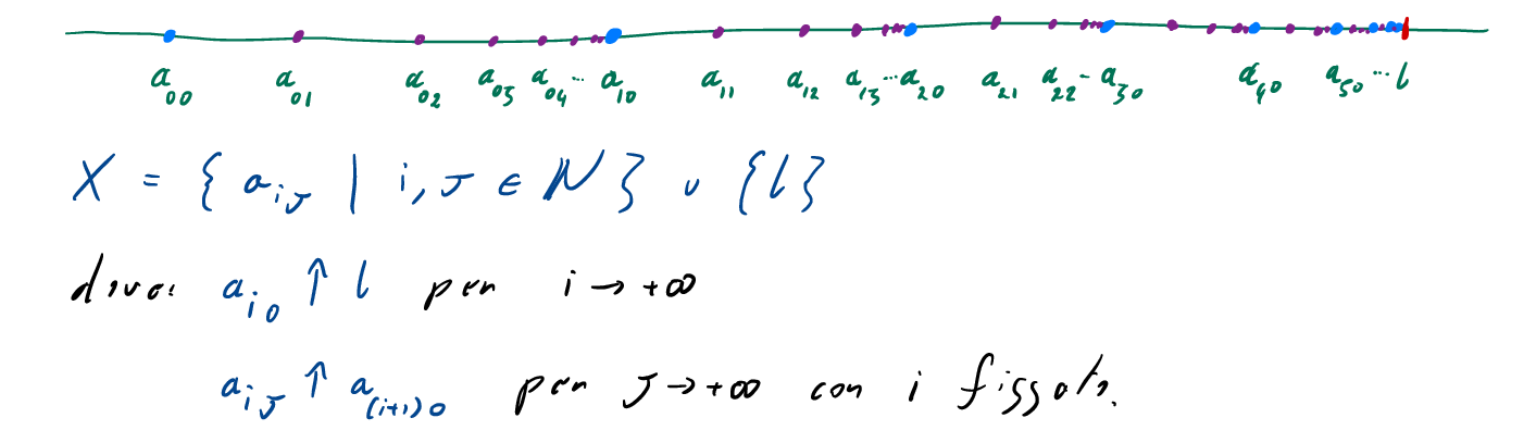
\includegraphics[width=12.5cm]{immagini/succunic2.png}
	\end{figure}

Dimostriamo che $X$ è di unicità.
\begin{proof}
In ciascuno degli intervalli $]a_{i0}, a_{(i+1)0}[$, $f$ è lineare, ragionando come nell'esempio precedente, ci siamo ridotti alla situazione
- di nuovo - dell'esempio precedente con $a_i^{\prime} = a_{i0}$.
\end{proof}

\subsection{Digressione: insiemi numerabili}
\begin{definition}
	Un insieme $X$ è \vocab{numerabile} se è il supporto di una successione, $X = \{a_0,a_1,a_2,\ldots\} = \{a_i | i \in \NN\}$, con $a_i \ne a_j$ per ogni $i \ne j$.\footnote{O in altre parole se esiste $f : \NN \to X$ biunivoca.}
\end{definition}

\begin{example}
	Alcuni esempi di insiemi numerabili sono:
	\begin{itemize}
		\item $\NN$, l'insieme dei numeri naturali, infatti, la successione $a_i = i$ realizza la bigezione.
		\item I numeri dispari, con la bigezione data da $a_i = 2i + 1$.
		\item I numeri primi, $a_i = p_i$, con $p_i$ $i$-esimo numero primo.
		\item $\ZZ$ l'insieme dei numeri interi, con la bigezione data da $a_i =  (-1)^i \left\lceil\frac{i}{2}\right\rceil$.
	\end{itemize}
\end{example}

\begin{examplem}
L'insieme $\NN \times \NN = \{(x,y) | x,y \in \NN\}$ è numerabile.
\end{examplem}

\begin{proof}
La funzione $f : \NN \times \NN \to \NN : (x,y) \longmapsto 2^x(1+2y) - 1$ è biunivoca (perché?), quindi $a_i = f^{-1}(i)$ enumera $\NN \times \NN$.
\end{proof}

\begin{proposition}
Un sottoinsieme infinito di un insieme numerabile è, a sua volta, numerabile.
\end{proposition}

\begin{proof}
Sia $Y \subseteq X$ con $Y$ infinito e $X = \{a_i | i \in \NN\}$. La sottosuccessione $b_j = a_{i_j}$ degli $a_*$ che appartengono a $Y$ enumera $Y$. A essere precisi 
bisognerebbe dire esattamente chi sono gli indici $i_j$. Per ricorsione:
\[ i_0 = \min\{i | a_i \in Y\} \qquad i_{j+1} = \min\{i > i_j | a_i \in Y\}
	\]
dove i minimi esistono perché $Y$ non è finito.
\end{proof}

\begin{proposition}
Se $X$ e $Y$ sono numerabili $X \times Y = \{(a,b) | a \in X, b \in Y\}$ è anch'esso numerabile.
\end{proposition}

\begin{proof}
Fissiamo $X = \{a_i | i \in \NN\}$, $Y = \{b_j | j \in \NN\}$. Siccome $\NN \times \NN$ è numerabile, $\NN \times \NN = \{(i_t,j_t)|t \in \NN\}$.
Quindi $X \times Y = \{(a_{i_t}, a_{j_t}) | t \in \NN\}$.
\end{proof}

\begin{example}
$\QQ$ è numerabile.
\end{example}

\begin{proof}
$\QQ$ è in corrispondenza biunivoca con:
\[F = \{(\text{num.},\text{den.})\footnote{num. = numeratore, den. = denominatore.} | \text{num. $\in \ZZ$} \wedge \text{den. $\in\NN_{>0}$} \wedge \text{M.C.D.(num.,den.) = 1}\} \subseteq \ZZ \times \NN\]
\end{proof}

\begin{notexample}
$\RR$ non è numerabile.
\end{notexample}

\begin{proof}
Supponendo, per assurdo, che $\RR = \{a_i | i \in \NN\}$, cerchiamo un $x \in \RR$ che non compare fra gli $a_i$. Allo scopo, costruiamo la sottosuccessione $a_{i_j}$
definita per ricorrenza da:
\[ i_0 = 0 \qquad i_1 = \min\{i | a_i > a_0\} \qquad i_{j+1} = \min\{i | \, \text{$a_i$ è compreso tra $a_{j-1}$ e $a_j$}\}
	\]
graficamente:

	\begin{figure}[H]
		\centering
		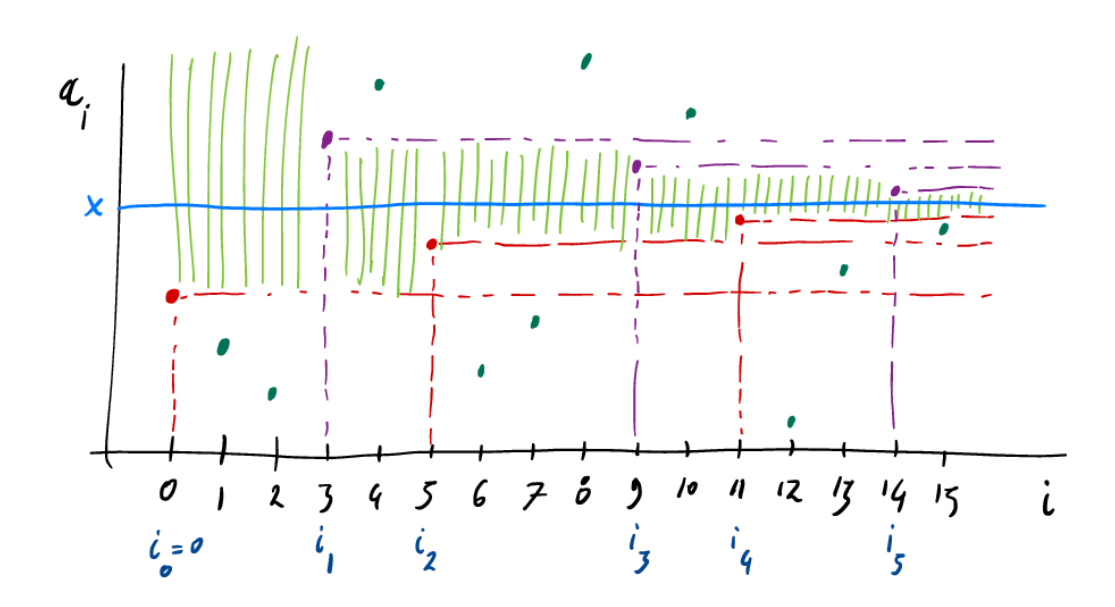
\includegraphics[width=10.5cm]{immagini/RRnum.png}
	\end{figure}

Si vede facilmente (esercizio!) che la successione $\{a_{i_{2k}}\}_k$ è crescente, $\{a_{i_{2k+1}}\}_k$ è decrescente 
e $ \lim_{k \to +\infty} a_{i_{2k}} \leq \lim_{k \to +\infty}a_{i_{2k+1}}$. Fissiamo $x$ tale che $ \lim_{k \to +\infty} a_{i_{2k}} \leq x \leq \lim_{k \to +\infty} a_{i_{2k+1}}$.
Chiaramente $x$ non è nessuno degli $a_{i_j}$, perché $a_{i_2k} < x < a_{i_{2k+1}}$. Supponiamo $x = a_n$, allora ci sarà $j$ tale che $i_j < n < i_{j+1}$, ma 
questo è assurdo perché allora $x = a_n$ è compreso fra $a_{i_{j-1}}$ e $a_{i_j}$, però $n < i_{j+1}$ contro la minimalità di quest'ultimo.

\begin{exercise}
Completare la dimostrazione nel caso $n < i$.
\end{exercise}

\begin{exercise}
Dimostrare che l'insieme di Cantor $C$ non è numerabile.
\end{exercise}
\end{proof}

\pagebreak
\subsection{Tornando agli insiemi di unicità}

\begin{theorem}
[Cantor-Lebesgue]
\label{CL}
Se $X \subseteq \RR$ è chiuso e numerabile, allora $X$ soddisfa $(\star)$, e quindi è di unicità.
\end{theorem}

La strategia di dimostrazione passa attraverso una definizione.

\begin{definition}
Dato $X \subseteq \RR$, il \vocab{derivato di Cantor-Bendixson} di $X$ è:
\[ X^{\prime} = X \setminus\{\text{punti isolati di $X$}\}
	\]
(dove $a \in X$ è un \vocab{punto di accumulazione} se $\exists \varepsilon > 0 :\, ]a - \varepsilon, a + \varepsilon[ \,\cap\, X = \{a\}$).
\end{definition}

\begin{remark}[Derivato di un chiuso soddisfa $(\star) \implies$ chiuso soddisfa $(\star)$]
Se $X$ è chiuso e $X^{\prime}$ soddisfa $(\star)$ - per cui $X'$ è di unicità per il criterio -, allora anche $X$ è di unicità.
\end{remark}

Dimostriamo questo fatto.

\begin{proof}
Occorre dimostrare che se $f : \RR \to \RR$ è continua, lineare quando ristretta agli intervalli aperti che non intersecano $X$, e non ha punti angolosi, allora $f$ è lineare, in tal modo sono soddisfatte le ipotesi del \hyperref[unicità]{Fatto 1.5} ed $X$ è di unicità.\\
Per fare ciò osserviamo che, data $f$ come sopra, se dimostriamo che quando è ristretta agli intervalli aperti che non intersecano $X'$ è lineare (e non avendo punti angolosi in generale quest'ipotesi è in automatico verificata) - essendo che quest'ultimo rispetta $(\star)$, cioè verifica le ipotesi del \hyperref[unicità]{Fatto 1.5} - allora si ottiene che $f$ è in generale lineare e quindi anche $X$ soddisfa le ipotesi del criterio.\\
Consideriamo un intervallo aperto che non interseca $X'$, $]a,b[ \,\cap\, X^{\prime} = \emptyset$, dobbiamo verificare che $f_{|\,]a,b[}$ è lineare. Ci basta dire che per ogni $\varepsilon > 0$, $f_{|[a+\varepsilon, b-\varepsilon]}$ è lineare - cioè che è lineare su ogni sottointervallo, dopodiché è banale che se vale per ogni $\varepsilon > 0$, vale in generale, e quindi $f_{|\,]a,b[}$ è lineare -.\\
Siccome per ipotesi $]a,b[ \, \cap \, X^{\prime} = \emptyset$, allora $]a,b[ \,\cap\, X \subseteq \{\text{punti isolati di $X$}\}$. Quindi l'intersezione con un sottointervallo chiuso $[a+\varepsilon, b-\varepsilon] \cap X$ è finita, se così non fosse, avrebbe che esiste nell'intersezione un punto di accumulazione 
$\alpha$ che naturalmente non può essere un punto isolato di $X\;\lightning$. Per cui $f_{|[a+\varepsilon, b-\varepsilon]}$ è lineare a tratti, e, siccome per ipotesi non ha punti angolosi (ed è continua), è lineare su tutto il sottointervallo.
\end{proof}

\begin{corollary}[Derivato $n$-esimo soddisfa $(\star) \implies$ insieme soddisfa $(\star)$]
Detto $X^{(n)}$ il derivato $n$-esimo di $X$, se per $X^{(n)}$ vale $(\star)$, per qualche $n \in \NN$, allora anche per $X$ vale $(\star)$, quindi per il \hyperref[unicità]{Fatto 1.5} è di unicità.\footnote{Il caso con $X^{(n)} = \emptyset$ scritto da Mamino nelle note è un caso particolare di questo.}
\end{corollary}

\begin{proof}
È una facile induzione su $n$, il caso $0$ è banale, mentre per il caso $n = 1$ vale l'osservazione vista sopra. Supponiamo ora che se $X^{(n-1)}$ soddisfa $(\star)$, allora 
anche $X$ soddisfa $(\star)$, e verifichiamo che se $X^{(n)}$ soddisfa $(\star)$ allora anche $X$ lo soddisfa.\\
Detto $X^{(n-1)} = Y$, allora $Y' = X^{(n)}$, dunque vale l'osservazione sopra, quindi $Y = X^{(n-1)}$ soddisfa $(\star)$ e per ipotesi induttiva anche $X$ soddisfa $(\star)$.
\end{proof}

Il guaio è che ci sono chiusi numerabili per cui $X^{(n)} \ne \emptyset$, qualunque sia $n$ - per cui non possiamo usare il corollario sopra per dedurre che sono di unicità -.

\begin{example}
Vogliamo costruire $X$ chiuso e numerabile tale che $X^{(n)} \ne \emptyset$ per ogni $n \in \NN$. Cominciamo col rivedere alcuni esempi già visti.
\end{example}

\begin{figure}[H]
		\centering
		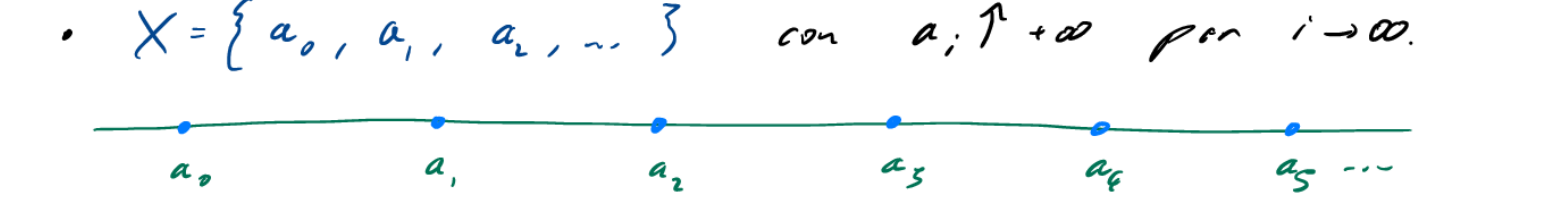
\includegraphics[scale = 0.3]{immagini/es1.png}
\end{figure}

Tutti i punti sono isolati, $X^{\prime} = \emptyset$.

\begin{figure}[H]
	\centering
	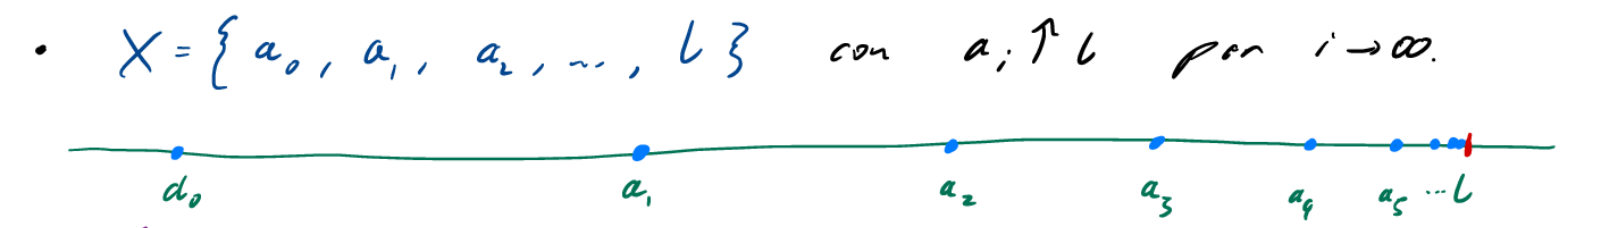
\includegraphics[scale = 0.3]{immagini/es2.png}
\end{figure}

``Successione con punto limite". Tutti i punti sono isolati salvo $l$, quindi $X^{\prime} = \{l\}$ e $X^{\prime\prime} = \emptyset$.

\begin{figure}[H]
	\centering
	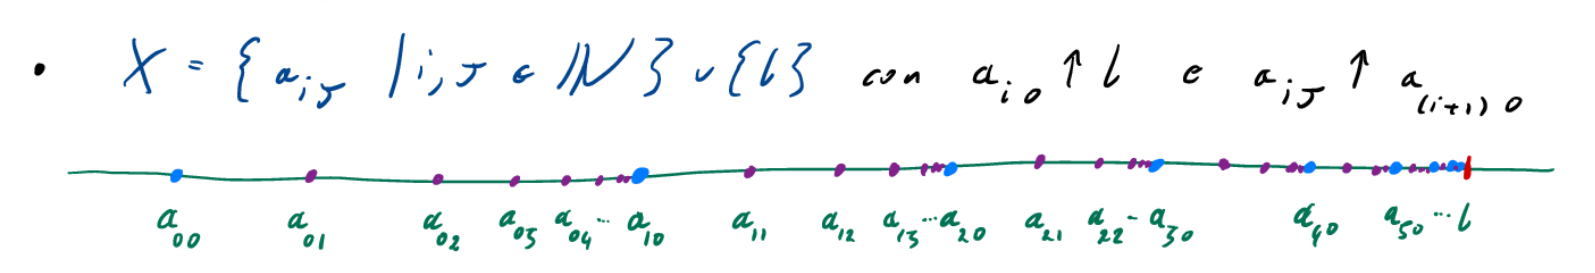
\includegraphics[scale = 0.3]{immagini/es3.png}
\end{figure}

``Successione di successioni", $X^{\prime} = \{a_{10}, a_{20}, \ldots, l\}$, $X^{\prime\prime} = \{l\}$ e $X^{\prime\prime\prime} = \emptyset$.\\
Si vede che possiamo proseguire, in qualche modo, costruendo una successione di successioni di successioni, etc. $n$ volte, $X_n$. Avremo $X_n^{(n)} \ne \emptyset$, $X_n^{(n+1)} = \emptyset$. Ora costruiamo 
$X_{\omega}$ fatto così:

\begin{figure}[H]
	\centering
	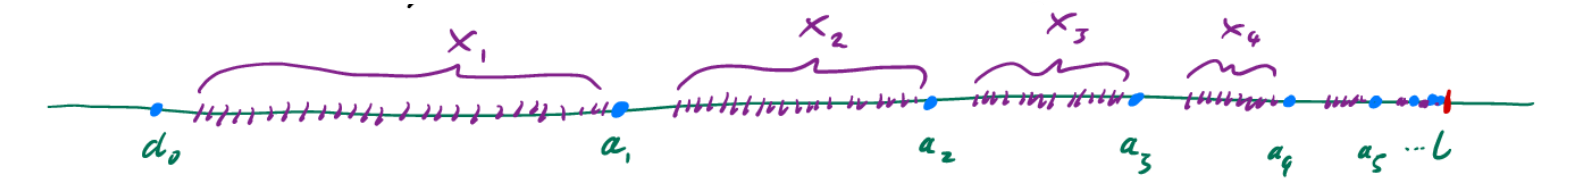
\includegraphics[scale = 0.3]{immagini/esomega.png}
\end{figure}

È chiaro che, per ogni $n$, $X_\omega^{(n)} \ne \emptyset$. D'altro canto, $X_\omega$ soddisfa il \hyperref[unicità]{Fatto 1.5}, perché $f$ deve essere lineare in ciascuno degli intervalli
$[a_n,a_{n+1}]$, perché $X_{n+1}$ soddisfa il \hyperref[unicità]{Fatto 1.5}, quindi ci si riduce al caso della successione.

\begin{exercise}
Perché $X_\omega$ è numerabile?
\end{exercise}

Ora potremmo pensare che, pazienza se $X_\omega$ non si smonta a furia di derivati, sarà un caso particolare. Però adesso, possiamo fare una successione di insiemi come $X_\omega$, chiamiamola $X_{\omega+1}$, e 
una successione di questi $X_{\omega+2}$, etc.\\
Al diavolo, serve un nuovo corollario!

\begin{corollary}
Se $X^{(n)}$ è di ``tipo $X_\omega$", allora per $X$ vale il \hyperref[unicità]{Fatto 1.5}.
\end{corollary}

Ok, questo corollario copre $X_\omega$, $X_{\omega + 1}$, $X_{\omega + 2}$, ma copre anche $X_{\omega \cdot 2}$?

\begin{figure}[H]
		\centering
		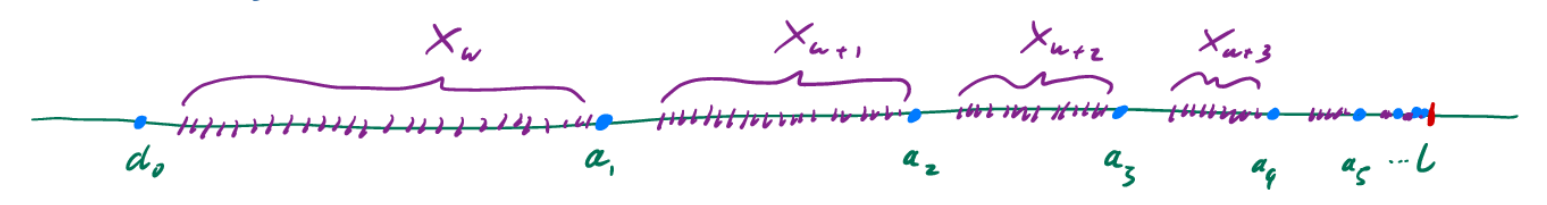
\includegraphics[scale = 0.3]{immagini/2omega.png}
\end{figure}

No: occorre un nuovo corollario.

\begin{corollary}
Se $X^{(n)}$ è di ``tipo $X_{\omega \cdot 2}$", allora per $X$ vale il \hyperref[unicità]{Fatto 1.5}.
\end{corollary}

E poi un altro per $X_{\omega \cdot 3}$, e un altro per $X_{\omega \cdot 4}$, etc.\\
E ora abbiamo finito? No, perché possiamo costruire una nuova successione con $X_{\omega},X_{\omega \cdot 2},X_{\omega \cdot 3}$, etc.\\
Se chiamiamo questa follia $X_{\omega \cdot \omega}$, ecco che si riparte a fare successioni di $X_{\omega \cdot \omega}$. Ora si sarà capito che definiremo
una serie aritmetica di queste cose, per cui potremo fare anche $\omega^\omega$, $\omega^{\omega^{\omega}}$, etc. È questa la soluzione allora?\\
No, ogni sforzo di trovare l'induzione a capo delle induzioni è vano. Se ho $X_{\omega}$, $X_{\omega^\omega}$, $X_{\omega^{\omega^{\omega}}}$, etc., allora,
ecco che faccio una successione con queste cose, la battezzo in qualche modo - ad esempio, $X_{\varepsilon_0}$ - e si riparte!\\
Per smontare ogni possibile insieme chiuso e numerabile occorre un \textbf{nuovo tipo di induzione}, l'\vocab{induzione transfinita}, che è strettamente più potente dell'induzione aritmetica.
Questa tecnica è stata sviluppata da Cantor, forse prendendo le mosse dal problema degli insiemi di unicità, e sarà uno degli argomenti centrali del corso.

\begin{exercise}[per la fine del corso]
Dimostrare il teorema di \hyperref[CL]{Cantor-Lebesgue}.
\end{exercise}

\subsection{Giochi di parole}
Descrivere un oggetto matematico non basta per crearlo. Se bastasse, si incorrerebbe in contraddizioni come queste.
\paragraph*{Paradosso di Russell}\mbox{}\\
Tipicamente le collezioni - uso questa parola perché daremo, al termine ``insieme", un senso tecnico preciso - non sono membro di se stesse: la collezione di 
tutti i numeri primi non è un numero primo. Però ci sono anche collezioni che sono membri di se stessi: per esempio la collezione di tutte le collezioni. Consideriamo:
\[ N = \{\text{collezioni $X$}\, | X \not\in X \}
	\]
la collezione delle collezioni che non sono membri di se stessi - la $N$ sta per collezioni normali. Quindi ci chiediamo se $N \in N$ oppure no? $N \in N$ se e solo se per definizione $N \not \in N$, che è assurdo.\\
Il paradosso di Russell ci dice che, del principio di collezione - ossia l'idea che data una proprietà ben definita $P$ si possa costruire la collezione $\{X | P(X)\}$ - non ci si può fidare.

\paragraph*{Paradosso di Berry}\mbox{}\\
L'italiano annovera un numero finito di parole, è quindi possibile formare solo un numero finito di frasi di meno di cento parole. Alcune di queste descrivono un numero naturale, altre no. Comunque, solo un numero 
finito di numeri naturali può essere descritto con meno di cento parole. Per il principio del minimo, esiste:
\begin{align*}
	h = \text{``il più piccolo numero naturale che l'italiano non può} \\ 
 \text{descrivere con meno di cento parole"}
\end{align*}
Il guaio chiaramente, è che lo abbiamo appena descritto con sedici parole.\\
Quindi non ci si può fidare troppo neppure dell'italiano, o meglio, non è possibile descrivere precisamente cosa sia una descrizione precisa.\\
In conclusione, occorre fissare un linguaggio formale in cui si esprimano le proposizioni della teoria degli insiemi, e occorre fissare un sistema di assiomi, espressi in questo linguaggio, che 
dicano quali costruzioni sono lecite: quali insiemi esistono. Il ruolo della teoria degli insiemi è, poi, di fondare l'edificio della matematica. L'ambizione, quindi, è che il linguaggio e gli assiomi della teoria degli insiemi, 
siano in realtà, il linguaggio e gli assiomi della matematica.

\subsection{Scopi del corso}
Questo corso persegue due obiettivi:
\begin{enumerate}[(1)]
	\item Studiare i \textbf{fondamenti della matematica}, nella forma più comunemente accettata nel XX secolo e fino ad ora, la teoria degli insiemi di 
	\href{https://it.wikipedia.org/wiki/Ernst_Zermelo}{\textcolor{purple}{Zermelo}}-\href{https://it.wikipedia.org/wiki/Adolf_Abraham_Halevi_Fraenkel}{\textcolor{purple}{Fraenkel}} con l'assioma della scelta (ZFC).
	\item Studiare tecniche e strumenti che sono stati sviluppati grazie alla teoria degli insiemi, per esempio: la teoria delle cardinalità, la teoria dei numeri ordinali, l'induzione e la ricorsione transfinita.
\end{enumerate}

In questo corso non ci occupiamo dei modelli della teoria degli insiemi. Mi spiego. Per esempio, in teoria dei gruppi si assiomatizza cosa sia un gruppo, e poi si studia come possano essere fatti i diversi gruppi. In 
teoria degli insiemi si assiomatizza l'universo di tutti gli insiemi, però, per il teorema di incompletezza di \href{https://it.wikipedia.org/wiki/Kurt_G%C3%B6del}{\textcolor{purple}{Gödel}}, questa assiomatizzazione non 
può essere completa. Quindi esistono tanti universi insiemistici possibili. Indagare queste possibilità - i modelli della teoria degli insiemi - è argomento di corsi più avanzati.

\section{Il linguaggio della teoria degli insiemi}
Per non incorrere in contraddizione, accettiamo che le sole proposizioni ad avere senso siano quelle esprimibili mediante \vocab{formule insiemistiche}. Le formule si costruiscono ricorsivamente.
\begin{itemize}
	\item Le lettere $a,b,c,\ldots,A,B,C,\ldots,\alpha,\beta,\gamma,\ldots$ rappresentano \vocab{variabili}. I valori delle variabili sono sempre insiemi, e non ci sono altri oggetti salvo gli insiemi.
	\item Le \vocab{formule atomiche} sono:
	\[ \text{variabile = variabile} \qquad \qquad \text{variabile $\in$ variabile}\footnote{\,``appartiene a".}
		\]
	sono formule atomiche $x=y$, $x=x$, $\alpha = C$, e anche $x \in y$, $x \in x$, $\alpha \in C$.
	\item Le formule atomiche si combinano tra loro mediante:
	\begin{itemize}
		\item \vocab{connettivi logici} ovvero il ``non'' la ``e'' e la ``o'' (inclusiva):
		\[ \text{$\neg$ formula} \qquad \text{formula $\land$ formula} \qquad \text{formula $\lor$ formula}
			\]
		quindi ad esempio:
		\begin{flalign*}
			&\neg\Phi \equiv \text{``$\Phi$ è falsa''} &\\
			&\Phi \land \psi \equiv \text{``$\Phi$ e $\psi$ sono entrambe vere''} &\\
			&\Phi \lor \psi \equiv \text{``almeno una fra $\Phi$ e $\psi$ è vera''}
		\end{flalign*}
		\item \vocab{quantificatori} ovvero quello universale ``per ogni'' e quello esistenziale ``esiste'':
		\[ \forall x \, \text{formula} \qquad \exists x \, \text{formula}
			\]
		ad esempio:
		\begin{flalign*}
			&\forall x \, \Phi \equiv \text{``$\Phi$ è vera qualunque sia l'insieme $x$''} &\\
			&\exists x \, \Phi \equiv \text{``c'è un insieme $x$ che fa si che $\Phi$ sia vera''}
		\end{flalign*}
		\begin{exercise}
			Chiaramente varranno $\forall x \, x = x,$ $ \forall x \, \exists y \, x = y,$ $ \neg (\exists x \, \forall y \, x = y)$.
		\end{exercise}
	\end{itemize}
\end{itemize}

\textbf{\underline{L'intuizione}} è che l'universo insiemistico sia un gigantesco \href{https://it.wikipedia.org/wiki/Digrafo_aciclico}{\textcolor{purple}{grafo diretto aciclico}} i cui vertici sono gli insiemi,
ed in cui le frecce rappresentano la relazione di appartenenza.

\begin{center}
	\begin{figure}[h]
		\centering
		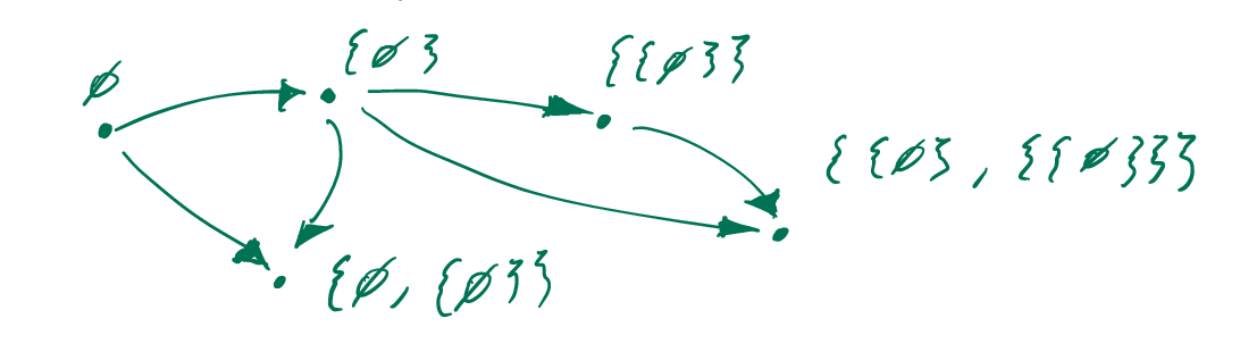
\includegraphics[width=10.5cm]{immagini/graf.png}
	\end{figure}
\end{center}

Possiamo solo fare affermazioni a proposito di vertici e frecce di questo grafo. Per esempio:
\[ \text{``$a$ è un elemento di un certo $b$''} \equiv \text{``c'è un percorso di due frecce fra $a$ e $b$''} 
	\]
che corrisponde mediante formule insiemistiche a $ \exists x (a \in x \land x \in b)$. E ancora:
\[\text{``$a$ è un sottoinsieme di $b$''} \equiv \text{``ogni elemento di $a$ è elemento di $b$''} \equiv \]\[
		\equiv\text{``non c'è un insieme che è elemento di $a$ e non di $b$''}\equiv\]\[
	 \equiv \text{``non c'è un vertice con una freccia verso $a$ e non una verso $b$''}
	\]
che corrisponde mediante formule insiemistiche a $\neg\exists x (x \in a \land \neg x \in b)$ (tutto ciò che raggiunge $a$ deve raggiungere anche $b$).\\
\textbf{\underline{Parentesi}} Ad essere precisi, avremmo dovuto definire le formule includendo un mucchio di parentesi, allo scopo di eliminare ogni possibilità
di formare una combinazione di simboli ambigua. Per esempio $\textcolor{red}{\Phi_1 \land \Phi_2 \lor \Phi_3}$ è ambigua, perché si potrebbe leggere $(\Phi_1 \land \Phi_2) \lor \Phi_3$
o $\Phi_1 \land (\Phi_2 \lor \Phi_3)$. In una notazione completamente parentesizzata, per esempio, la formula per ``$a$ è un sottoinsieme di $b$'' sarebbe:
\[ \neg(\exists x((x \in a)\land(\neg(x \in b))))
	\]
Non useremo, in generale, questa notazione, ma useremo le parentesi selettivamente per evitare ambiguità. \footnote{In questo caso si useranno più parentesi, qualora alcune formule risultassero più leggibili in tal modo.}\\
\textbf{\underline{Abbreviazioni}} Le formule appena descritte costituiscono il linguaggio della teoria degli insiemi \textbf{puro}. Durante il corso estenderemo
più volte questo linguaggio mediante abbreviazioni, che semplicemente rimpiazzano formule più lunghe con scritture convenzionali più compatte, e quindi non alterano 
la potenza espressiva del linguaggio. Vediamo le prime abbreviazioni:
\[ x \ne y \Mydef \neg x = y \footnote{Cioè ``non è vero che $x$ è uguale a $y$''.} \qquad x \not\in y \Mydef \neg x \in y \qquad \not\exists x \,\Phi \Mydef \neg \exists x \, \Phi
	\]\[ \Phi \rightarrow \psi \Mydef \psi \lor \neg \Phi \qquad \Phi \leftrightarrow \psi \Mydef (\Phi \rightarrow \psi) \land (\psi \rightarrow \Phi)
		\]\[ \exists x \in y \; \Phi \Mydef \exists x (x \in y \land \Phi) \qquad \forall x \in A \; \Phi \Mydef \forall x (x \in A \rightarrow \Phi)
			\]\[ \exists !\, x\, \Phi(x) \Mydef \exists x (\Phi(x) \land \forall y(\Phi(y) \rightarrow y = x))
				\]\[ \exists !\, x \in A \,\Phi(x) \Mydef \exists! \, x(x \in A \land \Phi(x))
					\]\[ A \subseteq B \Mydef \forall x (x \in A \rightarrow x \in B) \qquad A \subsetneq B \Mydef( A \subseteq B) \land (A \ne B)
						\]\[ C = A \cup B \Mydef \forall x \, x \in C \leftrightarrow (x \in A \lor x \in B)
							\]\[ C = A \cap B \Mydef \forall x \, x \in C \leftrightarrow (x \in A \land x \in B)
								\]
\begin{note}
	Il fatto che possiamo dire $C = A \cup B$ o $C = A \cap B$ non significa né che questi oggetti esistano né che siano unici. Dimostreremo fra poco l'esistenza e unicità 
	di unione e intersezione.
\end{note}

\begin{exercise}
Esprimi queste proposizioni mediante formule insiemistiche pure:
\begin{itemize}
	\item gli elementi degli elementi di $A$ sono elementi di $A$;
	\item $B$ è l'insieme dei sottoinsiemi di $A$;
	\item l'unione degli elementi di $A$ è l'intersezione di quelli di $B$\footnote{Qui assumi che l'unione e intersezione esistano e siano uniche.}
\end{itemize}
\end{exercise}

\subsection{Le regole di inferenza}
La teoria assiomatica degli insiemi si compone di tre parti: il linguaggio formale che abbiamo appena descritto, gli assiomi della teoria che studieremo durante il corso, 
ed un sistema di regole che specificano precisamente quali passaggi sono leciti nelle dimostrazioni. Possiamo immaginare questa ultima componente come una specie di algebra dei ragionamenti,
che permette di verificare i passaggi di una dimostrazione in maniera puramente meccanica, come se fossero semplici manipolazioni algebrica. Noi non vedremo le regole di inferenza, e voglio spiegare qui il perché.
\begin{enumerate}[1]
	\item Sono argomento del corso di logica.
	\item In realtà, scrivere le dimostrazioni in maniera formale, le renderebbe lunghissime e particolarmente incomprensibili.
	\item In pratica, non si sbaglia facendo ragionamenti che non reggono, si sbaglia dicendo cose fumose che non possono essere espresse nel linguaggio della teoria. Per esempio, le parole ``e così via'' sono pericolose.
	\item Conoscere le regole - fidatevi - non aiuta né a trovare né a capire le dimostrazioni.
\end{enumerate}
Pur senza dare un sistema completo di regole, vediamo qualche manipolazione formale che potrebbe servire.\\
\textbf{\underline{Tavole di verità}} Due combinazioni mediante connettivi logici ($\neg$, $\land$, $\lor$, $\rightarrow$, $\leftrightarrow$)
delle stesse formule - ``\vocab{combinazioni booleane}'' - alle volte, dicono la stessa cosa. Per esempio, $\neg \Phi \lor \neg \psi \equiv\footnote{\,``equivale a''.} \neg (\Phi \land \psi)$.
Per verificare questo fatto basta considerare tutte le possibili combinazioni di valori di verità che possono assumere le formule combinate - nell'esempio $\Phi$ e $\psi$ - compilando una ``\vocab{tabella di verità}''.
\begin{center}
	\begin{tabular}{>{$}l<{$}>{$}l<{$}|*{7}{>{$}l<{$}}}
	\Phi & \psi & \neg\Phi   & \neg\psi   & \neg\Phi \lor \neg\psi   & \Phi \land \psi & \neg(\Phi \land \psi)    \\
	\hline\vrule height 14pt width 0pt
	V & V & F & F & \textcolor{red}{F} & V & \textcolor{red}{F}\\
	V & F & F & V & \textcolor{red}{V} & F & \textcolor{red}{V}\\
	F & V & V & F & \textcolor{red}{V} & F & \textcolor{red}{V}\\
	F & F & V & V & \textcolor{red}{V} & F & \textcolor{red}{V}
	\end{tabular} 
\end{center}
Come si osserva le due colonne corrispondenti ai valori di verità delle nostre formule iniziali hanno gli stessi valori di verità in ogni caso.\\
Conviene tenere a mente alcune delle equivalenze elementari:
\[ \neg\neg \Phi \equiv \Phi \qquad \Phi \land (\psi \lor \Theta) \equiv (\Phi \land \psi) \lor (\Phi \land \Theta) \qquad \Phi \lor (\psi \land \Theta) \equiv (\Phi \lor \psi) \land (\Phi \lor \Theta)
	\]\[ \neg(\Phi \land \psi) \equiv \neg \Phi \lor \neg \psi \qquad \neg(\Phi \lor \psi) = \neg \Phi \land \neg \psi \, \footnote{\href{https://it.wikipedia.org/wiki/Leggi_di_De_Morgan}{\textcolor{purple}{Leggi di De Morgan}}.}
		\]\[ \Phi \rightarrow \neg \psi \equiv \psi \rightarrow \neg \Phi \qquad \Phi \rightarrow \psi \equiv \neg \psi \rightarrow \neg \Phi
			\]

\begin{exercise}
Dimostrare le equivalenze delle formule elencate sopra.
\end{exercise}

Per quanto riguarda i quantificatori ricordiamo le regole seguenti, che tuttavia non sono esaustive.
\[ \neg\forall x \, \Phi \equiv \exists x \, \neg\Phi \qquad \neg\forall x \, \neg \Phi \equiv \exists x \, \Phi
	\]\[ \neg\exists x \, \Phi \equiv \forall x \, \neg \Phi \qquad \neg \exists x \, \neg \Phi \equiv \forall x \, \Phi
		\]

\begin{exercise}
Convinciti della validità delle equivalenze precedenti.
\end{exercise}

\begin{exercise}
Dimostra che:
\[ \neg \forall x \in A \, \Phi \equiv \exists x \in A \, \neg \Phi \qquad \neg \exists x \in A \, \Phi \equiv \forall x \in A \, \Phi
	\]
\end{exercise}

\begin{exercise}
Dimostra che:
\[ \forall x (x \in A \rightarrow x \in B) \equiv \neg \exists x (x \in A \land \neg x \in B)
	\]
\end{exercise}

\begin{exercise}
Secondo te, la seguente formula è vera?
\[ \forall A ((\exists x \, x \in A) \rightarrow \exists x \in A (x \in B \rightarrow \forall y \in A \, y \in B))
	\]
\end{exercise}

Infine vi sono regole per la relazione di uguaglianza, che dicono, in sostanza, che se $x = y$ allora $x$ e $y$ non sono distinguibili, ossia vale $\Phi(x) \leftrightarrow \Phi(y)$ qualunque sia $\Phi$.
Per quanto ci riguarda, \textbf{se $x = y$ allora $x$ e $y$ sono nomi della stessa cosa}.
\section{I primi assiomi}
\subsection{Assiomi dell'insieme vuoto e di estensionalità}
\begin{axiom}
[Assioma dell'insieme vuoto]
\label{ax1}
Esiste un insieme vuoto.
\[ \exists x \; \forall y \; y \not\in x
		\]
\end{axiom}

\begin{note}
Questo assioma non sarebbe strettamente necessario, in quanto potremmo ottenere un insieme vuoto anche come sottoprodotto, per esempio, dell'assioma dell'infinito che vedremo in seguito.
Tuttavia è bello poter partire avendo per le mani almeno un insieme.
\end{note}

\begin{axiom}
[Assioma di estensionalità]
\label{ax2}
Un insieme è determinato dalla collezione dei suoi elementi. Due insiemi coincidono se e solo se hanno i medesimi elementi.
\[ \forall a \; \forall b \; a = b \leftrightarrow \forall x (x \in a \leftrightarrow x \in b)
	\]
\end{axiom}

\begin{exercise}
Dimostra che la freccia $a = b \rightarrow \forall x (x \in a \leftrightarrow x \in b)$, in realtà, segue dal fatto che se $a = b$ allora $a$ e $b$ sono indistinguibili\footnote{Nel senso che abbiamo descritto in precedenza, cioè sono nomi della stessa cosa.}.
\end{exercise}

\textbf{\underline{Convenzione}} Le variabili libere (= non quantificate), se non specificato altrimenti, si intendono quantificate universalmente all'inizio della formula. Per cui possiamo scrivere
l'assioma di estensionalità semplicemente nella forma:
\[ a = b \leftrightarrow \forall x (x \in a \leftrightarrow x \in b)
	\]

\begin{proposition}[Unicità dell'insieme vuoto]
C'è un unico insieme vuoto.
\[ \exists ! \, x \; \forall y \; y \not \in x
	\]
\end{proposition}

\begin{proof}
Consideriamo due insiemi vuoti $x_1$ e $x_2$, ossia supponiamo $\forall y \, y \not\in x_1$, e $\forall y \, y \not \in x_2$. Allora:
\[ \forall y (y \in x_1 \leftrightarrow y \in x_2)
	\]
[sono coimplicate logicamente] perché $y \in x_1$ e $y \in x_2$ sono entrambe necessariamente false (quindi la proposizione così com'è scritta è sempre vera). Per \hyperref[ax2]{estensionalità}, la proposizione sopra (sempre vera) è equivalente a $x_1 = x_2$ (che quindi a sua volta sarà sempre vera), e quindi abbiamo la tesi.
\end{proof}

\emph{Dimostrazione formale.} Questo livello di pedanteria non è necessario, ma, per una volta, proviamo a dimostrare in ogni dettaglio la formula $\exists ! x (\forall y (y \not \in x))$. Per definizione di $\exists !$, ciò equivale a:
\[ \exists x_1 ((\forall y \, y \not \in x_1) \land \forall x_2 ((\forall y \, y \not \in x_2) \rightarrow x_2 = x_1))
	\]
Per l'\hyperref[ax1]{assioma del vuoto}, $\exists x_1 \, \forall y \, y \not \in x_1$: fissiamo questo $x_1$. Resta da dimostrare che:
\[ (\forall y \, y \not \in x_1) \land \forall x_2(\forall y \, y \not \in x_2) \rightarrow x_2 = x_1
	\]
Per costruzione, $\forall y \, y \not\in x_1$, è vera (avendo fissato $x_1$), quindi resta:
\[ \forall x_2 (\forall y \, y \not \in x_2) \rightarrow x_2 = x_1
	\]
Ora prendiamo un $x_2$ qualunque, dobbiamo dimostrare:
\[ \forall y (y \not \in x_2) \rightarrow x_2 = x_1
	\]
Si danno due casi: o $\forall y (y \not \in x_2)$ è vera o è falsa. Nel secondo caso, l'implicazione è vera per via della tabella di verità. Nel primo abbiamo sia $\forall y \, y \not \in x_1$, [vera] per
costruzione, sia $\forall y \, y \not \in x_2$, [vera] per ipotesi. Quindi, preso un qualunque $y$, $y \in x_1$ e $y \in x_2$ sono entrambe false. La tabella di verità di $\leftrightarrow$ ci dice quindi che vale $y \in x_1 \leftrightarrow y \in x_2$, e, per 
l'arbitrarietà di $y$:
\[ \forall y (y \in x_1 \leftrightarrow y \in x_2)
	\]
Dall'\hyperref[ax2]{assioma di estensionalità}:
\[ \forall y (y \in x_1 \leftrightarrow y \in x_2) \rightarrow x_1 = x_2
	\]
Abbiamo quindi $x_1 = x_2$, da cui segue la verità dell'implicazione iniziale. $\hfill\square$


Chiaramente, ho voluto scrivere questa dimostrazione delirante per convincervi che NON È UNA BUONA IDEA.

\begin{notation}
L'unicità dell'insieme vuoto ci giustifica ad introdurre delle nuove abbreviazioni:
\[ x = \emptyset \Mydef \forall y \, y \not\in x \qquad \emptyset \in x \Mydef \exists z (z = \emptyset \land z \in x)
	\]
\end{notation}

\subsection{Assioma di separazione}
\begin{axiom}
[Assioma di separazione]
\label{ax3}
Se $A$ è un insieme, e $\psi(x)$ una formula insiemistica qualunque, allora $\{x \in A | \psi (x)\}$\footnote{Stiamo usando già questa notazione, ma la definiremo a breve.} è un insieme.
\[ \forall A \; \exists B \; \forall x \; x \in B \leftrightarrow (x \in A \land \psi (x))
	\]
\end{axiom}

\begin{note}
Tecnicamente l'assioma di separazione è uno \vocab{schema di assiomi}, ossia una regola che, per ogni possibile formula $\psi$, ci permette di scrivere un assioma.
\end{note}

\begin{proposition}
Fissati $A$ e $\psi(x)$, l'insieme $\{x \in A | \psi(x)\}$ è univocamente definito. Ossia:
\[ \forall A \; \exists \textcolor{red}{!} B \; \forall x \; x \in B \leftrightarrow (x \in A \land \psi(x))
	\]
\end{proposition}

\begin{proof}
Come per l'unicità dell'insieme vuoto, supponiamo di avere $B_1$ e $B_2$ tali che:
\[ \forall x \, x \in B_1 \leftrightarrow (x \in A \land \psi(x)) \qquad \forall x \, x \in B_2 \leftrightarrow (x \in A \land \psi(x))
	\]
Allora, $\forall x \, x \in B_1 \leftrightarrow (x \in A \land \psi(x)) \leftrightarrow x \in B_2$, quindi ciò coimplica, per \hyperref[ax2]{estensionalità}, che $B_1 = B_2$.
\end{proof}

\begin{exercise}[Transitività della coimplicazione]
Verificare che se $\psi \leftrightarrow \Phi$ e $\Phi \leftrightarrow \Theta$, allora $\psi \leftrightarrow \Theta$.
\end{exercise}

\begin{notation}
Vista l'unicità, possiamo introdurre una nuova abbreviazione:
\[ B = \{x \in A | \psi(x)\} \Mydef \forall x \, x \in B \leftrightarrow (x \in A \land \psi(x))
	\]
\end{notation}

Osserviamo che l'assioma di separazione è una forma indebolita del principio di collezione\footnote{Quel principio che definisce gli insiemi come tutte le cose che soddisfano una certa formula.}. Rimpiazzando il principio con questo assioma, il Paradosso di Russell diventa una proposizione.

\begin{proposition}[Insieme di tutti gli inisemi]
Non esiste l'insieme di tutti gli insiemi.
\[ \not\exists V \; \forall x \; x \in V
	\]
\end{proposition}

\begin{proof}
Supponiamo, per assurdo, che esista questo $V$. Allora, per \hyperref[ax3]{separazione} con la formula $\psi (x) \equiv x \not \in x$, esiste l'insieme:
\[ N = \{x \in V | x \not\in x\}
	\]
che, per definizione (via separazione), ha la proprietà:
\[ \forall x \, x \in N \leftrightarrow (x \in V \land x \not \in x)
	\]
Per ipotesi assurda, $x \in V$ è sempre vera (stiamo considerando l'insieme di tutti gli insiemi), quindi quanto scritto si riduce a:
\[ \forall x \, x \in N \leftrightarrow x \not\in x
	\]
prendendo ora come insieme $N$: $x = N$, abbiamo $N \in N \leftrightarrow N \not\in N$, assurdo.
\end{proof}

\subsection{Classi e classi proprie}
Sebbene, abbiamo detto che gli unici oggetti della teoria degli insiemi sono gli insiemi, usualmente ci si riferisce alla collezione di tutti gli insiemi 
che soddisfano una certa formula come ad una specie di insieme: una \vocab{classe}. Più precisamente, data una formula $\psi(x)$, se diciamo: ``sia $C$ la classe degli insiemi $x$ tali che $\psi(x)$''
intendiamo dire che useremo la scrittura $x \in C$ come una semplice abbreviazione per la formula $\psi(x)$.\footnote{Ovvero per tutti gli oggetti (solo gli insiemi in questo caso) che soddisfano una tale formula $\psi(x)$.} \\
Non avrebbe senso scrivere \textcolor{red}{$C \in$ qualcosa}, perché il simbolo $\in$ in $x \in C$ non ha senso (ha senso solo tra oggetti di tipo insieme), se non nel tutt'uno $\in C$. In altri termini, se scriviamo $x \in C$ in luogo di $\psi(x)$ è solo come ausilio dell'intuizione (per comodità insomma, senza intendere qualcosa di formale all'interno della teoria degli insiemi):
avremmo potuto decidere di scrivere $x$\ding{168}, o nient'altro che $\psi(x)$.

\begin{definition}[Classe universale]
La classe $V$ si dice \vocab{classe universale} ed è la classe di tutti gli insiemi.
\[ x \in V \Mydef x = x \footnote{Cioè la classe degli insiemi che soddisfano il predicato $\psi(x): x = x$ (ovvero tutti gli insiemi per quanto assunto all'inizio della teoria), $V = \{x | \psi(x)\} = \{x | x = x\}$ (dove naturalmente non sto usando separazione ma il principio di collezione perché stiamo definendo una classe).}
	\]
\end{definition}

Insomma, scrivere $x \in V$ non dice molto: è una formula sempre vera.

\begin{notation}[Uguaglianza tra classi]
Date due classi $C$ e $D$, che, ricordiamo, non significa altro che ``date due formule$\ldots$'', definiamo l'abbreviazione:
\[ C = D \Mydef \forall x ((x \in C) \leftrightarrow (x \in D)) \footnote{Non è altro che un abbreviazione per dire che le formule che definiscono le classi $C$ e $D$ sono soddisfatte dagli stessi insiemi $x$.}
	\]
\end{notation}

Ora, dato un qualunque insieme $A$, possiamo definire la classe $\hat{A}$ degli $x$ tali che $x \in A$ (cioè la classe degli $x$ che soddisfano $\psi(x) : x \in A$). Se $\hat{A} = \hat{B}$, per l'abbreviazione data non stiamo dicendo altro che:
\[ \forall x ((x \in A) \leftrightarrow (x \in B))
	\]
che equivale $A = B$ per \hyperref[ax2]{estensionalità}. Ha quindi senso, con un leggero abuso di notazione, omettere il cappelletto $\hat{}$ e ``identificare'' la classe $\hat{A}$ semplicemente con $A$. In questo senso,
abbiamo classi che sono insiemi - formalmente $C$ è un insieme se $C = \hat{A}$ per qualche insieme $A$ - e classi che non sono insiemi. Chiamiamo \vocab{classe propria} una classe che non è un insieme.\footnote{Essere un insieme per una classe significa quindi moralmente identificarvisi nel senso riportato sopra, se ciò non fosse possibile parliamo di classi proprie.}

\begin{example}
$V$ è una classe propria.
\end{example}

\textbf{\underline{L'intuizione}}, che sarà più chiara via via che procediamo nel corso, è che le classi proprie sono troppo grandi per essere insiemi.

\subsection{Assioma del paio e coppia di Kuratowski}
I primi tre assiomi ci dicono, a grandi linee, che, entro i limiti di quanto si può fare rinunciando al principio di collezione - che esiste $\{x | \, \text{una qualunque proprietà}\}$ -, gli insiemi sono delle specie di collezioni.
Sono determinati dai loro elementi, e li si può dividere in collezioni più piccole in maniera arbitraria. \\ Ci troviamo, però, adesso, nella necessità di procurarci qualche insieme con cui lavorare. I prossimi assiomi serviranno per giustificare le costruzioni con cui,
usualmente, si definiscono nuovi insiemi. Per esempio, abbiamo bisogno di costruire certi insiemi di base, tipo l'insieme dei numeri interi o insiemi finiti i cui elementi sono elencati esplicitamente, fare prodotti di insiemi esistenti, 
considerare le funzioni fra insiemi esistenti, etc.

\begin{axiom}
[Assioma del paio]
\label{ax4}
Dati $a$ e $b$ esiste l'insieme $\{a,b\}$.
\[ \forall a \; \forall b \; \exists P \; \forall x \; x \in P \leftrightarrow (x = a \lor x = b)
	\]
\end{axiom}

\begin{proposition}
[Unicità del paio]
Fissati $a$ e $b$, l'insieme $\{a,b\}$ è univocamente determinato.
\[\forall a \; \forall b \; \exists\textcolor{red}{!} P \; \forall x \; x \in P \leftrightarrow (x = a \lor x = b)
	\]
\end{proposition}

\begin{exercise}
	Dimostra la proposizione precedente.
\end{exercise}

\begin{soln}
	Supponiamo che esistano $P_1$ e $P_2$ tali che:
	\[ \forall x (x \in P_1 \leftrightarrow (x = a \lor x = b)) \qquad \text e \qquad \forall x (x \in P_2 \leftrightarrow (x = a \lor x = b))
		\]
	da ciò segue che:
	\[ \forall x (x \in P_1 \leftrightarrow x \in P_2)
		\]
	dunque per \hyperref[ax2]{estensionalità} l'espressione sopra equivale a $P_1 = P_2$.
\end{soln}

\begin{proposition}[Esistenza dei singoletti]
	Dato $a$, esiste ed è unico $\{a\}$.
	\[ \forall a \; \exists ! S \; \forall x \; x \in S \leftrightarrow x = a
		\]
\end{proposition}

\begin{proof}
	Ponendo $b = a$ nella proposizione precedente, si ha che:
	\[ \forall a \; \exists ! S \; \forall x \; x \in S \leftrightarrow (x = a \lor x= a)
		\]
	ora $x = a \lor x = a$ equivale a $x = a$\footnote{Stiamo dicendo che in generale $\{a,a\} = \{a\}$ poiché $a \lor a = a$ (in base alle regole dei connettivi logici).}.
\end{proof}

\begin{notation}[Paio (o coppia) e singoletto]
	Possiamo ora introdurre delle abbreviazioni per il paio (o coppia) ed i singoletti:
	\[ P = \{a,b\} \Mydef \forall x \, x \in P \leftrightarrow (x = a \lor x = b)
		\]\[ S = \{a\} \Mydef \forall x \, x \in S \leftrightarrow x = a
			\]
\end{notation}

\begin{remark}
	Osserviamo che $\{a,b\} = \{b,a\}$.
\end{remark}

\begin{proof}
	Segue dal fatto che $\lor$ è commutativo:
	\[ x \in \{a,b\} \leftrightarrow (x = a \lor x = b) \leftrightarrow (x = b \lor x = a) \leftrightarrow x \in \{b,a\}
		\]
	quindi per \hyperref[ax2]{estensionalità} $\{a,b\} = \{b,a\}$.
\end{proof}

Il paio $\{a,b\}$ è, quindi, una coppia non ordinata. È possibile codificare le coppie ordinate con il seguente trucco.

\begin{definition}
	[Coppia di \href{https://it.wikipedia.org/wiki/Kazimierz_Kuratowski}{\textcolor{purple}{Kuratowski}}]
	Definiamo la \vocab{coppia di Kuratowski}:
	\[(a,b) \Mydef \{{a},\{a,b\}\}
		\]
\end{definition}

\begin{proposition}[Proprietà di coppia ordinata]
	La coppia di Kuratowski $(a,b)$ rappresenta la coppia ordinata di $a$ e $b$, ossia vale che:
	\[ (a,b) = (a^{\prime},b^{\prime}) \leftrightarrow (a = a^{\prime} \land b = b^{\prime})
		\]
\end{proposition}

\begin{proof}
	Detto $c = (a,b)$, vogliamo determinare univocamente $a$ e $b$. Osserviamo che $a$ è determinata da:
	\[ x = a \leftrightarrow \forall y \in c (x \in y) \, \footnote{Sostanzialmente stiamo dicendo che $a$ è identificato univocamente come l'elemento che appartiene ad entrambi gli elementi di $(a,b)$.}
		\]
	la freccia $\rightarrow$ segue da come è definita la coppia $(a,b)$, mentre $\leftarrow$ segue dal fatto che, sempre per definizione di coppia di Kuratowski, $\{a\} \in c = (a,b)$, per cui:
	\[ \forall y \in c (x \in y) \overset{\text{ipotesi}}{\implies} x \in \{a\} \overset{\text{singoletto}}{\implies} x = a
		\]
	Determiniamo ora univocamente $b$. Studiamo prima il caso in cui $\exists ! x (x \in c)$ - cioè il caso in cui abbiamo $(x,x) = \{\{x\}\}$ -:
	\[	\exists ! x (x \in c) \iff \{a\} = \{a,b\} \iff b = a
		\]
	In questo caso $b$ è determinato. Se non fosse così allora $\{a,b\}$ avrebbe due elementi distinti e $b$ sarebbe univocamente determinato da:
	\[ x = b \leftrightarrow (x \in \{a,b\} \land x \ne a)
		\]
\end{proof}

\begin{definition}[$n$-upla ordinata]
	Possiamo estendere la definizione di coppia ordinata con il seguente trucco:
	\begin{align*}
	   (a,b,c) &\Mydef ((a,b),c) \\
	   (a,b,c,d) &\Mydef (((a,b),c),d) \\
	   (a_1,a_2,\ldots,a_n) &\Mydef ((a_1,a_2,\ldots,a_{n-1}),a_n)
	\end{align*}
\end{definition}

\begin{note}
	Quest'ultima definizione è, in realtà, uno schema di definizioni: una per ogni $n$. Per ora, \textcolor{red}{NON} siamo in grado di scrivere, per esempio,
	una formula insiemistica che dica ``Esiste un $n$ ed una $n$-upla $(a_1,\ldots,a_n)$ tale che…''. Però, per ogni $n$ dato, chessò 92, possiamo scrivere esplicitamente una formula che dice $x = (a_1,a_2,a_3,\ldots,a_{92})$.
\end{note}

\begin{proposition}[Proprietà di $n$-upla ordinata]
	Si ha che:
	\[ (a,b,c) = (a',b',c') \leftrightarrow a = a' \land b = b' \land c = c'
		\]\[ (a_1,\ldots,a_n) = (a_1',\ldots,a_n') \leftrightarrow a_1 = a_1' \land \ldots \land a_n = a_n'
			\]
\end{proposition}

\begin{exercise}
	Dimostra la prima e convinciti che, dato un qualunque $n$ esplicito, potresti dimostrare la seconda.
\end{exercise}

\subsection{Assioma dell'unione e operazioni booleane}

\begin{axiom}[Assioma dell'unione]
	\label{ax5}
	Dato un insieme $A$ esiste un insieme $B$ i cui elementi sono gli elementi degli elementi di $A$. Ovvero, dato un insieme $A$ esiste l'unione degli elementi di $A$.
	\[ \forall A \; \exists B \; \forall x \; x \in B \leftrightarrow \exists y \in A \; x \in y\footnote{Cioè $x$ è un elemento di $B$ se e solo se è un elemento di un elemento di $A$.}
		\]
\end{axiom}

\begin{proposition}
	[Unicità dell'unione]
	Vale l'unicità dell'unione:
	\[ \forall A \; \exists \textcolor{red}{!} B \; \forall x \; x \in B \leftrightarrow \exists y \in A \; x \in y
		\]
\end{proposition}

\begin{proof}
	Supponiamo di avere $B_1$ e $B_2$ tali che:
	\[ \forall x \, x \in B_1 \leftrightarrow \exists y \in A \, x \in y
		\]\[ \forall x \, x \in B_2 \leftrightarrow \exists y \in A \, x \in y
			\]
	quindi $\forall x (x \in B_1 \leftrightarrow x \in B_2)$, e per \hyperref[ax2]{estensionalità} $B_1 = B_2$.
\end{proof}

\begin{notation}[Unione di un insieme]
	Possiamo introdurre l'abbreviazione:
	\[ B = \bigcup A\footnote{\,``Unione di $A$''.} \Mydef \forall x \,( x \in B \leftrightarrow \exists y (x \in y))
		\]
\end{notation}

\begin{exercise}
	Dimostra che l'assioma dell'unione segue che:
	\[ \forall A \; \exists B \; (\forall y \in A \; \forall x \in y \; x \in B)\footnote{Cioè per ogni insieme esiste l'insieme di tutti gli elementi degli elementi di $A$.}
		\]
\end{exercise}

Combinando l'assioma dell'unione e del paio possiamo definire $a \cup b$.

\begin{definition}[Unione di insiemi]
	Poniamo:
	\[ a \cup b \Mydef \bigcup\{a,b\}
		\]
\end{definition}

\begin{proposition}[Caratterizzazione unione di insiemi]
	Dati $a,b$ e $a \cup b$ vale che:
	\[ x \in a \cup b \leftrightarrow (x \in a \lor x \in b)
		\]
\end{proposition}

\begin{proof}
	Dire che $x$ è un elemento di $a \cup b$ equivale a dire che $x$ è un elemento di un elemento di $\{a,b\}$, ossia
	che $x$ è un elemento di uno tra $a$ e $b$ ($x \in a \lor x \in b$).
\end{proof}

Ora definiamo le intersezioni: \emph{riesci a vedere perché, a differenza delle unioni, non servirà un nuovo assioma?}

\begin{definition}[Intersezione di un insieme]
	Sia $C$ una \textcolor{red}{classe}\footnote{Quindi, in particolare, $C$ può essere un insieme (in questo caso la definizione è comunque lecita in generale con le classi, i cui elementi sono  appunto insiemi).} non vuota.
	L'\textcolor{red}{insieme} $B$ è l'\vocab{intersezione} di $C$ se:
	\[ B = \bigcap C \Mydef \forall x (x \in B \leftrightarrow \forall y \in C (x \in y))
		\]
	cioè $x$ sta in $b$ se è elemento di ogni elemento di $C$.
\end{definition}

\begin{proposition}[Esistenza e unicità dell'intersezione]
	Data una classe non vuota $C$, l'intersezione $\bigcap C$ esiste [cioè è un insieme] ed è unica. In particolare, nel caso dell'intersezione di un insieme vale:
	\[ \forall A (A \ne \emptyset \rightarrow \exists ! B \; \forall x(x \in B \leftrightarrow \forall y \in A (x \in y)))
		\]
\end{proposition}

\begin{note}
	L'ipotesi $C \ne \emptyset$ è necessaria perché altrimenti si avrebbe che $\bigcap \emptyset$ è la classe universale $V$ ($x \in \bigcap \emptyset \leftrightarrow \forall y \in \emptyset(x \in y)$ (dove il RHS è sempre falso per costruzione, quindi gli $x$ che soddisfano l'enunciato sono tutti)), che non è un insieme.
\end{note}

\begin{proof}
	L'unicità segue per \hyperref[ax2]{estensionalità} al solito modo. Veniamo all'esistenza. Dal momento che $C$ non è vuota esiste $z \in C$,
	dunque per separazione possiamo costruire l'insieme:
	\[ B := \{x \in z | \forall y \in C (x \in y)\}
		\]
	e verificare che tale insieme è proprio l'intersezione che stiamo cercando di costruire. Infatti, $x \in B \implies \forall y \in C (x \in y)$, d'altro canto, $\forall y \in C(x \in y)$ implica,
	in particolare, $y \in z$, per cui $y \in B$. Abbiamo così verificato che $x \in B \leftrightarrow \forall y \in C (x \in y)$, ossia $B = \bigcap C$.
\end{proof}

\begin{notation}[Intersezione e differenza di insiemi]
	Poniamo:
	\[ a \cap b \Mydef \bigcap\{a,b\} \qquad \text e \qquad a\setminus b \Mydef \{x \in a | x \not\in b\}
		\]
\end{notation}

\begin{proposition}[Caratterizzazione intersezione e differenza di insiemi]
	Vale che:
	\[ x \in a \cap b \leftrightarrow (x \in a \land x \in b)
		\]\[ x \in a \setminus b \leftrightarrow (x \in a \land x \not\in b)
			\]
\end{proposition}

\begin{exercise}
	Dimostrare la proposizione precedente (la seconda è semplicemente la definizione).
\end{exercise}

\begin{proposition}[Proprietà di unione, intersezione e differenza di insiemi]
	Alcune proprietà delle operazioni $\cup$, $\cap$, $\setminus$:
	\[ \begin{split}
		\text{\textcolor{red}{commutatività:}} \qquad & a \cup b = b \cup a \qquad \text e \qquad a \cap b = b \cap a \\
		\text{\textcolor{red}{associatività:}} \qquad & a \cup (b \cup c) = (a \cup b) \cup c \Mydef a \cup b \cup c \\
	                                        	      & a \cap (b \cap c) = (a \cap b) \cap c \Mydef a \cap b \cap c \\
		\text{\textcolor{red}{distributività:}} \qquad & a \cup (b \cap c) = (a \cup b) \cap (a \cup c) \\
													   & a \cap (b \cup c) = (a \cap b) \cup (a \cap c) \\
	    \text{\textcolor{red}{leggi di \href{https://it.wikipedia.org/wiki/Augustus_De_Morgan}{\textcolor{red}{De Morgan}}:}} \qquad & a \setminus (b \cup c) = (a \setminus b) \cap (a \setminus c) \\
																													& a \setminus (b \cap c) = (a \setminus b) \cup (a \setminus c)
	   \end{split}
	\]
\end{proposition}

\begin{proof}
	Tutte queste proprietà su deducono immediatamente dalle corrispondenti proprietà dei connettivi logici, le quali, a loro volta, si vedono con le tabelle di verità. Per esempio, dimostriamo 
	la prima delle leggi di De Morgan (facendo uso della corrispondente legge per i connettivi logici):
	\[ \begin{split}
		x \in a \setminus (b \cup c) \iff & x \in a \land x \not\in (b \cup c)\\
		\iff & x \in a \land \neg(x \in b \lor x \in c)\\
		\overset{\text{De Morgan}}{\iff} & x \in a \land x \not\in b \land x \not\in c\\
		\iff & x \in a \land x \not\in b \land \underbrace{x \in a}_{\text {non cambia nulla}} \land x \not\in c\\
		\iff & x \in (a \setminus b) \land x \in (a \setminus c)\\
		\iff & x \in (a \setminus b) \cap (a \setminus c)
	\end{split}
		\]
\end{proof}

Ora possiamo costruire insiemi finiti elencandone gli elementi, come si fa di solito, con la notazione $\{\ldots\}$\footnote{Paradossalmente prima di aggiungere l'assioma dell'unione
alla teoria potevamo costruire $n$-uple ordinate di lunghezza arbitraria, ma non un insieme con più di due elementi.}.
\pagebreak
\begin{notation}[Insiemi di $n$ elementi]
	Possiamo ora introdurre un'abbreviazione per indicare insiemi con più di due elementi (costruiti usando l'\hyperref[ax5]{assioma dell'unione}):
	\[ \begin{split}
	   \{a,b,c\} &\Mydef \{a\} \cup \{b\} \cup \{c\} \\
	   \{a,b,c,d\} &\Mydef \{a\} \cup \{b\} \cup \{c\} \cup \{d\} \\
	   \{a_1,\ldots,a_n\} &\Mydef \{a_1\} \cup \ldots \cup \{a_n\}
	\end{split}
	\]
\end{notation}

\begin{proposition}[Caratterizzazione di insieme con $n$ elementi]
	Vale che:
	\[  \begin{split}
		x \in \{a,b,c\} & \leftrightarrow (x = a \lor x = b \lor x = c) \\
	    x \in \{a_1,\ldots,a_n\} & \leftrightarrow (x = a_1 \lor \ldots \lor x = a_n) 
		\end{split}
			\]
\end{proposition}

\begin{exercise}
	Dimostrare la proposizione precedente.
\end{exercise}

\subsection{Assioma delle parti e prodotto cartesiano}
Abbiamo definito le coppie $(x,y)$, però, per esempio, ancora nulla ci assicura che dati $A$ e $B$ esista:
\[ A \times B = \{(x,y) | x \in A \land y \in B\}
	\]
Le funzioni $A \rightarrow B$ saranno poi sottoinsiemi di $A \times B$, e vorremo parlare dell'insieme ${}^{A}B$
delle funzioni $A \rightarrow B$. Per tutto questo ci manca un solo ingrediente: l'insieme delle parti.

\begin{axiom}
	[Assioma delle parti]
	\label{ax6}
	Dato un insieme $A$ esiste l'insieme $\ps(A)$ i cui elementi sono i sottoinsiemi di $A$.
	\[ \forall A \; \exists B \; \forall x \; x \in B \leftrightarrow x \subseteq A 
		\]
\end{axiom}

\begin{proposition}
	[Unicità delle parti]
	Vale che:
	\[\forall A \; \exists ! B \; \forall x \; x \in B \leftrightarrow x \subseteq A 
		\]
\end{proposition}

\begin{proof}
	Segue come sempre per \hyperref[ax2]{estensionalità}, in quanto, se avessimo $B_1$, $B_2$, allora:
	\[ \forall x (x \in B_1 \leftrightarrow x \subseteq A) \qquad \text e \qquad \forall x(x \in B_2 \leftrightarrow x \subseteq A)
		\]
	quindi $\forall x((x \in B_1) \leftrightarrow (x \subseteq A) \leftrightarrow (x \in B_2)) \leftrightarrow \forall x (x \in B_1 \leftrightarrow x \in B_2) \leftrightarrow B_1 = B_2$.
\end{proof}

\begin{notation}[Insieme delle parti - o insieme potenza]
	Data l'unicità possiamo porre:
	\[ B = \ps(A) \Mydef \forall x \; x \in B \leftrightarrow x \subseteq A
		\]
\end{notation}

\begin{proposition}[Esistenza ed unicità del prodotto cartesiano]
	Dati $A$ e $B$  esiste ed è unico insieme $A \times B$ tale che:
	\[ \forall z (z \in A \times B) \leftrightarrow \exists x \in A \, \exists y \in B \, z = (x,y)\footnote{Ossia, informalmente, $ z \in A \times B$ se e solo se si può scrivere come coppia ordinata di un elemento di $A$ ed uno di $B$.}
		\]
\end{proposition}

\begin{proof}
	L'unicità è conseguenza immediata della definizione e dell'\hyperref[ax2]{assioma di estensionalità} (stessa dimostrazione di sempre). Per l'esistenza, definiamo per \hyperref[ax3]{separazione}:
	\[ A \times B \Mydef \{z \in \ps(\ps(A \cup B)) | \exists x \in A \ \exists y \in B \ z = (x,y)\}
		\]
	così come scritto, siamo sicuri che è un insieme che contiene coppie ordinate di elementi di $A$ e $B$, tuttavia, affinché tale insieme che abbiamo costruito nella teoria, rispetti la definizione data di prodotto cartesiano, dobbiamo anche dimostrare anche che ogni coppia $(x,y)$ con $x \in A$ e $y \in B$ appartiene a questo insieme.
	Per fare ciò bisogna dimostrare che tutte queste coppie appartengono a $\ps(\ps(A \cup B))$:\footnote{Poniamo $a,b,\ldots \in z \Mydef a \in z \land b \in z \land \ldots$ e $a,b,\ldots \subseteq z \Mydef a \subseteq z \land b \subseteq z \land \ldots$}\,\footnote{Tutte le implicazioni si basano sul fatto che se un oggetto è sottoinsieme di un qualche insieme allora è un elemento del corrispondente insieme delle parti per definizione.}
	\[\begin{split}
		a \in A \land b \in B &\implies \{a\},\{a,b\} \subseteq A \cup B \\
		& \implies \{a\},\{a,b\} \in \ps(A \cup B) \\
		& \overset{\text{\hyperref[ax4]{paio}}}{\implies} (a,b) = \{\{a\},\{a,b\}\} \subseteq \ps(A \cup B)\\
		& \implies (a,b) \in \ps(\ps(A \cup B))
	\end{split}
		\]
	pertanto tutte le coppie ordinate di elementi di $A$ e $B$ appartengono a $A \times B$, che quindi rispetta proprio la definizione di prodotto cartesiano voluta.
\end{proof}

\begin{note}
	Avremmo potuto costruire $A \times B$ usando, anziché l'assioma delle parti, l'assioma del rimpiazzamento, che vedremo più avanti.
\end{note}

\subsection{Relazioni di equivalenza e di ordine, funzioni}
Ora rivedremo alcuni concetti ben noti dai primi corsi del primo anno (\emph{o dalla scuola superiore?}). Lo facciamo molto rapidamente, essenzialmente per completezza, e per fissare le notazioni.

\begin{definition}[Relazione binaria]
	Si dice \vocab{relazione binaria} fra $A$ e $B$ un sottoinsieme di $A \times B$.
\end{definition}

\begin{notation}[Relazione binaria]
	Data una relazione $\rel \subseteq A \times B$, definiamo l'abbreviazione:
	\[ a \rel b \Mydef (a,b) \in \rel
		\]
\end{notation}

\begin{example}
	Per esempio scriviamo $a < b$ per indicare che $(a,b) \in\, <$.
\end{example}

Considerando il caso di $A \times A$ possiamo definire le seguenti relazioni.

\begin{definition}
	Una relazione $\sim \,\subseteq A \times A$ è una \vocab{relazione di equivalenza} se è:
	\begin{enumerate}[(i)]
		\item \textbf{\underline{riflessiva}}: $\forall x \in A \; x \sim x$.
		\item \textbf{\underline{simmetrica}}: $\forall x,y \in A\footnote{$\forall x_1,\ldots,x_n \Mydef \forall x_1 \ldots \forall x_n$, e lo stesso con $\exists$ e con i quantificatori limitati.} x \sim y \leftrightarrow y \sim x$.
		\item \textbf{\underline{transitiva}}: $\forall x,y,z \in A \; (x \sim y \land y \sim z) \rightarrow x \sim z$.
	\end{enumerate}
\end{definition}

\begin{definition}
	$\leq \, \in A \times A$ è una \vocab{relazione di ordine (largo)} se è:
	\begin{enumerate}[(i)]
		\item \textbf{\underline{riflessiva}}: $\forall x \in A \; x \leq x$.
		\item \textbf{\underline{antisimmetrica}}: $\forall x,y \in A \; (x \leq y \land y \leq x) \rightarrow x = y$.
		\item \textbf{\underline{transitiva}}: $\forall x,y,z \in A \; (x \leq y \land y \leq z) \rightarrow x \leq z$.
	\end{enumerate}
\end{definition}

\begin{definition}
	$< \, \in A \times A$ è una \vocab{relazione di ordine stretto} se è:
	\begin{enumerate}[(i)]
		\item \textbf{\underline{irriflessiva}}: $\forall x \in A \; \neg(x < x)$.
		\item \textbf{\underline{transitiva}}: $\forall x,y,z \in A \; (x < y \land y < z) \rightarrow x < z$.
	\end{enumerate}
\end{definition}

\begin{exercise}
	Dimostra che una relazione di ordine stretto $<$ su $A$ è automaticamente asimmetrica:
	\[ \forall x,y \in A \; x < y \rightarrow \neg (y < x)
		\]
\end{exercise}

\begin{soln}
Se valesse che $\forall x,y \in A \; x < y \rightarrow y < x$, allora sarebbero contemporaneamente vere $x < y$ e $y < x$, da cui, per transitività si avrebbe $x < x$ che è falso.
\end{soln}

\begin{proposition}[Corrispondenza tra ordini stretti e larghi]
	Data una relazione di ordine stretto $<$ su $A$, la relazione:
	\[ \leq\, = \{(x,y) \in A \times A | x < y \lor x = y\}\footnote{Formalmente: $\{z \in A \times A | \exists x,y \in A \; z = (x,y) \land \ldots\}$.}
		\]
	è una relazione di ordine largo. Viceversa, se $\leq$ è una relazione di ordine largo, la seguente relazione è dei ordine stretto:
	\[ <\, = \{(x,y) \in A \times A | x \leq y \land x \ne y\}\footnote{Come la nota sopra.}
		\]
	Inoltre, in questo modo, le relazioni di ordine stretto e di ordine largo sono poste in corrispondenza una - a - uno.
\end{proposition}

\begin{proof}
	Definiamo la \vocab{diagonale di una relazione} di $A \times A$ come:
	\[ \Delta_A \Mydef \{(x,y) \in A \times A | x = y\}
		\]
	Allora è facile verificare che, se $<$ è una relazione di ordine stretto, allora $< \cap \,\Delta_A = \emptyset$ e $< \cup \,\Delta_A$ è una relazione di ordine largo corrispondente.
	Viceversa, se $\leq$ è una relazione di ordine largo, allora $\Delta_A \subseteq \, \leq$ e $\leq \setminus \Delta_A$ è la relazione di ordine stretto corrispondente.
\end{proof}

\begin{notation}[Relazioni d'ordine strette e larghe]
	Fissata una relazione di ordine largo $\textcolor{red}{\leq}$ su $A$, ci sentiremo liberi di usare la corrispondente relazione di ordine stretto $\textcolor{red}{<}$ fintanto che la scelta del simbolo sia indizio sufficiente dell'operazione.
	Inoltre scriveremo $x > y$ per $y < x$ e $x \geq y$ per $y \leq x$.
\end{notation}

\begin{definition}[Relazione di ordine totale]
	Una \vocab{relazione di ordine totale} su $A$ è una relazione di ordine $\leq$ tale che:
	\[ \forall x,y \in A \, (x \leq y) \lor (x = y) \lor (y \leq x)
		\]
\end{definition}

\begin{exercise}
	Formula la definizione precedente per ordini stretti.
\end{exercise}

\begin{soln}
Diciamo che $<$ è un ordinamento totale (stretto) su $A$ se:
\[ \forall x \in A \, \forall y \in A (x \ne y \land ((x < y) \lor (x > y))) \lor (x = y)
	\]
o anche semplicemente:
\[ \forall x \in A \, \forall y \in A (x = y) \lor (x < y) \lor (x > y)
	\]
E per quanto detto possiamo anche pensare che:
\[ \text{$\leq$ ordine totale} \iff \text{$< \cup \Delta_A$ ordine totale}
	\]
(infatti nella prima definizione non è strettamente necessario che compaia l'uguaglianza, la si può ottenere quanto entrambe le disuguaglianze sono vere per antisimmetria, mentre per ordini stretti è necessario aggiungere la diagonale nella definizione di totalità).
\end{soln}

\begin{definition}[Restrizione di una relazione]
	Data una relazione $\rel \subseteq A \times B$, e dati $A' \subseteq A$, $B' \subseteq B$, possiamo definire la \vocab{restrizione} di $\rel$ a $A'\times B'$:
	\[ \rel_{|A' \times B'} \Mydef \rel \cap (A' \times B')
		\]
	``restrizione di $\mathcal R$ a $A' \times B'$\,''.
\end{definition}

\begin{exercise}
	Data $\rel$ relazione di equivalenza/ordine su $A$ e $A' \subseteq A$, dimostra che $\rel_{|A' \times A'}$ è una relazione di equivalenza/ordine su $A'$.
\end{exercise}

\begin{soln}
Vediamolo per le relazioni di equivalenza. È facile osservare che $\forall a' \in A'$, vale che $(a',a') \in \mathcal{R}_{|A' \times A'}$ (sta in $A' \times A'$ per definizione di prodotto cartesiano e sta in $\mathcal{R}$ essendo una relazione di equivalenza per ipotesi (vale il per ogni)),
analogamente valgono simmetria e riflessività. 
\end{soln}

\begin{definition}[Dominio e immagine di una relazione]
	Data una relazione $\rel \subseteq A \times B$, definiamo:
	\[  \begin{split}
		\Dom(\rel) &\Mydef \{x \in A | \exists y \in B \; x\rel y\} \qquad \text{\vocab{dominio} di $\rel$} \\
	    \Imm(\rel) &\Mydef \{y \in B | \exists x \in A \; x \rel y \} \qquad \text{\vocab{immagine} di $\rel$}
	\end{split}
			\]
	(notare che $\Dom(\rel)$ e $\Imm(\rel)$ non coincidono necessariamente con $A$ e $B$).
\end{definition}

\begin{definition}[Funzione]
	Chiamiamo \vocab{funzione} $f:A \rightarrow B$ una relazione $f \subseteq A \times B$ tale che:
	\[ \forall x \in A \; \exists ! \, y \in B \; (x,y) \in f
		\]
		(Intuitivamente $f$ è l'insieme delle coppie $(x,f(x))$ per $x \in A$).
\end{definition}

\begin{notation}[Immagine e immagine di un sottoinsieme]
	Data una funzione $f$ possiamo indicare la coppia $(x,y) \in f$ con la seguente abbreviazione:
	\[ y = f(x) \Mydef (x,y) \in f
		\]
	Dato $S \subseteq \Dom(f)$, indichiamo l'immagine di un sottoinsieme (ovvero l'insieme delle immagini del sottoinsieme) come:
	\[ f[S] \Mydef \{y \in \Imm(f)| \exists x \in S \; \underbrace{y = f(x)}_{= (x,y) \in f}\} = \underbrace{\{f(x) | x \in S\}}_{\text{informalmente}}
		\]
\end{notation}

\begin{definition}[Iniettività, suriettività e bigettività]
	Una funzione $f: A \rightarrow B$ è:
	\[ \begin{split}
		\text{\vocab{iniettiva} se:}\; & \forall y \in \Imm(f)\; \exists! \, x \in \Dom(f) \; f(x) = y\\
		\text{\vocab{suriettiva} se:}\; & B = \Imm(f)\; \text{ossia $\forall y \in B \; \exists x \in A \; f(x) = y$.}\\
		\text{\vocab{bigettiva} se:}\; &\text{è sia iniettiva sia surgettiva.}
	\end{split}
		\]
\end{definition}

\begin{definition}[Funzione inversa]
	Data $f$ iniettiva:
	\[ f^{-1} \Mydef \{(y,x) \in B \times A | f(x) = y\} \subseteq B \times A
		\]
\end{definition}

\begin{remark}[Funzione inversa e controimmagine]
	Se $f$ iniettiva, $f^{-1} : \Imm(f) \rightarrow \Dom(f)$ è una funzione\footnote{Altrimenti è la semplice controimmagine di un sottoinsieme dell'immagine (che non è una funzione).} a
	sua volta iniettiva (basta pensare alla definizione di $f^{-1}$ iniettiva e usare che per l'iniettività di $f$ c'è un'unica $x \in \Dom(f)$ tale che $y = f(x)$).
	In particolare se $f : A \rightarrow B$ è bigettiva, allora $f^{-1}$ è bigettiva.
\end{remark}

\begin{definition}[Restrizione di una funzione]
	Data $f: A \rightarrow B$ e $A' \subseteq A$ definiamo:
	\[ f_{|A'} \Mydef \{(x,y) \in A' \times B | f(x) = y\}
		\]
	 ``$f$ \vocab{ristretta} ad $A'$\,'' è una funzione: $A' \rightarrow B$.
\end{definition}

\begin{definition}[Composizione di funzioni]
	Date $g : A \rightarrow B$ e $f : B \rightarrow C$:
	\[ f \circ g \Mydef \{(x,z) \in A \times C | z = f(g(x))\}\footnote{O più formalmente $\exists y(y = g(x) \land z = f(y))$.}
		\]
	``$f$ \vocab{composta} con $g$'' è una funzione: $A \rightarrow C$.
\end{definition}

\begin{notation}[Funzione identità]
	Indichiamo con $\id_A$ la \vocab{funzione identità} su $A$:
	\[ \id_A \Mydef \{(x,y) \in A \times A | x = y\} = \Delta_A
		\]
\end{notation}

\begin{remark}[Caratterizzazione funzione inversa]
	Data $f : A \rightarrow B$ bigettiva e $g : B \rightarrow A$ è equivalente scrivere:
	\[ g = f^{-1} \qquad g \circ f = \id_A \qquad f \circ g = \id_B
		\]
\end{remark}

\begin{exercise}[Composizione di funzioni iniettive/surgettive/bigettive]
	Data $f : A \rightarrow B$ e $g: B \rightarrow C$, sotto quali condizioni $g \circ f$ è iniettiva, suriettiva, bigettiva?
\end{exercise}

\begin{soln}
	Indaghiamo il problema partendo prima dalle singole funzioni con delle proprietà e componendole. Se $f$ e $g$ sono iniettive, allora $g \circ f$ è iniettiva, infatti:
	\[ g(f(x)) = g(f(y)) \overset{\text{$g$ iniett.}}{\iff} f(x) = f(y) \overset{\text{$f$ iniett.}}{\iff} x = y \qquad \forall x,y \in A
		\]
		che è equivalente alla definizione di $g \circ f : A \rightarrow C$ iniettiva. Se $f$ e $g$ sono surgettive, allora $g \circ f$ è surgettiva:
	\begin{align*}
		\text{$g$ surgettiva} &\iff \forall z \in C \; \exists y \in B \; g(y) = z \\
		\text{$f$ surgettiva} &\iff \forall y \in B \; \exists x \in A \; f(x) = y
	\end{align*}
	che messe assieme ci danno che $g(f(x)) = z$, cioè per ogni $z \in C$ esiste $x \in A$ tale che $(g \circ f)(x) = z$, che è equivalente alla definizione di $g \circ f$ surgettiva.
	Naturalmente, mettendo assieme i risultati precedenti, otteniamo che $f$ e $g$ bigettive implica $g \circ f$ bigettiva. Viceversa, osserviamo che se $g \circ f$ è iniettiva, allora $f$ è iniettiva,
	infatti, se per assurdo $f(x) = f(y)$, con $x \ne y$, allora, applicando $g$, si ha $g(f(x)) = g(f(y))$ (perché immagini di cose uguali), ma per iniettività di $g \circ f$, ciò equivale a $x = y$,
	che è assurdo, pertanto $x = y$\footnote{Abbiamo dimostrato per assurdo che $f(x) = f(y) \implies x = y$ (sotto l'ipotesi che $g \circ f$ iniettiva), il viceversa è banale e con questo si ha l'equivalenza con la definizione di $f$ iniettiva}.
	Se $g \circ f$ è surgettiva, allora $g$ è surgettiva, infatti, per ipotesi, $\forall z \in C \; \exists x \in A \; g(f(x)) = z$, e, dato che $f(x) \in B$, abbiamo trovato che per ogni $z \in C$ esiste $y = f(x) \in B$ tale che $g(y) = z$, ovvero $g$ surgettiva.\\
	Infine, verrebbe da chiedersi, se date $f$ iniettiva e $g$ surgettiva, $g \circ f$ sia necessariamente bigettiva (così da avere magari un'equivalenza tra la bigettività della composizione e le proprietà delle funzioni in partenza), sfortunatamente ciò è falso: presa
	$f : \{0,1\} \hookrightarrow \{0,1,2,3\}$ e $g : \{0,1,2,3\} \twoheadrightarrow \{0,1,2\}$, con:
	\begin{align*}
		& g(0) = 0 \qquad f(0) = 0 \\
		& g(1) = 0 \qquad f(1) = 1 \\
		& g(2) = 2 \\
		& g(3) = 3
	\end{align*}
	abbiamo $f$ iniettiva, $g$ surgettiva, ma $g \circ f$ non è né iniettiva ($g(f(0)) = g(f(1))$) né surgettiva ($\Imm(g \circ f) = \{0\}$).
\end{soln}

\begin{exercise}[Insieme quoziente e proiezione]
	\label{3.73}
	Data una relazione di equivalenza $\sim$ su $A$, dimostra che esiste un insieme $\faktor{A}{\sim}$ ed una funzione surgettiva $i_\sim$ da $A$ a $\faktor{A}{\sim}$
	tale che:
	\[ \forall x,y \in A \; x \sim y \leftrightarrow i_\sim(x) = i_\sim(y)
		\]
\end{exercise}

\begin{soln}
	Possiamo definire l'insieme $\faktor A \sim$ per separazione nelle parti di $A$ come segue:
	\[ \faktor{A}{\sim} \Mydef \{B \in \ps(A) | \forall x \in A \; \forall y \in B \; x \sim y \leftrightarrow x \in B\}
		\]
	Osserviamo che per ogni $B, C \in \faktor A \sim$, vale che $B \cap C \ne \emptyset \iff B = C$, infatti, se esiste $x \in B \cap C$, allora $x \sim y$, $\forall y \in B$, e $x \sim z$, $\forall z \in C$.
	Da cui $w \in B \iff w \sim x \iff w \in C$ e quindi per l'arbitrarietà di $x$, vale $B = C$.\footnote{Essendo che ogni elemento, per quanto detto è in una classe di equivalenza di $\faktor{A}{\sim}$, si ha anche che $\bigcup \faktor{A}{\sim} = A$, dunque le classi di equivalenza sono disgiunte
	e la loro unione dà proprio l'insieme, pertanto si dirà che formano una \vocab{partizione} dell'insieme $A$.}\\
	Da quanto appena osservato segue quindi che ogni $x \in A$ appartiene ad una e una sola \vocab{classe di equivalenza} (gli elementi di $\faktor A\sim$), in quanto è sempre almeno in relazione con se stesso per riflessività, possiamo quindi definire $i_\sim$ come 
	la funzione da $A$ a $\faktor A \sim$ che manda $x$ nella sua classe di equivalenza. Naturalmente $i_\sim(x) = i_\sim(y)$ equivale al dire che le due classi di equivalenza sono la stessa, dunque per definizione
	si ottiene proprio che $x \sim y$. Inoltre $i_\sim$ è surgettiva in quanto in ogni classe di equivalenza di $\faktor A \sim$ c'è almeno un elemento (per la riflessività delle relazioni di equivalenza), la cui immagine via $i_\sim$ dà appunto la classe.
\end{soln}

\begin{exercise}[Primo teorema di ``omomorfismo'', per insiemi]
	Data una relazione di equivalenza $\sim$ su $A$ e $f : A \rightarrow B$, affinché esista la funzione $\widetilde{f}: \faktor{A}{\sim} \rightarrow B$ tale che $f = \widetilde{f} \circ i_\sim$,
	è necessario e sufficiente che $\forall x,y \in A \; x \sim y \rightarrow f(x) = f(y)$.
\end{exercise}

\begin{soln}
	Osserviamo che\footnote{Per essere formalissimi, staremmo usando che $f = \widetilde{f} \circ i_\sim \iff f(x) = (\widetilde{f} \circ i_\sim)(x)$, $\forall x \in A$, ovvero
	l'estensionalità per funzioni vista in un'osservazione precedente.} $f(x) = (\widetilde{f} \circ i_\sim)(x)$, $\forall x \in A$ se e solo se $f(x) = \widetilde{f}(i_\sim(x))$, ora ciò equivale al fatto che 
	l'immagine dell'elemento $x \in A$ al LHS è uguale a quella della classe di equivalenza (che è un sottoinsieme di $A$) $i_\sim(x)$ tramite $\widetilde{f}$ al RHS. Per rispettare la relazione richiesta (che sarebbe poi la commutatività di un diagramma)
	possiamo definire $\widetilde{f}(C)$, $C \in \faktor{A}{\sim}$, come $f(z)$ per un qualunque $z \in C$.\\ Ora ci basta osservare che questa è una buona definizione, e lo è in quanto tutti gli elementi in $C$ sono in relazione $\sim$ tra loro e per ipotesi tale relazione 
	è che la loro immagine via $f$ sia la stessa, pertanto $f(x) = f(y)$, $\forall x,y \in C$. Infine, poiché $\forall x \in A \; x \in i_\sim(x)$, si ha proprio che $\widetilde{f}(i_\sim(x)) = f(x)$. Abbiamo quindi dimostrato che l'uguaglianza iniziale è vera 
	se $\sim$ è definita come nelle ipotesi, osserviamo che se tale uguaglianza funziona, allora due elementi sono in relazione via $\sim$ se e solo se hanno la stessa immagine. Infatti, si avrebbe che:
	\[ \begin{split}
		f(x) = f(y) &\iff \widetilde{f}(i_\sim(x)) = \widetilde{f}(i_\sim(y)) \\
					&\iff i_\sim(x) = i_\sim(y) \\
					&\iff x \sim y
	\end{split}
		\]
	dove la prima equivalenza è l'assunto, la seconda è la definizione di $\widetilde{f}$ (che è una bigezione tra $\faktor A\sim$ e $\Imm(f)$, per questo abbiamo usato l'iniettività), mentre l'ultima equivalenza è la definizione di classi di equivalenza.
\end{soln}
\section{Assioma dell'infinito e numeri naturali}
Il nostro prossimo obiettivo è definire i numeri naturali. I soli oggetti della teoria degli insiemi sono gl insiemi, per cui va da sé che 
i numeri saranno determinati insiemi. Il nostro scopo non è quindi tanto definire, quanto codificare i numeri naturali per mezzo di insiemi opportuni.
La scelta della codifica non è obbligata: per esempio potremmo decidere che:
\[ \text{``codifica buffa di $n$''} = \underbrace{\{\{\{\ldots \emptyset\ldots\}\}\}}_{\text{$n$ parentesi}}
	\]
Sceglieremo, invece, quest'altra codifica:
\[ n = \{0,1,\ldots,n-1\} = \{x \in \NN | x < n\}
	\]\[ 0 = \emptyset \qquad 1 = \{0\} \qquad 2 = \{0,1\} \qquad 3 = \{0,1,2\} \qquad \text{etc.}
		\]
che presenta alcuni vantaggi: per esempio $n$ è rappresentato da un insieme di $n$ elementi, e dire $m < n$ equivale semplicemente a dire $m \in n$.\\
L'ostacolo è ora parlare di questi oggetti in maniera precisa nel linguaggio della teoria degli insiemi. A dire il vero, potremmo già scrivere una formula $\Phi(n)$ che dice 
``$n$ è un numero naturale'' si tratta di un \textcolor{red}{esercizio} difficile, che sarà reso più facile da idee che vedremo più avanti. Noi non scriviamo questa formula, ma, anche a farlo,
non potremmo comunque dimostrare che esiste un insieme i cui elementi sono i numeri naturali, questo perché gli assiomi visti finora non permettono di uscire dalla classe degli insiemi finiti (degli insiemi ``ereditariamente finiti'',
ad essere precisi: definiremo questi concetto a tempo debito).\\
Servirà un nuovo assioma. E l'idea da sfruttare è che, siccome $n = \{0,\ldots,n-1\}$, per ottenere il successore di $n$, ossia $n+1 = \{0,\ldots,n-1,n\}$ dobbiamo aggiungere a $n$ l'elemento $n$ stesso: $n+1 = n \cup \{n\}$.
Avendo una formula per denotare il successore, possiamo postulare l'esistenza di un insieme chiuso per successori, e questo ci darà $\NN$.

\begin{definition}
	[Successore]
	Definiamo il \vocab{successore} di $x$:
	\[ s(x) \Mydef x \cup \{x\}
		\]
\end{definition}

\begin{definition}
	[Insiemi induttivi]
	Diciamo che $A$ è un \vocab{insieme induttivo} se contiene $\emptyset$ ed è chiuso per successori \footnote{Ciò non esclude che ci possano essere altri elementi oltre a $\emptyset$ che non siano successori (questa cosa è sempre falsa in $\omega$).}, ossia:
	\[ \text{$A$ è induttivo} \iff \emptyset \in A \land \forall x \in A \; s(x) \in A
		\]
\end{definition}

\begin{axiom}
	[Assioma dell'infinito]
	\label{ax7}
	Esiste un insieme induttivo.
	\[ \exists A (\emptyset \in A \land (\forall x \in A \; s(x) \in A))
		\]
\end{axiom}

Finalmente definiamo l'insieme dei numeri naturali - che, per qualche buffa ragione, chiamiamo $\omega$ - come l'intersezione della classe, non vuota per l'assioma dell'infinito,
di tutti gli insiemi induttivi.\footnote{Aver introdotto l'assioma dell'infinito
ci assicura che tale intersezione è non vuota, e ciò basta affinché $\omega$ sia un insieme (in caso contrario avremmo avuto l'intersezione del vuoto, che, come visto, non è un insieme).}

\begin{definition}[Numeri naturali]
	L'insieme $\omega$ è l'intersezione di tutti gli insiemi induttivi, ossia $\omega$ è l'unico insieme tale che:
	\[ \forall x (x \in \omega \leftrightarrow(\forall A \; \text{``$A$ è induttivo''}\rightarrow x \in A)) \footnote{Cioè $x$ è in $\omega$ se e solo se è elemento
	di qualsiasi insieme induttivo (nella \underline{classe} degli insiemi induttivi), e, inoltre, essendo l'intersezione di una classe, è in particolare un insieme (perché per definizione
	stiamo intersecando gli elementi di una classe, che sono insiemi).}
		\]
\end{definition}

Adesso che abbiamo $\omega$, possiamo facilmente dimostrare che ogni dato numero naturale vi appartiene.

\begin{definition}[Codifica dei numeri naturali]
	Definiamo:
	\[ 0 \Mydef \emptyset \qquad 1 \Mydef s(0) \qquad 2 \Mydef s(1) \qquad 3 \Mydef s(2) \qquad \text{etc.}
		\]
\end{definition}

\begin{exercise}
	Dimostra che $0,1,2,3 \in \omega$.
\end{exercise}

\begin{soln}
	Avendo definito $\omega$ come:
	\[ \omega = \bigcap_{\text{$A$ induttivo}} A
		\]
	sappiamo che $\emptyset \in A$, per ogni insieme induttivo (per definizione), dunque $0 \in \omega$. Inoltre vale che l'intersezione di insiemi induttivi è chiusa per successore (e quindi per quanto appena mostrato è a sua volta un insieme induttivo), infatti:
	\[ \forall x \in \bigcap_{\text{$A$ induttivo}} A \leftrightarrow \forall A \, \text{$A$ induttivo}\, (x \in A)
		\]
	ed essendo tutti gli $A$ chiusi per successore (in quanto induttivi) segue che:
	\[ s(x) \in \bigcap_{\text{$A$ induttivo}} A \implies s(x) \in \omega
		\]
	Pertanto, avendo osservato che $0 \in \omega$, si avrà anche che $1 = s(0) \in \omega$, $2 = s(1) \in \omega$, $3 = s(2) \in \omega$ e così via.
\end{soln}

Un esercizio un po' più difficile è esibire insiemi che non appartengono a $\omega$.

\begin{exercise}
	Dimostra che $\{\{\emptyset\}\} \not \in \omega$.\footnote{\textbf{\underline{Idea}}: Esibisci un insieme induttivo che non contiene $\{\{\emptyset\}\}$.}
\end{exercise}

\begin{soln}
	Osserviamo che $\{\{\emptyset\}\}$ non è un successore, se fosse che $s(x) = x \cup \{x\} = \{\{\emptyset\}\}$, dato che $x$ è elemento di $s(x)$ e che $\{\{\emptyset\}\}$ ha un solo elemento, per \hyperref[ax2]{estensionalità} deve essere che che $x = \{x\} = \{\emptyset\}$ (ossia tutti gli elementi di $s(x)$ devono essere 
	uguali all'unico elemento di $\{\{\emptyset\}\}$). Pertanto avremmo che $x = \{\emptyset\}$, ma $s(x) = s(\{\emptyset\}) = \{\emptyset\} \cup \{\{\emptyset\}\} =\footnote{Volendo essere pignoli possiamo usare la definizione dell'unione come il prendere gli elementi degli elementi: $\{\emptyset\} \cup \{\{\emptyset\}\} = \bigcup \{\{\emptyset\},\{\{\emptyset\}\}\}$,
	e l'unione di tale insieme è formata appunto da tutti gli elementi degli elementi (quindi naturalmente il vuoto $\emptyset$ e anche $\{\emptyset\}$).} \{\emptyset,\{\emptyset\}\}$, ma $\{\emptyset\} \ne \emptyset$, perché $\{\emptyset\}$ è non vuoto e $\emptyset$ è proprio il vuoto.\\
	Avendo dimostrato che $\{\{\emptyset\}\}$ non è né un successore né (ovviamente) il vuoto, ci basta mostrare mostrare che non appartiene ad un insieme induttivo $A$ che non ha altri elementi (oltre a $\emptyset$) che non sono successori. Dando per buono che $\omega$ non contenga elementi che non sono successori, si ottiene che
	$\{\{\emptyset\}\} \not \in \omega$.\footnote{Non abbiamo usato l'hint di Mamino e abbiamo usato un fatto non dimostrato.}
\end{soln}

\subsection{Gli assiomi di Peano}
Per convincerci, però, che $\omega$ è, a buon diritto, l'insieme dei numeri naturali, serve qualcosa di più. Classicamente, i numeri naturali si definiscono per mezzo degli
\vocab{assiomi di \href{https://it.wikipedia.org/wiki/Giuseppe_Peano}{\textcolor{purple}{Peano}}}. Questi assiomi, che caratterizzano a meno di isomorfismi l'insieme $\NN$ dotato della funzione di successore, \textbf{per noi diventano dei teoremi} che
dimostreremo a proposito dell'insieme $\omega$\footnote{Cioè gli assiomi di Peano diventano enunciati dimostrabili all'interno della ZFC.}. In questo senso\footnote{Classicamente gli assiomi definivano $\NN$ a meno di isomorfismo, mostrando che $\omega$ li soddisfa siamo sicuri di avere l'oggetto (insieme) $\NN$ definito da tali assiomi nella ZFC, e tale oggetto è appunto $\omega$.}, quindi, $\omega$ codifica legittimamente i numeri naturali.

\begin{definition}
	[Assiomi di Peano al secondo ordine\protect\footnote{qualunque cosa questo significhi...}]
	Dato un insieme $\NN$, un elemento $0 \in \NN$, e una funzione:
	\[ \text{succ} : \NN \to \NN
		\]
	diciamo che $(\NN,0,\text{succ})$\footnote{La 3-upla ordinata formata dai tre insiemi $\NN$,$0$,succ: (($\NN$,0),succ)$= \{(\NN,0),\{(\NN,0),\text{succ}\}\} = \{\{\NN,\{\NN,0\}\},\{\{\NN,\{\NN,0\}\},\text{succ}\}\}$.} soddisfa gli assiomi di Peano se:
	\begin{enumerate}[(a)]
		\item \label{a}Il successore è iniettivo:
		\[ \forall n,m \in \NN \; \text{succ}(m) = \text{succ}(n) \rightarrow m = n \, \footnote{L'altra freccia è banale e sarà data sempre per scontata.}
			\]
		\item \label{b}Lo zero non è un successore:
		\[ \not\exists n \in \NN \; \text{succ}(n) = 0
			\]
		\item \vocab{Principio di induzione}: data una qualunque formula insiemistica (proprietà) $\Phi(n)$ vale:
		\[ (\Phi(0) \land \forall n \in \NN \; \Phi(n) \rightarrow \Phi(\text{succ}(n))) \rightarrow \forall n \in \NN \; \Phi(n)
			\]
	\end{enumerate}
\end{definition}


\begin{figure*}[h]
		\centering
		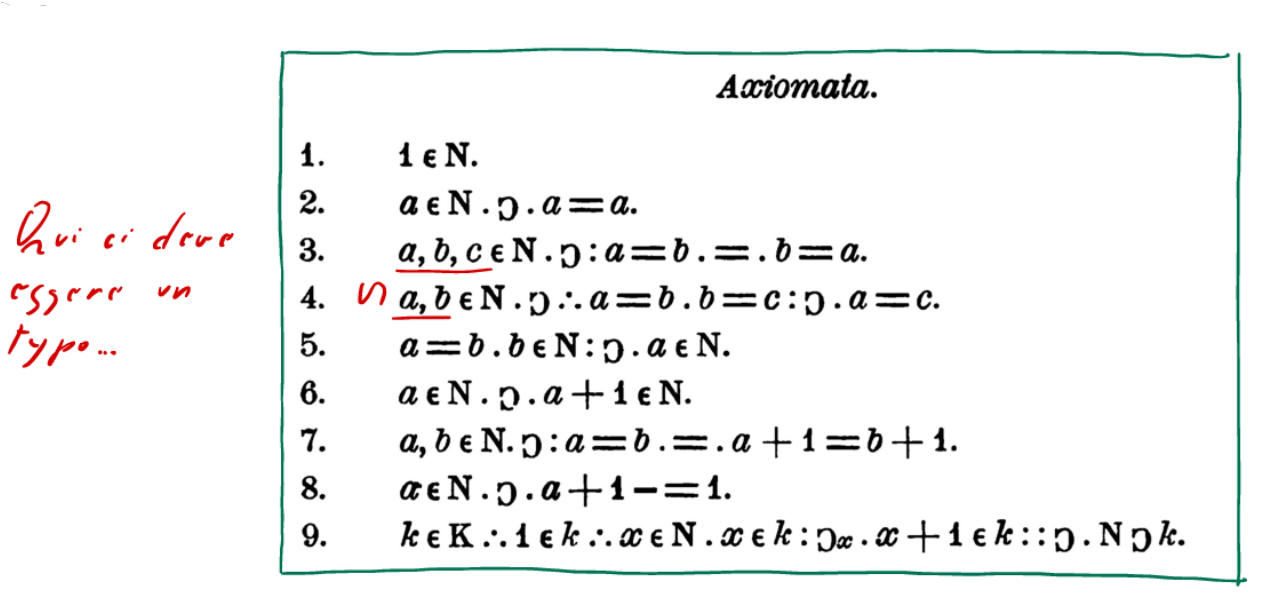
\includegraphics[width=10.5cm]{immagini/peano.png}
		\captionsetup{labelformat=empty}
		\caption{Apparivano così in ``\emph{Arithmetices principia}'', nel 1889, gli assiomi di Peano.}
\end{figure*}


\begin{theorem}[$\omega$ soddisfa gli assiomi di Peano]
	La funzione $\text{succ}: \omega \rightarrow \omega : n \mapsto s(n)$, è ben definita e $(\omega,\emptyset,\text{succ})$
	soddisfa gli assiomi di Peano.
\end{theorem}

\begin{proof}
	Prima di procedere con le verifiche controlliamo che la funzione $\text{succ} = s$ sia ben definita.
	Occorre assicurarsi che se $n \in \omega$, allora $\text{succ}(n) = s(n) \in \omega$. Fissiamo $n \in \omega$
	e consideriamo un qualunque insieme induttivo $A$. Siccome $A$ è induttivo $\omega \subseteq A$, quindi $n \in A$, e, di conseguenza $s(n) \in A$. Per 
	l'arbitrarietà di $A$, allora, $s(n)$ appartiene a ogni insieme induttivo (quindi all'intersezione, ovvero $\omega$).\\
	Dimostriamo ora che $\omega$ rispetta gli assiomi di Peano. Iniziamo con dimostrare (b) e (c), poi passeremo ad (a):
	\begin{enumerate}
		\item[(b)] Supponiamo, per assurdo, $s(n) = \emptyset$. Abbiamo allora che:
		\[ n \in s(n) =  n \cup \{n\} = s(n) = \emptyset
			\]
		contro la definizione di $\emptyset$.
		\item[(c)] Per verificare il principio di induzione, date le ipotesi, occorre verificare che il sottoinsieme di $\omega$ degli elementi per cui è vera $\Phi(n)$ è proprio tutto $\omega$, dunque 
		se dimostriamo che l'insieme $A = \{n \in \omega | \Phi(n)\} \subseteq \omega$ è induttivo, avendo gratis il primo contenimento, si ha $\omega = A$.
		\begin{enumerate}[(1)]
			\item Per ipotesi abbiamo che $\Phi(\emptyset)$, quindi $\emptyset \in A$.
			\item $n \in A \overset{\text{def. $A$}}{\implies} \Phi(n) \overset{\text{passo indutt.}}{\implies} \Phi(\text{succ}(n)) = \Phi(s(n)) \overset{\text{def. $A$}}{\implies} s(n) \in A$
		\end{enumerate}
		\item[(a)] La dimostrazione passa attraverso due lemmi.
					\begin{lemma}
					[Lemma 1]
					L'unione di un elemento di $\omega$ è contenuta nell'elemento: $\forall n \in \omega \; \bigcup n \subseteq n$.\footnote{E.g. $\bigcup 3 = \bigcup \{0,1,2\} = \{0,1\} = 2$.}
					\end{lemma}
					\begin{proof}
						Avendo dimostrato in (c) che in $\omega$ vale l'induzione possiamo usarla con $\Phi(n) \Mydef \bigcup n \subseteq n$. 
						\[
							\begin{split}
							\boxed{\Phi(\emptyset)} & \qquad \bigcup \emptyset = \emptyset \subseteq \emptyset \\
							\boxed{\Phi(n) \rightarrow \Phi(s(n))} & \qquad \bigcup s(n) = \bigcup(n \cup \{n\}) \overset{\star}{=} \underbrace{\left(\bigcup n\right)}_{\subseteq n} \cup n \overset{\text{Hp. indutt.}}{\subseteq} n \cup n = n \subseteq s(n)
							\end{split}
						\]
						(si noti che il passo base è coerente con le definizioni delle abbreviazioni date), e $\star$ vale in quanto:
						\[ \begin{split}
							x \in \bigcup(n \cup \{n\}) \overset{\text{def.}}{\iff} &\quad \exists y ( x \in y) \land (y \in (n \cup\{n\})) \\
														\overset{\text{caratt. $\cup$}}{\iff} &\quad \exists y( x \in y) \land (y \in n \lor y = n)\\
														\overset{\text{distrib. $\land$}}{\iff} &\quad \exists y \; ( x \in y \land y \in n) \lor (x \in y \land y = n)\\
														\iff &\quad \exists y ( x \in y \land y \in n) \lor \exists y(x \in y \land y = n)\\
														\overset{\text{def.}}{\iff} &\quad x \in \bigcup n \lor x \in n\\
														\overset{\text{caratt. $\cup$}}{\iff} &\quad x \in \left(\bigcup n\right) \cup n
						\end{split}
							\]
						(dove alla secondo membro della seconda equivalenza abbiamo che $y \in \{n\}$ e per \hyperref[ax2]{estensionalità} equivale a $y = n$.).
					\end{proof}
					\begin{lemma}
						[Lemma 2]
						L'unione dei successori di un elemento in $\omega$ è proprio l'elemento: $\forall n \in \omega \; \bigcup s(n) = n$.
					\end{lemma}
					\begin{proof}
						Ricopiando quanto fatto nel passo induttivo della dimostrazione precedente abbiamo:
						\[ \bigcup s(n) = \bigcup (n \cup \{n\}) = \left(\bigcup n\right) \cup n \overset{\star}{\subseteq} n
							\]
						dove in $\star$ abbiamo usato che $\bigcup n \subseteq n$, non per ipotesi induttiva (visto che non stiamo facendo alcuna induzione), ma stiamo usando direttamente il risultato del Lemma 1.
						Naturalmente vale anche che $n \subseteq \bigcup s(n)$ (ogni elemento di $n$ è elemento dell'elemento $n$ in $s(n)$), dunque vale la tesi.
					\end{proof}
					Finalmente abbiamo che, per il Lemma 2:
					\[ s(m) = s(n) \implies \bigcup s(m) = \bigcup s(n) \overset{\text{Lemma 2}}{\iff} m = n
						\]
					dove la prima freccia è data dal fatto che stiamo considerando l'unione di insiemi uguali, dunque succ$: \omega \rightarrow \omega$ è iniettiva.
	\end{enumerate}
\end{proof}

\subsection{L'ordine di omega}
Conviene, adesso, sviluppare un po' di tecnologia per manipolare i numeri interi. Dopo, dimostreremo altresì che gli assiomi di Peano hanno un unico modello $(\NN, 0, \text{succ})$
a meno di isomorfismi.

\begin{notation}[Relazione di ordine su $\omega$]
	Dati $m,n \in \omega$, scriviamo:
	\[ m < n \Mydef m \in n \footnote{Per essere precisi non stiamo usando $\in$ come una relazione (visto che abbiamo assunto all'inizio che fosse un simbolo del linguaggio della teoria degli insiemi),
	ma stiamo definendo $< \Mydef \{(m,n) \in \omega \times \omega | m \in n\}$. Inoltre se aggiungiamo la diagonale $\Delta_\omega$ a $<$, otteniamo $\leq$ (cioè $m \leq n \Mydef (m \in n) \lor (m = n)$), che, come visto, è legata alla corrispondente relazione d'ordine 
	stretto, e godrà di tutte le stesse proprietà (come vedremo man mano).}
		\]
\end{notation}

\begin{proposition}[Ordinamento totale di $\omega$]
	La relazione $<$ è un ordine totale su $\omega$. 
\end{proposition}

Per dimostrare questa proposizione, sono comodi alcuni lemmi.

\pagebreak

\begin{remark}[Successore del secondo termine in un'appartenenza]
	\label{succ2}
	Si osserva che valgono le seguenti cose:
	\begin{enumerate}[(1)]
		\item $m \in n \rightarrow m \in s(n)$, infatti $n \subseteq n \cup \{n\} = s(n)$ (banalmente se $m$ è contenuto in $n$ allora è contenuto anche nel suo successore).
		\item $m \in s(n) \rightarrow (m \in n \lor m = n)$, ciò se $m$ è nel successore di $n$, allora è $n$ stesso o un suo elemento, infatti:
		 \[ \begin{split}
			m \in s(n) = n \cup \{n\} & \iff m \in (n \cup \{n\}) \\
									& \iff (m \in n) \lor (m \in \{n\}) \\
									&\iff (m \in n) \lor (m = n)
		 \end{split}
			\]
		(nella seconda equivalenza si è usata la caratterizzazione data dell'appartenenza ad un unione di insiemi, e nella terza il fatto che se $m$ appartiene ad un singoletto, allora per \hyperref[ax2]{estensionalità} è proprio l'unico elemento del singoletto).
	\end{enumerate}
\end{remark}

\begin{lemma}[Successore del primo termine in un'appartenenza]
	$\forall a,b \in \omega \; a \in b \rightarrow (s(a) \in b \lor s(a) = b)$.\footnote{Moralmente: se un numero è strettamente più piccolo di un altro, o il suo successore è a sua volta più piccolo del secondo numero, o coincide con quest'ultimo.}
\end{lemma}

\begin{proof}
	Procediamo per induzione su $b$.
	\begin{itemize}
		\item[$\boxed{\text{caso $b = 0$}}$] $a \in \emptyset \rightarrow \ldots$ vera a vuoto, perché $a \in \emptyset$ è falsa (dunque l'implicazione è sempre vera, indipendentemente dal valore di verità dell'antecedente).
		\item[$\boxed{\text{caso $b = s(n)$}}$] L'ipotesi induttiva è $a \in n \rightarrow (s(a) \in n \lor s(a) = n)$. Dobbiamo dimostrare:
		\[ a \in s(n) \rightarrow (s(a) \in s(n) \lor s(a) = s(n))
			\]
		abbiamo che $a \in s(n) \iff a \in n \cup \{n\} \iff a \in n \lor a = n$. Quindi abbiamo due casi:
		\[ \begin{split}
			& a \in n \overset{\text{Hp. indutt.}}{\implies} (s(a) \in n) \lor (s(a) = n) \overset{\text{def. $s(n)$}}{\iff} s(a) \in s(n) \\
			& a = n \iff s(a) = s(n)
		\end{split}
			\]
		(la seconda equivalenza è giustificata dal fatto che abbiamo dimostrato che la funzione successore in $\omega$ è iniettiva).
	\end{itemize}
\end{proof}

Possiamo ora dimostrare la proposizione iniziale.

\begin{proof}
	Per verificare che $<$ è una relazione di ordine stretto totale, dobbiamo verificare che è irriflessiva, transitiva e totale (cioè presi qualsiasi due elementi di $\omega$ la loro coppia ordinata appartiene a $<$).
	\begin{itemize}
		\item[$\boxed{\text{transitività}}$] Vogliamo verificare che $(a \in b \land b \in c) \rightarrow a \in c$. Procediamo per induzione su $c$:
		\begin{itemize}
			\item[$\boxed{\text{caso $c = 0$}}$] la premessa $b \in c$ è falsa, quindi l'implicazione è vera a vuoto (l'antecedente è sempre falso, quindi l'implicazione sempre vera).
			\item[$\boxed{\text{caso $c = s(n)$}}$] assumiamo per ipotesi induttiva $(a \in b \land b \in n) \rightarrow a \in n$, e vogliamo dimostrare:
				\[ (a \in b \land b \in s(n)) \rightarrow a \in s(n)
					\]
				Osserviamo che $a \in b \implies a \in s(b)$, e che $b \in s(n) \overset{\text{Lemma}}{\implies} s(b) \in s(n) \lor s(b) = s(n)$, abbiamo quindi due casi in base a $s(b)$:
				\[ \begin{split}
					& s(b) = s(n) \implies a \in s(b) = s(n) \implies a \in s(n)\\
					& s(b) \in s(n) \implies a \in s(b) \in s(n) \implies a \in s(n)
				\end{split}
					\]
				questo usando il lemma precedente, potevamo anche scegliere di usare l'osservazione per dire che $b \in s(n) \implies b = n \lor b \in n$ e ottenere ancora i casi:
				\[  \begin{split}
					& b = n \implies a \in b = n \overset{\text{Oss.}}{\implies} a \in s(n) \\
					& b \in n \implies a \in b \in n \implies a \in n \overset{\text{Oss.}}{\implies} a \in s(n)
					\end{split}
					\]
		\end{itemize}
		\item[$\boxed{\text{irriflessività}}$] Vogliamo verificare $\neg \,a \in a$, e lo facciamo per induzione su $a$:
		\begin{itemize}
			\item[$\boxed{\text{caso $a = 0$}}$] $\neg \, \emptyset \in \emptyset$, vero per definizione di $\emptyset$.
			\item[$\boxed{\text{caso $a = s(n)$}}$] L'ipotesi induttiva è $\neg \, n \in n$, e vogliamo verificare che $\neg s(n) \in s(n)$. Procediamo per assurdo, supponiamo che $s(n) \in s(n)$, e per l'osservazione abbiamo due casi:
			\[ \begin{split}
				& s(n) = n \implies n \in n \; \lightning\\
				& s(n) \in n \implies n \in s(n) \in n \implies n \in n \; \lightning
			\end{split}
				\]
			($n \in n$ è falso perché per ipotesi induttiva $\neg(n \in n)$ è vero).
		\end{itemize}
		\item[$\boxed{\text{totalità}}$] Vogliamo dimostrare che $\forall a,b \in \omega (a \in b) \lor (a = b) \lor (b \in a)$. Iniziamo per induzione su $a$:
		\begin{itemize}
			\item[$\boxed{\text{caso $a = 0$}}$] La tesi diventa $\forall b \in \omega (\emptyset \in b) \lor (\emptyset = b) \lor (b \in \emptyset) \footnote{Ovviamente quest'ultimo caso è sempre faslo e quindi può essere escluso.}$. Procediamo quindi per induzione su $b$:
			\begin{itemize}
				\item \textbf{\underline{caso $b = 0$}} La tesi diventa $(\emptyset \in \emptyset) \lor (\emptyset = \emptyset)$, dove naturalmente la prima affermazione è sempre falsa, mentre la seconda è sempre vera, dunque la tesi è vera.
				\item \textbf{\underline{caso $b = s(m)$}} La tesi è $(\emptyset \in s(m)) \lor (\emptyset = s(m))$, con ipotesi induttiva $(\emptyset \in m) \lor (\emptyset = m)$. Abbiamo quindi due casi in base all'ipotesi induttiva:
				\[ \begin{split}
					& \emptyset \in m \implies \emptyset \in s(m) \\
					& \emptyset = m \implies \emptyset \in \{\emptyset\} = s(m)
				\end{split}
					\]
				in entrambi casi è vera la tesi perché è sempre vero il primo termine.
			\end{itemize}
			\item[$\boxed{\text{caso $a = s(n)$}}$] La tesi è $\forall b \in \omega (s(n) \in b) \lor (s(n) = b) \lor (b \in s(n))$, mentre l'ipotesi induttiva è $(n \in b) \lor (n = b) \lor (b \in n)$. Dall'ipotesi induttiva abbiamo quindi tre casi:
				\[ \begin{split}
					& n \in b \overset{\text{Lemma}}{\implies} s(n) \in b \lor s(n) = b \\
					& n = b \overset{\text{Iniett. del succ.}}{\implies} s(n) = s(b) \implies b \in s(b) = s(n) \implies b \in s(n)\\
					& b \in n \overset{\text{Oss.}}{\implies} b \in s(n) \implies b \in a 
				\end{split}
					\]
				in tutti e tre i casi almeno una delle tre proposizioni della tesi è vera, dunque la tesi è sempre vera.
		\end{itemize}
	\end{itemize}
\end{proof}

\begin{remark}[$\leq$ ordina totalmente $\omega$]
	Avendo dimostrato che $<$ è un ordine totale su $\omega$, abbiamo dimostrato in automatico che anche $\leq = < \cup \Delta$ lo è, infatti, per la corrispondenza tra i due (come si è visto precedentemente in una proposizione), anche le definizioni di ordine totale sono corrispondenti (in particolare per 
	$\leq$ ci basta che valga una tra $\leq$ e $\geq$, se valgono entrambe c'è l'=, mentre per $<$ chiedevamo nella definizione che valesse $<$, $>$ o $=$, quindi se nella dimostrazione precedente avessimo usato $\leq$ al posto di $<$ avremmo ottenuto lo stesso risultato perché le richieste nella definizione di ordine totale sono le stesse).
\end{remark}

\begin{corollary}[Rappresentazione dei numeri naturali]
	Un numero naturale è l'insieme dei numeri naturali minori di lui.
	\[ \forall m \in \omega \; m = \{n \in \omega | n < m\}
		\]
\end{corollary}

\begin{proof}
	Vogliamo dire che $m = \{ n \in \omega | n \in m\}$, ossia per definizione di sottoinsieme che $m \subseteq \omega$. Per induzione: $\emptyset \subseteq \omega$ è vera (perché $\omega$ è induttivo).
	Assumiamo che $m \subseteq \omega$, allora $s(m) = \underbrace{m}_{\subseteq \omega} \cup \{m\}$ e $\{m\} \subseteq \omega$ perché $m \in \omega$ per ipotesi iniziale, quindi si conclude che $s(m) \subseteq \omega$.
\end{proof}

\begin{corollary}[Più piccolo = contenuto]
	$\forall m,n \in \omega (m \leq n \leftrightarrow m \subseteq n$).\footnote{Naturalmente il lemma vale anche con $<$ e $\subsetneq$.}
\end{corollary}

\begin{proof}
	Siccome $\omega$ è totalmente ordinato, si danno due casi (nel primo dimostro $\rightarrow$, nel secondo dimostro che la negazione della premessa implica la negazione della conseguenza, che è equivalente [via contronominale] a $\leftarrow$):
	\begin{align*}
		& m \leq n \implies \forall x \in \omega (x < m \rightarrow x < n) \overset{\text{def. $<$}}{\implies} \forall x \in \omega (x \in m \rightarrow x \in n) \overset{\text{def. $\subseteq$}}{\implies} m \subseteq n \\
	    & n < m \implies n \in m \; \text{tuttavia} \; n \not\in n \; \text{quindi non può essere che $m \subseteq n$ ovvero} \; m \not\subseteq n
	\end{align*}
	($n \not \in n$ perché abbiamo dimostrato che $<$ è di ordine stretto su $\omega$, quindi irriflessiva, inoltre, nella dimostrazione del primo caso, si osserva che nel secondo passaggio è
	indifferente usare $<$ o $\leq$ nell'enunciato e dimostrazione del corollario\footnote{Mamino li mischia, ma valgono entrambi gli enunciati e le dimostrazioni.}.
\end{proof}
\pagebreak
\subsection{Induzione forte e principio del minimo}
\begin{theorem}
	[Principio di induzione - forma forte]
	Data una formula insiemistica $\Phi(x)$, vale:
	\[ (\forall n \in \omega (\forall x < n \; \Phi (x)) \rightarrow \Phi(n)) \rightarrow \forall n \in \omega \; \Phi(n)
		\]
	ovvero, se assumendo $\Phi(x)$ per tutti gli $x < n$, abbiamo $\Phi(n)$, allora $\Phi(n)$ è vera per tutti i numeri $n$.
\end{theorem}

\begin{remark}
	Chiaramente questa forma è ``forte'' perché permette di assumere un'ipotesi induttiva più forte dell'induzione di Peano. In quella, infatti, si deve dedurre $\Phi(n)$ a 
	partire da $\Phi$ del numero precedente. Qui, invece, possiamo far conto di sapere $\Phi$, non solo per il precedente, ma per tutti i numeri minori di $n$.
\end{remark}

\begin{proof}
	Definiamo $\psi(m) \Mydef \forall x < m \; \Phi(x)$ e dimostriamo per induzione debole che $\forall m \in \omega \; \psi(m)$, \textcolor{MidnightBlue}{ cioè che per ogni fissato naturale $\Phi$ è vera per i naturali più piccoli},
	in tal modo, per ogni $n \in \omega$ sappiamo che è vera $\psi(n+1) \implies \Phi(n)$, che è proprio la tesi.
	\begin{itemize}
		\item[$\boxed{m = 0}$] Abbiamo che $\psi(0) = \forall x < 0 \; \Phi(x) \equiv \forall x (x < 0 \to \Phi(x))$, che è vera a vuoto in quanto $x < 0 \equiv x \in \emptyset$ che è sempre falso, dunque l'implicazione tra partentesi è sempre vera.
		\item[$\boxed{m \implies m + 1}$] Assumiamo che $\psi(m) = \forall x < m \; \Phi(x)$ sia vera e mostriamo che $\psi(m) = \forall x < m + 1 \; \Phi(x)$ è vera. Per un lemma visto $x < s(m) \implies x < m \lor x = m$, nel primo caso $\Phi(x)$ è vera per ipotesi induttiva.
		Nel caso di $\Phi(m)$, abbiamo per ipotesi che \textcolor{purple}{$\forall n \in \omega (\forall x < n \; \Phi (x)) \rightarrow \Phi(n)$}, dunque, per $n = m$, abbiamo visto nel primo caso che $\forall x < m \; \Phi(m)$, per cui l'ipotesi (vera) ha antecedente vero, che ci dà necessariamente conseguente $\Phi(m)$ vero.
	\end{itemize}
\end{proof}

\begin{theorem}
	[Principio del minimo]
	Sia $A \subseteq \omega$. Se $A \ne \emptyset$ allora esiste $n \in A$ tale che $\forall x \in A \; n \leq x$. Ovvero, ogni sottoinsieme non vuoto di $\omega$ ha un minimo elemento.
\end{theorem}

\textcolor{MidnightBlue}{\underline{Possibile idea di dimostrazione}: dimostriamo per induzione forte che se $n \in A$ - che è equivalente a $A\subseteq \omega \land A \ne \emptyset$ -, allora $A$ ha un minimo. Per ipotesi induttiva assumiamo che $\forall x < n \; x \in A \to A$ ha minimo, e dimostriamo che se $n \in A$, allora 
$A$ ha minimo. Dato $n \in A$, se esiste $x \in n$ tale che $x \in A$, allora $A$ ha minimo per ipotesi induttiva, altrimenti, se $\forall x < n \; x \not \in A$, allora $n$ è il minimo di $A$.}

\begin{proof}
	Dimostriamo la contronominale della tesi, ovvero se $A \subseteq \omega$ non ha un elemento minimo, allora $A$ è vuoto, cioè $\forall n \in \omega \; n \not \in A$. Procediamo per induzione forte, assumendo per ipotesi induttiva che $\forall x < n \; x \not \in A$, mostriamo che $n \not \in A$.
	Più precisamente vogliamo dimostrare che $(\forall x < n \; x \not \in A) \to n \not \in A$, ma ciò è equivalente al fatto che $A$ non abbia un minimo:
	\begin{align*}
		(\forall x < n \; x \not \in A) \to n \not \in A &\iff \neg(\exists x < n \; x \in A) \to n \not \in A \\
														 &\iff n \in A \to \exists x < n \; x \in A &&\text{(contronominale)}\\
														 &\iff \text{$A$ non ha minimo}
	\end{align*}
	abbiamo quindi dimostrato che l'implicazione che vogliamo dimostrare è equivalente all'ipotesi per cui è vera, inoltre per l'ipotesi induttiva l'antecedente dell'implicazione è vero, per cui, dalla tavola di verità,
	l'unica possibilità è che anche il conseguente $n \not \in A$ sia vero. Ciò verifica il passo induttivo e quindi l'induzione forte ci garantisce la contronominale della tesi - che naturalmente è equivalente a quest'ultima -.
\end{proof}

\begin{remark}
	Per completare l'equivalenza tra induzione, induzione forte e principio del minimo, andrebbe dimostrato anche che principio del minimo$\implies$induzione.
\end{remark}

\begin{definition}[Insieme ben ordinato]
	Un insieme totalmente ordinato $(S, <)$ si dice \vocab{bene ordinato} se ogni sottoinsieme non vuoto ha un minimo.\footnote{Cioè se vale il principio del minimo c(come vale in $\omega$).}
	\[ \forall A \subseteq S \; A \ne \emptyset \rightarrow \exists m \in A \; \forall x \in A \; m \leq x
		\]
\end{definition}

La nozione di buon ordine è stata introdotta da Cantor agli albori della teoria degli insiemi, e giocherà un ruolo centrale in questo corso.

\begin{example}
	$(\omega, <)$ è un insieme bene ordinato\footnote{Si usa la notazione di coppia ordinata per indicare sia l'insieme sia la relazione che c'è sopra.} per quanto visto nel teorema precedente.
\end{example}

\begin{exercise}
	Dimostra che $X = s(s(s(\omega)))$ è bene ordinato dalla relazione $a < b \Mydef a \in b$.
\end{exercise}

\begin{soln}
	Dato $(\omega,<)$, basta considerare la seguente relazione:
	\[ \prec := < \cup (\omega \times \{\omega\}) \cup (s(\omega) \times \{s(\omega)\}) \cup (s(s(\omega)) \times \{s(s(\omega))\})\,\footnote{Che formalmente è un sottoinsieme di $s(s(s(\omega))) \times s(s(s(\omega)))$.}
		\]
	dove $(x,y) \in \prec \leftrightarrow x \in y$. Si vede quindi che $(s(s(s(\omega))),\prec)$ è un ordine totale (fondamentalmente perché $<$ lo è, 
	e le coppie che abbiamo aggiunto sono costruite apposta per rispettare la definizione di ordine [stretto] totale). Abbiamo costruito $\prec$ in modo che 
	$\forall n \in \omega \; n \prec \omega$, inoltre vale anche [per costruzione] che $\omega \prec s(\omega) \prec s(s(\omega))$, dunque, dato $S \subseteq s(s(s(\omega)))$,
	se $S \cap \omega \ne \emptyset$, allora il minimo esiste ed è dato da $\min_<(S \cap \omega)$. Se $S \cap \omega = \emptyset$ (ovvero se $S$ è un sottoinsieme di $\{\omega,s(\omega),s(s(\omega))\}$),
	allora per definizione di $\prec$ (come scritto sopra), per tutti i sottoinsiemi possibili abbiamo sempre un minimo [per la totalità di $\prec$]. Pertanto $\forall S \subseteq s(s(s(\omega)))$ c'è un minimo
	e quindi in $s(s(s(\omega)))$ vale il principio del minimo, cioè è ben ordinato.
\end{soln}

\subsection{Ricorsione numerabile}
La ricorsione è il procedimento per cui si costruisce una funzione $f : \omega \rightarrow \text{qualcosa}$, definendo $f(s(n))$ a partire da $f(n)$, o,
più in generale da $f(\emptyset),\ldots,f(n)$. Questo è un procedimento fondamentale: potremmo dire che è IL modo di pensare gli infidi puntini ($\ldots$). Vediamo qualche esempio.

\begin{example}
	[Operazioni aritmetiche]
	Possiamo definire somma e prodotto come:
	\[ \begin{cases}
		a + \textcolor{red}{0} = a \\
		a + \textcolor{red}{s(b)} = s(a + b)
	\end{cases}
	\qquad
	\begin{cases}
		a \cdot \textcolor{red}{0} = 0\\
		a \cdot \textcolor{red}{s(b)} = a \cdot b + a
	\end{cases}
		\]
	anziché $a + b = \underbrace{s(s(\ldots a \ldots))}_{\text{$b$ successori}}$ (abbiamo il caso base con 0, e poi si procede ricorsivamente dal caso base fino a $b$) e $a \cdot b = \underbrace{a + a + \ldots + a}_{\text{$b$ volte}}$ (ricorsivamente ad un certo 
	punto si partirà da $a$ e si inizierà a sommare).
\end{example}

\begin{example}
	[Potenza e fattoriale]
	Possiamo definire ricorsivamente potenze e fattoriali come segue:
	\[ \begin{cases}
		a^{\textcolor{red}{0}} = 1\\
		a^{\textcolor{red}{s(b)}} = a^b \cdot a
	\end{cases}
	\qquad
	\begin{cases}
		\textcolor{red}{0}! = 1\\
		\textcolor{red}{s(a)}! = a! \cdot s(a)
	\end{cases}
		\]
	anziché $a^b = \underbrace{a \cdot a \cdot \ldots \cdot a}_{\text{$b$ volte}}$ e $a! = 1 \cdot 2 \cdot \ldots \cdot (a - 1) \cdot a$.
\end{example}

\begin{example}
	[Sommatoria]
	Possiamo definire la sommatoria come:
	\[\begin{cases}
		\displaystyle
		\sum_{i = 0}^{\textcolor{red}{0}} f(i) = 0\\
		\displaystyle
		\sum_{i = 0}^{\textcolor{red}{s(a)}} f(i) = \left(\sum_{i=0}^{a} f(i) \right) + f(s(a))
	\end{cases}
		\]
	anziché $\displaystyle\sum_{i = 0}^a f(i) = f(0) + f(1) + \ldots + f(a)$ (cioè con la sommatoria definita ricorsivamente stiamo eliminando il fastidioso discorso (poco formale) dei puntini \dots).
\end{example}

Altre \vocab{successioni} - \textbf{ossia funzioni con dominio $\omega$} - sono definite nella maniera più naturale proprio per ricorsione.

\begin{example}[Esempio di applicazione della ricorsione]
	In quanti modi posso coprire una sequenza di $n$ caselle $\underbrace{\square\square\square\ldots\square\square}_{n}$ con tessere di una o due caselle,
	$\square$ e $\square\square$, che non si sovrappongano e non lascino caselle scoperte?
\end{example}

\begin{soln}
	Detto $F_n$ il numero di ricoprimenti di una sequenza lunga $n$, vediamo che la tessera più a sinistra può essere $\square$ o $\square \square$. Nel primo caso, ci sono 
	$F_{n-1}$ modi di completare il ricoprimento, nel secondo caso $F_{n-2}$. Abbiamo quindi trovato una relazione ricorsiva del numero di ricoprimenti in funzione di $n$:
	\[ F_n = F_{n-1} + F_{n-2}\footnote{Cioè il numero totale di modi di ricoprire la sequenza di $n$ caselle deriva dalla somma dei due casi, che rappresentano i modi di ricoprire le altre caselle fissata quella/e iniziale/i, ciò fissati i casi base ci definisce bene (via ricorsione numerabile) una successione che conta il numero 
	di ricoprimenti in funzione di $n$.}
		\]
	La sequenza risulta completamente determinata, per ricorsione, osservando che $F_0 = F_1 = 1$: sono i \vocab{numeri di Fibonacci}.
\end{soln}

\textbf{In un certo senso, induzione e ricorsione sono due facce della stessa medaglia}: dove l'induzione dimostra $\Phi(s(n))$ assumendo di sapere 
$\Phi(n)$, la ricorsione calcola $f(s(n))$ assumendo di sapere $f(n)$. Lo stesso parallelismo, vedremo, si presenterà per l'induzione e la ricorsione transfinita.
Tornando al numerabile: come abbiamo enunciato due forme dell'induzione, enunceremo due forme della ricorsione.\\
La semplice osservazione che segue dice che due funzioni sono uguali precisamente quando assumono gli stessi valori.

\begin{remark}
	[Estensionalità per funzioni]
	Date $f,g : A \rightarrow B$, allora:
	\[ f = g \leftrightarrow \forall x \in A \; f(x) = g(x)
		\]
	(dove l'uguaglianza di funzioni non è altro che uguaglianza di sottoinsiemi in $A \times B$).
\end{remark}

\begin{proof}
	Si osserva che:
	\[ (x,y) \in f \overset{\text{def. $f$}}{\iff} y = f(x) \overset{\text{Hp.}}{\iff} y = g(x) \overset{\text{def. $g$}}{\iff} (x,y) \in g
		\]
	e si conclude per \hyperref[ax2]{estensionalità} che quanto scritto sopra equivale a dire che gli insiemi $f$ e $g$ sono uguali.
\end{proof}

\begin{notation}[Insieme delle funzioni da $A$ a $B$]
	Indichiamo con ${}^{A}B$ l'insieme delle funzioni da $A$ a $B$, che esiste per \hyperref[ax3]{separazione} in $\ps(A \times B)$.
\end{notation}

\begin{theorem}
	[Ricorsione numerabile - prima forma]
	\label{ric1}
	Dato un insieme $A$, un elemento $k \in A$ e una funzione:
	\[ h : \omega \times A \rightarrow A
		\]
	esiste un'unica funzione $f : \omega \rightarrow A$ tale che:
	\[ f(0) = k \quad \land \quad \forall n \in \omega\; f(s(n)) = h(n,f(n))
		\]
\end{theorem}

\begin{example}[Potenza e fattoriale con la ricorsione numerabile]
	Per definire $a^b$ considero $k = 1$, $h(n,x) = a \cdot x$, e $h(0,x) = k = 1$. Per definire il fattoriale $k = 1$, $h(n,x) = s(n) \cdot x$ e $h(0,x) = k = 1$.
\end{example}

\begin{exercise}
	Come potrei costruire $F_n$ usando questo teorema?
\end{exercise}

\textcolor{MidnightBlue}{Il piano consiste nel trovare una formula $\Phi(x,y)$ che dice ``$y = f(x)$'' - questa è la vera difficoltà 
della dimostrazione - poi semplicemente otteniamo $f$ per separazione nell'insieme $\omega \times A$ (in tal modo $f$ è una funzione da $\omega$ ad $A$) usando la formula $\Phi$.
Dire ``$y = f(x)$'' vuol dire ``i primi $x$ passaggi della ricorsione, partendo da $k$, conducono a $y$''.}

\begin{proof}
	Dato $x \in \omega$ diciamo che $g$ è una \vocab{$x$-approssimazione} - per la $h$ fissata nell'ipotesi - se la vale:
	\[ \text{$g$ $x$-approssimazione} \Mydef \begin{cases}
		g \in {}^{s(x)}A \\
		g(0) = k \\
		\forall n \in x\; g(s(n)) = h(n,g(n))
	\end{cases}
		\]
	di fatto $g$ è la ricorsione che stiamo cercando di definire, date le ipotesi, fatta un numero finito di passi - $x \in \omega$ -.
	Iniziamo a dimostrare quindi che questa ricorsione finita esiste per ogni numero finito di iterazioni $x \in \omega$ fissato.\\
	\textcolor{MidnightBlue}{Il vantaggio di tagliuzzare $f$ in $x$-approssimazioni è che così otteniamo un parametro, $x$, su cui impostare un'induzione.}	
	\begin{lemma}[Esistenza e unicità delle $x$-approssimazioni in $\omega$]
		$\forall x \in \omega$, fissata $h$ come nelle ipotesi del teorema di ricorsione, $\exists ! \, g$ ``$g$ è una $x$-approssimazione per $h$''.
	\end{lemma}

	\begin{proof}
		Fissato $x \in \omega$, possiamo procedere per induzione - di fatto sul numero di iterazioni della ricorsione -.
		\begin{itemize}
			\item[$\boxed{x = 0}$] Basta osservare che l'unica $0$-approssimazione è la funzione $\{(0,k)\}$. Infatti il dominio
			è $\{0\}$ per definizione, $g(0) = k$, e vale a vuoto la terza condizione, l'unicità è banale, pertanto l'unica $0$-approssimazione possibile per $h$ è proprio la funzione $g = \{(0,k)\}$.
			\item[$\boxed{x = s(a)}$] Per ipotesi induttiva abbiamo che esiste ed è unica una $a$-approssimazione per $h$, diciamo $g$, vogliamo dimostrare che esiste ed è unica una $s(a)$-approssimazione per $h$.
			Per ipotesi $g \in {}^{s(a)} A$, $g(0) = k$ e $\forall b \in a \; g(s(b)) = h(b,g(b))$, possiamo quindi estendere $g$ a $s(a)$ come segue:
			\[ g' = g \cup \{(s(a), h(a,g(a)))\}
				\]
			A questo punto è immediato verificare che $g'$ è una $s(a)$-approssimazione, infatti, $\Dom(g') = \Dom(g) \cup \{s(a)\} = s(a) \cup \{s(a)\} = s(s(a))$, $g'(0) = g(0) = k$ e $\forall t \in a\; g'(s(t)) = g(s(t)) = h(t,g(t))$,
			e per costruzione, $g'(s(a)) = h(a,g(a))$. Per l'unicità, sappiamo per ipotesi induttiva che esiste un'unica $a$-approssimazione per $h$, quindi, date $g'$ e $g''$ due $s(a)$-approssimazioni per $h$, si ha necessariamente che $g_{|s(a)}' = g_{|s(a)}''$,
			e in particolare ciò significa che $g'(a) = g''(a)$, da cui:
			\[ g'(s(a)) \overset{\text{def.}}{=} h(a,g'(a)) \overset{\text{Hp. indutt.}}{=} h(a,g''(a)) \overset{\text{def.}}{=} g''(s(a))
				\]
		\end{itemize}	
	\end{proof}
	Il lemma appena dimostrato ci garantisce esistenza e unicità di funzioni ricorsive finite - di lunghezza arbitraria fissata - che rispettano le stesse proprietà di $f$ nella tesi (ad eccezione del dominio naturalmente), vogliamo ora far vedere che esiste una funzione con tali proprietà con dominio tutto $\omega$.
	Introduciamo la formula $\Phi$:
	\[ \Phi(x,y) \Mydef \exists g \in {}^{s(x)}A \; \text{``tale che $g$ è una $x$-approssimazione''} \land\, g(x) = y
		\]
	Per l'unicità delle $x$-approssimazioni possiamo scrivere $\forall x \in \omega \; \exists \textcolor{red}{!}\, y \; \Phi(x,y)$. Possiamo quindi finalmente definire $f$ per separazione in $\omega \times A$:
	\[ f := \{(x,y) \in \omega \times A | \Phi(x,y)\}\footnote{Di fatto stiamo costruendo $f$ con le ricorsioni finite - cioè $f$ manda $x$ nell'unico $y$ raggiungibile iterando la ricorsione $x$ volte, in altre parole è la successione delle ricorsioni troncate -, che però ora sappiamo ci sono e sono uniche qualsiasi sia la lunghezza - quindi per infiniti valori di $x \in \omega$ -.}
		\]
	L'unicità di $y$ osservata prima ci garantisce che $f$ è una funzione, occorre dunque verificare che soddisfi le proprietà richieste nella tesi.
	\begin{itemize}
		\item[$\boxed{f(0) = k}$] Abbiamo visto che esiste un'unica 0-approssimazione, $g = \{(0,k)\}$, e per definizione di $f$, abbiamo proprio che $f(0) = g(0) = k$.
		\item[$\boxed{f(s(n)) = h(n,f(n))}$] Segue per costruzione di $f$ che $f(s(n)) = g(s(n))$, con $g \in {}^{s(s(n))}A$ che è una $s(n)$-approssimazione, pertanto, $g(s(n)) = h(n,g(n))$,
		ora $g(n) = g_{|s(n)}(n)$ è una (l'unica) $n$-approssimazione per $h$ (lo si verifica facilmente), per cui, per definizione di $f$, $f(n) = g(n)$ e rimettendo tutto assieme si ottiene:
		\[ f(s(n)) = g(s(n)) = h(n,g(n)) = h(n,f(n))
			\]
	\end{itemize}
	Ciò dimostra che una $f$ ottenuta per separazione soddisfa la tesi del teorema di ricorsione numerabile.
	L'unicità di $f$ segue facilmente per induzione, Date $f'$ e $f''$ che soddisfano la ricorsione abbiamo:
	\[ f'(0) = k = f''(0) \qquad f'(s(n)) = h(n,f'(n)) \overset{\text{Hp. indutt.}}{=} h(n,f''(n)) = f''(s(n))
		\]
	e per estensionalità di funzioni si conclude che $f' = f''$.
\end{proof}

Procedendo come negli esempi all'inizio di questa sezione, il \hyperref[ric1]{teorema di ricorsione numerabile} ci consente di costruire le operazioni aritmetiche, le potenze, etc.
A titolo di esempio, vediamo nel dettaglio, il caso della somma.

\begin{example}
	[Costruzione di $+ : \omega \times \omega \rightarrow \omega$]
	Vogliamo formalizzare la definizione:
	\[ \begin{cases}
		a + \textcolor{red}{0} = 0\\
		a + \textcolor{red}{s(b)} = s(a+b)
	\end{cases}
		\]
	Per il \hyperref[ric1]{teorema di ricorsione numerabile} sappiamo che, per ogni $a \in \omega$ fissato, esiste un'unica $f : \omega \rightarrow \omega$ tale che:
	\[ f(\textcolor{red}{0}) = a \land \forall b \in \omega \; f(\textcolor{red}{s(b)}) = s(f(b))
		\]
	Scriviamo quindi:
	\[ a + x = y \Mydef \exists f \in {}^{\omega}\omega \;\; f(0) = a \; \land  \; f(x) = y \; \land \; \forall b \in \omega \; f(s(b)) = s(f(b))
		\]
\end{example}

L'applicazione che segue chiude il conto che abbiamo lasciato aperto con gli assiomi di Peano. Dimostriamo che essi identificano un'unica struttura a meno di isomorfismi, quindi $\omega$ è 
a buon diritto, l'insieme dei numeri naturali.

\begin{theorem}[Unicità dei numeri naturali]
	Supponiamo che $(\NN, 0, \text{succ})$ soddisfi gli assiomi di Peano, allora $(\NN, 0, \text{succ})$ \textbf{e} $(\omega,\emptyset,s)$ sono strutture isomorfe - \textbf{ossia, formalmente, esiste}:
	$ f : \omega \rightarrow \NN$ \textbf{bigettiva} tale che:\footnote{Cioè gli assiomi di Peano hanno un unico modello a meno di isomorfismo di strutture.}
	\begin{enumerate}[(i)]
		\item $f(\emptyset) = 0$.
		\item $\forall n \in \omega \; f(s(n)) = \text{succ}(f(n))$.
	\end{enumerate}
\end{theorem}

Fa comodo isolare la seguente osservazione.

\begin{remark}[Ogni numero in $\omega\setminus\emptyset$ è successore]
	$\forall x \in \omega \; x \ne 0 \rightarrow \exists y \in \omega \; x = s(y)$, ovvero ogni numero diverso da 0 è il successore di qualcos'altro.
\end{remark}

\begin{proof}
	Induzione su $x$. Il caso $x = 0$ è vero a vuoto (essendo la premessa sempre automaticamente falsa). Nel caso $x = s(m)$ basta prendere $y = m$ e si ha $x = s(y)$.
\end{proof}

\begin{proof}
	Per il \hyperref[ric1]{teorema di ricorsione} (stiamo prendendo $A = \NN$, e $k = 0$ e $h = \text{succ}$) c'è un'unica $f$ che soddisfa le condizioni $f(\emptyset) = 0$ e $\forall n \in \omega \; f(s(n)) = \text{succ}(f(n))$.
	Resta da constatare che $f$ è bigettiva.
	\begin{itemize}
		\item[\boxed{\text{Surgettività}}] Per ipotesi $(\NN, 0, \text{succ})$ soddisfa gl assiomi di Peano, per cui vale il principio di induzione. Dimostriamo quindi per induzione in $(\NN, 0, \text{succ})$ la surgettività di $f$.
		\begin{itemize}
			\item[$\boxed{y = 0}$] Basta osservare che $f(\emptyset) = 0$ per costruzione.
			\item[$\boxed{y = \text{succ}(n)}$] Per ipotesi induttiva esiste $x \in \omega$ tale che $f(x) = n$, da cui si ottiene, per definizione di $f$ che $f(s(x)) = \text{succ}(n)$.
		\end{itemize}
		\item[\boxed{\text{Iniettività}}] Per assurdo supponiamo ci sia un elemento in $\omega$ con la stessa immagine di un altro. Sia $x :=\min\{n \in \omega | \exists y \in \omega \; f(n) = f(y)\}$, dunque, per minimalità di $x$, esiste $y \in \omega$ con $y > x$, tale per cui $f(x) = f(y)$.
		Poiché $y > x$ si ha che $y > 0$, per cui $y = s(y')$ per qualche $y' \in \omega$, distinguiamo quindi due casi.
		\begin{itemize}
			\item[$\boxed{x = 0}$] In tal caso si deve avere che:
			\[
				\text{succ}(f(y')) \overset{\text{def. $f$}}{=} f(s(y'))
								   \overset{y = s(y')}{=} f(y)
								   \overset{\text{Hp. assurda}}{=} f(x) \overset{\text{def. $f$}}{=} 0
				\]
			per cui $0$ è successore di qualcosa in $\NN$, che è contro gli assiomi di Peano.
			\item[$\boxed{x \ne 0}$] Per l'osservazione possiamo scrivere $x = s(x')$, da cui:
			\[ \text{succ}(f(x')) \overset{\text{def. $f$}}{=} f(s(x')) = f(x) \overset{\text{Hp. assurda}}{=} f(y) = f(s(y')) \overset{\text{def. $f$}}{=} \text{succ}(f(y'))
				\]
			e dagli assiomi di Peano in $\NN$, per l'iniettività del successore, si ha $f(x') = f(y')$, con $x' < x$, per cui contro la minimalità di $x \; \textcolor{red}\lightning$.
		\end{itemize}
	\end{itemize}
\end{proof}

Se, infine, volgiamo la nostra attenzione all'esempio dei numeri di Fibonacci, vediamo che non è possibile definire questa sequenza applicando il \hyperref[ric1]{teorema di ricorsione}
in maniera diretta, perché $F_n$ non dispense solo dal termine precedente della sequenza, $F_{n-1}$, ma anche da $F_{n-2}$. Ce la si potrebbe cavare con un trucco, per esempio definendo la funzione
$n \mapsto (F_n,F_{n+1})$ da $\omega$ a $\omega \times \omega$. È comodo, però, disporre di una versione più versatile del teorema di ricorsione numerabile.

\begin{theorem}
	[Ricorsione numerabile - seconda forma]
	Dato un insieme $A$, denotiamo con $A^*$ il sottoinsieme delle funzioni con dominio un naturale, $A^* = \bigcup_{n \in \omega} {}^n A$.
	Sia $h : A^* \rightarrow A$, allora esiste un'unica funzione
	$f: \omega \rightarrow A$ tale che:
	\[ \forall n \in \omega \; f(n) = h(f_{|n})\,\footnote{In altre parole $f(n)$ può dipendere in maniera arbitraria dai valori assunti da $f$ su $n$, dove tale arbitrarietà è stabilità da $h$, la 
	quale valuta una funzione, definita su un dominio finito, su alcuni suoi fissati - in funzione di $n$ - valori.}
		\]
\end{theorem}

\textcolor{MidnightBlue}{L'idea è di definire, mediante la prima forma del \hyperref[ric1]{teorema di ricorsione}, la successione della troncata di $f$, ossia la funzione $f' : n \mapsto f_{|n}$, e da questa definire poi la $f$ voluta - un modo alternativo, sarebbe 
ripetere la dimostrazione della prima forma -.}

\begin{proof}
	Definiamo per \hyperref[ric1]{ricorsione numerabile v.1} la successione delle ricorsioni date da $h$ troncate al valore $n$ - cioè $f'(s(n))$ è la funzione che fa la ricorsione determinata da $h$ fino ad $n$ -:
	\[ f' : \omega \to \textcolor{purple}{A^*} : \begin{cases}
		f'(0) = 0 \\
		f'(s(n)) = f'(n) \cup \{(n,h(f'(n)))\}
	\end{cases}
		\]
	che appunto esiste ed è unica per il teorema di ricorsione numerabile ed è la successione delle (funzioni) troncate della funzione che vogliamo costruire. \\
	Definiamo ora $f(n) := (f'(s(n)))(n) = h(f'(n))$ \textcolor{MidnightBlue}{- cioè $f$ calcolata al valore $n$-esimo è data dal valore della $n+1$-esima troncata della ricorsione determinata da $h$, calcolata in $n$ -}, in tal modo abbiamo che $f : \omega \to A$ esiste ed è unica (come conseguenza dell'esistenza e dell'unicità di $f'$), pertanto non ci resta altro che verificare per induzione
	che effettivamente $f'$ sia la successione della troncata di $f$, cioè $\forall n \in \omega \; \textcolor{purple}{f_{|n} = f'(n)} \in A^*$ - in tal modo $h(f'(n)) = h(f_{|n})$ -.
	\begin{itemize}
		\item[$\boxed{n = 0}$] In tal caso si vede subito che $f_{|0} = \emptyset$, infatti qualsiasi funzione ristretta al vuoto dà il vuoto, d'altra parte, per costruzione, si ha anche che $f'(0) = 0$.
		\item[$\boxed{n = s(m)}$] Per ipotesi induttiva $f_{|m} = f'(m)$, vogliamo verificare che $f_{|s(m)} = f'(s(m))$:
		\begin{align*}
			f_{|s(m)} &= f_{|m} \cup \{(m,f(m))\} &&\text{(def. funzione)}\\
					  &= f'(m) \cup \{(m,f'(s(m))(m))\} &&\text{(Hp. indutt. + def. $f$)}\\
					  &= f'(m) \cup \{(m,h(f'(m)))\} = f'(s(m)) &&\text{(def. $f'$)}
		\end{align*}
	\end{itemize}
	Infine, quindi, $f(n) \overset{\text{def. $f$}}{=} f'(s(n))(n) \overset{\text{def. $f'$}}{=} h(f'(n)) \overset{\text{appena visto}}{=} h(f_{|n})$.
\end{proof}

\begin{example}
	[Esempio di applicazione]
	Per costruire la successione di Fibonacci, definiamo $h(g)$ in questo modo. Sia $n = \Dom(g)$. Se $n = \emptyset$ o $n = 1$, allora $h(g) = 1$.
	Altrimenti esistono $n-1, n-2 \in \omega$ tali che $s(n-1) = s(s(n-2)) = n$. Definiamo quindi $h(g) = g(n-1) + g(n-2)$\footnote{Abbiamo quindi ottenuto $h$ come funzione di funzioni con dominio in $\omega$ e in particolare più piccolo di $n$, dunque per il teorema tale $h$ definisce univocamente $f(n)$, a partire da $f_{|n} \in A^*$.}.
\end{example}

Abbiamo ora terminato di dimostrare le proprietà di base dei numeri naturali. Da qui, prende le mosse il corso di aritmetica. Nella prossima sezione, inizieremo
lo studio di un concetto squisitamente insiemistico: la cardinalità.

\begin{exercise}
	Dimostra commutatività, associatività, etc. di $+$ e $\cdot$.
\end{exercise}
\include{sezioni/Cardinalità}
\include{sezioni/Cardinalità finite}
\include{sezioni/Cardinalità del numerabile}
\include{sezioni/Cardinalità del continuo}
\section*{Stato del corso}
\addcontentsline{toc}{section}{Stato del corso}
È un dato di fatto - il primo teorema di incompletezza di Gödel - che ogni teoria \vocab{calcolabile} - i cui assiomi possano, cioè, essere elencati 
in maniera meccanica - è necessariamente incompleta. L'incompletezza non è quindi un difetto, o meglio, che lo sia oppure no è irrilevante, perché 
non può essere evitata.\\
Tuttavia, gli assiomi che abbiamo introdotto fino ad ora lasciano aperte lacune che sarebbe desiderabile colmare.

\begin{enumerate}[1.]
	\item Sarebbe ragionevole che questi insiemi esistessero [all'interno della teoria che stiamo costruendo]:
	\[ \{\emptyset, \{\emptyset\}, \{\{\emptyset\}\}, \{\{\{\emptyset\}\}\}, \ldots\}
		\]\[ \{\omega, s(\omega), s(s(\omega)), s(s(s(\omega))),\ldots\}
			\]
	Però gli assiomi 1-7 non bastano né per dimostrarne l'esistenza, né - e questo sarebbe disastroso - permettono di escluderla.
	\item Alcune questioni sulle cardinalità, come per esempio la confrontabilità, non possono essere decise sulla base dei solo assiomi 1-7.
	Inoltre ci mancano risultati desiderabili per via delle applicazioni, segnatamente il lemma di Zorn.
	\item Vi sono insiemi la cui esistenza vorremmo escludere. Per esempio vorremmo che l'equazione $X = \{X\}$ non avesse soluzioni, e farebbe comodo escludere 
	l'esistenza di qualcosa del tipo $Y = \{\{\{\{\{\ldots\}\}\}\}\}$ con infinite parentesi annidate. Il guaio qui non è grave, ma questi oggetti contraddicono, in parte, l'intuizione che vorremmo 
	concretizzare negli assiomi della teoria degli insiemi. Noi vorremmo \textbf{che un insieme fosse identificabile dalla sua struttura}. Mi spiego, per esempio $\emptyset$ è identificato dal fatto di non avere elementi,
	$\{\emptyset\}$ è identificato dal fatto di avere un solo elemento che non ha elementi etc. per tutti gli insiemi che conosciamo, ma cosa dire di $Y$? $Y$ ha un elemento $Y_1$, che ha un elemento $Y_2$,
	che ha \ldots e la stessa descrizione si potrebbe applicare anche a $Y_1$, e anche a $Y_2$ \ldots Sono tutti uguali? 
\end{enumerate}

Queste tre lacune saranno colmate dai tre assiomi che ancora ci mancano: rispettivamente l'assioma del rimpiazzamento, l'assioma della scelta e l'assioma di buona fondazione. La teoria risultante sarà,
inevitabilmente, incompleta - per esempio non decide il problema del continuo: l'esistenza di cardinalità intermedie fra $\aleph_0$ e $2^{\aleph_0}$ - ma è la fondazione meglio accettata della matematica.
\section{I buoni ordinamenti}
Il nostro prossimo obiettivo è definire e studiare la classe dei \vocab{numeri ordinali}. Questa può essere pensata come la più vasta classe
- dotata di un ordinamento totale definito per mezzo di una formula - su cui sia corretto ragionare per induzione forte. Conteremo, quindi, sugli ordinali per formulare 
l'induzione e la ricorsione transfinita, procedimenti che superano la forza dimostrativa dell'induzione e della ricorsione aritmetica - per esempio permettendo di ottenere 
il teorema di Cantor-Lebesgue sugli insiemi di unicità.\\
Siccome l'induzione forte equivale al principio del minimo, studieremo i buoni ordini. In questa sezione, dimostreremo il risultato seguente.

\begin{theorem}[Tutti i buoni ordini sono ``totalmente ordinati'' fra loro]
	Siano $(A,<_A)$ e $(B,<_B)$\footnote{Nel seguito scriveremo semplicemente $(A,<)$ e $(B,<)$ per comodità.} insiemi bene ordinati, allora vale \textcolor{red}{una e una sola} delle seguenti:
	\begin{itemize}
		\item $(A,<_A)$ è isomorfo a un segmento iniziale proprio di $(B,<_B)$
		\item $(A,<_A)$ e $(B,<_B)$ sono isomorfi
		\item $(B,<_B)$ è isomorfo a un segmento iniziale di $(A,<_A)$
	\end{itemize}
\end{theorem}

Di fatto stiamo creando un'ordinamento totale tra buoni ordini con questo teorema, se definiamo:
\[ (A,<_A) \prec (B,<_B) \Mydef \exists C \; \text{$C$ segmento iniziale proprio di $(B,<_B)$ e} \; (A,<_A) \sim C
	\]
allora $\prec$ soddisfa le \textcolor{red}{proprietà formali di un ordinamento totale fra le classi di isomorfismo di buoni ordini}.
Definiamo altresì l'ordine largo associato:
\[ (A,<_A) \preceq (B,<_B) \Mydef ((A,<_A) \prec (B,<_B)) \lor ((A,<_A) \sim (B,<_B))
	\]
ossia ``$(A,<_A)$ è isomorfo a un segmento iniziale [proprio o meno] di $(B,<_B)$''.\\
Richiamiamo le definizioni fondamentali.

\begin{definition}[Buon ordinamento]
	$(A,<)$ è un \vocab{buon ordinamento} se ogni $B \subseteq A$ non vuoto ha un minimo elemento.
\end{definition}

\begin{definition}[Segmento inziale]
	Dato un ordine totale $(A,<)$, $B \subseteq A$ è un \vocab{segmento inziale} se [assorbe gli elementi più piccoli] $\forall b \in B \; \forall x \in A \; x < b \rightarrow x \in B$.
\end{definition}

\begin{definition}[Segmenti iniziali propri e principali]
	Il segmento iniziale $B$ è \vocab{proprio} se $B \ne A$. Il segmento iniziale $B$ è \vocab{principale} se è della forma:
	\[ B = A_a \Mydef \{x \in A | x < a\}
		\]
	per qualche $a \in A$, e, in questo caso, si dice  che è un \vocab{segmento iniziale principale determinato da $a$}.
\end{definition}

È chiaro che un segmento iniziale principale, $A_a$, è \textbf{sempre} proprio, perché $a \not \in A_a$, e nel caso dei buoni ordini questa è una doppia implicazione (quindi se è proprio è 
anche principale).

\begin{proposition}[proprio $\implies$ principale nei buoni ordini]
	Ogni segmento iniziale proprio di un buon ordine è principale.
\end{proposition}

\begin{proof}
	Sia $(A,<)$ ben ordinato e $I \subsetneq A$ un segmento iniziale proprio. Consideriamo $a := \min_<(A \setminus I)$ (per l'ipotesi di buon ordinamento il minimo c'è). Allora $I = A_a$ (ovvero 
	il nostro segmento iniziale proprio è principale determinato da $a$).\\
	\textcolor{MidnightBlue}{Verifiche: vediamo i due contenimenti, $x \in A_a \overset{\text{def.}}{\implies} x < a \overset{\text{$a$ min. in $A\setminus B$}}{\implies} x \not \in A \setminus I \implies x \in I$
	(cioè se $x < a$, poiché $a$ è il minimo che sta nel complementare di $I$ rispetto ad $A$, $x$ che è più piccolo non può soddisfare la proprietà e quindi non sta nel complementare aka sta in $I$), dunque $A_a \subseteq I$.\\
	Viceversa, supponiamo per assurdo $x \in I$ e $x \not \in A_a$, la seconda equivale ad $a \leq x$ (per definizione di segmento iniziale 
	principale), ma allora, siccome $x \in I$, per definizione di segmento iniziale $a \in I$, ma per definizione $a$ era il minimo in $A \setminus I \implies$ non poteva essere in $I$, dunque assurdo, quindi $x \in I \implies x \in A_a$, da cui $I \subseteq A_a$.}
\end{proof}

\begin{exercise}[Buon ordine $\iff$ (proprio $\implies$ principale)]
	Dimostra che la proposizione precedente caratterizza i buoni ordini. Più precisamente, dato un ordine totale $(A,<)$, se ogni segmento iniziale proprio di $A$
	è principale, allora $A$ è bene ordinato da $<$.
\end{exercise}

\begin{soln}
	La proposizione appena vista ci fornisce già $\Longrightarrow$, dunque non ci resta che dimostrare la freccia opposta, ovvero se vale la proposizione su un ordine totale $(A,<)$, allora questo è un buon ordine.
	Sia $B \subseteq A$, $B \ne \emptyset$, vogliamo vedere che ha un minimo, $\forall x \in B$ sia $B_x$ il segmento iniziale principale determinato da un elemento di $B$, consideriamo:
	\[ \bigcap_{x \in B} B_x
		\]
	osserviamo che l'intersezione di segmenti iniziali è ancora un segmento iniziale [ogni $x$ nell'intersezione sta in tutti i segmenti iniziali, quindi vale la solita proprietà], inoltre, tale segmento iniziale è necessariamente proprio
	(infatti, se ci sono almeno due elementi in $B$ l'intersezione dei segmenti iniziali principali taglia fuori l'elemento più grande), dunque \textbf{per ipotesi}, l'intersezione è un segmento iniziale principale. Sia $m \in B$ l'elemento tale che:
	\[ B_m = \{x \in B | x < m\} = \bigcap_{x \in B} B_x
		\]
	verifichiamo che $m$ è il minimo di $B$ (ciò significherebbe che $B_m = \emptyset$). Supponiamo per assurdo che esista $y < m$, ovvero $y \in B_m = \bigcap_{x \in B} B_x$, ciò equivale a $y < x$, $\forall x \in B$, compreso $y$ stesso, si ottiene cioè $y < y \; \lightning$.
	Dunque $m$ è il minimo e $B_m = \emptyset$.
\end{soln}

\begin{remark}[Finto buon ordine]
	In $\ZZ$ ogni segmento iniziale proprio è principale, come accade in $\omega$, tuttavia $\ZZ$ non è buon ordine. Ciò apparentemente contraddirebbe quanto appena dimostrato,
	tuttavia non è così, infatti, come visto nella dimostrazione sopra il vuoto è un segmento iniziale proprio, che in $\omega$ è principale (e corrisponde a $\omega_0$), mentre in $\ZZ$ non c'è un elemento che lo determini come 
	segmento iniziale principale (pur essendo proprio), da ciò si vede che l'implicazione proprio $\implies$ principale, non si verifica in $\ZZ$, che quindi non è un buon ordine, come già sapevamo. 
\end{remark}

\begin{lemma}[Le funzioni crescenti di un buon ordine stanno sopra la diagonale]
	Sia $(A,<)$ un buon ordinamento e $f : A \rightarrow A$ una funzione \textcolor{red}{strettamente} crescente - $\forall x,y \in A \; x < y \rightarrow f(x) < f(y)$ -, allora $\forall x \in A \; x \leq f(x)$.\footnote{Questo risultato vale in maniera analoga per classi ben ordinate.}
\end{lemma}

\begin{proof}
	Per assurdo, assumiamo la negazione della tesi, $\exists x \in A \; x > f(x)$. Quindi l'insieme $B = \{x \in A | f(x) < x\}$ non è vuoto. Sia $k := \min B$.
	Allora $f(k) < k$ (perché elemento di $B$), e, siccome $f$ è crescente $f(\textcolor{red}{f(k)}) < \textcolor{red}{f(k)}$, per cui $f(k) \in B$ a sua volta (è strettamente più grande della sua immagine),
	e, ricordando che per ipotesi $f(k)<k$, contraddice la minimalità di $k$ e ci dà un assurdo.
\end{proof}

\begin{corollary}[Proprietà degli isomorfismi tra buoni ordinamenti]
	Valgono le seguenti:
	\begin{enumerate}[(1)]
		\item Un buon ordinamento \textcolor{red}{non} è isomorfo a un suo segmento iniziale proprio. \textcolor{orange}{(irriflessività)}.
		\item L'identità è il solo isomorfismo fra un buon ordinamento e se stesso.
		\item Se $(A,<)$ e $(B,<)$\footnote{Ricordare che quelli sono $<_A$ e $<_B$.} sono buoni ordini isomorfi allora esiste un unico isomorfismo fra di essi.
	\end{enumerate}
\end{corollary}

\begin{proof}
	Dimostriamo singolarmente gli enunciati:
	\begin{enumerate}[(1)]
		\item Supponiamo che $(A,<)$ sia isomorfo al suo segmento iniziale proprio $A_a$, ordinato - si intende - dalla restrizione di $<$, e sia $f : A \rightarrow A_a$ un isomorfismo.
		Allora $f$ è crescente per definizione di isomorfismo. Tuttavia $f(a) < a$, poiché in arrivo $f(a) \in A_a$, contraddicendo il lemma sopra, quindi abbiamo un assurdo.
		\item Sia $f : A \rightarrow A$ un automorfismo del buon ordine $(A,<)$, dobbiamo dimostrare che $f = \id_A$. Se così non fosse, ci sarebbe almeno un $x \in A$ tale che $f(x) \ne x$.
		Se $f(x) < x$ stiamo contraddicendo il lemma perché $f$ deve essere crescente (in quanto isomorfismo di ordini). Se $x < f(x)$, vale la stessa considerazione di prima con $f^{-1}$, e quindi di nuovo un assurdo.
		\item Se $f : A \rightarrow B$ e $g : A \rightarrow B$ fossero due isomorfismi diversi, allora $g^{-1} \circ f : A \rightarrow A$ sarebbe un automorfismo di $A$ diverso dall'identità,
		contraddicendo il punto (2).	
	\end{enumerate}
\end{proof}

\begin{remark}[Transitività della ``relazione d'ordine'' tra buoni ordini]
	Siano $(A,<)$, $(B,<)$, $(C,<)$ buoni ordinamenti, allora:
	\[ (A,<) \preceq (B,<) \land (B,<) \preceq (C,<) \rightarrow (A,<) \preceq (C,<)
		\]
\end{remark}

\begin{proof}
	Siano $f : A \rightarrow B$ e $g : B \rightarrow C$ isomorfismi fra $A$ e un segmento iniziale di $B$ e fra $B$ e un segmento iniziale di $C$ rispettivamente.
	Dimostriamo che $g \circ f : A \rightarrow C$ è un isomorfismo fra $A$ e un segmento iniziale di $C$. Naturalmente $g \circ f$ è crescente in quanto composizione di funzioni crescenti, dunque occorre solo verificare che $g \circ f[A]$ è un segmento iniziale di $C$.\\
	\textcolor{MidnightBlue}{Verifica: sia $g(f(a))$ un qualunque elemento di $g \circ f[A]$, e sia $x \in C$ tale che $x < g(f(a))$, dobbiamo verificare, per avere la definizione di segmento iniziale, che $x \in g \circ f[A]$.
	Naturalmente $g(f(a)) \in g[B]$ e per ipotesi $g[B]$ è segmento iniziale di $C$, quindi $x \in g[B]$ e possiamo scrivere $x = g(y)$. Ora, siccome $g$ è un isomorfismo, da $x < g(f(a))$ deduciamo $y < f(a)$, inoltre per ipotesi $f[A]$
	è un segmento iniziale di $B$, pertanto $y \in f[A]$, ovvero $y = f(z)$ per $z \in A$. Abbiamo quindi $x = g(f(z)) \in g \circ f[A]$.}
\end{proof}

\begin{remark}[Antisimmetria della ``relazione d'ordine'' sui buoni ordini]
	Siano $(A,<)$ e $(B,<)$ buoni ordini, allora:
	\[ (A,<) \preceq (B,<) \land (B,<) \preceq (A,<) \rightarrow (A,<) \sim (B,<)
		\]
	dunque vale la proprietà antisimmetrica.\footnote{I buoni ordini sono una classe, non un'insieme, dunque la relazione $\preceq$ (o $\prec$), volendo, è una relazione d'ordine su una classe, non su un insieme.}
\end{remark}

\begin{proof}
	Siano $f : A \rightarrow B$ e $g : B \rightarrow A$ isomorfismi fra $A$ e un segmento iniziale di $B$ e fra $B$ e un segmento iniziale di $A$.
	Ricordando la dimostrazione dell'osservazione precedente, $g \circ f$ è un isomorfismo fra $A$ e un segmento iniziale $g \circ f[A]$ di $A$, ma per l'(1) del corollario 
	$g \circ f[A]$ non può essere un segmento iniziale proprio di $A$, quindi deve essere proprio tutto $A$, $g \circ f[A] = A$.
	segue quindi, per il (2) del medesimo corollario, che $g \circ f = \id_A$. Ragionando simmetricamente si ottiene $f \circ g = \id_B$,
	pertanto $f$ è proprio un isomorfismo fra $A$ e $B$ con inversa $g$, da cui $(A,<) \sim (B,<)$.
\end{proof}

Possiamo finalmente passare alla dimostrazione d'ordine del teorema.

\begin{theorem}[Totalità della ``relazione d'ordine'' sui buoni ordini]
	Siano $(A,<)$ e $(B,<)$ insiemi ben ordinati, allora vale \textcolor{red}{una e una sola} delle seguenti:
	\[ (A,<) \prec (B,<) \qquad (A,<) \sim (B,<) \qquad (B,<) \prec (A,<)
		\]
\end{theorem}

\begin{wrapfigure}[12]{l}{2.82cm}
	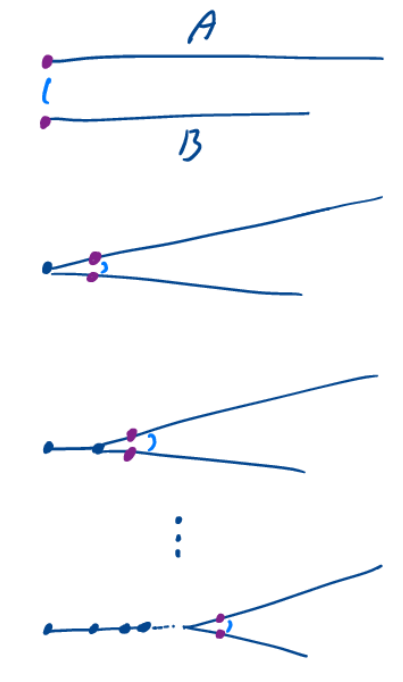
\includegraphics[width = 2.80cm]{immagini/ordine_totale_buoni_ordini.png}
\end{wrapfigure}

\textcolor{MidnightBlue}{\underline{Idea}: Il corollario ci dice che vale al più una delle alternative, quindi la difficoltà risiede nel dimostrare che una si verifica. Molto vagamente potremmo ragionare così.
Identifichiamo, progressivamente, segmenti iniziali sempre più lunghi di $A$ e $B$. All'inizio identifichiamo il minimo di $A$ con il minimo di $B$, poi il secondo elemento di $A$ con il secondo elemento di $B$, etc. Fatti $\omega$
passaggi avremo identificato un segmento iniziale di $A$, diciamo $A_x$, isomorfo a $\omega$, con un $B_y$, anch'esso ovviamente isomorfo a $\omega$. Bene: continuiamo identificando $x$ con $y$. Quando potrebbe bloccarsi il procedimento?
Solo se, ad un certo punto, abbiamo identificato interamente uno dei due insiemi, con un segmento iniziale dell'altro - perché altrimenti, abbiamo identificato due segmenti iniziali $A_x$ e $B_y$ e possiamo continuare attaccando $x$ a $y$. È 
come la chiusura di una cerniera lampo : ad ogni istante c'è un prossimo dente.\\
\textcolor{red}{Questa discorso, però, non è una dimostrazione.} Se vogliamo, sarebbe un tentativo di costruire l'isomorfismo cercato per \textcolor{purple}{ricorsione transfinita}. Il guaio è che i numeri che permetterebbero di numerare i passaggi della costruzione,
gli \textcolor{purple}{ordinali}, sono appunto l'oggetto che stiamo tentando di costruire.}

\begin{proof}
	Per il corollario visto prima, si può verificare al più una delle tre condizioni, altrimenti avremmo un assurdo, verifichiamo dunque che se ne verifichi almeno una. Consideriamo $f$ definita come segue:
	\[ f = \{(a,b) \in A \times B | A_a \sim B_b\}
		\]
	Vogliamo dimostrare che $f$ è una funzione crescente, che $\Dom(f)$ è un segmento iniziale di $A$, e che $\Imm(f)$ è un segmento iniziale di $B$, da cui $f$ manda segmenti iniziali in segmenti iniziali. Quindi $f$ è un isomorfismo fra un segmento iniziale di $A$ e uno di $B$.
	Infine dimostriamo che necessariamente $\Dom(f) = A$ o $\Imm(f) = B$, e questo conclude la dimostrazione perché se si verifica una delle due o tutte e due, abbiamo ottenuto la tesi del teorema. Procediamo ora con tutte le verifiche.
	\begin{itemize}
		\item[$\boxed{\text{$f$ è una funzione}}$] \textcolor{MidnightBlue}{Supponiamo per assurdo $(a,b) \in f$ e $(a,b') \in f$ con $b \ne b'$. Senza perdita di generalità supponiamo $b < b'$ (quindi $B_b$ s.i. proprio di $B_{b'}$), e, per la definizione data di $f$ ciò corrisponde a:
		\[ B_b \sim A_a \sim B_{b'}
			\]
		dunque $B_{b'}$ sarebbe isomorfo al suo segmento iniziale proprio $B_b$ $\lightning$.}
		\item[$\boxed{\text{$f$ è crescente}}$] \textcolor{MidnightBlue}{Dati $a,a' \in A$, con $a<a'$, dobbiamo dimostrare $f(a) < f(a')$. Supponiamo, per assurdo $f(a') \leq f(a)$, abbiamo allora:
		\[ A_{a'} \sim B_{f(a')} \preceq B_{f(a)} \sim A_a
			\]
		dove i due isomorfismi, vengono semplicemente dalla definizione di $f$, e $B_{f(a')} \preceq B_{f(a)}$ segue da $B_{f(a')} \subseteq B_{f(a)}$, che vale perché stiamo supponendo $f(a') \leq f(a)$ per ipotesi assurda.
		Abbiamo quindi ottenuto che $A_{a'}\preceq A_a$, ovvero $A_{a'}\subseteq A_a \implies a' \leq a$, che è assurdo perché avevamo per ipotesi $a < a'$.}
		\item[$\boxed{\text{$\Dom(f)$ è s.i. di $A$}}$] \textcolor{MidnightBlue}{Sia $a \in \Dom(f)$ e $a' < a$, vogliamo dimostrare che $a' \in \Dom(f)$. L'ipotesi $a \in \Dom(f)$ equivale a dire che $A_a \sim B_b$, per qualche $b \in B$,
		inoltre, essendo $a' < a$ si ha $A_{a'} \subsetneq A_a \to A_{a'} \prec A_a$, per cui $A_{a'} \prec B_b$. A questo punto esiste $b' \in B_b \subsetneq B$ tale che $A_{a'} \sim (B_{b})_{b'}$, per definizione di $\prec$, e, osservando che $(B_b)_{b'} = B_{b'}$,
		si ha proprio $A_{a'} \sim B_{b'} \implies (a',b') \in f$, per cui $a' \in \Dom(f)$.}
		\item[$\boxed{\text{$\Imm(f)$ è s.i. di $B$}}$] \textcolor{MidnightBlue}{Dimostrazione simmetrica alla precedente.}
		\item[$\boxed{\begin{aligned}\text{$\Dom(f) = A$} \\ \text{o $\Imm(f) = B$}\end{aligned}}$] \textcolor{MidnightBlue}{Se così non fosse, per la terza e quarta verifica, avremmo contemporaneamente $\Dom(f) = A_a$ e $\Imm(f) = B_b$ \footnote{Stiamo negando un OR quindi l'unica possibilità è che siano entrambe false.},
		per opportuni $a \in A$ e $b \in B$. Per la seconda verifica $f$ è crescente, quindi è un isomorfismo fra $\Dom(f) = A_a$ e $\Imm(f) = B_b$, pertanto,
		si ottiene proprio $A_a \sim B_b$, e quindi, per definizione di $f$, $(a,b) \in f$, da cui $a \in \Dom(f) = A_a \; \lightning$ (oppure $b \in \Imm(f) = B_b \; \lightning$). Segue quindi che almeno una delle due condizioni è sempre vera.}
	\end{itemize}
\end{proof}

\begin{exercise}[Sottoinsiemi propri e buoni ordinamenti]
	Sia $(A,<)$ un buon ordine e sia $B \subsetneq A$. Dimostra che $B \preceq A$, ma non necessariamente $B \prec A$.
\end{exercise}

\begin{soln}
	In primis osserviamo che non può valere $A \prec B$, infatti, se $A$ fosse isomorfo ad un segmento iniziale proprio di $B$, sia $B_b$, per $b \in B$,
	allora $b \leq f(b)\footnote{Notare che la disuguaglianza continua a valere solo perché $B \subseteq A$, in generale se i buoni ordinamenti sono diversi non vale.} \in B_b \implies b \leq f(b) < b \; \lightning$. Per il teorema appena dimostrato sappiamo che la classe dei buoni ordini è totalmente ordinata, per cui vale necessariamente $B \preceq A$.\\
	Per avere un controesempio di $B \subsetneq A \notimplies B \prec A$ ci basta considerare $(\omega,<)$ e il sottoinsieme proprio $2\omega$ dei numeri pari, in questo caso infatti abbiamo $(2\omega,<_{|2\omega}) \sim (\omega,<)$,
	che è dato dalla funzione che mappa $i \mapsto n_i$ (l'$i$-esimo numero pari preso in ordine strettamente crescente).
\end{soln}

\begin{exercise}[Unione di buoni ordinamenti]
	Sia $(A,<_A)$ un ordine totale con $A = \bigcup S$. Supponiamo che:
	\begin{enumerate}[1.]
		\item ogni $X \in S$ è un buon ordine con la restrizione $<_{A|X}$
		\item per ogni $X,Y \in S$, o $X$ è segmento iniziale di $Y$ o $Y$ è segmento iniziale di $X$
	\end{enumerate}
	Dimostra che allora $(A,<_A)$ è un buon ordine. Esibisci inoltre un controesempio alla tesi eliminando la condizione 2 dalle ipotesi.
\end{exercise}

\begin{soln}
	Dato $B \subseteq A$ diverso dal vuoto, allora, detto $Z = \{X \in S | X \cap B \ne \emptyset\}$, possiamo considerare $\bigcap Z$ ed osservare che $\bigcap Z = X \in Z$, infatti,
	se per assurdo ci fosse almeno un elemento di un altro insieme, $y \in \bigcap Z$, con $y \in Y \in S \land y \not \in X$, allora, essendo che per ipotesi o $X$ è segmento iniziale di $Y$ o viceversa, si ha: nel primo caso $y$ non può stare nell'intersezione perché non appartiene ad $X$, per cui abbiamo un assurdo,
	nel secondo - se $Y$ segmento iniziale di $X$ - avremmo che $y \in X$ e quindi ancora un assurdo.\\
	Abbiamo quindi che $\emptyset \ne \bigcap Z = X \in Z$, per cui $X \cap B \ne \emptyset$, ed è ben definito $b = \min_{<_{A|X}} (X \cap B) = \min_{<_{A|X}} \left(\bigcap Z \cap B\right)$.\\
	Non resta che osservare che $b$ è il minimo anche per gli elementi di $B \setminus X$. Dato $b' \in B \setminus X$, allora $b' \in Y \in Z$, con $Y \ne X$, osserviamo ora che $X$ è segmento iniziale di $Y$ (deve valere una delle due cose per ipotesi, ed essendo $X = \bigcap Z \subseteq Y$, siamo necessariamente in questo caso),
	per cui $X = Y_c$ (siamo in un buon ordinamento), per qualche $c \in Y$, e in particolare si ha proprio $b < c \leq b'$, infatti la prima disuguaglianza è banale, mentre la seconda deriva dal fatto che $b' \in B \setminus X$ 
	e per la proprietà dei segmenti iniziali se fosse $b' < c$ allora $b' \in Y_c = X$ che è assurdo.\\
	Per il controesempio alla tesi nel caso in cui manchi la seconda condizione, consideriamo l'insieme $\QQ = \{q_n | n \in \omega\}$ di cui abbiamo fissato un'enumerazione, detto $Q_n = \{q_i | i < n\}$, naturalmente si ha:
	\[ \QQ = \bigcup_{n \in \omega} Q_n
		\]
	dove $(\QQ,<)$ è totalmente ordinato e i $(Q_n,<_{|Q_n})$ sono bene ordinati dalla restrizione dell'ordinamento di $\QQ$ essendo insiemi finiti, inoltre non è vero che presi $Q_n$ e $Q_m$ uno non è necessariamente segmento iniziale dell'altro,
	perché nell'enumerazione possiamo (e necessariamente dovrà accadere) aggiungere anche elementi più piccoli. Siamo pertanto nelle condizioni dell'esercizio tranne che per 2., e quindi naturalmente non si ottiene che $(\QQ,<)$ è bene ordinato.
\end{soln}

\subsection{Operazioni aritmetiche fra buoni ordinamenti}
Per ora, non abbiamo visto molti esempi di buoni ordini. Le operazione definite in questa sezione forniscono una prima sorgente di esempi concreti.
Nel seguito del corso, vedremo buoni ordini assai più versatile di quelli ottenibili con queste operazioni.

\begin{definition}[Somma di ordini totali]
	Dati $(A,<_A)$ e $(B,<_B)$ ordini totali. Definiamo la \vocab{somma di ordini totali} come:
	\[ (A,<_A) + (B,<_B) \Mydef (A \sqcup B, <_+)
		\]
	dove, ricordiamo che $A \sqcup B = (A \times\{0\}) \cup (B \times \{1\})$, e $<_+$ è definito da:
	\[ \begin{split}
		(x,y) <_+ (x',y') &\Mydef (y = 0 \land y' = 1) \\
						  &\lor (y = 0 \land y' = 0 \land x <_A x') \\
						  &\lor (y = 1 \land y' = 1 \land x <_B x')
	\end{split}
		\]
\end{definition}

\textcolor{MidnightBlue}{L'idea è che $(A,<_A) + (B,<_B)$ si ottiene attaccando $(B,<_B)$ in coda a $(A,<_A)$}.

\begin{figure}[H]
	\centering
	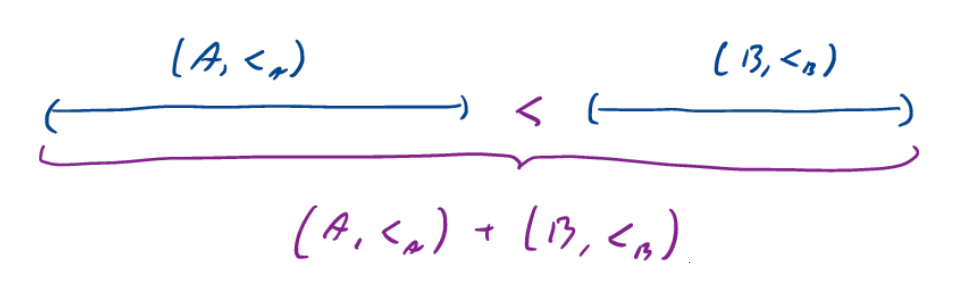
\includegraphics[width = 7.5cm]{immagini/somma_ordini_totali.png}
\end{figure}

Riproponiamo, per completezza, la definizione di prodotto lessicografico.

\begin{definition}[Prodotto di lessicografico]
	Siano $(A,<_A)$ e $(B,<_B)$ ordini totali. Definiamo il \vocab{prodotto del lessicografico}:
	\[ (A,<_A) \cdot (B,<_B) \Mydef (A \times B, <_\times)
		\]
	dove $<_\times$ è definito da:
	\[ (x,y) <_\times (x',y') \Mydef (y <_B y') \lor (y = y' \land x <_A x')
		\]
\end{definition}

\textcolor{MidnightBlue}{L'idea di confrontare prima la seconda componente, deriva dal fatto che $(A,<_A) \cdot (B,<_B)$ sono 
tante copie di $(A,<_A)$ giustapposte, quanti sono gli elementi di $B$ (e quindi associate nello stesso ordine)}.

\begin{figure}[H]
	\centering
	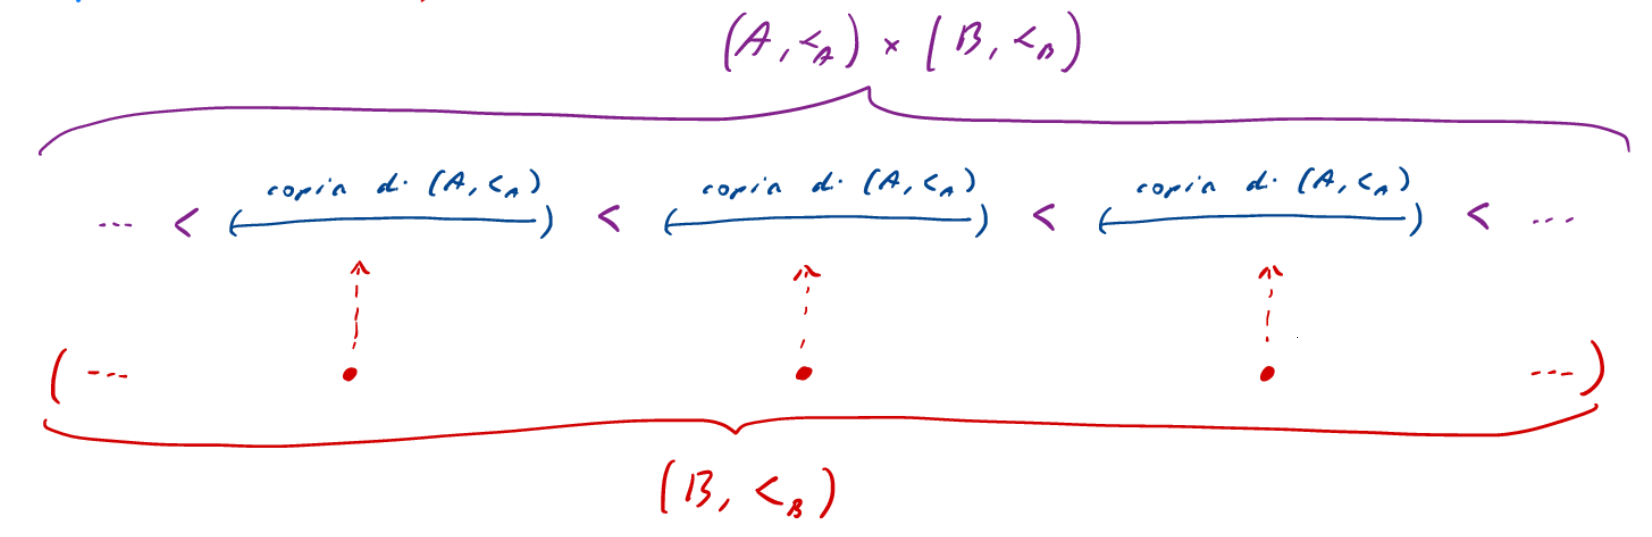
\includegraphics[width = 10.5cm]{immagini/ordine_lessicografico.png}
\end{figure}

Per definire l'esponenziale ci serve la nozione di supporto.

\begin{definition}[Supporto di una funzione da un insieme a un buon ordine]
	Dato un buon ordine $(B,<)$ e $f : A \rightarrow B$, il \vocab{supporto} di $f$ è:
	\[ \supp_B(f) \Mydef \{x \in A | f(x) \ne \min_{<_B} B\}
		\]
	(ometteremo il pedice $B$ quando è chiaro cosa sia $B$).
\end{definition}

\textcolor{MidnightBlue}{Il supporto è quindi il sottoinsieme dei punti sull'insieme di partenza, sui quali $f$ non assume il minimo del buon ordinamento in arrivo quest'ultimo.}

\begin{definition}[Esponenziali di ordini totali]
	Dati $(A,<_A)$ e $(B,<_B)$ ordini totali, definiamo l'\vocab{esponenziale di ordini totali}:
	\[ (A,<_A)^{(B,<_B)} \Mydef (\{f \in {}^{B}A \, : \, |\supp_A f| < \aleph_0\},<_{\exp})
		\]
	dove l'insieme è quello delle funzioni a supporto finito (quindi che su un numero finito di punti non assumono il valore $\min_{<_B}B$), e l'ordine $<_{\exp}$ è definito da:
	\[ f <_{\exp} g \Mydef (f \ne g) \land (f(m) <_A g(m))
		 \]
	dove $m$ è il massimo valore in $B$ su cui $f$ e $g$ sono diverse, cioè non sono entrambe $\min A$, $m := \max_{<_B}\{x \in B | f(x) \ne g(x)\}$.
\end{definition}

\textcolor{MidnightBlue}{L'idea è che una funzione $B \rightarrow A$ può essere vista come una specie di tupla con tante componenti quanti sono gli elementi di $B$\footnote{D'altronde abbiamo visto che $|{}^{B}A| = |A|^{|B|}$, il che ci fa notare che la definizione data di insieme di funzioni come una sorta di esponenziazione di un insieme ad un altro, è coerente con quella di esponenziazione come prodotto cartesiano ripetuto un numero di volte pari alla cardinalità dell'esponente, da qui l'identificazione di ${}^{B}A$ con $\underbrace{A \times \ldots \times A}_{\text{$|B|$ volte}}$, che ci dà l'intuizione descritta (e che formalmente si traduce nell'insieme di funzioni, che sarà poi la vera definizione di prodotto cartesiano).}.
Ordinare queste tuple lessicograficamente significa (generalizzando l'idea usata per il prodotto lessicografico) che vince la componente diversa più a destra, e se definitivamente c'è il minimo in entrambe le tuple, per la finitezza del supporto, basta confrontare l'ultima componente dove sono diverse, ossia la componente corrispondente all'elemento di $B$ più grande su cui le funzioni sono diverse.}

\begin{exercise}
	Verificare che $(\omega,<)^{(\omega,<)} \sim (\NN[x],\prec)$, dove $\NN[x]$ denota l'insieme dei polinomi a coefficienti in $\NN$, e definiamo:
	\[ p \prec q \Mydef \exists N \in \NN \; \forall x \in \NN \; x > N \rightarrow p(x) < q(x)
		\]
	ossia $p \prec q$ se $p(x)<q(x)$ definitivamente.
\end{exercise}

\begin{soln}
	Possiamo scrivere esplicitamente l'isomorfismo come segue:
	\[ (\omega,<)^{(\omega,<)} \to (\NN[x],\prec) : f \mapsto \sum_{i = 0}^{\infty}f(i)x^i
		\]
	osserviamo in primis che la sommatoria è in realtà una somma di un numero finito di termini in quanto $f$ ha supporto finito,
	dunque ciò che otteniamo è un polinomio e quindi la mappa è ben definita. Si vede facilmente che è surgettiva, infatti, dato $p(x) = \sum_{i = 0}^n a_i x^i$, 
	è sufficiente considerare:
	\[ f : \omega \to \omega : i \mapsto \begin{cases}
		a_i &\text{se $0 \leq i \leq n$} \\
		0 &\text{altrimenti}
	\end{cases}
		\] 
	che è naturalmente una funzione a supporto finito dai naturali ai naturali. Infine, verifichiamo la stretta crescenza, date $f < g$, abbiamo $f(m) < g(m)$, 
	per $m$ massimo valore in $\omega$ per cui sono distinte; si danno due casi, o $f(m) = 0$ e quindi $g(m) > 0$, in questo caso a $g$ corrisponde un polinomio $q(x)$ di grado 
	più grande strettamente, dunque, se $f$ corrisponde a $p(x)$, si ha $q(x) = \text o(p(x))$ per $x \to +\infty$, per cui $\lim_{x \to +\infty} \frac{q(x)}{p(x)} = +\infty$, che equivale alla definizione data di $p \prec q$.
	Nel caso in cui $f(m) > 0$, allora $p(x)$ e $q(x)$ sono polinomi dello stesso grado, ma $q(x)$ ha coefficiente di testa maggiore strettamente di quello di $p(x)$,
	per cui $\lim_{x \to +\infty} \frac{q(x)}{p(x)} > 0 \implies p \prec q$.
\end{soln}

\begin{proposition}[Somma, prodotto ed esponenziale di buoni ordini è un buon ordine]
	Se $(A,<_A)$ e $(B,<_B)$ sono buoni ordini, allora anche:
	\[ (A,<_A) + (B,<_B) \qquad (A,<_A) \cdot (B,<_B) \qquad (A,<_A)^{(B,<_B)}
		\]
	sono buoni ordini.
\end{proposition}

\begin{proof}
	Si tratta di banali verifiche, \textcolor{red}{eccetto la terza}.\\
	La relazione $<_{\exp}$ è irriflessiva per definizione richiede $f \ne g$, dunque se sono uguali non sono in relazione. Occorre quindi verificare la transitività.
	Assumiamo $f <_{\exp} g$ e $g <_{\exp} h$, dove naturalmente $f,g,h \in {}^B A$, e poniamo:
	\begin{align*}
		&m_1 = \max_{<_B}\{x\in B | f(x) \ne g(x)\} \\
		&m_2 = \max_{<_B}\{x\in B | g(x) \ne h(x)\} \\
		&m_3 = \max_{<_B}\{x\in B | f(x) \ne h(x)\}
	\end{align*}
	detto $m := \max(m_1,m_2)$, abbiamo $f(m) \leq_A g(m) \leq_A h(m)$, dove la prima disuguaglianza è stretta se $m = m_1$, e la seconda lo è se $m = m_2$, in ogni caso, almeno una delle due disuguaglianze è sempre stretta per cui abbiamo $f(m) <_A h(m)$.
	Osserviamo inoltre che se $x > m$ allora necessariamente $f(x) = g(x) = h(x)$ perché avremmo in questo caso che $x > m_1,m_2$, che sono i massimi su cui si hanno le disuguaglianze, per cui $m = m_3$.\\
	Mostriamo ora che $<_{\exp}$ è un ordine totale, se $f \ne g$ allora è ben definito $m := \max_{<_B}\{x \in B | f(x) \ne g(x)\}$, infatti le funzioni sono a supporto finito per ipotesi dunque stiamo prendendo il massimo su un insieme finito e 
	non vuoto essendo le funzioni diverse, si conclude per la totalità di $<_A$ che vale necessariamente o $f(m)<_A g(m)$ o $g(m) <_A f(m)$, nel primo caso $f <_{\exp} g$, nel secondo $g <_{\exp} f$.\\
	Resta da verificare che l'ordine ottenuto esponenziando è buono. Chiamiamo $S$ l'insieme delle funzioni a supporto finito da $B$ ad $A$ e supponiamo per assurdo che non sia bene ordinato, cioè:
	\[ \underbrace{\exists f \in S \; \exists A \subseteq S (f \in A}_{\text{c'è un $A \subseteq S$ non vuoto}}\land\underbrace{\forall g \in A \; \exists h \in A \; h <_{\exp} g}_{\text{che non ha minimo}})
		\]
	Da quanto appena scritto possiamo fissare una $f \in S$ tale che $\exists A \subseteq S$ etc. con queste proprietà:
	che il massimo del suo supporto sia il minimo possibile, $m:=\max_{<_B}(\supp_A(f))$, e che, a parità di $m$, il valore di $f(m)$ sia minimo.
	Fissata $f$ come scritto, possiamo fissare ora anche $A$ nella formula in modo tale che $f \in A$ ed $A$ sia un sottoinsieme senza minimo.
	Il nostro obiettivo ora è costruire $\widetilde{A} \subseteq S$ che non abbia minimo e contenga una funzione $\widetilde{f}$ con $\widetilde{m} := \max_{<_B}(\supp_A(f)) <_B m$, in questo modo neghiamo la minimalità di $m$ ed otteniamo la contraddizione voluta.
	Osserviamo innanzitutto che $A$ può essere ripartito in generale come:
	\begin{align*}
		&A_1 = \{g \in A |\max_{<_B}(\supp_A(g)) <_B m\} \\
		&A_2 = \{g \in A |\max_{<_B}(\supp_A(g)) = m \land g(m) = f(m)\} \\
		&A_3 = \{g \in A |\max_{<_B}(\supp_A(g)) = m \land f(m) <_A g(m)\} \\
		&A_4 = \{g \in A |m <_B \max_{<_B}(\supp_A(g))\}
	\end{align*}
	e segue dalla definizione che le funzioni in $A_1$, sono $<_{\exp}$ di quelle in $A_2$, che sono $<_{\exp}$ etc. fino ad $A_4$ - è sufficiente pensare alle definizioni che abbiamo dato -.
	Però $A_1$ è vuoto, perché altrimenti, presa $f' \in A_1$, abbiamo $f' \in A$ e $\max(\supp_A(f))<m$ contro la minimalità di $m$.
	Abbiamo invece che $A_2$ non è vuoto perché contiene $f$, e non ha minimo, infatti, se avesse minimo, questo dovrebbe essere anche minimo di $A$ - per la minimalità di $m$, avremmo preso la $f$ che fa meno su $m$ e quindi necessariamente la più piccola di tutte -, che non ha minimo per ipotesi.\\
	Concentriamoci ora su $A_2$. Tutte le $g \in A_2$ assumono il medesimo valore su $m$, quindi, comparando due di queste funzioni con $<_{\exp}$, il valore assunto da entrambe su $m$ 
	è irrilevante perché $<_{\exp}$ confronta la massima componente in cui sono diverse, per cui la funzione:
	\[ H : A_2 \rightarrow S : g \mapsto \widehat{g} \quad\text{con}\quad\widehat{g}(x) = \begin{cases}
		\min A &\text{se $x = m$}\\
		g(x) &\text{altrimenti}
	\end{cases}
		\]
	è strettamente crescente, poiché dove le funzioni sono uguali poniamo semplicemente il loro valore uguale a $\min A$, cosa ininfluente per $<_{\exp}$, mentre dove vale la disuguaglianza continua a valere nell'immagine poiché 
	non modifichiamo nulla in tal caso. Per cui $\widetilde{A} := H[A_2]$ non ha minimo, altrimenti, essendo $H$ strettamente crescente, tornando indietro anche $A$ lo avrebbe.
	Ora, però, segue dalla definizione di $H$, che, fissata $g \in A_2$, $\supp(\widehat{g}) = \supp(g) \setminus \{m\}$ (lo abbiamo rimosso ``a mano'' con $H$), quindi, ponendo $\widetilde{f} := \widehat{g}$, abbiamo $\max(\supp(\widehat{f}))<m$ (prima $m$ era il massimo valore del supporto e non dava $\min A$, ora 
	che l'abbiamo rimosso dal supporto, avendolo preso come il max del precedente supporto, ciò che rimane è necessariamente strettamente minore), e questo contraddice la minimalità di $m$.\footnote{Cose che andrebbero verificate per rendere precisa questa dimostrazione: perché posso fissare $A$ e $f$ tali che..., in altre parole perché esistono $A$ ed $f$ tali per cui...; perché 
	si può partizionare $A$ in quei 4 insiemi; fare le verifiche delle disuguaglianze tra gli elementi dei 4 insiemi; precisare meglio i dettagli della parte finale.}
\end{proof}

\begin{proposition}[Buona definizione delle operazioni tra ``classi di isomorfismo'']
	Le operazioni aritmetiche sui buoni ordini \vocab{passano al quoziente modulo isomorfismi}. Ossia, dati due buoni ordinamenti $\mathcal A = (B,<_A)$
	e $\mathcal B = (B,<_B)$, e dati $\mathcal A' = (A',<_{A'}) \sim \mathcal A$ e $\mathcal{B}' = (B',<_{B'}) \sim \mathcal B$, si ha:
	\[ \mathcal{A} + \mathcal{B} \sim \mathcal{A}' + \mathcal{B'} \qquad \mathcal{A} \cdot \mathcal{B} \sim \mathcal{A}' \cdot \mathcal{B'} \qquad \mathcal{A}^{\mathcal{B}} \sim \mathcal{A}'^{\mathcal{B'}}
		\]
	quindi le operazioni fra buoni ordini sono equivalenti modulo l'essere isomorfi.\footnote{In altre parole le operazioni tra buoni ordini sono definite sulle classi di equivalenza di buoni ordini isomorfi, e la proposizione mostra che queste 
	operazioni sono ben definite.}
\end{proposition}

\begin{proof}
	Fissati gli isomorfismi $f : A \rightarrow A'$ e $g : B \rightarrow B'$, è facile scrivere esplicitamente gli isomorfismi richiesti. Per esempio, nel caso di $\mathcal{A}^{\mathcal{B}}$, si considera la restrizione alle funzioni a supporto finito di:
	\[ {}^{B}A \rightarrow {}^{B'}A' : h \mapsto f \circ h \circ g^{-1}
		\]
	in altre parole, l'isomorfismo richiesto per dimostrare la tesi, che è quello scritto sopra, è quello che manda $h$ nella mappa che fa commutare il seguente diagramma:
	\[\begin{tikzcd}
		B & A \\
		{B'} & {A'}
		\arrow["h", from=1-1, to=1-2]
		\arrow["{g^{-1}}", from=2-1, to=1-1]
		\arrow[from=2-1, to=2-2]
		\arrow["f", from=1-2, to=2-2]
	\end{tikzcd}\]
	andrebbe verificato che anche la nuova funzione $f \circ h \circ g^{-1}$ sia a supporto finito, ma questo segue dal fatto che $f$ e $g$ sono isomorfismi di ordini,
	in particolare vale che $g^{-1}[\supp_{A'}(f \circ h \circ g^{-1})] = \supp_A(h)$ (va verificato il doppio contenimento e può essere fatto facilmente tenendo conto e seguendo il diagramma sopra),
	da cui la bigezione e quindi la finitezza di $\supp_{A'}(f \circ h \circ g^{-1})$.
\end{proof}

\begin{exercise}[Buona definizione delle operazioni tra buoni ordini]
	Fare le altre verifiche della proposizione sopra.
\end{exercise}

\begin{proposition}[Proprietà delle operazioni sui buoni ordini]
	Siano $\mathcal{A} = (A,<_A)$, $\mathcal{B} = (B,<_B)$ e $\mathcal{C} = (C,<_C)$ buoni ordini. Allora:\footnote{Valgono in realtà anche l'esistenza e le proprietà degli elementi neutri per $\cdot$ e $+$.}
	\[\begin{split}
		\text{\textcolor{red}{associatività:}} &\quad (\mathcal A + \mathcal B) + \mathcal C \sim \mathcal A + (\mathcal B + \mathcal C) \quad (\mathcal A \cdot \mathcal B) \cdot \mathcal C \sim \mathcal A \cdot (\mathcal B \cdot \mathcal C)\\
		\text{\textcolor{red}{distributività a sinistra:}} &\quad  \mathcal A \cdot (\mathcal B + \mathcal C) \sim \mathcal A \cdot \mathcal B + \mathcal A \cdot \mathcal C \\
		\text{\textcolor{red}{proprietà delle potenze:}} &\quad {\mathcal A}^{\mathcal B + \mathcal C} \sim \mathcal A^{\mathcal B} \cdot {\mathcal A}^{\mathcal C} \qquad ({\mathcal A}^{\mathcal B})^{\mathcal{C}} \sim {\mathcal A}^{\mathcal B \cdot \mathcal C}
	\end{split}\]
\end{proposition}

\begin{proof}
	Facili verifiche.
\end{proof}

\begin{exercise}[Proprietà delle operazioni tra buoni ordini]
	Fare qualcuna delle verifiche delle proprietà sopra.
\end{exercise}

\textcolor{red}{Non} tutte le proprietà delle operazioni aritmetiche su $\omega$ valgono per i buoni ordini.

\begin{exercise}[Proprietà \textcolor{red}{false} delle operazioni tra buoni ordini]
	Esibire controesempi alle seguenti:
	\textcolor{red}{\begin{align*}
		& \mathcal A + \mathcal B \sim \mathcal B + \mathcal A &(\mathcal A + \mathcal B) \cdot \mathcal C \sim \mathcal A \cdot \mathcal C + \mathcal B \cdot \mathcal C \\
		& \mathcal A \cdot \mathcal B \sim \mathcal B \cdot \mathcal A &(\mathcal A \cdot \mathcal B)^{\mathcal C} \sim \mathcal A^{\mathcal C} \cdot \mathcal B^{\mathcal C}
	\end{align*}}
	ovvero non valgono: \textcolor{red}{commutatività}, \textcolor{red}{distributività a destra} e \textcolor{red}{potenza di un prodotto}.
\end{exercise}

\begin{soln}
	Vediamo controesempi caso per caso.
	\begin{itemize}
		\item[\textcolor{red}{$\boxed{\text{commutatività $+$}}$}] Basta considerare $1+\omega$ e $\omega + 1$ (sia $1$ che $\omega$ sono buoni ordini), infatti abbiamo che:
		\begin{align*}
			1+\omega = (1 \sqcup \omega, <_+) \qquad \omega + 1 = (\omega \sqcup 1, <_+) 
		\end{align*}
		dove $1 \sqcup \omega = (1,0)\cup (\omega \times \{1\}) = \{(1,0),(0,1),(1,1),(2,1),\ldots\}$, con $<_+$ che è l'ordine dato dalla somma di buoni ordini, dunque $(1,0)<_+(n,1)$, $\forall n \in \omega$. Si vede facilmente
		quindi che $1 + \omega$ (oltre ad essere un buon ordine in quanto somma di buoni ordini) è superiormente illimitato e vale il principio del massimo, dunque $1+\omega \sim \omega$. Viceversa, dove $\omega \sqcup 1 = (\omega \times \{0\})\cup \{(1,1)\} = \{(1,1),(0,0),(1,0),(2,0),\ldots\}$,
		con $<_+$ che è sempre l'ordine dato dalla somma di buoni ordini, ma in questo caso si ha $(n,0) <_+ (1,1)$, $\forall n \in \omega$, dunque $\omega + 1$ è superiormente limitato, pertanto non può essere isomorfo ad $\omega$, dunque $1 + \omega \ne \omega + 1$.
		\item[\textcolor{red}{$\boxed{\text{commutatività $\cdot$}}$}] È sufficiente considerare $2 \cdot \omega$ e $\omega \cdot 2$, infatti in questo caso i buoni ordinamenti sono:
		\[ (2 \times \omega,<_\times) \qquad (\omega \times 2, <_\times)
			\]
		Si osserva che $(2 \times \omega,<_\times) \sim (\omega,<)$, infatti, detto $n_i$ l'$i$-esimo numero pari e $m_i = n_i+1$ l'$i$-esimo numero dispari, la mappa $(0,i) \mapsto n_i$ e $(1,i) \mapsto m_i$ è l'isomorfismo cercato. D'altra parte, per le proprietà sopra, si ha $\omega \cdot 2 = \omega \cdot (1 + 1) = \omega + \omega$,
		e non si può avere isomorfismo in quanto $\omega$ è naturalmente isomorfo al segmento iniziale proprio $(\omega,<) \prec \omega + \omega = (\omega \sqcup \omega, <_+)$.
	\end{itemize}
\end{soln}

Un altro tranello in cui si potrebbe cadere è credere che le operazioni sui buoni ordini generalizzino quelle sulle cardinalità. Questo è vero per le cardinalità finite, dove le operazioni di $\omega$ coincidono con quelle cardinali e ordinali, e anche in generale 
per somma e prodotto - come è ovvio dalla definizione - ma fallisce per l'esponenziazione quando consideriamo buoni ordinamenti infiniti.

\begin{exercise}[Cardinalità dell'esponenziazione ordinale]
	Dimostra che se $\mathcal A = (A,<_A)$ e $\mathcal B = (B,<_B)$ sono buoni ordini con $|A| = |B| = \aleph_0$ e $(C,<_C) = \mathcal A^{\mathcal B}$ allora $|C| = \aleph_0$.\footnote{\underline{\textbf{Hint}}: ricordare che $\psf(\omega) = \aleph_0$ e pensare a come si possa identificare ciò con $\omega^\omega$.}
\end{exercise}

\begin{soln}
	A meno di bigezioni, vogliamo dimostrare che $|\omega^\omega| = \aleph_0$, per fare ciò osserviamo che data $f \in \omega^\omega$, essa è a supporto finito, quindi come insieme la si può identificare univocamente come un insieme finito - cioè lasciando solo le coppie corrispondenti 
	a elementi che non danno $\min \omega = 0$ tramite $f$ - per cui si ha che $\{f \in \omega^\omega : |\supp_\omega(f)| < \aleph_0\} \hookrightarrow \psf(\omega \times \omega) : f \mapsto f_{|\supp_\omega(f)}$ è ben definita, e iniettiva (per tornare indietro basta estendere il dominio a tutto $\omega$ ed associare ai nuovi elementi 0).
	Abbiamo quindi $|\omega^\omega| \leq \aleph_0$. Viceversa è ovvio che $\omega \hookrightarrow \omega^\omega : n \mapsto f_n$, ovvero la funzione tale che $f_n(n) = 1$ e $f_n(m) = 0$, per ogni $m \in \omega\setminus\{n\}$, che è ovviamente a supporto finito, per cui abbiamo facilmente l'iniettività e quindi la disuguaglianza dal basso.
\end{soln}

\newpage

\subsection{Gli ordinali di Von Neumann}
In questa sezione definiremo gli ordinali di Von Neumann. L'idea che vogliamo concretizzare è che, siccome abbiamo visto che, 
a meno di isomorfismi, due buoni ordinamenti sono sempre l'uno nell'altro, unendo fra loro tutti i buoni ordinamenti - o tutte le classe di isomorfismo 
di questi - dovrebbe potersi costruire un buon ordinamento più grande di tutti. Questa vasta struttura sarà inevitabilmente una classe propria:
la classe dei \vocab{numeri ordinali}, i cui elementi sono rappresentanti di tutte le possibili classi di isomorfismo di buoni ordini.

\begin{definition}[Insieme transitivo]
	L'insieme $\alpha$ è \vocab{transitivo} se $\forall x \in \alpha \; x \subseteq \alpha$, o equivalentemente, se $\forall x \in \alpha \, \forall y \in x \; y \in \alpha$ (da cui il termine transitivo).
\end{definition}

\textcolor{MidnightBlue}{Ossia: diciamo che $\alpha$ è transitivo se gli elementi degli elementi di $\alpha$ sono, a loro volta, elementi di $\alpha$, cioè se gli elementi sono a loro volta sottoinsiemi dell'insieme insieme (si pensi ad esempio a $\omega$).}

\begin{definition}[Ordinali di Von Neumann]
	L'insieme $\alpha$ è un \vocab{ordinale} se è \textcolor{red}{transitivo e bene ordinato dalla relazione di appartenenza}. Formalmente, l'insieme transitivo $\alpha$
	è un ordinale se $(\alpha, <_\alpha)$ è un buon ordine, con:
	\[ <_\alpha \Mydef \{(x,y) \in \alpha \times \alpha | x \in y\}\,\footnote{Esattamente come accade su $\omega$: $x < y \leftrightarrow x \in y \leftrightarrow (x,y) \in <$.}
		\]
	Denotiamo con \vocab{$\Ord$} la classe degli ordinali\footnote{Tale classe contiene un elemento per ciascun buon ordinamento, ad esempio, preso $(\omega,<)$, come rappresentante della sua classe
	di isomorfismo, prendiamo $\omega$ stesso - inteso come buon ordinamento transitivo e ordinato dall'appartenenza - come rappresentante della ``classe di equivalenza'' nella classe dei buoni ordini (attenzione a non confondere i due significati del termine classe).}, per cui:
	\[ \alpha \in \Ord \Mydef \; \text{``$\alpha$ è transitivo e ben ordinato da $\in$''}
		\]
\end{definition}

\begin{example}[Esempi di ordinali]
	Alcuni esempi di ordinali già incontrati:
	\begin{itemize}
		\item $\omega$ è un ordinale
		\item gli elementi di $\omega$ sono ordinali
		\item $s(\omega) = \omega \cup \{\omega\}$ è un ordinale
	\end{itemize}
\end{example}

\begin{remark}[$\Ord$ è una classe transitiva]
	\label{Ord_trans}
	Se $\alpha \in \Ord$ e $\beta \in \alpha$, allora $\beta \in \Ord$ e $\beta = \alpha_\beta$, ovvero $\beta$ è un ordinale ed è il segmento iniziale principale di $\alpha$, determinato da $\beta$.
	In particolare la classe degli ordinali $\Ord$ è transitiva.\footnote{Cioè tutti gli ordinali sono a loro volta insiemi di ordinali di più piccoli.}
\end{remark}

\begin{proof}
	Siccome $\beta \in \alpha$, per la transitività di $\alpha$, $\beta \subseteq \alpha$, quindi $\beta$ è un sottoinsieme bene ordinato dalla restrizione di $<_\alpha$, ovvero sempre l'appartenenza $\in$.
	La transitività di $\beta$ segue dalla transitività della relazione di ordine $<_{\alpha}$. Prendiamo, infatti, $\delta \in \gamma \in \beta$, vogliamo verificare che $\delta \in \beta$, per fare ciò osserviamo che per la transitività di $\alpha$ si ha:
	\[ \gamma \in \beta \in \alpha \implies \gamma \in \alpha \qquad \delta \in \gamma \in \alpha \implies \delta \in \alpha
		\]
	ora abbiamo quindi $\delta,\gamma,\beta \in \alpha$ e sappiamo che $\delta <_\alpha \gamma \land \gamma <_\alpha \beta$, per cui, essendo $<_\alpha$ transitivo, si ottiene $\delta <_\alpha \beta \equiv \delta \in \beta$, per cui $\beta$ è transitivo.
	Resta da dire che $\beta = \alpha_\beta$:
	\[ x \in \alpha_\beta \overset{\text{def. s.i.}}{\iff} x \in \alpha \land x <_\alpha \beta \overset{\text{def. $<_\alpha$}}{\iff} x \in \alpha \land x \in \beta
		\]
	Ora, essendo che per transitività vale $x \in \beta \rightarrow x \in \alpha$, possiamo quindi eliminare dall'AND il primo termine e ottenere:
	\[ x \in \alpha \land x \in \beta \iff x \in \beta
		\]
	ovvero $x \in \alpha_\beta \leftrightarrow x \in \beta$, dunque per estensionalità $\alpha_\beta = \beta$.
\end{proof}

La proposizione che stiamo per vedere ci dice che due ordinali non possono essere nella stessa classe di isomorfismo di buoni ordini, cioè \textcolor{purple}{per ogni classe di isomorfismo di buoni ordinamenti c'è \textbf{al più} un ordinale}.
Vorremmo poi dimostrare che ogni classe di isomorfismo contiene almeno un ordinale, in modo da poter dire che in ogni classe ce n'è esattamente uno. Vediamo prima della proposizione una semplice osservazione.

\begin{remark}[Gli isomorfismi tra ordini totali mantengono i s.i. principali]
	Se $f : A \rightarrow B$ è un isomorfismo fra $(A,<_A)$ e $(B,<_B)$, allora preso un qualunque $a \in A$ abbiamo $f[A_a] = B_{f(a)}$.
\end{remark}

\begin{proof}
	Basta semplicemente osservare che:
	\[\begin{split}
		x \in B_{f(a)} &\iff x <_B f(a) \\
					   &\iff f^{-1}(x) <_A a \\
					   &\iff f^{-1}(x) \in A_a \\
					   &\iff x \in f[A_a]
	\end{split}
		\]
	e si conclude per estensionalità.
\end{proof}

\begin{proposition}[Gli ordinali isomorfi sono proprio uguali]
	Dati $\alpha,\beta \in \Ord$, se $(\alpha,<_\alpha) \sim (\beta,<_\beta)$, cioè \textcolor{orange}{$\alpha \sim \beta$}, allora \textcolor{orange}{$\alpha = \beta$}.\footnote{La proposizione ha come conseguenza che per ogni classe di isomorfismo di buoni ordinamenti, c'è \textbf{al più} un ordinale, perché se ce ne fosse più di uno - posto che per ora non sappiamo nemmeno se ce ne sia uno - sarebbero esattamente uguali.}
\end{proposition}

\begin{proof}
	Sia $f : \alpha \rightarrow \beta$ un isomorfismo, ci basta dimostrare che $\forall \gamma \in \alpha \; f(\gamma) = \gamma$, cioè che $f = \id_\alpha$. Sia, per assurdo,
	$\gamma$ il minimo elemento di $\alpha$ tale che $f(\gamma) \ne \gamma$, allora:
	\[ \gamma \overset{\text{\hyperref[Ord_trans]{Oss.}}}{=} \alpha_\gamma \overset{(\star)}{=} f[\alpha_\gamma] \overset{\text{Oss. sopra}}{=} \beta_{f(\gamma)} \overset{\text{\hyperref[Ord_trans]{Oss.}}}{=} f(\gamma)\;\textcolor{red}{\lightning}
		\]
	dove $(\star)$ è vero in quanto, abbiamo preso $\gamma$ come il più piccolo ordinale per cui $f$ non è l'identità, e $\alpha_\gamma$ è fatto da cose strettamente più piccole di $\gamma$, dunque $f[\alpha_\gamma] = \alpha_\gamma$.
\end{proof}

Possiamo ora chiederci come si rifletta l'ordinamento totale delle classi di isomorfismo di buoni ordini, dato dalla relazione 
``essere segmento iniziale di'', sugli ordinali. La risposta è che diventa la relazione di appartenenza.

\begin{theorem}[Gli ordinali sono totalmente ordinati dalla ``relazione'' di appartenenza]
	Dati $\alpha,\beta \in\Ord$, vale \textcolor{red}{una e una sola} delle seguenti:\footnote{Essendo gli ordinali una classe propria, come stiamo per vedere, questo teorema ci dice che tale classe è totalmente ordinata.}
	\begin{alignat*}{3}
		\textcolor{purple}{\alpha < \beta =} &\; \alpha \in \beta \;\text{che vale \textcolor{orange}{se e solo se} $(\alpha,<_\alpha) \prec (\beta,<_\beta)$} \\
										     &\; \alpha = \beta \;\text{che vale \textcolor{orange}{se e solo se} $(\alpha,<_\alpha) \sim (\beta,<_\beta)$} \\
		\textcolor{purple}{\alpha < \beta =} &\; \beta \in \alpha \;\text{che vale \textcolor{orange}{se e solo se} $(\beta,<_\beta) \prec (\alpha,<_\alpha)$}
	\end{alignat*}
\end{theorem}

\textcolor{MidnightBlue}{\underline{Notazione}: nella dimostrazione porremo per comodità $\alpha \prec \beta \Mydef (\alpha,<_\alpha) \prec (\beta,<_\beta)$, e analogamente $\alpha \sim \beta$ e $\beta \prec \alpha$.}

\begin{proof}
	La tricotomia vale già sull'ordinamento $\preceq$ per il teorema visto sui buoni ordinamenti, per cui verificando i se e solo se la si ottiene anche su $<$, in tal modo otteniamo che tutti gli ordinali sono totalmente ordinati da $<$. Inoltre,
	nella proposizione precedente abbiamo già verificato che se due ordinali sono isomorfi allora sono proprio uguali - ed il viceversa è triviale -, per cui ora vediamo solo la prima equivalenza essendo la terza perfettamente simmetrica.
	\begin{itemize}
		\item[$\boxed{\Longleftarrow}$] Se $\alpha \prec \beta$, allora per definizione $\alpha$ è isomorfo ad un segmento iniziale proprio - cioè principale -  di $\beta$, $\alpha \sim \beta_\gamma$, per qualche $\gamma \in \beta$, e, per l'\hyperref[Ord_trans]{osservazione} fatta prima, $\beta_\gamma = \gamma$.
		Per cui $\alpha \sim \gamma$ e dalla proposizione precedente otteniamo proprio che $\alpha = \gamma$, quindi si conclude che $\alpha \in \beta$.
		\item[$\boxed{\Longrightarrow}$] Se $\alpha \in \beta$, allora, per l'\hyperref[Ord_trans]{osservazione} solita, sappiamo che $\alpha = \beta_\alpha$, e quindi banalmente, cioè via $\id_\alpha$, si ha $\alpha \prec \beta$.
	\end{itemize}
\end{proof}

\begin{notation}[Ordine della classe degli ordinali]
	Dati $\alpha,\beta \in \Ord$, avendo dimostrato che l'appartenenza è una ``relazione di ordine totale'' per gli ordinali, quando si parla di ordinali useremo la notazione:
	\[ \alpha < \beta \Mydef \alpha \in \beta
		\]
	Infatti il teorema precedente ci dice che la relazione $<$ gode delle proprietà di un ordine totale stretto sulla classe degli ordinali.
\end{notation}

\begin{exercise}[Gli ordinali finiti sono tutti e soli quelli di $\omega$]
	Dimostra che $\alpha$ è un ordinale finito se e solo se $\alpha \in \omega$.
\end{exercise}

\begin{soln}
	Sappiamo già che dato $n \in \omega$, $(n,<_{|n})$ è un buon ordinamento transitivo con l'ordine dato dall'appartenenza, e per definizione è finito, pertanto è banale osservare che tutti gli elementi di $\omega$ sono ordinali finiti.\\
	Viceversa, dato $\alpha$ ordinale finito, poiché è finito è in bigezione con un certo naturale $n \in \omega$, che, come ricordato sopra, è un ordinale a sua volta con l'ordinamento indotto, otteniamo che $n \sim \alpha$. Infatti essendo $n$ ed $\alpha$
	buoni ordinamenti esiste un unico isomorfismo tra loro - ed è dato da $f(i) = \min(\alpha \setminus f[i])$ per $i = 0,\ldots,n-1$, che è surgettivo poiché gli insiemi sono equipotenti e finiti\footnote{Per la precisione stiamo usando il fatto che se $|A| = |B| = n \in \omega$, allora 
	$f : A \to B$ (o viceversa) è iniettiva se e solo se è surgettiva.} -, quindi per la proposizione vista, essendo $\alpha$ ed $n$ ordinali,
	$\alpha \sim n \implies \alpha = n \implies \alpha \in \omega$.
\end{soln}

\begin{proposition}[Ordine largo sulla classe degli ordinali]
	Siano $\alpha,\beta \in \Ord$, allora:
	\[ \alpha \leq \beta \leftrightarrow \alpha \subseteq \beta
		\]
	con $\alpha \leq \beta \Mydef \alpha < \beta \lor \alpha = \beta$.
\end{proposition}

\begin{proof}
	Vediamo le due implicazioni:
	\begin{itemize}
		\item[$\boxed{\longrightarrow}$] Si danno due casi, se $\alpha = \beta$, allora naturalmente ciò vale anche come insiemi per estensionalità. Se $\alpha < \beta$, per definizione $\alpha \in \beta$,
		e poiché $\beta$ è transitivo $\alpha \subseteq \beta$.
		\item[$\boxed{\longleftarrow}$] Dato $\alpha \subseteq \beta$, supponiamo per assurdo che $\beta < \alpha$, allora $\beta \in \alpha \subseteq \beta$, per cui $\beta \in \beta \;\textcolor{red}{\lightning}$,
		infatti $\beta \in \beta \equiv \beta < \beta$, ed avendo dimostrato che $<$ corrisponde a $\prec$, che è un ordine totale, allora naturalmente lo è anche $<$, e quindi in particolare è una relazione d'ordine irriflessiva.\footnote{Segnalo l'osservazione ironica di Mamino nelle dispense originali che fa riferimento a buona fondazione.}
	\end{itemize}
\end{proof}

Ricordiamo che $s(\alpha) \Mydef \alpha \cup \{\alpha\}$. La proposizione seguente ci dice che $s(\alpha)$ è, a buon diritto, il successore di $\alpha$, anche quando $\alpha$
è un ordinale.

\begin{proposition}[Il successore è un ordinale]
	Dato $\alpha \in \Ord$, $s(\alpha)$ è il minimo ordinale $> \alpha$.
\end{proposition}

\begin{proof}
	Occorre inizialmente verificare che $s(\alpha)$ è un ordinale.
	\begin{itemize}
		\item[$\boxed{\text{transitività}}$] Se $\beta \in s(\alpha)$, allora per definizione di successore o $\beta \in \alpha$ o $\beta = \alpha$. Abbiamo naturalmente che $\alpha \subseteq s(\alpha)$,
		dunque nel primo caso la transitività segue da quella di $\alpha$, infatti $\gamma \in \beta = \alpha \implies \gamma \in \alpha \subseteq s(\alpha)$, ovvero $\gamma \in s(\alpha)$.
		Nel secondo caso è proprio banale perché per costruzione appunto $\alpha \subseteq s(\alpha)$.
		\item[$\boxed{\text{buon ordine}}$] Siccome $s(\alpha)$ è un insieme di ordinali, $\in$ è un ordine totale su $s(\alpha)$, per quanto già visto. Dato $X \subseteq s(\alpha) = \alpha \cup \{\alpha\}$, con $X \ne \emptyset$,
		abbiamo due casi, o $X = \alpha$ o $X \cap \alpha \ne \emptyset$. Nel primo caso naturalmente sappiamo che $\alpha$ è bene ordinato e si conclude, nel secondo caso $\min(X) = \min(X \cap \alpha)$,
		infatti il minimo al RHS è ben definito perché $\alpha$ è ben ordinato ed è minimo anche per $X \setminus (X \cap \alpha) = \{\alpha\}$, in quanto appartiene ad $\alpha$.
	\end{itemize}
	Supponiamo ora per assurdo che $s(\alpha)$ non sia il minimo ordinale $> \alpha$, allora esiste $\gamma$ tale che $\alpha < \gamma < s(\alpha)$, dalla prima disuguaglianza segue, per transitività, che $\alpha \subseteq \gamma$,
	inoltre $\alpha \in \gamma \implies {\alpha} \subseteq \alpha$, per cui $s(\alpha) \subseteq \gamma \leftrightarrow s(\alpha) \leq \gamma \; \textcolor{red}{\lightning}$.
\end{proof}

\begin{corollary}[Successore del primo termine in una disuguaglianza tra ordinali]
	$\forall \alpha,\beta \in\Ord \; \beta \leq \alpha \leftrightarrow \beta < s(\alpha)$.
\end{corollary}

\begin{proof}
	Sono due facili verifiche.
	\begin{itemize}
		\item[$\boxed{\longleftarrow}$] Da $\beta < s(\alpha)$, deduciamo per la definizione dell'ordinamento sugli ordinali che $\beta \in s(\alpha) = \alpha \cup \{\alpha\}$,
		che equivale a $\beta \in \alpha$ o $\beta = \alpha$, e, di nuovo per la definizione di ordinamento sugli ordinali, la prima cosa equivale a $\beta < \alpha$, pertanto abbiamo proprio che $\beta \leq \alpha$.
		\item[$\boxed{\longrightarrow}$] Per quanto visto $\beta \leq \alpha \leftrightarrow \beta < \alpha \lor \beta = \alpha$, nel primo caso, per transitività, essendo $\beta < \alpha < s(\alpha)$, si ha $\beta < s(\alpha)$, nel secondo $\beta = \alpha < s(\alpha)$,
		e la seconda disuguaglianza è vera per la proposizione precedente.
	\end{itemize}
\end{proof}

\begin{proposition}[Proprietà degli insiemi di ordinali]
	Dato un insieme di ordinali $X$:
	\begin{enumerate}[1.]
		\item Se $X \ne \emptyset$, allora esiste il minimo di $X$, detto \vocab{$\min X$}, inoltre $\min X = \bigcap X$.\footnote{Da cui si deduce anche che la classe $\Ord$ è bene ordinata usando la stessa idea di questa dimostrazione.}
		\item Esiste il minimo dei maggioranti di $X$ \textcolor{MidnightBlue}{- gli $\alpha \in \Ord$ tali che $\forall \beta \in X \; \beta \leq \alpha$ -}, detto \vocab{$\sup X$}, inoltre $\sup X = \bigcup X$.
		\item C'è almeno un ordinale che non appartiene a $X$.
	\end{enumerate}
\end{proposition}

\begin{proof}
	Vediamo singolarmente i vari punti.
	\begin{enumerate}[1.]
		\item \textcolor{purple}{Dimostriamo che il minimo esiste.} Essendo $X \ne \emptyset$ possiamo fissare $\alpha \in X$. Consideriamo $\mu := \min_{<_{s(\alpha)}}(X \cap s(\alpha))$.
		Questo esiste perché $X \cap s(\alpha) \ne \emptyset$ in quanto $\alpha$ vi appartiene, ed è ben definito perché $s(\alpha)$ è un ordinale. Osserviamo ora che è minimo anche per $X\setminus s(\alpha)$ \textcolor{MidnightBlue}{- di fatto abbiamo tolto da $X$ tutti gli ordinali $\leq \alpha$-},
		preso $\beta \in X \setminus s(\alpha)$ si ha necessariamente che $\beta \geq s(\alpha)$ (altrimenti $\beta < \alpha \equiv \beta \in s(\alpha)$), e poiché $\mu \in s(\alpha)$, si ha $\mu < s(\alpha) \leq \beta$.\\
		\textcolor{purple}{Ora verifichiamo che il minimo $\mu$ sia uguale a $\bigcap X$.} Per definizione di minimo $\forall \gamma \in X \; \mu \leq \gamma \leftrightarrow \mu \subseteq \gamma$, pertanto $\mu \leq \bigcap X$.
		D'altro canto $\mu \in X$, quindi $\bigcap X \subseteq \mu \leftrightarrow \bigcap X \leq \mu$.
		\item Dimostriamo in primis che $\bigcup X$ è un ordinale.
		\begin{itemize}
			\item[$\boxed{\text{transitività}}$] Dato $\alpha \in \bigcup X$, per definizione, esiste $\beta \in X$ tale che $\alpha \in \beta$. Per transitività di $\beta$ si ha $\gamma \in \alpha \in \beta \to \gamma \in \beta$, da cui $\gamma \in \bigcup X$, che quindi è transitivo.
			\item[$\boxed{\text{buon ordine}}$] Ogni $\alpha \in \bigcup X$ appartiene a qualche ordinale $\beta \in X$, pertanto, per la solita \hyperref[Ord_trans]{osservazione sulla transitività di Ord}, $\alpha$ è un ordinale, quindi $\bigcup X$ è un insieme di ordinali - in particolare $\bigcup X \subseteq \Ord$ ed è un insieme per l'assioma dell'unione - ed
			è bene ordinato per il punto 1. della proposizione.\footnote{Questa cosa poteva anche essere dimostrata alternativamente, senza usare il punto 1. facendo invece leva sull'esercizio visto in precedenza dell'unione di buoni ordinamenti che sono uno segmento iniziale dell'altro.}
		\end{itemize}
		Per ogni $\alpha \in X$ si ha, per definizione di unione, $\alpha \subseteq \bigcup X$, che equivale, per quanto visto, a dire $\alpha \leq \bigcup X$, pertanto $\bigcup X$ è un maggiorante di $X$. Osserviamo ora che è il più piccolo maggiorante, infatti, dato $\sigma$ maggiorante di $X$,
		per definizione, $\forall \alpha \in X \; \alpha \leq \sigma \leftrightarrow \alpha \subseteq \sigma$, cioè contiene tutti gli $\alpha \in X$, e quindi in particolare contiene la loro unione, $\bigcup X \subseteq \sigma \leftrightarrow \bigcup X \leq \sigma$.
		\item Basta considerare $s(\sup X)$, per il 2. sappiamo che l'estremo superiore di $X$ esiste, e dalle proprietà viste sugli ordinali, sappiamo che il successore di un ordinale è il minimo ordinale più grande, dunque, in questo caso, $s(\sup X)$ è un maggiorante stretto per $X$, pertanto non sta nell'insieme.
	\end{enumerate}
\end{proof}

\begin{corollary}[Gli insiemi di ordinali transitivi sono ordinali]
	Un insieme di ordinali è un ordinale se e solo se è transitivo.
\end{corollary}

\begin{proof}
	Per il 2. della proposizione precedente sappiamo che ogni insieme di ordinali è ben ordinato - dall'appartenenza naturalmente -, dunque la definizione di ordinale in questo caso si riduce al richiedere la transitività dell'insieme.
\end{proof}

\begin{corollary}[Paradosso di Burali-Forti]
	$\Ord$ è una classe propria.
\end{corollary}

\textcolor{MidnightBlue}{Ossia non esiste l'insieme di tutti gli ordinali.}

\begin{proof}
	Per il punto 3. della proposizione sulle proprietà degli insiemi di ordinali, se $\Ord$ fosse un insieme, esisterebbe un ordinale che non vi appartiene, che è assurdo.
\end{proof}

\begin{note}[Cosa c'è di paradossale nel paradosso di Burali-Forti?]
	Nel 1897, \href{https://it.wikipedia.org/wiki/Cesare_Burali-Forti}{\textcolor{purple}{Cesare Burali-Forti}} era assolutamente convinto della esistenza dell'insieme
	di tutti gli ordinali - definiti allora come le classi di isomorfismo dei buoni ordini - quello che non sapeva è se la relazione $\prec$ fosse un ordine totale su queste classi.
	\begin{figure}[H]
		\centering
		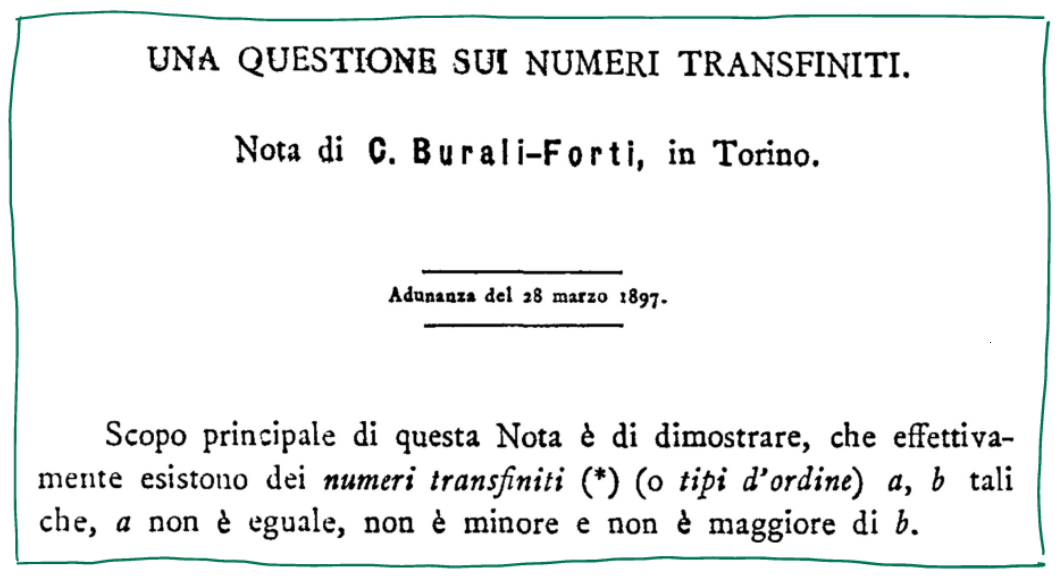
\includegraphics[width = 7.5cm]{immagini/Burali_Forti.png}
	\end{figure}
	Burali-Forti credette di poter negare la totalità dell'ordine $\prec$ ragionando per assurdo. Se $\prec$ fosse un ordine totale, si può dimostrare che è buono esattamente come abbiamo visto sopra, ma 
	allora $\Omega \Mydef [(\Ord,\prec)]$, la classe di isomorfismo di $(\Ord,\prec)$\footnote{Per la precisione stiamo prendendo l'ordinale associato, cosa che non sappiamo ancora fare ma che si può fare come vedremo a breve.},
	sarebbe a sua volta una classe di isomorfismo di un buon ordinamento e quindi uno dei membri della classe $\Ord$ stessa,
	e, considerando il suo successore $s(\Omega)$, avremmo $\Omega \prec s(\Omega)$, ma anche ovviamente $s(\Omega) \prec \Omega$, perché $s(\Omega) \in \Ord\;\textcolor{red}\lightning$.\\
	Il guaio è che, nello stesso anno, Cantor pubblicò una dimostrazione del fatto che la relazione $\prec$ è totale - esattamente l'argomento dei segmenti iniziali isomorfi che abbiamo illustrato 
	nel corso. Come è stata risolta la contraddizione? Concludendo che l'insieme di tutti gli ordinali esiste? \textcolor{red}{No}. Sfortunatamente Burali-Forti 
	aveva capito male la definizione di buon ordinamento, e ancora così, forse, nessuno se ne sarebbe accorto, ma, quel che è peggio, aveva tentato di correggerla, facendo, in realtà un pasticcio.
	La contraddizione è stata quindi imputata, da Burali-Forti e da Cantor, al bisticcio di definizioni ed il paradosso è stato dimenticato. Cinque anni dopo, \href{https://en.wikipedia.org/wiki/Bertrand_Russell}{\textcolor{purple}{Russell}}
	si rese conto del fatto che l'assurdo sussiste anche se si usa la definizione corretta di buon ordinamento, e fu così che il paradosso di Burali-Forti acquisì il suo nome. E tutti vissero felici e contenti.
\end{note}

\subsection{L'assioma del rimpiazzamento}
Gli ordinali di Von Neumann sono eleganti, ma quanti ne abbiamo di questi arnesi? Si può dimostrare che, assumendo i soli assiomi 1-7, il gran totale degli ordinali potrebbe essere:
\[ \textcolor{purple}{\Ord \overset{?}{=} \underbrace{\{\emptyset, s(\emptyset),\ldots,s^n(\emptyset),\ldots,\omega,s(\omega),\ldots,s^n(\omega),\ldots\}}_{\textnormal{\textcolor{MidnightBlue}{in realtà, questo si chiamerà $\omega + \omega$}}}}
	\]
la classe degli ordinali raggiungibili a partire da $\emptyset$ o da $\omega$ con un numero finito di applicazioni della mappa successore.

\begin{exercise}
	Dimostra che la classe descritta sopra è effettivamente una classe, ossia è definita da una formula.
\end{exercise}

\begin{soln}
	Chiamiamo $O = \{\emptyset, s(\emptyset),\ldots,s^n(\emptyset),\ldots,\omega,s(\omega),\ldots,s^n(\omega),\ldots\}$, allora la formula insiemistica che descrive $O$ è:
	\[ x \in O \Mydef (x = \emptyset) \lor (x = \omega) \lor (\exists n \in \omega \; (\underbrace{x = s^n(\emptyset)}_{x = n} \lor \underbrace{x = s^n(\omega)}_{x = \omega + n}))
		\]
	avendo una formula insiemistica ben posta, abbiamo che $O$ è una classe.
\end{soln}

Se vogliamo poter rispondere alla domanda ``quanti ordinali esistono?'' occorre un nuovo assioma: l'assioma del rimpiazzamento. Sotto questa ipotesi addizionale, la risposta sarà
``tutti quelli che potrebbero esistere'', ossia avremo un ordinale per ogni classe di isomorfismo di buoni ordini. Per formulare l'assioma, ci avvarremo dell concetto di funzione classe.

\begin{definition}[Funzione classe]
	Date due classi $A$ e $B$ una \vocab{funzione classe} da $A$ a $B$ è una formula insiemistica $\varphi(x,y)$ tale che:
	\[ \forall x \in A \;\exists \textcolor{red}{!}\,y \in B \; \varphi(x,y)
		\]
\end{definition}

\textcolor{MidnightBlue}{Ossia, una funzione classe è una proprietà, espressa nel linguaggio della teoria degli insiemi, che ad ogni $x \in A$ associa un \textcolor{red}{unico} $y \in B$.}

\begin{notation}[Funzione classe]
	Possiamo denotare una funzione classe $\varphi(x,y)$ da $A$ a $B$ mediante la notazione più familiare:
	\[ F : A \rightarrow B
		\]
	In questo caso, la scrittura $y = F(x)$ è una semplice abbreviazione:
	\[ y = F(x) \Mydef y \in B \land \varphi(x,y)
		\]
\end{notation}

\begin{example}[Esempi di funzioni classe]
	Le seguenti sono funzioni classe $V \rightarrow V$:
	\[ F_1(x) = x \qquad F_2(x) = \{x\} \qquad F_3(x) = \ps(x) \qquad F_4(x) = s(x)
		\]
	La funzione classe $F_5(x) = \sup(x \cap \Ord)$, con $x \cap \Ord \Mydef \{\alpha \in x | \alpha \in \Ord\}$, è $V \rightarrow \Ord$.
\end{example}

\begin{axiom}[Assioma del rimpiazzamento]
	\label{ax8}
	Se $A$ è un \textcolor{LimeGreen}{insieme} e $F : V \rightarrow V$ è una funzione classe, allora $F[A] \Mydef \{F(x) | x \in A\}$ è un \textcolor{LimeGreen}{insieme}.\footnote{Come per la separazione, anche questo è uno \vocab{schema di assiomi}, uno per ogni possibile (formula insiemistica) funzione classe $F$.}
	\[ \forall A \; \exists B \; \forall y \; y \in B \leftrightarrow \exists x \in A \; y = F(x)
		\]
	cioè per ogni insieme esiste un insieme i cui elementi sono immagini di quelli di $A$ per mezzo della funzione classe $F$.
\end{axiom}

\begin{proposition}[Unicità del rimpiazzo]
	Data una funzione classe $F : V \rightarrow V$ vale che:
	\[ \forall A \; \exists\textcolor{red}{!} B \; \forall y \; y \in B \leftrightarrow \exists x \in A \; y = F[x]
		\]
\end{proposition}

\begin{proof}
	Estensionalità.
\end{proof}

\begin{remark}[Rimpiazzamento da insieme a classe]
	Dato un \textcolor{red}{insieme} $A$ e una funzione classe $G : \textcolor{red}{A} \rightarrow V$, esiste ed è unico l'\textcolor{red}{insieme} $G[A]$ tale che:
	\[ \forall y \; y \in G[A] \leftrightarrow \exists x \in A \; y = G(x)
		\]
	in altre parole, l'assioma del rimpiazzamento vale anche con una funzione classe che va da un insieme ad una classe.
\end{remark}

\begin{proof}
	Ci basta semplicemente applicare l'\hyperref[ax8]{assioma del rimpiazzamento} appena enunciato, applicato alla funzione classe $F : V \rightarrow V$ definita come:
	\[ y = F(x) \Mydef (x \in A \land y = G(x)) \lor (x \not \in A \land y = \emptyset)
		\]
	ossia:
	\[ F(x) \Mydef \begin{cases}
		G(x) &\text{se $x \in A$} \\
		\emptyset &\text{altrimenti}
	\end{cases}
		\]
	infatti se $x \in A$ si ha $G(x) = F(x)$, altrimenti c'è il vuoto, per cui $G[A] = F[A]$ è un insieme grazie al rimpiazzamento.
\end{proof}

\begin{exercise}[Esistenza del prodotto cartesiano via rimpiazzamento]
	Dimostra che, dati due insiemi $A$ e $B$, esiste il loro prodotto cartesiano $A \times B$, usando l'assioma del rimpiazzamento ma \textcolor{red}{senza usare l'assioma delle parti}.
\end{exercise}

\begin{soln}
	L'idea è quella di creare l'insieme di tutti gli insiemi del tipo $\{\{a\},\{a,b\}\}$, per tutti gli $a \in A$ e $b \in B$. Per fare questo, fissato $b \in B$ definiamo la funzione classe:
	\[ H : V \to V : x \mapsto \{x,b\}
		\]
	che è ben definita per l'assioma del paio. Ora per rimpiazzamento $H[A] = A_b$ è un insieme \textcolor{MidnightBlue}{- ed è in particolare l'insieme di tutte le coppie $\{a,b\}$ al variare di $a \in A$ -},
	ora possiamo definire la funzione classe:
	\[ G : A_b \to V : \{a,b\} \mapsto \{\{a\},\{a,b\}\}
		\]
	che è ben definita perché di fatto stiamo facendo $\{\{a,b\}\cap A\} \cup \{\{a,b\}\}$, che è ancora un insieme per gli assiomi di singoletto e unione. A questo punto $E_b = G[A_b]$ 
	è un insieme per rimpiazzamento \textcolor{MidnightBlue}{- ed è proprio l'insieme di tutti gli insiemi $\{\{a\},\{a,b\}\}$ per $b$ fissato e $a$ che varia in $A$, cioè è proprio $A \times \{b\}$ -}.
	A questo punto possiamo definire la funzione classe:
	\[ F : B \to V : b \mapsto E_b
		\]
	che è ben definita per quanto osservato e $F[B] = C$ che ci dà l'insieme $\{E_b\}_{b \in B} = \{\{A \times \{b\}\}\}_{b \in B}$ , da cui:
	\[ \bigcup C
		\]
	è l'insieme, per l'assioma dell'unione, di tutte le coppie ordinate $(a,b)$ per $a \in A$ e $b \in B$, ed è quindi proprio $A \times B$.
\end{soln}

\begin{theorem}[Ogni buon ordine è isomorfo ad un unico ordianle]
	Dato un buon ordine $(A,<)$, esiste un unico ordinale $\alpha$ tale che $(A,<)\sim\alpha$.
\end{theorem}

\begin{proof}
	L'unicità segue per quanto abbiamo già visto, cioè $\alpha \sim \alpha' \rightarrow \alpha = \alpha'$. Basta quindi da dimostrare l'esistenza di almeno un ordinale $\alpha$ per ogni classe di isomorfismo di un buon ordinamento. Sia:
	\[ A' = \{x \in A | \exists \gamma \in \Ord \; A_x \sim \gamma\}
		\]
	ovvero l'insieme degli elementi nel buon ordinamento che determinano segmenti iniziali isomorfi ad un qualche ordinale.
	Consideriamo la funzione classe $F : A' \rightarrow \Ord$:
	\[ F(x) = \text{l'unico $\gamma \in \Ord$ tale che $A_x \sim \gamma$}
		\]
	l'unicità segue dalla solita proposizione e ci garantisce che la funzione classe sia ben definita:
	\[ A_x \sim \gamma \land A_x \sim \gamma' \implies \gamma \sim \gamma' \implies \gamma = \gamma'
		\]
	Vogliamo dimostrare che l'insieme $\alpha := F[A'] \sim (A,<)$ - che esiste per rimpiazzamento - è proprio un ordinale isomorfo a $(A,<)$.
	Dimostriamo dunque che $\alpha$ è un ordinale, $A'$ è un segmento iniziale di $A$, $\alpha \sim A'$, e infine che $A' = A$.
	\begin{itemize}
		\item[$\boxed{\text{$\alpha$ è un ordinale}}$] $\alpha$ è definito come l'insieme degli ordinali isomorfi ai segmenti iniziali corrispondenti agli elementi di $A'$, dunque, per un fatto visto, ci basta dimostrare che è transitivo affinché sia un ordinale a sua volta.\\
		Sia $\gamma \in \beta \in \alpha$, con $\beta$ che è per definizione un ordinale isomorfo ad un qualche segmento iniziale principale di $A$, $\beta \sim A_a$, vediamo che anche $\gamma$ è isomorfo ad un segmento iniziale principale di $A$ e quindi $\gamma \in \alpha$.
		Fissato un isomorfismo $f : \beta \to A_a$, possiamo considerarne la restrizione a $\gamma$, che è ancora un isomorfismo, $f_{|\gamma} : \gamma \to (A_a)_{f(\gamma)} = A_{f(\gamma)}$, dove abbiamo usato che gli isomorfismi mandano s.i. in s.i., $f[\gamma] = f[\beta_\gamma] = (A_a)_{f(\gamma)}$, abbiamo quindi ottenuto che $\gamma = F(f(\gamma))$.
		\item[$\boxed{\text{$A'$ s.i. di $A$}}$] Sia $y < x \in A'$, vogliamo verificare che $y \in A'$, poiché $x \in A'$ esiste $\gamma \in \Ord$ tale che $A_x \sim \gamma$, e naturalmente $A_y \subsetneq A_x$. Fissato $f : A_x \to \gamma$ isomorfismo, se verifichiamo che $f[A_y]$ è un ordinale abbiamo concluso poiché si avrebbe $A_y \sim f[A_y] \in \Ord$ e quindi $y \in A'$.
		A questo punto dati $\beta \in \alpha \in f[A_y]$, poiché $A_y$ è un isomorfismo, tornando indietro si ha $f^{-1}(\beta) < f^{-1}(\alpha) \in A_y$, ma poiché $A_y$ è un segmento iniziale, allora $f^{-1}(\beta) \in A_y \iff \beta \in f[A_y]$.\\
		\textcolor{MidnightBlue}{\underline{Alternativa}: Fissato $f : A_x \to \gamma$ isomorfismo, allora $f_{|A_y} : A_y \to \gamma_{f(y)}$ è un isomorfismo perché restrizione di un isomorfismo e sappiamo che gli isomorfismi mandano segmenti iniziali principali in segmenti iniziali principali per un'osservazione vista in precedenza, dunque l'immagine è proprio $\gamma_{f(y)}$, inoltre
		$\gamma_{f(y)} = f(y) \in \Ord$, quindi evitiamo la verifica diretta che l'immagine sia un ordinale.}
		\item[$\boxed{A' \sim \alpha}$] Sia $f : A' \rightarrow \alpha = F[A'] : x \mapsto F(x)$ la funzione tra insiemi, definita per separazione in $A' \times \alpha = A' \times F[A']$ - quindi abbiamo prima ottenuto l'insieme di arrivo con rimpiazzamento e poi ci siamo ristretti a quest'ultimo per avere una funzione -. Dimostriamo che $f$ è un isomorfismo di ordini.\\
		La surgettività è immediata perché, per costruzione, abbiamo che $\alpha = F[A'] \overset{\text{def. $f$}}{=} f[A']$. Osserviamo ora che la stretta crescenza deriva dall'ordinamento dei segmenti iniziali:
		\[ x <_A y \implies f(x) \sim A_x \prec A_y \sim f(y)
			\]
		dove gli isomorfismi sono per definizione di $f$, e la disuguaglianza tra i segmenti iniziali come buoni ordinamenti deriva banalmente da $x < y$. Segue quindi che $f(x) \prec f(y)$, ed essendo ordinali ciò significa proprio che $f(x) \in f(y) \equiv f(x) < f(y)$.
		\item[$\boxed{A' = A}$] Se $A' \ne A$, cioè se $A' \subsetneq A$, avendo visto che $A'$ è un segmento iniziale, abbiamo che è principale, quindi $A' = A_k$, per $k \in A$.		Ma allora $A_k \sim \alpha \in \Ord$ per i punti 1. e 3., per cui $k \in A' = A_k \;\textcolor{red}\lightning$.
	\end{itemize}
\end{proof}

Una conseguenza del risultato precedente è che possiamo definire le operazioni sugli ordinali come semplice riflesso di quelle sui buoni ordini - avendo a questo punto una corrispondenza esatta tra classi di isomorfismo di buoni ordini e ordinali -.

\begin{definition}[Operazioni sugli ordinali - v.1]
	Dati $\alpha,\beta \in\Ord$, definiamo \vocab{$\alpha + \beta$}, \vocab{$\alpha\cdot\beta$}, \vocab{$\alpha^\beta$} come, rispettivamente, l'unico ordinale tale che:
	\[ \textcolor{purple}{\alpha + \beta} \sim (\alpha,<_\alpha)+(\beta,<_\beta) \qquad \textcolor{purple}{\alpha \cdot \beta} \sim (\alpha,<_\alpha) \cdot (\beta,<_\beta)
		\]\[ \textcolor{purple}{\alpha^\beta} \sim (\alpha,<_\alpha)^{(\beta,<_\beta)}
			\]
\end{definition}

\begin{exercise}
	Dimostra che l'insieme introdotto all'inizio della sezione è effettivamente $\omega + \omega$, ossia, più precisamente:
	\[ \forall x \; x \in \omega + \omega \leftrightarrow (\exists m \in \omega \; x = m) \lor (\exists n \in \omega \; x = \omega +n)
		\]
\end{exercise}

\begin{soln}
		
\end{soln}


\pagebreak
\subsection{Induzione e ricorsione transfinite}
Il piatto forte di questa sezione è una seconda applicazione dell'assioma del rimpiazzamento: il teorema di ricorsione transfinita. Questo risultato sarà più chiaro a chi ha, in precedenza, risolto il seguente esercizio.

\begin{exercise}
	Dimostra che esiste un insieme $A$ tale che:
	\[ \forall x \; x \in A \leftrightarrow x = \emptyset \lor \exists y \in A \; x = \{y\}
		\]
	\textcolor{MidnightBlue}{ossia, in sostanza dimostra che esiste:}
	\[ \textcolor{MidnightBlue}{\{\emptyset,\{\emptyset\},\{\{\emptyset\}\},\{\{\{\emptyset\}\}\},\ldots\}}
		\]
	\textcolor{MidnightBlue}{ovvero un insieme che contiene $\emptyset$ e tale per cui qualsiasi altro elemento diverso dal vuoto che contiene è il singoletto di un altro suo elemento.}
\end{exercise}

L'idea per risolvere questo esercizio è contenuta nella dimostrazione del teorema di ricorsione \textcolor{red}{numerabile}, che abbiamo già visto. Attenzione, però,
che questo teorema non si può applicare dire alla situazione dell'esercizio - perché non abbiamo un insieme in arrivo -.

\begin{soln}
	Vorremmo definire la funzione classe $F : \omega \to V$ data da:
	\[ \text{$F(n) =$ singoletto $n$ volte di $\emptyset$}
		\]
	a questo punto potremmo verificare che $A = F[\omega]$ soddisfa la richiesta. Occorre quindi dimostrare che la definizione informale di $F$ data sopra è esprimibile nel linguaggio formale della teoria degli insiemi.
	Diamo la seguente definizione per $n \in \omega$ abbiamo:
	\[ y = F(n) := \exists f \;\text{tale che } \begin{cases}
		\text{$f$ è una funzione} \\
		\Dom(f) = s(n) \\
		f(0) = \emptyset \\
		\forall i \in n \; f(s(i)) = \{f(i)\} \\
		f(n) = y
	\end{cases}
		\]	
	\textcolor{MidnightBlue}{(notare che le tre richieste nel mezzo sono identiche alla definizione di $n$-approssimazione, nonché $f(n) = y$ è proprio il modo in cui dalle approssimazioni passiamo alla ricorsione nel teorema di ricorsione numerabile)}
	cioè fissato $n \in \omega$, dire $y = F(n)$, vuol dire che esiste una funzione $f$ con le proprietà richieste sopra, che calcolata in $n$ dà appunto $y$ (cioè il vuoto con $n$ parentesi).\\
	Proprio come nel teorema di ricorsione numerabile, per dimostrare che $F$ è una funzione classe, ci basta dimostrare che $\forall n \in \omega \; \exists\textcolor{red}!f$ che soddisfa le tre richieste centrali, fatto ciò
	$f$ sarà ben definita ed unica - per cui sarà ben definito anche $f(n) = y$ -, e quindi anche $F$ è ben posta \textcolor{MidnightBlue}{- in pratica esistono e sono uniche le approssimazioni finite anche in questo caso, e come nel teorema di ricorsione numerabile possiamo costruire una funzione (classe in questo caso) che unisce le approssimazioni finite}.
	\begin{itemize}
		\item[$\boxed{\text{esistenza}}$] Procediamo per induzione numerabile. Il caso $n = 0$ è immediato, basta considerare $f = \{(0,\emptyset)\}$ e tale $f$ rispetta tutte le richieste.\\
		Nel caso $n = s(m)$, per ipotesi induttiva, abbiamo una funzione $f'$ con $\Dom(f') = n$, $f'(0) = \emptyset$ e $\forall i < n \; f'(s(i)) = \{f'(i)\}$.
		Poniamo quindi $f = f' \cup \{(n,\{f'(m)\})\}$ ed otteniamo che $\Dom(f) = \Dom(f') \cup \{n\} = s(n)$, $f(0) = f'(0) = \emptyset$ e, preso $i < n = s(m)$, o $i < m$ o $i = n$;
		nel primo caso abbiamo che $f(s(i)) = f'(s(i)) = \{f'(i)\} = \{f(i)\}$, nel secondo $f(s(i)) = f(n) = \{f'(m)\} = \{f(m)\} = \{f(i)\}$.
		\item[$\boxed{\text{unicità}}$] Date $f_1$ e $f_2$ che soddisfano le condizioni: $\Dom(f_*) = s(n)$, $f_*(0) = \emptyset$ e $\forall i < n \; f_*(s(i)) = \{f_*(i)\}$, dimostriamo per induzione su $i$ che $\forall i \in \omega \; i \leq n \to f_1(i) = f_2(i)$.
		\begin{itemize}
			\item \underline{Caso $i = 0$}: $f_1(0) = \emptyset = f_2(0)$.
			\item \underline{Caso $i = s(j)$}: $f_1(i) = \{f_1(j)\} \overset{\text{Hp. indutt.}}{=} \{f_2(j)\} = f_2(i)$.
		\end{itemize}
	\end{itemize}
	Ora che abbiamo la funzione classe $F$ - abbiamo verificato che l'immagine della formula insiemistica data esiste ed è unica - è immediato verificare che $F(0) = \emptyset$. Inoltre, dato $n \in \omega$, $F(s(n)) = \{F(n)\}$, infatti, detto $y = F(s(n))$,
	per definizione esiste ed è unica $f$ la funzione con $\Dom(f) = s(s(n)),\ldots$ tale che $F(s(n)) = f(s(n))$, osserviamo che $f_{|s(n)}(n) = F(n)$ (si verifica facilmente che $f_{|s(n)}$ rispetta tutte le richieste della definizione di $y = F(n)$, e quindi è proprio l'unica funzione che esiste per tale definizione). Abbiamo quindi:
	\[ F(s(n)) = f(s(n)) \overset{\text{def. $f$}}{=} \{f(n)\} = \{F(n)\}
		\]
	Abbiamo quindi che $F$ - oltre ad essere ben definita ed unica - soddisfa anche le richieste che volevamo per poter dire ``singoletto di $\emptyset$ $n$ volte'', a questo punto possiamo quindi considerare
	$A:=F[\omega]$ ed osservare che è proprio l'insieme che stavamo cercando. Infatti $\emptyset = F(0) \in A$, e, preso $y \in A = F[\omega]$ che non sia il vuoto, abbiamo $y = F(n)$, con $n \ne 0$, per cui $n = s(m)$,
	per qualche $m \in \omega$, allora detto $x = F(m) \in A$, si ha $y = F(s(m)) \overset{\text{oss. prima}}{=} \{F(m)\} = \{x\}$, pertanto qualsiasi elemento non sia il vuoto 
	è il singoletto di qualche altro elemento dell'insieme, proprio come richiesto dalla formula nella richiesta.
\end{soln}

\begin{proposition}[Induzione transfinita - v.1]
	\label{induz_transf1}
	Data una formula insiemistica $\varphi(x)$. Se vale [l'ipotesi dell'induzione]\footnote{Come nell'induzione normale, il difficile sta nel mostrare che vale il passo induttivo, rappresentato dall'implicazione nell'ipotesi, poi il teorema assicura la veridicità dell'enunciato.}:
	\[ \forall \alpha \in \Ord(\forall \beta < \alpha \; \varphi(\beta))\rightarrow \varphi(\alpha)
		\]
	ovvero se per ogni ordinale, sapere che la formula è vera per gli ordinali più piccoli, rende vera la formula per l'ordinale stesso, allora la formula vale per tutti gli ordinali $\forall \alpha \in \Ord \; \varphi(\alpha)$.
\end{proposition}

\textcolor{MidnightBlue}{In termini di classi, rappresentando con $C$ la classe definita dalla formula $\varphi(x)$, abbiamo che se vale $\forall\alpha\in\Ord \;(\forall \beta < \alpha \; \varphi(\beta))\rightarrow \alpha \in C$,
allora $\forall \alpha \in \Ord \; \alpha \in C$, cioè $\Ord \subseteq C$.}

\begin{proof}
	Per assurdo, neghiamo la tesi $\neg(\forall \alpha \in\Ord\;\varphi(\alpha)) \equiv \exists \alpha \in \Ord \;\neg\varphi(\alpha)$. Possiamo quindi fissare un $\alpha$ per cui la formula $\varphi(\alpha)$ è falsa,
	a questo punto, applicando l'ipotesi ad $\alpha$, dovendo essere l'implicazione sempre vera, ed avendo conseguente falso - ovvero $\varphi(\alpha)$ -, allora anche l'antecedente deve essere falso, ovvero deve necessariamente valere che $\neg(\forall \beta < \alpha \; \varphi(\beta)) \equiv \exists \beta < \alpha \; \neg \varphi(\beta)$.\\
	Reiterando lo stesso identico ragionamento con $\beta$, otteniamo che esiste almeno un $\gamma < \beta$ tale che è vera $\neg \varphi(\gamma)$, per cui possiamo considerare $\beta_0 := \min\{\gamma \in \beta | \neg \varphi(\gamma)\}$\footnote{Ora possiamo scrivere un insieme per separazione in $\beta$ - prima non potevamo essendo $\alpha \in \Ord$ - non vuoto per quanto visto, e quindi con un minimo per le proprietà degli insiemi di ordinali.}
	Reiterando di nuovo il ragionamento iniziale con $\beta_0$ otteniamo che esiste almeno un $\delta < \beta_0$ tale che è vera $\neg\varphi(\delta)$, contro la minimalità di $\beta_0 \; \textcolor{red}\lightning$.
\end{proof}

\begin{note}[L'induzione transfinita è uno schema di teoremi]
	Il principio di induzione transfinita non è, letteralmente, un teorema della teoria degli insiemi, quanto piuttosto uno scherma di teoremi - o metateorema - che ci permette 
	di costruire un diverso teorema per ogni possibile formula $\varphi$ nel linguaggio della teoria degli insiemi - non essendo le classi oggetti della teoria degli insiemi, esse non possono essere quantificate con i quantificatori soliti, quindi l'induzione può
	essere enunciata solo per una formula fissata ogni volta, e non per tutte le formule -.
\end{note}

C'è una chiara analogia fra la forma precedente del principio di induzione transfinita e la forma forte dell'induzione aritmetica.
A volte, però, è comodo esprimere l'induzione transfinita in una forma che meglio ricorda il principio di induzione di Peano.

\begin{definition}[Ordinali successori e limiti]
	Diciamo che $\alpha \in \Ord$ è un \vocab{ordinale successore} se $\exists \beta \in \Ord \; \alpha = s(\beta)$. Un ordinale $\alpha\;\textcolor{red}{> 0}$ che non è successore è detto \vocab{ordinale limite}.
\end{definition}

\begin{remark}[Caratterizzazione degli ordinali successori]
	Un ordinale $\alpha$ è successore se e solo se ha un massimo.\footnote{Più precisamente, un insieme di ordinali è un ordinale successore se e solo se è transitivo ed ha un massimo. Equivalentemente un ordinale che non ha massimo è limite.}
\end{remark}

\begin{proof}
	Ci basta osservare che vale la seguente catena di equivalenze:
	\[ \text{$\beta$ è il massimo di $\alpha$} \iff \text{$\alpha$ è il minimo ordinale $> \beta$} \iff s(\beta) = \alpha
		\]
	la seconda equivalenza l'abbiamo già vista in precedenza, dimostriamo quindi la prima.
	\begin{itemize}
		\item[$\boxed{\Longleftarrow}$] Se $\beta$ non fosse il massimo di $\alpha$, allora esisterebbe un ordinale $\gamma$ tale che $\alpha > \gamma > \beta$, che è contro la minimalità di $\alpha$.
		\item[$\boxed{\Longrightarrow}$] Se esistesse un ordinale $\gamma$ più grande di $\beta$ e più piccolo di $\alpha$, $\beta < \gamma < \alpha$, si avrebbe che $\gamma \in \alpha$ supera $\beta$ che quindi non può essere il massimo di $\alpha$.
	\end{itemize}
\end{proof}

\begin{proposition}[Induzione transfinita - v.2]
	\label{induz_transf2}
	Sia $\varphi(x)$ una formula insiemistica, se vale:
	\begin{enumerate}[(i)]
		\item $\varphi(0)$ \textcolor{orange}{(caso base)}
		\item $\forall \gamma \in \Ord \; \varphi(\gamma) \rightarrow \varphi(s(\gamma))$ \textcolor{orange}{(caso successore)}
		\item per ogni ordinale limite $\lambda$ si ha $(\forall \beta < \lambda \; \varphi(\beta)) \rightarrow \varphi(\lambda)$\footnote{Cioè vale anche un passo induttivo - forte - per gli ordinali che non sono successori.} \textcolor{orange}{(caso limite)}
	\end{enumerate}
	allora $\forall \alpha \in \Ord \; \varphi(\alpha)$.
\end{proposition}

\begin{proof}
	Basta verificare l'ipotesi della prima forma dell'\hyperref[induz_transf1]{induzione transfinita}, per avere in automatico la veridicità della formula in generale. Fissato quindi $\alpha \in \Ord$ bisogna mostrare che vale la formula:
	\[ (\forall \beta < \alpha \; \varphi(\beta)) \rightarrow \varphi(\alpha)
		\]
	Se $\alpha$ è limite o $0$ abbiamo questa formula tout court - nel caso di 0 la formula sopra è vera a vuoto, nel caso degli ordinali limite abbiamo assunto che la formula sopra è vera come ipotesi -. Verifichiamo che la formula sopra è vera anche
	nel caso in cui $\alpha = s(\gamma)$:
	\[ \forall \beta < \alpha \;\textcolor{LimeGreen}{= s(\gamma)} \; \varphi(\beta) \overset{\textcolor{purple}{\gamma < s(\gamma)}}{\implies} \varphi(\gamma) \overset{\text{Hp. (ii)}}{\rightarrow} \varphi(s(\gamma)) = \varphi(\alpha)
		\]
	dunque anche in questo caso vale l'ipotesi della prima forma dell'induzione transfinita, che quindi vale proprio $\forall \alpha \in \Ord$. Pertanto la prima forma dell'induzione transfinita ci garantisce che $\varphi(\alpha)$ vale per tutti gli $\alpha \in \Ord$.
\end{proof}

Ora possiamo finalmente dimostrare il teorema di ricorsione transfinita.

\begin{notation}[Restrizione di una funzione classe a funzione]
	Data una funzione classe $F : A \rightarrow B$ e un insieme $X \subseteq A$ esiste la funzione tra insiemi:
	\[ f = F_{|X} : X \rightarrow F[X] : a \mapsto F[a]
		\]
	che è ottenuta per separazione in $X \times F[X]$ - il secondo è un insieme per rimpiazzamento -, ed è in automatico una funzione surgettiva.
\end{notation}


\begin{theorem}[Ricorsione transfinita - v.1]
	\label{ric_transf1}
	Data una funzione classe $G : V \rightarrow V$ esiste un'unica\footnote{Dove l'unicità va intesa nel senso seguente: date $F_1,F_2$ come sopra, vale $\forall \alpha \in \Ord \; F_1(\alpha) = F_2 (\alpha)$.} funzione $F : \Ord \rightarrow V$ tale che:
	\[ \forall \alpha \in \Ord \; F(\alpha) = G(F_{|\alpha})
		\]
\end{theorem}

\textcolor{MidnightBlue}{L'idea è di costruire una funzione classe $H : \Ord \to V$ - la successione delle troncate di $G$ - in maniera tale che, a posteriori, avremo $F_{|\alpha} = H(\alpha)$. Poi semplicemente porremo $F(\alpha) := H(s(\alpha))(\alpha)$.
$H(\alpha)$ è l'analogo transfinito di una $\alpha$-approssimazione nella dimostrazione del teorema di ricorsione numerabile -nel senso della seconda forma più che della prima\footnote{Anzi, di fatto, questa dimostrazione rimaneggiata ci dà una dimostrazione del secondo teorema di ricorsione numerabile usando le approssimazioni finite.} -.}

\begin{proof}
	Definiamo la funzione classe $H : \Ord \to V$ con:
	\[ f = H(\alpha) := \begin{cases}
		\text{$f$ è una funzione} \\
		\Dom(f) = \alpha \\
		\forall \beta \in \alpha \; f(\beta) = G(f_{|\beta})
	\end{cases}
		\]
	Verifichiamo, per induzione  transfinita su $\alpha$, che $H$ sia realmente una funzione classe $\Ord \to V$, ossia che sia effettivamente una funzione:
	\[ \forall \alpha \in \Ord \; \exists\textcolor{red}{!}f \; f = H(\alpha)
		\]
	\begin{itemize}
		\item[$\boxed{\text{caso 0}}$] $f = H(0) \iff f = \emptyset$, quindi $f$ esiste ed è unica quando si valuta $H$ in 0.
		\item[$\boxed{\text{caso $\alpha = s(\gamma)$}}$] Per ipotesi induttiva esiste ed è unica $f = H(\gamma)$, dunque possiamo definire $f' = f \cup \{(\gamma,G(f))\}$ e verificare che $f'$ rispetta le condizioni ed è unica.
		Si vede immediatamente che $\Dom(f') = \Dom(f) \cup \{\gamma\} = \gamma \cup \{\gamma\} = s(\gamma) = \alpha$, inoltre, preso $\beta \in \alpha = s(\gamma)$ si hanno due casi:
		\begin{itemize}
			\item[$\diamondsuit$] \underline{se $\beta \in \gamma$}: allora $f'(\beta) \overset{\text{def.}}{=} f(\beta) \overset{\text{Hp. indutt.}}{=} G(f_{|\beta}) \overset{\text{def.}}{=} G(f'_{|\beta})$
			\item[$\diamondsuit$] \underline{se $\beta = \gamma$}: allora $f'(\gamma) \overset{\text{def.}}{=} G(f) = G(f_{|\gamma}) \overset{\text{def.}}{=} G(f'_{|\gamma})$, dove l'uguaglianza al centro vale poiché banalmente $f = f_{|\gamma}$ essendo $\Dom(f) = \gamma$.
		\end{itemize}
		Verifichiamo ora l'unicità di $f'$, data $g = H(\alpha)$ - cioè un'altra funzione che rispetta le condizioni iniziali -, siccome $\Dom(f') = \Dom(g) = \alpha$, ci basta verificare che le due funzioni coincidono su $\alpha$.
		Per definizione $g_{|\gamma} = H(\gamma)$ e per l'unicità di $f$ si ha che $g_{|\gamma} = f = f'_{|\gamma}$, l'unico caso che resta da verificare è quindi $\gamma$ stesso:
		\[  g(\gamma) \overset{\text{def.}}{=} G(g_{|\gamma}) \overset{\text{Hp. indutt.}}{=} G(f) = G(f'_{|\gamma}) \overset{\text{def.}}{=} f'(\gamma)
			\]
		\item[$\boxed{\text{caso $\alpha = \lambda$}}$] Sia $\lambda$ limite, per ipotesi induttiva abbiamo che $\forall \beta < \lambda \;\exists\textcolor{red}{!}f \; f = H(\beta)$ tale che $\Dom(f) = \beta$ e $\forall \gamma < \beta \; f(\gamma) = G(f_{|\gamma})$, dobbiamo dimostrare che $\exists\textcolor{red}{!}g \; g = H(\lambda)$, con $\Dom(g) = \lambda$ e $\forall \beta < \lambda \; g(\beta) = G(g_{|\beta})$.\\
		Per rimpiazzamento esiste l'insieme $H[\lambda]$, poniamo $h := \bigcup H[\lambda] = \bigcup_{\beta < \lambda} H(\beta)$, vogliamo dimostrare che $g = H(\lambda) \leftrightarrow g = h$. Per cominciare dimostriamo che $h = H(\lambda)$.
		\begin{itemize}
			\item[$\diamondsuit$] \underline{$h$ è una funzione}: Dobbiamo dire che date $f_1,f_2 \in H[\lambda]$, queste coincidono sull'intersezione dei loro domini. Siano $f_1 = H(\beta_1)$ e $f_2 = H(\beta_2)$,
			assumiamo WLOG che $\beta_1 < \beta_2$, segue quindi che $f_{2|\beta_1} = H(\beta_1)$ - per definizione la restrizione di $f_2$ rispetta le proprietà di una $\beta_2$-approssimazione, e per ipotesi induttiva è unica (ed è proprio $H(\beta_2)$), quindi $f_{2|\beta_1} = H(\beta_1) = f_2 $.
			\item[$\diamondsuit$] \underline{$\Dom(h) = \lambda$}: Segue banalmente che:
			\[ \Dom(h) = \bigcup_{\beta \in \lambda} \Dom(H(\beta)) = \bigcup_{\beta \in \lambda} \beta = \lambda
				\]
			\item[$\diamondsuit$] \underline{$\forall \beta < \lambda \; h(\beta) = G(h_{|\beta})$}: Dato $\beta < \lambda$, essendo $\lambda$ limite, $s(\beta) < \lambda$, quindi, detta $f = H(s(\beta))$ \textcolor{MidnightBlue}{- di fatto è la più piccola funzione che calcola $f(\beta)$ e le altre che lo calcolano nell'unione 
			sono sue estensioni -}, abbiamo $h(\beta) \overset{\text{def. $h$}}{=} f(\beta) \overset{\text{Hp. indutt.}}{=} G(f_{|\beta}) \overset{\text{def. $h$}}{=} G(h_{|\beta})$.
		\end{itemize}
		Abbiamo quindi che $h$ è una $\lambda$-approssimazione, verifichiamo l'unicità. Detta $g = H(\lambda)$, dobbiamo dimostrare che $\textcolor{purple}{g = h}$.
		Dato $\beta < \lambda$, abbiamo per definizione $g_{|\beta} = h_{|\beta} = H(\beta)$, e per l'unicità di $H(\beta)$ - che abbiamo per ipotesi induttiva - segue:
		\[ \forall \beta < \lambda \; g(\beta) = G(g_{|\beta}) = G(H(\beta)) = G(h_{|\beta}) = h(\beta) \implies g = h
			\]
	\end{itemize}
	Abbiamo stabilito che $H$ è una funzione classe ben posta. Definiamo ora:
	\[ y = F(\alpha) := \exists f \; f = H(s(\alpha)) \land y = f(\alpha)
		\]
	e per quanto abbiamo appena visto $F$ è ben definita poiché $H(s(\alpha))$ esiste ed è unica per ogni $\alpha \in \Ord$ \textcolor{MidnightBlue}{- in pratica $H$ è la successione delle troncate come nel secondo teorema di ricorsione numerabile -},
	dobbiamo quindi mostrare che $F(\alpha) = G(F_{|\alpha})$, infatti come nella ricorsione numerabile v.2, $F(\alpha) = f(\alpha) = (H(s(\alpha)))(\alpha) = G(f_{|\alpha})$, dunque ci basta solo verificare che $F_{|\alpha} = f_{|\alpha}$ per concludere l'esistenza.\\
	Preso $\beta < \alpha$ e $f' = H(s(\beta))$, per definizione che $F(\beta) \overset{\text{def. $F$}}{=} f'(\beta) = G(f'_{|\beta}) \;\textcolor{red}{=}\; G(f_{|\beta}) = f(\beta)$ dove l'uguaglianza in rosso vale perché le funzioni date da $H(\cdot)$ coincidono sull'intersezione dei loro domini per l'unicità delle approssimazioni vista sopra - fondamentalmente ciò ci 
	dice che le approssimazioni estendono ciascuna le altre\footnote{Per la precisione $f_{|\beta} = H(\alpha)_{|\beta} =$ unica $\beta$-approssimazione $= H(\beta) = H(s(\beta))_{|\beta} = f'_{|\beta}$ (poiché le restrizioni soddisfano ancora le proprietà delle approssimazioni).} -, pertanto $\forall \beta < \alpha \; F(\beta) = f(\beta) \implies F_{\alpha|} = f_{|\alpha}$. A questo punto si ha proprio $F(\alpha) = f(\alpha) = G(f_{|\alpha}) = G(F_{|\alpha})$.\\
	Resta da dimostrare l'unicità di $F$. Ossia che date $F_1$ e $F_2$ tali che:
	\begin{align*}
		&\forall \alpha \in \Ord \; F_1(\alpha) = G(F_{1|\alpha}) \\
		&\forall \alpha \in \Ord \; F_2(\alpha) = G(F_{2|\alpha})
	\end{align*}
	allora $\forall \alpha \in \Ord \; F_1(\alpha) = F_2(\alpha)$. Per \hyperref[induz_transf1]{induzione transfinita v.1} possiamo assumere che $\forall \beta < \alpha \; F_1(\beta) = F_2(\beta)$,
	ma questo equivale proprio a dire $F_{1|\alpha} = F_{2|\alpha}$, quindi:
	\[ F_1(\alpha) \overset{\text{def.}}{=} G(F_{1|\alpha}) \overset{\text{Hp. induttiva}}{=} G(F_{2|\alpha}) \overset{\text{def.}}{=} F_2(\alpha)
		\]
\end{proof}

Come per l'induzione, possiamo esprimere la ricorsione transfinita separando i casi zero, successore e limite.

\begin{definition}[Prodotto cartesiano  di classi]
	Date due classi $A,B$ definiamo la \vocab{classe prodotto cartesiano} $A \times B$ come:
	\[ x \in A \times B \Mydef \exists a \in A \; \exists b \in B \; x = (a,b)
		\]
\end{definition}

\begin{corollary}[Ricorsione transfinita - v.2]
	\label{ric_transf2}
	Date le funzioni classe $G_1 : \Ord \times V \rightarrow V$ e $G_2 : V \rightarrow V$ e dato $x_0 \in V$, esiste un'unica funzione classe $F : \Ord \to V$ tale che:
	\[ \forall \alpha \in \Ord \; F(\alpha) :=\begin{cases}
		F(0) = x_0 \\
		\forall \alpha \in \Ord \; F(s(\alpha)) = G_1(\alpha,F(\alpha)) \\
		\forall \lambda \in \Ord \; \text{$\lambda$ limite} \rightarrow F(\lambda) = G_2(F_{|\lambda})
	\end{cases}
		\]
\end{corollary}

\begin{proof}
	Ci basta applicare il \hyperref[ric_transf1]{teorema di ricorsione transfinita v.1}, e per farlo, non dobbiamo far altro che definire una funzione classe $G : \Ord \rightarrow \Ord$, rispetto a cui $F(\alpha) = G(F_{|\alpha})$, ed il teorema ci assicura esistenza ed unicità.
	Possiamo esibire $G$ nel modo seguente:\footnote{Il caso $f = \emptyset$ corrisponderebbe alla troncata 0-esima della ricorsione - come nella ricorsione numerabile $f'(0) = 0$, $f'(s(n)) = f'(n) \cup \{(n,h(f'(n)))\}$ e $f(0) = f'(s(0))(0) = h(0)$ -, per in maniera simile abbiamo $F(0) = G(F_{|0}) = G(\emptyset) = x_0$.}
	\[ G(f) = \begin{cases}
		\emptyset &\text{se $f$ NON è una funzione con $\Dom(f) \in \Ord$} \\
		x_0 &\text{se $f = \emptyset$ (o $\Dom(f) = \emptyset$)} \\
		G_1(\alpha,f(\alpha)) &\text{se $\Dom(f) = \alpha + 1$ per qualche $\alpha \in \Ord$} \\
		G_2(f) &\text{altrimenti}
	\end{cases}
		\]
\end{proof}

\subsection{Operazioni fra gli ordinali}

\begin{definition}[Operazioni sugli ordinali - v.2]
	Esistono le funzioni classe di somma, prodotto e potenza di ordinali, così definite:
	\[ \alpha + \beta :=\begin{cases}
		\alpha + 0 = \alpha \\
		\alpha + s(\beta) = s(\alpha + \beta) \\
		\alpha^\lambda = \sup\{\alpha + \beta | \beta < \lambda\} 
	\end{cases}
	\qquad
	\alpha \cdot \beta :=\begin{cases}
		\alpha \cdot 0 = 0 \\
		\alpha \cdot s(\beta) = \alpha \cdot \beta + \alpha \\
		\alpha\cdot \lambda = \sup\{\alpha \cdot \beta | \beta < \lambda\}
	\end{cases}
		\]
	\[ \alpha^\beta :=\begin{cases}
		\alpha^0 = 1 \\
		\alpha^{s(\beta)} = \alpha^\beta \cdot \alpha \\
		\alpha^{\lambda} = \sup\{\alpha^\beta | \beta < \lambda\}
	\end{cases}
		\]
\end{definition}

Ossia, le operazioni aritmetiche sugli ordinali si possono definire in modo analogo alle operazioni aritmetiche su $\omega$ nei casi 0 e successore,
e \vocab{estendendole con continuità} nel caso limite.

\begin{definition}[Continuità]
	Una funzione classe $F : \Ord \rightarrow \Ord$ mai decrescente - $\alpha < \beta \rightarrow F(a) \leq F(\beta)$ - si dice \vocab{continua} se, per ogni ordinale limite $\lambda$ vale $F(\lambda) = \sup F[\lambda] = \sup_{\alpha < \lambda} F(\alpha)$.\footnote{L'idea è la stessa dell'estensione continua di una funzione reale ad di fuori del suo dominio, ovvero quella 
	di far valere la funzione appena fuori l'estremo superiore dell'immagine dell'insieme non esteso.}
\end{definition}

\begin{note}[Sulle definizioni ricorsive delle funzioni aritmetiche degli ordinali]
	Sarebbe corretto osservare che, letteralmente, il teorema di ricorsione transfinita non pare sufficiente a garantire l'esistenza, per esempio, della funzione classe $+ : \Ord \times \Ord$.
	Il problema è che, fissato $\alpha$, possiamo costruire ricorsivamente la funzione classe $``\alpha+'' : \Ord \rightarrow \Ord$, ma abbiamo, a quanto pare, una diversa funzione per ogni possibile $\alpha$
	Ci sono due vie d'uscita da questo impasse.\\
	La più solida è, forse, dimostrare una versione parametrica del teorema, in cui sia $G$ sia $F$ hanno un argomento in più, un parametro, per accomodare $\alpha$.
	Questa è una operazione del tutto elementare, ma aggiunge burocrazia alla dimostrazione, che è già abbastanza complicata.\\
	La seconda strada è osservare che il teorema si trova già in forma parametrica, anche se non si vede. Una funzione classe non è, infatti, altro che una formula insiemistica - con determinate proprietà - e nulla vieta 
	che questa formula contenga una variabile libera $\alpha$. Il teorema di \hyperref[ric_transf1]{ricorsione transfinita} dice che, se una certa formula - quella che definisce $G$ - è una funzione classe, allora un'altra formula - quella di $F$ - scritta esplicitamente nella 
	dimostrazione - è anch'essa una funzione classe. Ebbene, se la formula per $G$ ha una variabile libera $\alpha$, questa variabile comparirà altresì nella formula di $F$, ed avremo così, in realtà, una funzione classe di due argomenti: $\alpha$ e l'argomento di $F$.\\
	Comunque sia, questa dei parametri è una sottigliezza che, al livello del nostro corso, si può trascurare. Sono sicuro che, chiunque sia giunto a padroneggiare la materia abbastanza da rendersi conto del problema, capirà anche che la sua soluzione 
	non presenta difficoltà.
\end{note}

\begin{proposition}[Equivalenza delle definizioni delle operazioni ordinali]
	Vale che:
	\[ \alpha + \beta \sim (\alpha,<_\alpha) + (\beta,<_\beta) \qquad \alpha \cdot \beta \sim (\alpha,<_\alpha) \cdot (\beta,<_\beta) 
		\]\[ \alpha^\beta \sim (\alpha,<_\alpha)^{(\beta,<_\beta) }
			\]
	ossia, che si definiscano le operazioni sugli ordinali per ricorsione o che lo si faccia mediante le corrispondenti operazioni sui buoni ordini, il risultato è il medesimo.
\end{proposition}

\begin{proof}
	Si procede sempre per \hyperref[induz_transf2]{induzione transfinita v.2} su $\beta$ in modo da sfruttare la continuità delle operazioni a destra nei casi limiti.\\
	\textcolor{purple}{$\alpha + \beta \sim (\alpha,<_\alpha) + (\beta,<_\beta)$}
	\begin{itemize}
		\item[$\boxed{\beta = 0}$] Consideriamo $\alpha + 0$ e $(\alpha,<_\alpha) + (0,<_0)$, per la definizione ricorsiva sappiamo che $\alpha + 0 = \alpha$, mentre, per la definizione di somma sui buoni ordini abbiamo che:
		\[ (\alpha,<_\alpha) + (0,<_0) = (\alpha \sqcup 0, <_+) = ((\alpha \times \{0\}) \cup (\underbrace{\emptyset \times \{1\}}_{= \emptyset}),<_+) = (\alpha \times \{0\},<_+)
			\]
		A questo punto è facile osservare che $\alpha \sim (\alpha \times \{0\},<_+)$.
		\item[$\boxed{\beta = s(\gamma)}$] Assumiamo come ipotesi induttiva che $\alpha + \beta \sim (\alpha,<_\alpha) + (\beta,<_\beta)$ e dimostriamo che $\alpha + s(\beta) \sim (\alpha,<_\alpha) + (s(\beta),<_{s(\beta)})$.
		Sia $f : \alpha + \beta \to \alpha \sqcup \beta$ un isomorfismo, osserviamo che $\alpha \sqcup s(\beta) = (\alpha \sqcup \beta) \cup (\beta,1)$, dunque possiamo considerare $\widetilde{f} = f \cup \{(\alpha + \beta,(\beta,1))\}$,
		ed osservare che $\widetilde{f}$ è un isomorfismo tra $\alpha + s(\beta)$ e $\alpha \sqcup s(\beta)$, infatti, iniettività e surgettività sono banali per costruzione, per la stretta crescenza è sufficiente osservare che $\alpha + \beta$ è il massimo di $\alpha + s(\beta) = s(\alpha + \beta)$,
		ed al contempo che $(\beta,1)$ è il massimo di $\alpha \sqcup s(\beta)$ - infatti ha seconda componente 1, dunque il confronto è sempre vinto contro un elemento di $\alpha$, ed al contempo $\beta$ è il massimo di $s(\beta)$, dunque è proprio il massimo di questo buon ordinamento -, segue che la 
		monotonia è rispettata e quindi $\widetilde{f}$ è un isomorfismo.
		\item[$\boxed{\text{$\beta = \lambda$ limite}}$] Dato $\gamma \sim (\alpha,<) + (\lambda,<)$, cioè $\gamma \sim \alpha \sqcup \lambda$ con l'ordinamento dato da $<_+$, vogliamo dimostrare che $\alpha + \lambda = \gamma$, avendo come ipotesi induttiva che $\alpha + \beta \sim \alpha \sqcup \beta$, per $\beta < \lambda$.
		Fissiamo $f$ isomorfismo tra $\alpha \sqcup \lambda$ e $\gamma$, siccome $\alpha \sqcup \beta$ è un segmento iniziale proprio di $\alpha \sqcup \lambda$ l'isomorfismo lo preserva e, tenendo conto dell'ipotesi induttiva, lo manda in $\alpha + \beta$\footnote{In altre parole c'è un solo isomorfismo tra i buoni ordinamenti $\alpha \sqcup \beta$ e $\alpha + \beta$, ed essendo la restrizione di $f$ ancora un isomorfismo deve coincidere 
		con quell'unico isomorfismo, che per ipotesi induttiva sappiamo esattamente cosa fa.}, inoltre osserviamo che $\bigcup_{\beta < \lambda} \alpha \sqcup \beta = \bigcup_{\beta < \lambda} (\alpha \times \{0\}) \cup (\beta \times \{1\}) = (\alpha \times \{0\}) \cup \bigcup_{\beta < \lambda} (\beta \times \{1\}) = (\alpha \times \{0\}) \cup \left(\left(\bigcup_{\beta < \lambda} \beta \right) \times \{1\}\right) = (\alpha \times \{0\}) \cup (\lambda \times \{1\}) = \alpha \sqcup \lambda$,
		segue quindi:
		\begin{align*}
			\gamma &= f[\alpha \sqcup \lambda] \\
				   &= f\left[\bigcup_{\alpha < \beta} \alpha \sqcup \beta\right] \\
				   &\overset{(\star)}{=} \bigcup_{\beta < \lambda} f[\alpha \sqcup \beta] \\
				   &= \bigcup_{\beta < \lambda} \alpha + \beta = \alpha + \lambda
		\end{align*}
		dove $(\star)$ vale in generale - cioè l'immagine di un'unione di insiemi è sempre l'unione delle immagini degli insiemi - in quanto stiamo considerando gli ordinali come sottoinsiemi del dominio e non come elementi - in questo caso la scambio avrebbe richiesto $f$ continua -.
	\end{itemize}
	Per le altre verifiche, che seguono circa lo stesso schema, riportiamo solo il caso limite.\\
	\textcolor{purple}{$\alpha \cdot \beta \sim (\alpha,<_\alpha) \cdot (\beta,<_\beta)$}
	\begin{itemize}
		\item[$\boxed{\text{$\beta = \lambda$ limite}}$] Si procede come prima, sia $\gamma \sim (\alpha,<_\alpha) \cdot (\lambda,<_\lambda)$ e $f : \alpha \times \lambda \rightarrow \gamma$ isomorfismo, vogliamo dimostrare che $\gamma = \alpha \cdot \lambda$.
		Per ipotesi induttiva abbiamo che $\alpha \times \beta \sim \alpha \cdot \beta$, per cui come prima $\alpha \times \beta$ è un segmento iniziale proprio di $\alpha \times \lambda$, e per l'unicità degli isomorfismi tra buoni ordinamenti,
		si ha $f[\alpha \times \beta] = \alpha \cdot \beta$. Inoltre, come prima, vale che $\bigcup_{\beta < \lambda} \alpha \times \beta = \alpha \times \left(\bigcup_{\beta < \lambda} \beta\right) = \alpha \times \lambda$, segue quindi:
		\[ \begin{split}
			\gamma &= f[\alpha \times \lambda] \\
				   &= f\left[\bigcup_{\beta < \lambda} \alpha \times \beta\right] \\
				   &\overset{(\star)}{=} \bigcup_{\beta < \lambda} f[\alpha \times \beta] \\
				   &= \bigcup_{\beta < \lambda} \alpha \cdot \beta = \alpha \cdot \lambda
		\end{split}
			\]
	\end{itemize}
	\textcolor{purple}{$\alpha^\beta \sim (\alpha,<_\alpha)^{(\beta,<_\beta)}$}
	\begin{itemize}
		\item[$\boxed{\text{$\beta = \lambda$ limite}}$] In questo caso, si ripropone il ragionamento dei due casi precedente, con un leggero problema tecnico. Dato $\beta < \lambda$, nei due casi precedente, abbiamo usato il fatto che $\alpha \sqcup \beta$ e $\alpha \times \beta$ sono,
		rispettivamente, segmenti iniziali di $\alpha \sqcup \lambda$ e $\alpha \times \lambda$, che poi scriviamo come unione, appunto, di questi sottoinsiemi.\\
		Il guaio, adesso, è che l'insieme delle funzioni $\beta \rightarrow \alpha$ a supporto finito non è neppure sottoinsieme dell'insieme delle funzioni $\lambda \rightarrow \alpha$ a supporto finito. La soluzione è semplice, detti:
		\begin{align*}
			& SF(\square \rightarrow \alpha) \equiv \{g : \square \rightarrow \alpha \; \text{a supporto finito}\} \\
			& EXT_\beta^\alpha : SF(\beta \rightarrow \alpha) \rightarrow SF(\lambda \rightarrow \alpha) : g \mapsto h \qquad\text{con $h_{|\beta} = g$ e $\forall \delta \in \lambda\setminus\beta \; h(\delta) = 0$}
		\end{align*}
		ossia $EXT$ è l'operatore che estende una funzione a supporto finito $g : \beta \rightarrow \alpha$ a una funzione da $\lambda$ ad $\alpha$ ponendo 0 su $\alpha \setminus\beta$.\\
		È chiaro che $EXT_\beta^\alpha[SF(\beta \to \alpha)] \sim SF(\beta \to \alpha)$ - via $h \mapsto h_{|\beta}$ -, perché l'ordine $g_1 <_{\exp} g_2$ su $SF(\square \to \alpha)$ è definito confrontando le immagini del massimo $x$ tale che $g_1(x) \ne g_2(x)$,
		e, su $x \in \lambda\setminus\beta$, le funzione nell'immagine di $EXT_\beta^\alpha$ sono identicamente 0, quindi la mappa naturale tra i due insiemi è strettamente crescente - e banalmente surgettiva -. Inoltre $EXT_\beta^\alpha[SF(\beta \to \alpha)]$
		è un segmento iniziale di $SF(\lambda \to \alpha)$\footnote{Typo Mamino, è $\lambda$ non $\beta$}. Possiamo quindi replicare l'argomento usato negli altri casi limite: fissiamo $\gamma \sim (\alpha,<_\alpha)^{(\lambda,<_\lambda)}$ e l'isomorfismo $f : SF(\lambda \to \alpha) \to \gamma$, e per ipotesi induttiva abbiamo:
		\[ EXT_{\beta}^{\alpha}[SF(\beta \to \alpha)] \sim SF(\beta \to \alpha) \overset{\text{Hp. indutt.}}{\sim} \alpha^\beta
			\]
		quindi, sfruttando il fatto che $EXT_{\beta}^{\alpha}[SF(\beta \to \alpha)]$ è un segmenti iniziale di $SF(\beta \to \alpha)$, la restrizione di $f$ a lui lo manda esattamente in $\alpha^\beta$ - poiché sopra abbiamo visto che sono buoni ordinamenti isomorfi, grazie alla transitività di $\sim$ e naturalmente
		c'è un solo isomorfismo -, abbiamo dunque:
		\[ f[EXT_{\beta}^{\alpha}[SF(\beta \to \alpha)]] = \alpha^\beta
			\]
		L'ultima osservazione che ci resta da fare è che, data $g \in SF(\lambda \to \alpha)$, detto $\delta:=\max(\supp(g))$, siccome $\lambda$ è limite $\delta < s(\delta) < \lambda$, allora $g$ è proprio l'estensione di una qualche funzione a supporto finito da $s(\delta)$ ad $\alpha$, ovvero $g \in EXT_{s(\delta)}^{\alpha}[SF(s(\delta) \to \alpha)]$,
		pertanto vale:
		\[ SF(\lambda \to \alpha) = \bigcup_{\beta < \alpha} EXT_{\beta}^{\alpha}[SF(\beta \to \alpha)]
			\]
		di conseguenza funziona il solito ragionamento:
		\[ \begin{split}
			\gamma &= f[SF(\lambda \to \alpha)] \\
				   &= f\left[\bigcup_{\beta < \alpha} EXT_\beta^\alpha[SF(\beta \to \alpha)]\right] \\
				   &\overset{(\star)}{=}\bigcup_{\beta<\alpha} f[EXT_\beta^\alpha[SF(\beta \to \alpha)]] \\
				   &= \bigcup_{\beta < \alpha} \alpha^\beta = \alpha^\lambda
		\end{split}
			\]
	\end{itemize}
\end{proof}

Per la proposizione predente, la definizione ricorsiva delle operazioni aritmetiche fra ordinali equivale a quella basata sulle operazioni fra buoni ordini. Quella \textcolor{purple}{ricorsiva} è una \vocab{definizione intensionale} - il termine 
è parente più prossimo di intendere che di inteso - ossia specifica le proprietà che caratterizzano un certo oggetto, in questo caso le operazioni ordinali. L'altra è una \vocab{definizione estensionale} -
ossia descrive l'oggetto definito. Generalmente, la difficoltà con le definizioni intensionali è dimostrare che il definendo esiste, con le definizioni estensionali è, invece, ricavarne le proprietà.
\section{Aritmetica ordinale e forma normale di Cantor}
In questa sezione studieremo nel dettaglio le proprietà delle operazioni aritmetiche fra gli ordinali. Il risultato principale sarà che ogni ordinale $\alpha$ si scrive, in modo unico, nella forma:
\[ \alpha = \omega^{\beta_1}\cdot k_1 + \omega^{\beta_2}\cdot k_2 + \ldots + \omega^{\beta_n}\cdot k_n
	\]
con $n \in \omega$, $k_1,k_2,\ldots,k_n \in \omega\setminus\{0\}$ e $\beta_1 > \beta_2 > \ldots > \beta_n$ (ordinali). Con queste forme normali di Cantor è possibile calcolare le operazioni aritmetiche in modo esplicito.

\begin{note}
	Per procederemo con ordine, assumeremo la definizione ricorsiva delle operazioni ordinali e procederemo unicamente da quella.
\end{note}

\begin{proposition}[Monotonia delle operazioni fra ordinali]
	Le funzioni $(\alpha,\beta)\mapsto \alpha + \beta$, $(\alpha,\beta) \mapsto \alpha \cdot \beta$ e $(\alpha,\beta) \mapsto \alpha^\beta$ sono \textcolor{red}{strettamente crescenti nel secondo argomento} - per $\alpha \cdot \beta$ assumendo $\alpha \ne 0$,
	per $\alpha^\beta$ assumendo $1<\alpha$ - e \textcolor{red}{mai decrescenti [o crescenti debolmente] nel primo argomento}.
\end{proposition}

Per dimostrare la proposizione ci serviranno queste note.

\begin{note}[Condizione sufficiente per la disuguaglianza tra gli estremi superiori]
	Dati due insiemi di ordinali $X,Y$ non vuoti vale che:\footnote{Moralmente: se posso dominare ogni elemento di $X$ con un elemento di $Y$, allora vale la disuguaglianza tra gli estremi superiori.}
	\[ \forall \alpha \in X \; \exists \beta \in Y \; \alpha \leq \beta \rightarrow \sup X \leq \sup Y
		\]
\end{note}

\begin{proof}
	Basta osservare che ogni maggiorante di $Y$ è un maggiorante di $X$, e quindi in particolare si ottiene, dalla definizione di sup di $X$ che $\sup X \leq \sup Y$.\\
	Preso $\alpha \in X$, per ipotesi, esiste $\beta \in Y$ con $\alpha \leq \beta$, e, dato $\gamma$ maggiorante di $Y$, si ha $\alpha \leq \beta \leq \gamma \to \alpha \leq \gamma$,
	per l'arbitrarietà di $\alpha$ abbiamo quindi che $\gamma$ è un maggiorante di $X$, pertanto varrà in particolare che $\sup Y$ è un maggiorante di $X$ e si conclude.
\end{proof}

\begin{note}[Il successore è strettamente crescente]
	La funzione classe $\alpha \mapsto s(\alpha)$ è una mappa strettamente crescente.
\end{note}

\begin{proof}
	$\alpha < \beta \leftrightarrow s(\alpha) \leq \beta \leftrightarrow s(\alpha) < s(\beta)$, dove entrambe le equivalenza corrispondono alle osservazioni sul successore di uno dei due termini di una disuguaglianza.
\end{proof}

Possiamo quindi dimostrare la proposizione.

\begin{proof}
	Vediamo le due richieste nel caso della somma separatamente.\\
	\textcolor{purple}{$\beta \mapsto \alpha + \beta$ è strettamente crescente}\\
	Dobbiamo dire che dati $\beta < \gamma$, vale che $\alpha + \beta < \alpha + \gamma$. Procediamo per \hyperref[induz_transf2]{induzione transfinita v.2} $\gamma$ (cioè quello a più a destra della somma, così da poter usare bene la definizione dell'operazione nel caso limite).
	\begin{itemize}
		\item[$\boxed{\text{caso $\gamma = 0$}}$] Vera a vuoto, poiché $\beta < 0 \leftrightarrow \beta \in \emptyset$.
		\item[$\boxed{\text{caso $\gamma = s(\delta)$}}$] Per ipotesi induttiva abbiamo che $\beta < \delta \rightarrow \beta + \alpha < \beta + \delta$. Preso $\beta < s(\delta)$, questo è equivalente a  $\beta \leq \delta$, da cui, unendo entrambi i casi assieme, si ha:
		\[ \alpha + \beta \leq \alpha + \delta \;\textcolor{red}{<}\; s(\alpha + \delta) \overset{\text{def. ric.}}{=} \alpha + s(\delta) = \alpha + \gamma
			\]
		dove la prima disuguaglianza si ha perché o $\beta = \delta$ o $\beta < \delta$, e quindi in un caso vale l'ipotesi induttiva, nell'altro c'è uguaglianza; la disuguaglianza stretta deriva invece dal fatto visto che il successore è strettamente crescente.
		\item[$\boxed{\text{caso $\gamma = \lambda$ limite}}$] Dato $\beta < \lambda$, abbiamo $s(\beta) < \lambda$ (se così non fosse $\lambda$ sarebbe successore), dunque, possiamo applicare l'ipotesi induttiva a $\beta$ ed a $s(\beta)$, ottenendo:
		\[ \alpha + \beta < s(\alpha + \beta) =  \alpha + s(\beta) \leq \sup\{\alpha + \delta | \delta < \lambda\} = \alpha + \lambda
			\]
		dove per la seconda disuguaglianza è semplicemente la definizione di sup sull'insieme di tutte le possibili somme con secondo termine $<\lambda$, mentre l'ultima uguaglianza è la continuità della somma.
		\end{itemize}
	\textcolor{purple}{$\alpha \mapsto \alpha + \beta$ è non decrescente}\\
	Dobbiamo dire che $\alpha < \gamma$, allora $\alpha + \beta \leq \gamma + \beta$. Procediamo questa volta per \hyperref[induz_transf2]{induzione transfinita v.2} su $\beta$ (che è il termine più a destra della somma).
	\begin{itemize}
		\item[$\boxed{\text{caso $\beta = 0$}}$] Banale per la definizione ricorsiva della somma.
		\item[$\boxed{\text{caso $\beta = s(\delta)$}}$] Per ipotesi induttiva, vale che $\alpha < \gamma \rightarrow \alpha + \delta \leq \gamma + \delta$ e vogliamo dimostrare che $\alpha < \gamma \to \alpha + s(\delta) \leq \gamma + s(\delta)$.
		Usando l'osservazione sulla monotonia del successore fatta prima, e la definizione della somma nel caso successore, si ha:
		\[ \alpha + s(\delta) = s(\alpha + \delta) \;\overset{\text{Hp. indutt. + monoton.}}{\leq}\; s(\gamma + \delta) = \gamma + s(\delta)
			\]
		\item[$\boxed{\text{caso $\beta = \lambda$ limite}}$] Per ipotesi induttiva, se $\delta < \lambda$, allora $\alpha < \gamma \rightarrow \alpha + \delta \leq \gamma + \delta$, dobbiamo verificare che quest'ultima implicazione vale con $\lambda$ stesso al posto di $\delta$
		\[ \alpha + \lambda \overset{(\star)}{=} \sup \{\alpha + \delta | \delta < \lambda\} \leq \sup\{\gamma + \delta | \delta < \lambda\} \overset{(\star)}{=} \gamma + \lambda
			\]
		dove $(\star)$ vale per la continuità della somma ordinale e la disuguaglianza larga al centro è il lemma della disuguaglianza dei sup, la cui ipotesi è soddisfatta dall'ipotesi induttiva.
	\end{itemize}
	Le dimostrazioni per il prodotto e l'esponenziale ripetono pedissequamente lo schema delle precedenti, restano quindi per \underline{esercizio}. Unica osservazione:
	nel passo induttivo del prodotto si deve usare il risultato per la somma, e nel passo induttivo dell'esponenziale si deve usare il prodotto.
\end{proof}

\begin{exercise}
	Le ipotesi che $\alpha \ne 0$ per il prodotto e $1 < \alpha$ per l'esponenziale dove sono usate?
\end{exercise}

\begin{soln}
	Le ipotesi vengono usate nei casi successori rispettivamente del prodotto e della somma nel caso della monotonia stretta nella seconda componente (nel caso della monotonia debole sulla prima non ci sono particolari problemi).
\end{soln}

\begin{remark}[Controesempio alla stretta crescenza della prima componente]
	Basta considerare $0 + \omega$ e $1 + \omega$, infatti, $\omega$ è ordinale limite, dunque:
	\begin{align*}
		& 0 + \omega = \sup \{0 + n | n < \omega\} = \sup \{n | n < \omega\} = \bigcup \{n | n < \omega\} = \omega \\
		& 1 + \omega = \sup \{1 + n | n < \omega\} = \sup \{s(n) | n < \omega\} = \bigcup \{s(n) | n < \omega\} = \omega
	\end{align*}
	quindi la somma con $\omega$ dà lo stesso risultato, ma $0 < 1$, dunque la somma non è strettamente crescente nella prima componente.\footnote{Un controesempio per il prodotto può essere visto ad esempio con $1 \cdot \omega = 2 \cdot \omega = \omega$, e per l'esponenziale,
	come vedremo nella sezione dedicata alle regole di calcolo in forma normale, lo si può fare con $1^\omega = 2^\omega = \omega^\omega$.}
\end{remark}

\begin{proposition}[Proprietà delle operazioni fra ordinali]
	Dati $\alpha,\beta,\gamma \in \Ord$ valgono le seguenti proprietà:
	\[\begin{split}
		\text{\textcolor{red}{associatività:}} &\quad (\alpha + \beta) + \gamma = \alpha + (\beta + \gamma) \quad (\alpha \cdot \beta) \cdot \gamma = \alpha \cdot (\beta \cdot \gamma)\\
		\text{\textcolor{red}{distributività a sinistra:}} &\quad  \alpha \cdot (\beta + \gamma) = \alpha \cdot \beta + \alpha \cdot \gamma \\
		\text{\textcolor{red}{proprietà delle potenze:}} &\quad {\alpha}^{\beta + \gamma} = \alpha^{\beta} \cdot \alpha^{\gamma} \qquad ({\alpha}^{\beta})^{\gamma} = {\alpha}^{\beta \cdot \gamma}
	\end{split}\]
\end{proposition}

\begin{note}
	Abbiamo già asserito la proposizione corrispondente per i buoni ordinamenti (notare gli uguali al posto dei simboli di isomorfismo in questo caso), ma lasciando la dimostrazione per esercizio.
	Lasceremo comunque parte della dimostrazione per esercizio, ma non invano: è un esercizio più facile.
\end{note}

\begin{remark}[$\sup X \not \in X \implies \sup X$ ordinale limite]
	Dato $X$ un insieme di ordinali, sappiamo che è sempre ben definito $\sup X \in \Ord$, se vale che $\sup X \not \in X$, allora  si ha che $\sup X$ è limite.\footnote{Notare che la freccia opposta
	non è in generale vera, ad esempio prendendo $X = \{\omega\}$, si ha che $\sup X = \omega \in X$.}
\end{remark}

\begin{proof}
	Se per assurdo $\sup X = \alpha + 1$, siccome $\sup X$ non è elemento di $X$ ed è un suo maggiorante, si ha $\forall \beta \in X \; \beta < \alpha + 1$,
	cioè $\forall \beta \in X \; \beta \leq \alpha$, ovvero $\alpha$ è un maggiorante di $X$ strettamente più piccolo di $\alpha + 1 = \sup X \; \lightning$.
\end{proof}

\begin{remark}[Le operazioni tra ordinali commutano col sup]
	Dato $X$ un insieme di ordinali e $\alpha \in \Ord$ vale che le tre operazioni tra gli ordinali definite per ricorsione transfinita
	commutano col sup a destra:\footnote{D'altronde abbiamo appena visto che se $\sup X \not \in X$ il sup è un ordinale limite, e noi abbiamo costruito le operazioni per essere continue a destra, quindi questo fatto risulta una conseguenza abbastanza naturale.}
	\begin{align*}
		\alpha + \sup X = \sup\{\alpha + \beta | \beta \in X\} \qquad \alpha \cdot \sup X &= \sup \{\alpha \cdot \beta | \beta \in X\} \\
		\alpha^{\sup X} = \sup\{\alpha^\beta | \beta \in X\}
	\end{align*}
\end{remark}

\begin{proof}
	Le dimostrazioni sono uguali. Vediamo la prima.\\
	Se $\sup X \in X$, poiché abbiamo visto che la funzione $\beta \mapsto \alpha + \beta$ è strettamente crescente, segue facilmente che $\alpha + \sup X$ è un maggiorante di $\alpha + \beta$, con $\beta \in X$, in quanto $\beta \leq \sup X$, in particolare, sempre per monotonia è proprio il minore dei maggioranti.\\
	Se $\lambda := \sup X \not \in X$ (in questo caso è facile dire che la somma è un maggiorante, ma difficile dire che è il minimo), per quanto visto nell'osservazione sopra sappiamo che $\lambda$ è limite, per cui:
	\[ \alpha + \lambda \overset{\text{def. +}}{=} \sup\underbrace{\{\alpha + \gamma | \gamma < \lambda\}}_{=:A} \overset{(\star)}{=} \sup\underbrace{\{\alpha + \beta | \beta \in X\}}_{=:B}
		\]
	per dimostrare $(\star)$, osserviamo in primis che $\alpha + \lambda$ è un maggiorante [stretto] di $\{\alpha + \beta | \beta \in X\}$ per la monotonia della somma nella seconda componente, in quanto $\lambda > \beta$.
	Per la disuguaglianza opposta, data la minimalità di $\lambda$, si che $\forall \gamma < \lambda \; \exists \beta \in X \; \beta \geq \lambda$, da cui per monotonia, $\alpha + \gamma \leq \alpha + \beta$, dunque per il lemma sulla disuguaglianza dei sup, si conclude che $\sup\{\alpha + \beta | \beta \in X\} \geq \alpha + \lambda$.
\end{proof}

Possiamo quindi dimostrare la proposizione sulle proprietà delle operazioni tra ordinali.

\begin{proof}
	Sono tutte facili induzioni su $\gamma$\footnote{Come sempre l'ordinale più a destra, per poter sfruttare la continuità.}. Vediamo la prima, le altre restano come \underline{esercizio}. Conviene affrontarle nell'ordine in cui sono scritte, sinistra - destra, alto-basso.\\
	Dimostriamo \textcolor{purple}{$(\alpha + \beta) + \gamma = \alpha + (\beta + \gamma)$} per induzione su $\gamma$.
	\begin{itemize}
		\item[$\boxed{\text{caso $\gamma = 0$}}$] Si vede immediatamente $(\alpha + \beta) + 0 \overset{\text{def. ricors.}}{=} \alpha + \beta \overset{\text{def. ricors.}}{=} \alpha + (\beta + 0)$.
		\item[$\boxed{\text{caso $\gamma = s(\delta)$}}$] Segue dall'ipotesi induttiva e dalla definizione ricorsiva della somma ordinale:
		\[\begin{split}
			(\alpha + \beta) + s(\delta) \overset{\text{def. ricors.}}{=}& s((\alpha + \beta) + \delta) \\
										 \overset{\text{Hp. indutt.}}{=}& s(\alpha + (\beta + \delta)) \\
										 \overset{\text{def. ricors.}}{=}& \alpha + s(\beta + \delta) \\
										 \overset{\text{def. ricors.}}{=}& \alpha + (\beta + s(\delta))
		\end{split}
			\]
		\item[$\boxed{\text{caso $\gamma = \lambda$ limite}}$] Ancora una volta segue dall'ipotesi induttiva e dalla definizione ricorsiva della somma nel caso limite:
		\[ \begin{split}
			(\alpha + \beta) + \lambda \overset{\text{def. ricors.}}{=} & \sup\{(\alpha + \beta) + \delta | \delta < \lambda\} \\
									   \overset{\text{Hp. indutt.}}{=}  & \sup\{\alpha + (\beta + \delta) | \delta < \lambda\} \\
									   \overset{\text{Oss. sopra}}{=}   &  \alpha + (\sup\{\beta + \delta | \delta < \lambda\}) \\
									   \overset{\text{def. ricors.}}{=} & \alpha + (\beta + \lambda)
			\end{split}
			\]
	\end{itemize}	
\end{proof}

\pagebreak

\subsection{Sottrazione e divisione euclidea}
Introduciamo, ora, due lemmi che serviranno per calcolare la formale normale di Cantor: la sottrazione e la divisione di ordinali.

\begin{lemma}[Sottrazione ordinale]
	Dati $\alpha, \gamma \in \Ord$, con $\alpha \leq \gamma$\footnote{Naturalmente non può accadere che $\gamma < \alpha \leq \alpha + \gamma '$.}, esiste \textcolor{red}{un unico} $\beta \in \Ord$ tale che $\alpha + \beta = \gamma$.
\end{lemma}

\textcolor{MidnightBlue}{Intuitivamente $\gamma \sim \alpha \sqcup (\gamma\setminus\alpha)$, penando alla somma ordinale come somma buoni ordini, dove abbiamo proprio che $\gamma\setminus\alpha = \{\delta \in \gamma | \delta \not \in \alpha\}$}.
\begin{figure}[H]
	\centering
	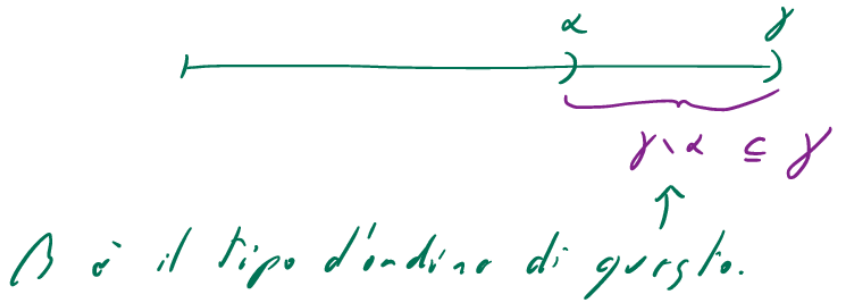
\includegraphics[width = 6.0cm]{immagini/sottrazione_ordinali.png}
\end{figure}

\textcolor{MidnightBlue}{Vediamo ora una dimostrazione formale.}

\begin{proof}
	Vediamo esistenza e unicità separatamente.
	\begin{itemize}
		\item[$\boxed{\text{unicità}}$] Abbiamo l'unicità perché la funzione $+$ è strettamente crescente nel secondo argomento, come visto in precedenza, dunque se ci fosse un altro ordinale diverso da $\beta$, per la totalità dell'ordinamento sugli
		ordinali, sarebbe $<$ o $>$ di $\beta$, da cui anche la somma sarebbe strettamente minore o maggiore e quindi diversa da $\gamma$, pertanto $\beta$ è unico.
		\item[$\boxed{\text{esistenza}}$] Se $\alpha = \gamma$ è sufficiente prendere $\beta = 0$. Possiamo quindi supporre che $\alpha < \gamma$ e consideriamo
		il minimo $\delta$ tale che la somma supera $\gamma$, $\gamma < \alpha + \delta$ - $\delta$ esiste poiché $\gamma \;\textcolor{red}{<}\; s(\gamma) \leq \alpha + s(\gamma)$ e quindi l'insieme degli ordinali la cui somma con $\alpha$ a sinistra è maggiore strettamente di $\gamma$ è non vuoto.\\
		Se $\delta$ è successore, $\delta = \beta + 1$, allora, per la minimalità di $\delta$, si ha $\alpha + \beta \leq \gamma < s(\alpha + \beta) = \alpha + s(\beta) = \alpha + \delta$, pertanto nella prima disuguaglianza non può valere il minore stretto, perché se così fosse si avrebbe che $\gamma \geq s(\alpha + \beta) = \alpha + \delta$, che è assurdo, 
		quindi abbiamo proprio che $\alpha + \beta = \gamma$.\\
		Osserviamo ora che $\delta$ non non può essere limite e così abbiamo concluso. Se $\delta$ fosse limite avremmo:
		\[ \gamma \overset{\text{def. $\delta$}}{<} \alpha + \delta \overset{\text{def. +}}{=} \sup_{\varepsilon < \delta}(\alpha + \varepsilon)
			\] 
		ma allora, dovendo essere il sup di un insieme non vuoto, ciò vuol dire, affinché la disuguaglianza scritta sia vera, che esiste $\varepsilon < \delta$ tale che $\gamma < \alpha + \varepsilon$, contro la minimalità di $\delta$, che è assurdo. Alternativamente,
		ci bastava osservare che, per la minimalità di $\delta$, $\alpha + \varepsilon \leq \gamma$, per ogni $\varepsilon < \delta$, per cui passando la disuguaglianza al sup, avremmo ottenuto $\sup_{\varepsilon < \delta}(\alpha + \varepsilon) \leq \gamma$, che unito alla catena sopra ci dà ancora una volta un assurdo.\footnote{Il passaggio delle disuguaglianze larghe al sup è conseguenza del lemma visto ad inizio capitolo sulle disuguaglianze tra sup.}\,\footnote{L'esistenza può essere dimostrata in modo equivalente per induzione transfinita.}
	\end{itemize}
\end{proof}

\pagebreak

\begin{lemma}[Divisione euclidea di ordinali]
	Dati $\alpha,\gamma \in \Ord$, con $\alpha \ne 0$, esistono e \textcolor{red}{sono unici} $\beta, \rho \in \Ord$ tali che $\rho < \alpha$ e $\alpha \cdot \beta + \rho = \gamma$.
\end{lemma}

\begin{proof}
	Verifichiamo esistenza e unicità separatamente.
	\begin{itemize}
		\item[$\boxed{\text{unicità}}$] Fissato $\beta$, $\rho$ è unico, o per monotonia stretta nella seconda componente della somma o per il lemma sulla sottrazione visto sopra\footnote{Di fatto, essendo che l'unicità nella sottrazione la si ha come conseguenza della monotonia stretta nella seconda componente, il motivo per cui si ha unicità è sempre la monotonia della somma.}.
		Dobbiamo quindi dimostrare solo l'unicità di $\beta$. Supponiamo per assurdo di avere $\beta \ne \beta'$, e WLOG $\beta < \beta'$, con relativamente resti $\rho,\rho' < \alpha$, per cui $\alpha \cdot \beta + \rho = \alpha \cdot \beta' + \rho'$, allora sfruttando la monotonia si ottiene:
		\begin{align*}
			\alpha \cdot \beta +\rho  & \;\textcolor{red}{<}\; \alpha \cdot \beta + \alpha \\
									  & = \alpha \cdot s(\beta) &&\text{(def. ricorsiva $\cdot$)} \\
									  & \leq \alpha \cdot \beta' &&(\beta < \beta')\\
									  & \leq \alpha \cdot \beta' + \rho' &&(\rho' \geq 0)\\
									  & = \alpha \cdot \beta + \rho \quad \textcolor{red}{\lightning} &&(\text{Hp. assurda})
		\end{align*}
		\item[$\boxed{\text{esistenza}}$] Procediamo come nella dimostrazione del lemma di sottrazione, e consideriamo il minimo $\delta$ tale che $\gamma < \alpha \cdot \delta$ - tale $\delta$ esiste, cioè l'insieme è non vuoto, in quanto $\gamma = 1 \cdot \gamma \leq \alpha \cdot \gamma < \alpha \cdot s(\gamma)$.
		Assumiamo che $\delta$ sia successore, $\delta = s(\beta)$, allora per la minimalità di $\delta$, si ha $\alpha \cdot \beta \leq \gamma$\footnote{Notare che non vale necessariamente l'uguale come nella dimostrazione del lemma di sottrazione perché, supponendo il minore stretto, qui avremmo
		$\gamma \geq s(\alpha \cdot \beta) \ne \alpha \cdot \beta + \beta =  \alpha \cdot s(\beta) =\alpha \cdot \delta$.}, possiamo quindi applicare il lemma di sottrazione ordinale ed ottenere l'unico $\rho$ per cui:
		\[ \alpha \cdot \beta + \rho = \gamma
			\]
		Osserviamo ora che $\rho < \alpha$, infatti, se per assurdo fosse $\rho \geq \alpha$, avremmo:
		\begin{align*}
			\gamma & \;\textcolor{red}{<} \; \alpha \cdot \delta \\
				   & = \alpha \cdot s(\beta) \\
				   & = \alpha \cdot \beta + \alpha \\
				   & \leq \alpha \cdot \beta + \rho = \gamma \quad \textcolor{red}{\lightning}
		\end{align*}
		Infine dobbiamo verificare che $\delta$ non sia limite, se per assurdo lo fosse, avremmo:
		\[ \gamma < \alpha \cdot \delta = \sup_{\varepsilon < \delta} (\alpha \cdot \varepsilon)
			\]
		dove, affinché la disuguaglianza sia valida, il sup al RHS deve essere ben definito, e per un insieme di ordinali lo è, come abbiamo visto, quando l'insieme è non vuoto,
		per cui esiste $\varepsilon < \delta$ tale per cui $\gamma < \alpha \cdot \varepsilon$, contro la minimalità di $\delta$, che è assurdo.\\
		Alternativamente si può osservare che, per la minimalità di $\delta$, $\forall \varepsilon < \delta \; \alpha \cdot \varepsilon \leq \gamma$, tale disuguaglianza passa al sup,
		ed aggiunta in fondo alla catena scritta sopra ci dà nuovamente un assurdo.
	\end{itemize}
\end{proof}

\subsection{La forma normale di Cantor}

\begin{theorem}[Forma normale di Cantor - CNF]
	Ogni ordinale $\alpha$ può essere espresso in maniera unica come somma \textcolor{red}{finita} del tipo:
	\[ \alpha = \omega^{\beta_1} \cdot k_1 + \omega^{\beta_2} \cdot k_2 + \ldots + \omega^{\beta_n} \cdot k_n
		\]
	con $\beta_1 > \beta_2 > \ldots > \beta_n$ ordinali, $k_1,k_2,\ldots,k_n \in \omega\setminus\{0\}$ e $n \in \omega$.
\end{theorem}

\begin{proof}
	Dividiamo la dimostrazione in esistenza ed unicità.
	\begin{itemize}
		\item[$\boxed{\text{esistenza}}$] Procediamo per induzione transfinita, supponiamo che ogni ordinale strettamente più piccolo di $\alpha$ abbia una forma normale e verifichiamo che anche $\alpha$ la abbia.\\
		Sia $\gamma$ il minimo tale che $\alpha < \omega^\gamma$ - che esiste in quanto $\alpha \leq \omega_\alpha < \omega^{s(\alpha)}$, dove la prima disuguaglianza è il fatto che $x \mapsto \omega^x$ è una funzione strettamente crescente tra buoni ordini.
		Come nei lemmi precedenti, diamo per buono che $\gamma$ sia successore, $\gamma = s(\beta)$, allora abbiamo che $\omega^\beta \leq \alpha$, possiamo fare la divisione euclidea di $\alpha$ per $\omega^\beta$ e ottenere:
		\[ \alpha = \omega^\beta \cdot k + \rho \qquad \rho < \omega^\beta \leq \alpha
			\]
		con $k$ e $\rho$ unici. A questo punto vale l'ipotesi induttiva per $\rho$ e lo si può scrivere in CNF, per verificare che allora anche $\alpha$ sia scritto in CNF è necessario osservare due cose. In primis che $0 < k < \omega$, infatti:
		\begin{itemize}
			\item \textbf{\underline{$k = 0$}}: in questo caso $\alpha = \rho < \alpha \; \lightning$.
			\item \textbf{\underline{$k \geq \omega$}}: in questo caso $\alpha \;\textcolor{red}<\;\omega^\gamma = \omega^{s(\beta)} = \omega^\beta \cdot \omega \leq \omega^\beta \cdot k \leq \omega^\beta \cdot k + \rho = \alpha \; \lightning$.
		\end{itemize}
		Osserviamo inoltre che, dato che $\rho < \omega^\beta$, scrivendo, con l'ipotesi induttiva, $\rho = \omega^{\beta_2} \cdot k_2 + \ldots + \omega^{\beta_n} \cdot k_n$, si ha $\beta_2 < \beta$, infatti, se così non fosse, cioè se fosse che $\beta_2 \geq \beta$, avremmo:
		\[ \omega^\beta \leq \omega^{\beta_2} \leq \omega^{\beta_2} \cdot k_2 + \ldots + \omega^{\beta_n} \cdot k_n = \rho \;\textcolor{red}<\; \omega^\beta \; \textcolor{red}\lightning
			\]
		pertanto la scrittura ottenuta dalla divisione di $\alpha$ per $\omega^\beta$ è effettivamente una scrittura di $\alpha$ in forma normale di Cantor.\\
		Ci resta soltanto da verificare che il $\gamma$ usato all'inizio non è limite, se per assurdo lo fosse, avremmo:
		\[ \alpha < \omega^\gamma = \sup_{\delta < \gamma} \omega^\delta
			\]
		e affinché la disuguaglianza sia vera il sup al RHS deve essere ben definito, e lo è a condizione che l'insieme di ordinali su cui è preso è non vuoto, ovvero a condizione che esista $\delta < \gamma$ tale che $\alpha < \omega^\delta$, contro la minimalità di $\gamma$.\footnote{Come al
		solito si può osservare alternativamente anche che la disuguaglianza $\omega^\delta \leq \alpha$, valida per la minimalità di $\gamma$, passa al sup generando ancora una volta un assurdo.}
		\item[$\boxed{\text{unicità}}$] Sia $\alpha$ minimo ordinale che non ha un'unica forma normale\footnote{Lo possiamo prendere perché abbiamo visto che la classe degli ordinali è bene ordinata.}, per cui abbiamo che $\alpha$ si può scrivere in almeno due forme normali di Cantor distinte:
		\[ \begin{split}
			\alpha &= \omega^{\beta_1} \cdot k_1 + \omega^{\beta_2} \cdot k_2 + \ldots + \omega^{\beta_n} \cdot k_n \\
				   &= \omega^{\beta_1'} \cdot k_1' + \omega^{\beta_2'} \cdot k_2' + \ldots + \omega^{\beta_{n'}'} \cdot k_{n'}'
		\end{split}
			\]
		dove $n'$ non è necessariamente uguale ad $n$, per cui le scritture possono avere lunghezza diversa.
		Ci basta dimostrare che $\beta_1 = \beta_1'$ e $k_1 = k_1'$, infatti in tal caso, per la stretta monotonia otteniamo:
		\[ \omega^{\beta_2} \cdot k_2 + \ldots + \omega^{\beta_n} \cdot k_n = \omega^{\beta_2'} \cdot k_2' + \ldots + \omega^{\beta_{n'}'} \cdot k_{n'}' \;\textcolor{purple}{<\;\omega^{\beta_1},\omega^{\beta_1'}} 
			\]
		dunque avremmo trovato un ordinale strettamente più piccolo di $\alpha$ con almeno due scritture distinte in CNF e quindi avremmo un assurdo.\\
		Se abbiamo che $\beta_1 = \beta_1'$, allora necessariamente anche $k_1 = k_1'$, infatti in questo caso possiamo scrivere:
		\[ \alpha = \omega^{\beta_1} \cdot k_1 + \underbrace{\ldots}_{\textcolor{purple}{< \omega^{\beta_1}}} = \omega^{\beta_1} \cdot k_1' + \underbrace{\ldots}_{\textcolor{purple}{< \omega^{\beta_1}}}
			\]
		cioè nella forma della divisione euclidea, e quindi otteniamo $k_1 = k_1'$, per unicità della scrittura in questa forma\footnote{Inoltre otterremo anche che le code sono uguali, ma di nuovo ciò è di fatto sempre una conseguenza della monotonia stretta sulla seconda componente.}.\\
		Ci resta quindi solo da verificare che $\beta_1 = \beta_1'$, se per assurdo supponessimo, WLOG, che $\beta_1 < \beta_1'$, dunque $s(\beta_1) \leq \beta_1'$, avremmo:
		\[ \alpha = \omega^{\beta_1} \cdot k_1 + \omega^{\beta_2} \cdot k_2 + \ldots + \omega^{\beta_n} \cdot k_n \; \textcolor{purple}{<\; \omega^{s(\beta_1)}} \leq \omega^{\beta_1'} \cdot k_1' + \ldots = \alpha \; \textcolor{red}\lightning
			\]
	\end{itemize}
\end{proof}

\begin{exercise}
	Dimostrare le disuguaglianza in \textcolor{purple}{viola} (sono tutte uguali).
\end{exercise}

\begin{soln}
	Per l'ultima disuguaglianza basta osservare che per monotonia:
	\[ \omega^{\beta_1} \cdot k_1 + \omega^{\beta_2} \cdot k_2 + \ldots + \omega^{\beta_n} \cdot k_n \leq \omega^{\beta_1} \cdot k_1 + \omega^{\beta_{\textcolor{red}1}} \cdot k_2 + \ldots + \omega^{\beta_{\textcolor{red}1}} \cdot k_n = \omega^{\beta_1} \cdot (\underbrace{k_1 + \ldots + k_n}_{=: k})
		\]
	e a questo punto $\omega^{\beta_1} \cdot k \;\textcolor{red}{<}\; \omega^{\beta_1} \cdot \omega = \omega^{s(\beta_1)}$. Per le prime tre disuguaglianze, basta ragionare in maniera identica con $\omega^{\beta_2} \cdot k_2 + \ldots + \omega^{\beta_n} \cdot k_n$ (analogamente con la versione con i $'$), ottenendo
	$\omega^{\beta_2} \cdot k \;\textcolor{red}{<}\; \omega^{\beta_2} \cdot (k + 1) \leq \omega^{s(\beta_2)} \leq \omega^{\beta_1}$.
\end{soln}

\subsection{Punti fissi e \texorpdfstring{$\varepsilon$}{epsilon}-numbers}
Si potrebbe credere che il teorema precedente, applicato ricorsivamente agli esponenti $\beta_1,\ldots,\beta_n$, implichi che ogni ordinale
si possa scrivere sotto forma di un'espressione finita composta di somme, prodotti e potenze delle costanti $0,1,2,\ldots,\omega$. Tipo questa:
\[ \omega^{\omega^4 \cdot 7 + \omega^2 \cdot 1}\cdot 9 + \omega^{75} + 9
	\]
Effettivamente, se valesse $\textcolor{red}{\alpha > \beta_1}>\beta_2>\ldots>\beta_n$ per ogni $\alpha$, allora questa conclusione sarebbe corretta.
Però è possibile esibire un ordinale $\varepsilon_0$ - e, in realtà, un'intera classe propria di ordinali come questo - tale che $\varepsilon_0 = \omega^{\varepsilon_0}$\footnote{Notare che in questo caso non vale che $\alpha > \beta_1$, e quindi $\varepsilon_0$ non può essere scritto nella forma sopra.}.
La forma normale di Cantor di $\varepsilon_0$ è quindi, chiaramente, $\omega^{\varepsilon_0}$, e procedere ricorsivamente sull'esponente $\omega^{\omega^{\varepsilon_0}},\omega^{\omega^{\omega^{\varepsilon_0}}}$, etc. non conduce ad un'espressione finita, intuitivamente verrebbe una cosa del tipo:
\[ \varepsilon_0 = \underbrace{\omega^{\omega^{\omega^{\omega^{\iddots}}}}}_{\text{$\omega$ volte}}
	\]
La proposizione seguente è interessante di per sé, ma, in particolare, ci permetterà di dimostrare l'esistenza degli \vocab{$\varepsilon$-numbers}.

\begin{proposition}[Ogni funzione normale ha una classe propria di punti fissi]
	Sia $F : \Ord \rightarrow \Ord$ una funzione classe \textcolor{orange}{strettamente} crescente e continua\footnote{Tali funzioni prendono il nome di \vocab{funzioni normali.}} - ossia $F(\lambda) = \sup F[\lambda] = \sup_{\alpha < \lambda} F(\alpha)$ per $\lambda$ limite.
	Allora, per ogni $\alpha \in \Ord$, $F$ ha un punto fisso $\geq \alpha$, ossia vale che:
	\[ \exists \pi \in \Ord \; \alpha \leq \pi \land F(\pi) = \pi
		\]
\end{proposition}

\begin{proof}
	Fissato $\alpha \in \Ord$ costruiamo un punto fisso di $F$ che sia maggiore o uguale ad $\alpha$. Definiamo per ricorsione numerabile:
	\[ \pi_n := \begin{cases}
		\pi_0 = \alpha \\
		\pi_{n+1} = F(\pi_n)
	\end{cases}
		\]
	se $F(\alpha) = \alpha$ allora $\pi_n = \alpha$ ed abbiamo il punto fisso voluto, altrimenti, essendo $F$ strettamente crescente, si ha $\alpha < F(\alpha)$, cioè $\pi_0 < \pi_1$\footnote{Typo Mamino scrive ovunque 0 al posto di $\alpha$.}, da cui si verifica per induzione che $\pi_n$ è
	strettamente crescente\footnote{Per ipotesi induttiva $\pi_{n-1} < \pi_n$, e poiché $F$ è strettamente crescente, applicandola alla disuguaglianza si ottiene $\pi_n < \pi_{n+1}$, quindi il passo induttivo.}, $\forall n \in \omega \; \pi_n < \pi_{n+1}$, di conseguenza, detto:
	\[ \pi \Mydef \sup_{n \in \omega} \pi_n
		\]
	abbiamo che $\pi$ è un ordinale limite, poiché $\pi \not \in \{\pi_n | n \in \omega\}$ (altrimenti non sarebbe il sup), inoltre naturalmente $\pi > \pi_0 = \alpha$, per cui:
	\[ F(\pi) \overset{\text{$F$ continua}}{=} \sup_{n \in \omega} F(\pi_n) \overset{\text{def}}{=} \sup_{n \in \omega} \pi_{n+1} = \pi
		\]
\end{proof}

\begin{remark}[I punti fissi sono una classe propria di ordinali]
	Abbiamo dimostrato che per ogni ordinale c'è un punto fisso di $F$ (sotto opportune ipotesi) che è maggiore di tale ordinale, pertanto i punti fissi di $F$ non possono formare un insieme di ordinali perché non esiste un estremo superiore,
	dunque formano una (sotto)classe propria di $\Ord$.
\end{remark}

\begin{example}[$x \mapsto \omega^x$]
	La mappa $x \mapsto \omega^x$ è strettamente crescente, per la monotonia stretta dell'esponenziale nella seconda componente, ed è continua in quanto abbiamo definito l'esponenziale di ordinali infiniti estendendo per continuità la definizione dal caso finito,
	pertanto per il teorema sopra tale mappa ha una classe propria di punti fissi, che sono appunto tali per cui $\varepsilon = \omega^{\varepsilon}$.
\end{example}

\begin{exercise}
	Sia $\varepsilon_0 = \sup\{1,\omega,\omega^{\omega},\omega^{\omega^{\omega}}, \omega^{\omega^{\omega^{\omega}}},\ldots\}$. Formalmente definiamo per ricorsione numerabile $\alpha_0 = 1$, $\alpha_{n+1}=\omega^{\alpha_n}$,
	allora $\varepsilon_0 = \sup\{\alpha_n | n \in \omega\}$. Dimostrare che $\varepsilon_0$ è il più piccolo punto fisso della funzione $x \mapsto \omega^x$.
\end{exercise}

\begin{soln}
	Osserviamo in primis che $\varepsilon_0$ è un ordinale limite, per farlo ci basta osservare che $\varepsilon_0 \not \in \{\alpha_n | n \in \omega\}$, infatti la successione $\alpha_n$ è strettamente crescente, dunque se fosse che $\varepsilon_0 = \alpha_m$, per $m \in \omega$,
	allora $\alpha_{m+1} > \varepsilon_0$ e quindi quest'ultimo non sarebbe il sup, che è assurdo, segue quindi che $\varepsilon_0$ è limite per un lemma visto.\footnote{In realtà non serve osservarlo per poter applicare il lemma di commutazione tra potenze e sup di insiemi di ordinali, ma è comunque interessante notarlo.}\\
	Verifichiamo ora che $\varepsilon_0$ è un punto fisso di $x \mapsto \omega^x$:
	\[ \varepsilon_0 \overset{\text{def.}}{=} \sup_{n \in \omega} \alpha_n \overset{(\star)}{=} \sup_{n \in \omega} \omega^{\alpha_n} \overset{\text{lemma}}{=} \omega^{\sup_{n \in \omega} \alpha_n} \overset{\text{def.}}{=} \omega^{\varepsilon_0}
		\]
	dove $(\star)$ vale per il lemma della disuguaglianza dei sup applicato in ambo i versi, infatti dato $\alpha_n$, è sufficiente prendere $\omega^{\alpha_n}$ nel secondo insieme per avere la prima disuguaglianza, viceversa, preso $\omega^{\alpha_n}$ nel secondo, basta osservare che $\alpha_{n+1} = \omega^{\alpha_n}$ è nel primo.\\
	Infine osserviamo che $\varepsilon_0$ è il più piccolo punto fisso di $x \mapsto \omega^x$, infatti, se esistesse $y < \varepsilon_0$ punto fisso di $x \mapsto \omega^x$, allora avremmo:
	\[ \alpha_n \leq y < \alpha_{n+1}\,\footnote{Il caso $y \in \omega$ andrebbe fatto a parte per essere precisi, ma è molto facile osservare che anche in questo caso segue la tesi.}
		\]
	infatti $y \in \bigcup_{n+1}\alpha_n$, dunque $y$ è almeno in un $\alpha_n$ che è successore (altrimenti basta prendere il successivo), e ci basta prendere il minimo successore a cui appartiene per avere la disuguaglianza sopra (se il termine di testa di $y$ in CNF non fosse $\geq \alpha_n$, allora $\alpha_{n+1}$ non sarebbe il minimo a cui appartiene $y$).
	Dalle disuguaglianze sopra segue che:
	\[ \alpha_{n+1} = \omega^{\alpha_n} \leq \omega^y \leq \omega^{\alpha_{n+1}} = \alpha_{n+2}
		\]
	per cui se $y$ fosse un punto fisso, si avrebbe $y < \alpha_{n+1} \leq \omega^y = y \; \lightning$.
\end{soln}

\begin{exercise}[Lista dei punti fissi di una funzione normale]
	Sia $F : \Ord \rightarrow \Ord$ crescente e continua, allora esiste $G : \Ord \rightarrow \Ord$ strettamente crescente tale che:
	\[ \forall \alpha \in \Ord \; F(\alpha) = \alpha \leftrightarrow \exists \beta \in \Ord \; \alpha = G(\beta)
		\]
\end{exercise}

\begin{soln}
	Dalla proposizione sopra abbiamo visto che i punti fissi di $F : \Ord \to \Ord$ sono una classe propria $C_F$, dunque possiamo definire per ricorsione transfinita:
	\[ G(\alpha) = \min\{x \in C_F : \forall y \in G[\alpha] \; x > y\}\,\footnote{Non stiamo usando separazione, è solo una formula insiemistica, e il minimo è sempre ben definito perché la classe $C_F$ è una sottoclasse di $\Ord$ che è bene ordinata, e $C_F$ è sempre non vuota perché è una classe propria.}
		\]
	che è ben definita per il teorema di ricorsione transfinita, ed è strettamente crescente per costruzione. Verifichiamo inoltre che $\Imm(G) = C_F$, preso $\beta \in C_F$, si ha che:
	\[ \beta < s(\beta) \leq G(s(\beta))
		\]
	ed essendo $G(s(\beta))$ il più piccolo ordinale in $C$ più grande di tutti gli ordinali di $G[s(\beta)]$, per minimalità, si ha che esiste $\gamma \in G[s(\beta)]$ tale che $\gamma \geq \beta$, da cui $\beta \in G[s(\beta)]$, e quindi $\beta \in \Imm(G)$.
	Segue quindi che $G$ è un isomorfismo tra $\Ord$ e $C_F \subseteq \Ord$, ed in tal modo soddisfa la tesi, infatti $\forall \alpha \in \Ord \; F(\alpha) = \alpha \iff \alpha \in C_F \overset{\text{$G$ surg.}}{\iff} \exists \beta \in C_F \; G(\beta) = \alpha$.
\end{soln}

\begin{exercise}[Unicità della lista]
	La $G$ dell'esercizio precedente è univocamente determinata da $F$ ed è una funzione classe continua.
\end{exercise}

\begin{soln}
	Verifichiamo che data $H : \Ord \to C_F \subseteq \Ord$ strettamente crescente e che soddisfi la proprietà $\forall \alpha \in \Ord \; F(\alpha) = \alpha \leftrightarrow \exists \beta \in \Ord \; \alpha = H(\beta)$ (che equivale al fatto che $\Imm(H) = C_F$,
	ovvero $H$ isomorfismo tra $\Ord$ e $C_F$, la classe propria dei punti fissi di $F$), allora soddisfa la definizione ricorsiva di $G$ data nell'esercizio precedente,
	e quindi coincide proprio con quest'ultima per il teorema di ricorsione transfinita, da cui segue quindi l'unicità della lista dei punti fissi $G$.\\
	Poiché $H$ è strettamente crescente per ipotesi, naturalmente $H(\alpha)$ è più grande di tutti gli elementi di $H[\alpha]$, inoltre,
	se esistesse $\gamma \in C_F$, tale che $\gamma < H(\alpha)$ e maggiore di tutti gli $H[\alpha]$, allora $\gamma > F(\delta)$ per $\delta < \alpha$, per la monotonia di $H$, e $\gamma < F(\delta)$ per $\delta \geq \alpha$, dunque $\gamma \not\in \Imm(H)$, che è per ipotesi contro la surgettività di $H : \Ord \to C_F$,
	dunque $H(\alpha)$ è proprio il più piccolo ordinale di $C_F$ più grande di tutti gli ordinali in $H[\alpha]$, pertanto $H$ soddisfa la relazione ricorsiva di $G$ e quindi coincide con quest'ultima.\\
	La continuità di $G$ segue banalmente dalla definizione ricorsiva che abbiamo dato, infatti:
	\[ G(\lambda) = \min\{x \in C_F : \forall y \in G[\lambda] \; x > y\} = \sup G[\lambda] = \sup_{\alpha < \lambda} G(\alpha)
		\]
\end{soln}

\begin{remark}[Derivata di funzioni ordinali]
	Data una funzione $F : \Ord \to \Ord$ normale la proposizione iniziale ci dice che $F$ ha una classe propria di punti fissi, e gli ultimi due esercizi ci dicono che tali punti fissi possono essere elencata in modo unico e strettamente crescente da una nuova funzione $G : \Ord \to \Ord : \alpha \mapsto \alpha$-esimo punto fisso di $F$,
	tale funzione prende talvolta in letteratura il nome di \vocab{derivata} di $F$. Notare infine che $G$, per quanto abbiamo visto, è, per costruzione, a sua volta normale, dunque può essere ``derivata'' a sua volta, dandoci nuovamente un'unica lista dei suoi punti fissi.
\end{remark}

\begin{definition}[$\varepsilon$-numbers]
	Definiamo l'unica funzione che elenca i punti fissi di $x \mapsto \omega^x$, ovvero la sua derivata, $\varepsilon_\alpha$, i cui valori prendono il nome di \vocab{epsilon-numbers} e sono appunto i punti fissi di $x \mapsto \omega^x$ elencati in maniera ordinata dagli ordinali.
\end{definition}

\begin{definition}[$\zeta$-numbers]
	Definiamo l'unica funzione che elenca i punti fissi della funzione $\varepsilon_\alpha$, ovvero la sua derivata\footnote{Sarebbe la derivata seconda di $x \mapsto \omega^x$.}, $\zeta_\alpha$, i cui valori prendono il nome di \vocab{zeta-numbers} e sono appunto i punti fissi di $\zeta_\alpha$ elencati in maniera ordinata dagli ordinali.
\end{definition}

I primi due esercizi seguenti saranno assai più facili quando, usando l'assioma della scelta, dimostreremo che un insieme numerabile di insiemi numerabili è numerabile.\footnote{Ricordare che l'avevamo già dimostrato dando per buono di avere una successione di enumerazioni,
ma anche il quel caso l'enumerazione ce la si può procurare solo con scelta.}

\begin{exercise}[\textcolor{red}{$\star$ Difficile senza leggere l'idea sotto}]
	$|\varepsilon_0| = \aleph_0$.\footnote{\underline{\textbf{Idea}}: dimostrare che $\alpha \in \varepsilon_0$ se e solo se $\alpha$ può essere scritto a partire da $0,1,\omega$, applicando le operazioni di somma, prodotto, ed esponente ordinale un numero finito di volte.}
\end{exercise}

\begin{soln}
	Per definizione $\varepsilon_0 = \sup\{\alpha_n | n \in \omega\}$, dove $\alpha_0 = 1$ e $\alpha_{n+1}=\omega^{\alpha_n}$, si ha che $\varepsilon_0 \geq \alpha_1 = \omega$, dunque $\omega \subseteq \varepsilon_0 \to \aleph_0 \leq |\varepsilon_0|$.\footnote{Se avessimo AC
	potremmo concludere immediatamente l'altra disuguaglianza dimostrando per induzione che $|\alpha_n| = \aleph_0$, da cui $|\varepsilon_0| = |\sup_{n \in \omega} \alpha_n| = |\bigcup_{n \in \omega} \alpha_n| \overset{\text{AC}}{\leq} \aleph_0$.} Per la
	disuguaglianza opposta
\end{soln}

\begin{exercise}[\textcolor{red}{$\star \star$ Ostico}]
	Sia $\zeta_0$ minimo tale che $\varepsilon_{\zeta_0} = \zeta_0$, allora $|\zeta_0| = \aleph_0$.
\end{exercise}

\begin{soln}
	Per gli esercizi sopra, sappiamo che $\zeta_\alpha$ è la funzione che elenca i punti fissi di $\varepsilon_\alpha$ in maniera strettamente crescente, dunque $\zeta_0$ è il più piccolo punto fisso di $\varepsilon_\alpha$ per definizione.
	Dallo stesso teorema, sappiamo che $\varepsilon_\alpha$, essendo a sua volta successione crescente di punti fissi di $x \mapsto \omega^x$, è strettamente crescente, per cui $\varepsilon_0 \leq \varepsilon_{\zeta_0}$, da cui otteniamo la disuguaglianza dal basso $\aleph_0 = |\varepsilon_0| \leq |\varepsilon_{\zeta_0}|$.\\
	Per il viceversa
\end{soln}

\begin{exercise}[Teorema di scrittura in base ordinale]
	Sia $\gamma$ un qualunque ordinale $\geq 2$. Ogni ordinale $\alpha$ si scrive in modo unico come somma finita:
	\[ \alpha = \gamma^{\beta_1}\cdot k_1 + \ldots \gamma^{\beta_n}\cdot k_n
		\]
	con $\beta_1 > \beta_2 > \ldots > \beta_n$ ordinali, $k_1,\ldots,k_n \in \gamma\setminus\{0\}$ e $n \in \omega$.
\end{exercise}

\begin{soln}
	Dividiamo esistenza ed unicità della scrittura in base $\gamma$.
	\begin{itemize}
		\item[$\boxed{\text{esistenza}}$] Procediamo per induzione transfinita forte, dunque supponiamo che tutti gli ordinali minori strettamente di $\alpha$ si possano scrivere in base $\gamma$ come sopra, e dimostriamo che anche $\alpha$ si può scrivere in tale forma.\\
		Sia $\delta$ il minimo ordinale tale che $\alpha < \gamma^\delta$ - che esiste in quanto $x \mapsto \gamma^x$ è strettamente crescente tra classi bene ordinate, per cui $\alpha \leq \gamma^\alpha < \gamma^{s(\alpha)}$, e quindi la sottoclasse di $\Ord$ da cui prendiamo il minimo è non vuota.
		Assumiamo che $\delta = \beta + 1$, e per minimalità di $\delta$ si ha $\gamma^\beta \leq \alpha$ e applichiamo il lemma di divisione euclidea per ottenere:
		\[ \alpha = \gamma^\beta \cdot k + \rho \qquad \rho < \gamma^\beta \leq \alpha
			\]
		con $k$ e $\rho$ unici. Possiamo applicare l'ipotesi induttiva a $\rho$ e scrivere $\rho = \gamma^{\beta_2}\cdot k_2 + \ldots + \gamma^{\beta_n} \cdot k_n$, a questo punto, per dire che la scrittura trovata dalla divisione sostituendo $\rho$ con la sua scrittura in base $\gamma$,
		è effettivamente una scrittura in base $\gamma$ per $\alpha$, dobbiamo verificare due cose. In primis osserviamo che $0 < k < \gamma$:
		\begin{itemize}
			\item \underline{$k = 0$}: in tal caso $\alpha = \rho < \alpha \; \textcolor{red}\lightning$.
			\item \underline{$k \geq \gamma$}: in questo caso $\gamma^\delta = \gamma^{\beta + 1} = \gamma^\beta \cdot \gamma \leq \gamma^\beta \cdot k \leq \gamma^\beta \cdot k + \rho = \alpha \;\textcolor{red}<\; \gamma^\delta \; \textcolor{red}\lightning$. 
		\end{itemize}
		Osserviamo inoltre che $\beta > \beta_2$, infatti, se fosse $\beta_2 \geq \beta$ si avrebbe:
		\[ \gamma^\beta \leq \gamma^{\beta_2} \leq \gamma^{\beta_2} \cdot k_2 + \ldots + \gamma^{\beta_n} \cdot k_n = \rho \;\textcolor{red}<\; \gamma^{\beta} \quad \textcolor{red}\lightning
			\]
		quindi abbiamo ottenuto che esiste almeno una scrittura in base $\gamma$ per $\alpha$. Ci resta soltanto da verificare l'assunzione iniziale che $\delta$ sia successore e non limite, se $\delta$ fosse limite si avrebbe:
		\[ \alpha < \gamma^\delta = \sup_{\varepsilon < \delta} \gamma^{\varepsilon}
			\]
		affinché la disuguaglianza sia vera l'insieme di ordinali su cui si prende il sup al RHS deve essere non vuoto, cioè deve esistere $\varepsilon < \delta$ tale che $\alpha < \gamma^{\varepsilon}$, contro la minimalità di $\delta$. Alternativamente
		si può osservare che, per la minimalità di $\delta$, si ha $\forall \varepsilon < \delta \; \gamma^{\varepsilon} \leq \alpha$, e, passando questa disuguaglianza al sup - cosa che si può fare per il lemma sulla disuguaglianza dei sup - si ottiene $\gamma^\delta = \sup_{\varepsilon < \delta} \gamma^{\varepsilon} \leq \alpha \; \textcolor{red}\lightning$.
		\item[$\boxed{\text{unicità}}$] Sia $\alpha$ il minimo ordinale che non si scrive in modo unico in base $\gamma$ - se la sottoclasse di tali ordinali fosse vuota avremmo già la tesi - ovvero:
		\begin{align*}
			\alpha &= \gamma^{\beta_1}\cdot k_1 + \ldots \gamma^{\beta_n}\cdot k_n \\
				   &= \gamma^{\beta_1'}\cdot k_1' + \ldots \gamma^{\beta_n'}\cdot k_n'
		\end{align*}
		Osserviamo che se $\beta_1 = \beta_1'$ e $k_1 = k_1'$, allora per la stretta monotonia della somma sulla seconda componente si ottiene:
		\[ \gamma^{\beta_2}\cdot k_2 + \ldots \gamma^{\beta_n}\cdot k_n = \gamma^{\beta_2}\cdot k_2 + \ldots \gamma^{\beta_n}\cdot k_n < \alpha
			\]
		ovvero che esiste un ordinale più piccolo di $\alpha$ che ammette due scritture in base $\gamma$, contro la minimalità di $\alpha$. Osserviamo inoltre che se $\beta_1 = \beta_1'$,
		allora necessariamente $k_1 = k_1'$, infatti:
		\[ \alpha = \gamma^{\beta_1}\cdot k_1 + \underbrace{\ldots}_{<\gamma^{\beta_1}} = \gamma^{\beta_1'} \cdot k_1' + \underbrace{\ldots}_{<\gamma^{\beta_1'}} 
			\]
		dunque $k_1 = k_1'$ e c'è uguaglianza delle code per unicità data dal lemma di divisione.
		Verifichiamo infine che necessariamente $\beta_1 = \beta_1 '$, infatti, se fosse WLOG $\beta_1 < \beta_1'$, cioè si avrebbe:
		\[ \alpha = \gamma^{\beta_1}\cdot k_1 + \ldots \gamma^{\beta_n}\cdot k_n \leq \gamma^{\beta_1} \cdot k \;\overset{\textcolor{purple}{k < \gamma}}{<}\; \gamma^{s(\beta_1)} \leq \gamma^{\beta_1 '} \leq \gamma^{\beta_1'}\cdot k_1' + \ldots \gamma^{\beta_n'}\cdot k_n' = \alpha \; \textcolor{red}\lightning
			\]
		dove abbiamo posto $k = k_1 + \ldots + k_n$.
	\end{itemize}
\end{soln}

\subsection{Operazioni in forma normale di Cantor}
È facile ridurre l'aritmetica ordinale, in forma normale di Cantor, ad una piccola collezione di regole meccaniche.
Nel contesto del corso, queste regole hanno un'importanza limitata, è però utile sapere che ci sono, ed avere un'idea del loro aspetto.
Il lemma seguente è un caso particolare, ma è semplice e vale la pena ricordarlo.

\begin{lemma}[Assorbimento a sinistra da parte dell'ordinale più grande]
	Siano $\alpha,\beta,\gamma \in \Ord$ tali che $\alpha < \omega^{\beta} \leq \gamma$, allora:
	\[ \alpha + \textcolor{orange}{\gamma} = \textcolor{orange}{\gamma}
		\]
\end{lemma}

\textcolor{MidnightBlue}{Ciò calcolare $\alpha + \gamma$ assorbe tutti gli $\alpha$ abbastanza piccoli, ossia quelli minori di qualche potenza di $\omega$ che sia a sua volta minore o uguale a $\gamma$.}

\begin{proof}
	Naturalmente si ha che $\gamma \leq \alpha + \gamma$ (debole monotonia sulla prima componente) dunque ci basta dimostrare che $\alpha + \gamma \leq \gamma$.
	Scrivendo $\alpha$ in forma normale di Cantor abbiamo:
	\[ \alpha = \omega^{\beta_1} \cdot k_1 + \ldots + \omega^{\beta_n} \cdot k_n
		\]
	con $\beta_1 > \beta_2 > \ldots > \beta_n$. Quindi possiamo ottenere che $\alpha \leq \omega^{\beta_1} \cdot k$, per qualche $k \in \omega$, infatti, sostituendo tutti gli esponenti $\alpha_2,\ldots,\alpha_n$ con $\alpha_1$, ed usando la debole monotonia, si ottiene:
	\[ \alpha = \omega^{\beta_1} \cdot k_1 + \ldots + \omega^{\beta_n} \cdot k_n \leq \alpha = \omega^{\beta_1} \cdot k_1 + \omega^{\beta_{\textcolor{red}{1}}} \cdot k_2 + \ldots + \omega^{\beta_{\textcolor{red}{1}}} \cdot k_n = \omega^{\beta_1}\cdot (k_1 + \ldots + k_n)
		\]
	per cui poniamo $k := k_1 + \ldots + k_n$\footnote{Una volta viste le regole per la somma in forma normale anziché questa stima sarà più comodo e veloce sommare $\omega^{\alpha_1}$ in fondo ed ottenere la stima $\alpha \leq \omega^{\alpha} \cdot (k_1 + 1)$, che è anche migliore.}.
	Osserviamo che $\beta_1$ è il più piccolo esponente per cui si ha tale disuguaglianza (qualsiasi cosa più piccola ci dà per monotonia $\alpha < \alpha$), mettendo assieme ciò con l'ipotesi $\alpha < \omega^\beta$, deduciamo $\beta_1 < \beta$, da cui
	quindi $\beta_1 + 1 \leq \beta$. Usando il lemma della sottrazione, possiamo sottrarre $\omega^{\beta_1 + 1}$ a $\gamma$ e ottenere $\gamma = \omega^{\beta_1 + 1} + \gamma' = \omega^{\beta_1} \cdot \omega + \gamma'$, con $\gamma'$ unico per il lemma.
	Da cui:
	\[ \textcolor{green}{\alpha} + \textcolor{purple}{\gamma} \overset{\text{sopra + monotonia}}{\leq} \textcolor{green}{\omega^{\beta_1} \cdot k} + \textcolor{purple}{\omega^{\beta_1} \cdot \omega + \gamma'} = \omega^{\beta_1} (k + \omega) + \gamma' \;\textcolor{red}{=}\; \omega^{\beta_1} \cdot \omega + \gamma' = \gamma
		\]
	dove l'uguaglianza in \textcolor{red}{rosso} segue deriva dal fatto che:
	\[ k + \omega = \sup\{k + n | n < \omega\} = \omega
		\]
\end{proof}

\begin{proposition}[Regole di calcolo in forma normale di Cantor]
	Per le somme ($c \ne 0$, $d \ne 0$) vale che:
	\[ \omega^{\alpha} \cdot c + \omega^\beta \cdot d = \begin{cases}
		\omega^\beta \cdot d &\text{se $\alpha < \beta$} \\
		\omega^\alpha \cdot (c + d) &\text{se $\alpha = \beta$} \\
		\omega^{\alpha} \cdot c + \omega^\beta \cdot d &\text{se $\beta < \alpha$}
	\end{cases}
		\]
	Per i prodotti si applica la proprietà distributiva, e poi le regole seguenti:
	\begin{align*}
		\beta > 0 \rightarrow (\omega^{\alpha_1} \cdot k_1 + \ldots \omega^{\alpha_2} \cdot k_2 + \ldots) \cdot \omega^{\beta} &= \omega^{\alpha_1 + \beta} \\
		n \in \omega\setminus\{0\} \rightarrow (\omega^{\alpha_1} \cdot k_1 + \ldots \omega^{\alpha_2} \cdot k_2 + \ldots) \cdot n &= \omega^{\alpha_1} \cdot k_1\textcolor{red}{n} + \ldots \omega^{\alpha_2} \cdot k_2 + \ldots
	\end{align*}
	Per le potenza si usano $\alpha^{\beta + \gamma} = \alpha^\beta \cdot \alpha^\gamma$ e $\alpha^{\beta \cdot n} = (\alpha^\beta)^n$, poi:
	\begin{align*}
		k \in \omega\setminus\{0\}\qquad\qquad k^{\omega^{1 + \alpha}} &= \omega^{\omega^{\alpha}} \\
		\beta > 0 \land \alpha_1 > 0 \rightarrow (\omega^{\alpha_1} \cdot k_1 + \ldots \omega^{\alpha_2} \cdot k_2 + \ldots)^{\omega^\beta} &= \omega^{\alpha_1 \cdot \omega^\beta}
	\end{align*}
\end{proposition}

\begin{proof}
	La regole per la somma sono immediate: la prima è il lemma precedente, infatti se $\alpha < \beta$, allora $\omega^\alpha \cdot c < \omega^\alpha \cdot \omega = \textcolor{purple}{\omega^{s(\alpha)}} \leq \omega^{\beta} \cdot d$, e il termine di sinistra viene assorbito nella somma;
	la seconda è la proprietà distributiva a sinistra valida per il prodotto di ordinali in generale, e la terza è la scrittura stessa in forma normale di Cantor, che per ipotesi non può essere semplificata ulteriormente.
	Per dimostrare che:
	\[ \textcolor{purple}{\beta > 0 \rightarrow (\omega^{\alpha_1}\cdot k_1 + \omega^{\alpha_2} \cdot k_2 + \ldots) \cdot \omega^{\beta} = \omega^{\alpha_1 + \beta}}
		\]
	osserviamo preliminarmente il caso particolare $n \cdot \omega = \omega$ per $n \in \omega\setminus\{0\}$:
	\[ \omega \leq n \cdot \omega = \sup\{n \cdot i | i \in \omega\} \leq \sup\{j | j \in \omega\} = \omega
		\]
	dove la prima disuguaglianza è la solita debole monotonia sulla prima componente del prodotto, la seconda disuguaglianza è il lemma sulla disuguaglianza dei sup e vale perché l'insieme di destra contiene tutti i naturali e quindi tutti i prodotti,
	infine, l'ultima uguaglianza è semplicemente il fatto che $\omega$ è limite e quindi uguale al sup dei suoi elementi.
	Ora possiamo scrivere $\beta = 1 + \gamma$ (volendo è il lemma della sottrazione ordinale, ma può essere giustificato in tanti altri modi), per cui si ha:\footnote{Typo Mamino, c'è proprio uguaglianza al quarto passaggio.}
	\[ \begin{split}
		\textcolor{orange}{\omega^{\alpha_1 + \beta}} &= \omega^{\alpha_1}\omega^\beta \\
								  &\leq \textcolor{MidnightBlue}{(\omega^{\alpha_1} \cdot k_1 + \omega^{\alpha_2} \cdot k_2 + \ldots) \cdot \omega^{\beta}} \\
								  &\leq (\omega^{\alpha_1} \cdot k_1 + \omega^{\alpha_2} \cdot k_2 + \ldots + \textcolor{red}{\omega^{\alpha_1}}) \cdot \omega^{\beta} \\
								  &= \omega^{\alpha_1}(k_1+1)\cdot \omega^{\beta} \\
		   						  &= \omega^{\alpha_1}\underbrace{(k_1 + 1)\omega}_{=\omega}\omega^{\gamma}\\
		   						  &= \omega^{\alpha_1} \cdot \omega \cdot \omega^{\gamma} = \textcolor{orange}{\omega^{\alpha_1 + \beta}}
 	\end{split}
		\]
	dove: la prima uguaglianza sono le proprietà delle potenze degli ordinali; la seconda disuguaglianza è la debole monotonia della prima componente del prodotto; nella terza abbiamo aggiunto $\omega^{\alpha_1}$ alla fine,
	ed è la stretta monotonia sulla seconda componente della somma, essendo $0 < \omega^{\alpha_1}$, unita alla debole monotonia sulla prima componente del prodotto totale, da cui la disuguaglianza larga; la quarta uguale è la regola della somma, infatti per l'ipotesi sulla forma normale di Cantor,
	avendo aggiunto $\omega^{\alpha_1}$ alla fine, i termini vengono cancellati, si ottiene $\omega^{\alpha_1} \cdot k_1 + \omega^{\alpha_1}$ e infine si usa la distributività a sinistra;
	per la quinta uguaglianza stiamo usando che $\beta = 1 + \gamma$ e le solite proprietà delle potenze; la sesta uguaglianza è il caso particolare visto sopra $n \cdot \omega = \omega$, e naturalmente $k_1 + 1 \in \omega$; infine, nell'ultima uguaglianza usiamo ancora che $\beta = 1 + \gamma$.\\
	La seconda regola, del prodotto di un ordinale in forma normale e un naturale:
	\[ \textcolor{purple}{n \in \omega\setminus\{0\} \rightarrow (\omega^{\alpha_1} \cdot k_1 + \ldots \omega^{\alpha_2} \cdot k_2 + \ldots) \cdot n = \omega^{\alpha_1} \cdot k_1\textcolor{red}{n} + \ldots \omega^{\alpha_2} \cdot k_2 + \ldots}
		\]
	si ottiene per induzione su $n$. La prima per il prodotto invece è immediata:
	\[ \begin{split}
		\textcolor{purple}{k^{\omega^{1+\alpha}}} &= k^{\omega \cdot \omega^{\alpha}} \\
												  &= (k^{\omega})^{\omega^{\alpha}} \\
												  &= (\sup\{k^{n} | n \in \omega\})^{\omega^{\alpha}} \\
												  &= \omega^{\omega^{\alpha}}
		\end{split}
		\]
	sono solo la definizione ricorsiva della potenza nel caso limite e le proprietà delle potenze degli ordinali, l'unica cosa degna di nota da osservare è che l'estremo superiore di quell'insieme,
	per il solito lemma, maggiora $\{n | n \in \omega\}$, e contemporaneamente $\omega$ è un suo maggiorante per questo motivo si vede che è $\omega$ stesso.\\
	Per dimostrare infine l'ultima regola sulle potenze di ordinali in forma normale:
	\[ \textcolor{purple}{\beta > 0 \land \alpha_1 > 0 \rightarrow (\omega^{\alpha_1} \cdot k_1 + \omega^{\alpha_2} \cdot k_2 + \ldots)^{\omega^\beta} = \omega^{\alpha_1 \cdot \omega^{\beta}}}
		\]
	partiamo dal caso particolare $(\omega^{\alpha} \cdot k)^{\omega} = \omega^{\alpha \cdot \omega}$:
	\[ \begin{split}
		\textcolor{orange}{\omega^{\alpha \cdot \omega}} &\leq \textcolor{MidnightBlue}{(\omega^{\alpha} \cdot k)^{\omega}} \\
														 &= \sup\{(\omega^\alpha \cdot k)^n | n \in \omega\} \\
														 &= \sup\{\omega^{\alpha \cdot n}\cdot k^n | n \in \omega\} \\
														 &\leq \sup\{\omega^{\alpha \cdot (n + 1)} | n \in \omega\} \leq \textcolor{orange}{\omega^{\alpha \cdot \omega}}
	\end{split}
		\]
	dove: la prima disuguaglianza è la solita monotonia, applicata al prodotto interno; la seconda uguaglianza è la definizione ricorsiva di potenza di un ordinale nel caso limite;
	la terza uguaglianza sono le proprietà delle potenze;
	la quarta disuguaglianza è la monotonia sulla seconda componente del prodotto data da $k^n \leq \omega^n$, e poi sono semplicemente le proprietà delle potenze;
	infine si ha che $\omega^{\alpha \cdot \omega}$ è un maggiorante dell'insieme.\\
	Siccome $\beta > 0$, possiamo scrivere, come nel caso del prodotto, $\beta = 1 + \gamma$, dunque abbiamo $\omega^\beta = \omega \cdot \omega^\gamma$\footnote{Typo di Mamino (ha scritto $\gamma$ anziché di $\omega^\gamma$) che si porta dietro tutto il conto.}, da cui:
	\[ \begin{split}
		\textcolor{orange}{\omega^{\alpha_1 \cdot \omega^\beta}} &\leq \textcolor{MidnightBlue}{(\omega^{\alpha_1} \cdot k_1 + \omega^{\alpha_2} \cdot k_2 + \ldots)^{\omega^\beta}} \\
															   &\leq (\omega^{\alpha_1} \cdot (k_1 + 1))^{\omega\cdot \omega^{\gamma}} \\
															   &= ((\omega^{\alpha_1} \cdot (k_1 + 1))^{\omega})^{\omega^{\gamma}} \\
															   &= (\omega^{\alpha_1 \cdot \omega})^{\omega^\gamma} \\
															   &= \omega^{\alpha_1 \cdot \omega \cdot \omega^\gamma} = \textcolor{orange}{\omega^{\alpha_1 \cdot \omega^\beta}}
	\end{split}
		\]
	dove: la prima disuguaglianza è debole monotonia sulla base della potenza; per la seconda ci basta aggiungere ai termini della somma $\omega^{\alpha_1}$ alla fine, come fatto per il prodotto e poi usare la regola per la somma;
	la terza uguaglianza sono le proprietà delle potenze; la quarta uguaglianza è il caso particolare che abbiamo visto prima; la quinta sono di nuovo le proprietà delle potenze di ordinali, e, infine la sesta era il fatto che $\omega^\beta = \omega^{1 + \gamma}$.
\end{proof}

\begin{example}[Operazioni tra ordinali in forma normale di Cantor]
	Elenchiamo alcuni esempi usando le proprietà appena viste:
	\begin{itemize}
		\item $(\omega + 1)^2 = (\omega + 1)(\omega + 1) = (\omega + 1)\cdot \omega + (\omega + 1) \cdot 1 = \omega^2 + \omega + 1$, le uniche cose usate sono la distributività a sinistra del prodotto di ordinali, la prima regola per il prodotto di ordinali e volendo la seconda nel caso di prodotto per $1$ [che in teoria abbiamo già gratis come elemento neutro dalle regole generali per gli ordinali].
		\item $(\omega + 1)^2 \cdot n = (\omega^2 + \omega + 1) \cdot n = \omega^2 \cdot n + \omega + 1$, dove $n \in \omega\setminus\{0\}$. In questo caso abbiamo combinato semplicemente il risultato sopra con la seconda regola per il prodotto di ordinali in forma normale.
		\item $(\omega + 1)^2 \cdot \omega = (\omega^2 + \omega + 1) \cdot \omega = \omega^3$, come sopra, ma usando la prima regola per il prodotto.
		\item $(\omega + 1)^3 = (\omega^2 + \omega + 1) \cdot (\omega + 1) = (\omega^2 + \omega + 1) \cdot \omega + \omega^2 + \omega + 1 = \omega^3 + \omega^2 + \omega + 1$, abbiamo usato distributività e seconda regola per il prodotto.
		\item $(\omega + 1)^n = \omega^n + \omega^{n - 1} + \ldots + 1 = \sum_{i = n}^0 \omega^i$\footnote{Notare la somma al contrario, perché l'ordine conta in forma normale di Cantor.}, $n \in \omega$. Lo si vede per induzione, i casi base sono fatti sopra (il caso 0 è il caso base della definizione ricorsiva di potenza ordinale), dunque possiamo procedere per induzione e fare il passo induttivo:
		\[ (\omega + 1)^{n + 1} = (\omega + 1)^n \cdot (\omega + 1) \overset{\text{Hp. indutt.}}{=} \left(\sum_{i = n}^n \omega^i\right) \cdot (\omega + 1) = \left(\sum_{i = n}^n \omega^i\right) \cdot \omega + \sum_{i = n}^n \omega^i
			\]
		e usando la prima regola per il prodotto si ottiene:
		\[ \omega^{n + 1} + \sum_{i = n}^n \omega^i = \sum_{i = n + 1}^n \omega^i
			\]
		che è proprio la tesi nel caso successore.
		\item $(\omega + 1)^\omega = \omega^\omega$, usando la seconda regola per le potenze.
		\item $(2 \cdot \omega^2 + \omega \cdot 3 + 7)^3$ \footnote{Dall'\href{https://ciovil.li/eti20/exam05.pdf}{\textcolor{purple}{esame del 27-1-2020}}.}, osserviamo che $2 \cdot \omega^2 = 2 \cdot \omega \cdot \omega = (2 \cdot \omega) \cdot \omega = \omega \cdot \omega = \omega^2$, per l'osservazione fatta prima, secondo cui $n \cdot \omega = \omega$, per $n \in \omega\setminus\{0\}$.
		Da qui si può procedere cone le regole che conosciamo, calcoliamo per comodità prima il quadrato:
		\[ \begin{split}
			(\omega^2 + \omega \cdot 3 + 7)^2 &= (\omega^2 + \omega \cdot 3 + 7) \cdot (\omega^2 + \omega \cdot 3 + 7) \\
											  &= (\omega^2 + \omega \cdot 3 + 7) \cdot \omega^2 + (\omega^2 + \omega \cdot 3 + 7) \cdot \omega \cdot 3 \\
											  &+ (\omega^2 + \omega \cdot 3 + 7) \cdot 7 \\
											  &= \omega^4 + \omega^3 \cdot 3 + \omega^2\cdot 7 + \omega \cdot 3 + 7
		\end{split}
			\]
		iterando ancora una volta la distributività, le regole per il prodotto [e ricordando che quest'ultimo è associativo], si ottiene il risultato:
		\[ (\omega^2 + \omega \cdot 3 + 7)^3 = \omega^6 + \omega^5 \cdot 3 + \omega^4 \cdot 7 + \omega^3 \cdot 3 + \omega^2\cdot 7 + \omega \cdot 3 + 7
			\]
	\end{itemize}
\end{example}
\section{Gli aleph}
In questa sezione costruiremo una funzione classe dagli ordinali in sé, $\alpha \mapsto \omega_\alpha$, la cui immagine contiene precisamente un ordinale per ogni cardinalità infinita\footnote{In realtà, senza scelta non lo possiamo ancora dire per tutti gli insiemi, ma sarà a prescindere vero relativamente a tutte le cardinalità degli ordinali.}.
Definiremo la scrittura $|X| = \aleph_\alpha$, come $|X| = |\omega_\alpha|$. Indagheremo inoltre l'aritmetica, che è molto semplice, di somme e prodotti di cardinalità: $\aleph_\alpha + \aleph_\beta = \aleph_\alpha \cdot \aleph_\beta = \aleph_{\max(\alpha,\beta)}$.
Tratteremo, invece, in seguito l'esponenziale di cardinalità, che non è affatto semplice.\\
Formalmente, in realtà, dimostreremo che ogni cardinalità \textbf{infinita} \textcolor{purple}{che sia la cardinalità di qualche ordinale} è un aleph
Resterà quindi da dimostrare che ogni cardinalità è la cardinalità di qualche ordinale, ma per farlo occorre l'assioma della scelta.
Le cardinalità degli ordinali fanno comodo, per esempio, perché sono confrontabili.

\begin{remark}[Tutte le cardinalità degli ordinali sono confrontabili]
	Dati $\alpha,\beta \in \Ord$, o $|\alpha| < |\beta|$ o $|\alpha| = |\beta|$ o $|\beta| < |\alpha|$.
\end{remark}

\begin{proof}
	Basta osservare che, data la totalità della relazione d'ordine tra gli ordinali, o $\alpha \subseteq \beta$ o $\beta \subseteq \alpha$, quindi per l'inclusione, si ha o $|\alpha| \leq |\beta|$ o $|\beta| \leq |\alpha|$.
\end{proof}

Ad ogni cardinalità di un ordinale, associamo un rappresentante canonico: il minimo ordinale di quella cardinalità.

\begin{definition}[Ordinale iniziale]
	Dato $\alpha \in \Ord$, diciamo che è un \vocab{ordinale iniziale} se $\forall \beta < \alpha \; |\beta| < |\alpha|$.
\end{definition}

\begin{exercise}
	Dimostrare che se $\alpha$ è un ordinale infinito e iniziale, allora $\alpha$ è limite.
\end{exercise}

\begin{soln}
	Supponiamo per assurdo che $\alpha$ sia successore, $\alpha = \beta + 1$, allora $\beta < \beta + 1$, e, poiché è per ipotesi iniziale, si ha:
	\[ |\beta| < |\beta + 1| = |\beta \cup \{\beta\}| = |\beta| + 1
		\]
	Mostriamo ora che $|\beta| = |\beta \cup \{\beta\}|$ in modo da avere un assurdo e concludere. In prims osserviamo che non può essere che $\beta < \omega$, in quanto ciò implicherebbe, essendo $\omega$ iniziale, $|\beta| < \aleph_0$, e per una proposizione precedente,
	ciò implicherebbe $\beta$ finito, che è assurdo. Poiché tutti gli ordinali sono confrontabili, si ha quindi $\omega \leq \beta \leftrightarrow \omega \subseteq \beta$, per cui possiamo definire la funzione seguente:\footnote{Scritta con un piccolo abuso di notazione ma non cambia nulla.}
	\[ \beta \to \beta \cup \{\beta\} : x \mapsto \begin{cases}
		\beta &\text{se $x = 0$}\\
		0 &\text{se $x = 1$}\\
		x-1 &\text{se $x \in \omega \setminus\{0,1\}$}\\
		x &\text{altrimenti}
	\end{cases}
		\]
	che è ben definita perché tutti i naturali meno lo zero sono successori, ed è banalmente iniettiva e surgettiva, dunque possiamo concludere.
\end{soln}

\subsection{Teorema di Hartogs}
Il nostro scopo è, ora, dimostrare che gli ordinali \textbf{iniziali} sono una classe propria, e quindi enumerarli per mezzo di una funzione classe $\Ord \rightarrow \Ord : \alpha \mapsto \omega_\alpha$.
Quello che segue è lo strumento tecnico fondamentale.

\begin{theorem}[Teorema di Hartogs]
	Dato un insieme $X$ esiste un ordinale $\alpha$ che non è equipotente (cioè non è in bigezione) ad alcun sottoinsieme di $X$, ossia $|\alpha| \not\leq |X|$.
\end{theorem}

\textcolor{MidnightBlue}{Moralmente: esiste sempre un ordinale che non si immerge in $X$, dunque esiste sempre un'ordinale con una cardinalità più grande di qualunque insieme.}

\begin{proof}
	Consideriamo il sottoinsieme delle relazioni di buon ordinamento su qualche sottoinsieme di $X$:
	\[ Y = \{R \in \ps(X \times X) |\; \exists X' \subseteq X \; \text{$R$ è un buon ordine su $X'$}\}
		\]
	Sia $F$ la funzione classe che associa, ad ogni buon ordine, l'unico ordinale a lui isomorfo\footnote{Cioè $F : Y \rightarrow \Ord : R \mapsto \gamma$, tale che $\gamma \sim (X',R)$, e da quanto sappiamo $\gamma$ esiste ed è unico quindi la funzione classe $F$ è ben definita.}.
	Per \hyperref[ax8]{rimpiazzamento}, esiste l'insieme di ordinali $F[Y]$ e naturalmente c'è almeno un ordinale che non vi appartiene; il nostro obiettivo è dimostrare che c'è almeno un ordinale che non è in bigezione con alcun sottoinsieme di $X$.\\
	Sia $\alpha \not \in F[Y]$, mostriamo che tale ordinale non è in bigezione ad alcun sottoinsieme di $X$, ovvero $|\alpha| \not\leq |X|$. Se per assurdo, $|\alpha| \leq |X'|$, allora $\alpha$ sarebbe isomorfo a qualche $X' \subseteq X$, e quest'ultimo sarebbe ben ordinabile in maniera indotta -
	ponendo $x <_{X'} y \Mydef f(x) <_\alpha f(y)$ - da cui automaticamente $(X',<_{X'}) \sim \alpha \implies \alpha \in F[Y]$, che è assurdo per come abbiamo preso $\alpha$.
\end{proof}

\begin{definition}[Numero di Hartogs]
	Dato un insieme $X$, il \vocab{numero di Hartogs} di $X$, che indichiamo con $H(X)$, è il più piccolo ordinale che non si immerge in $X$ [o non è equipotente ad alcun sottoinsieme di $X$] - ossia $H(X) \in \Ord$ è minimo tale che $|H(X)| \not\leq |X|$.
\end{definition}

\begin{remark}[Buona definizione del numero di Hartogs]
	Il teorema di Hartogs ci garantisce che ce n'è sempre almeno uno, per ogni insieme $X$, dunque \textcolor{purple}{la classe} degli ordinali non equipotenti ad alcun sottoinsieme di $X$ è non vuota ed è una sottoclasse di $\Ord$, che è bene ordinata,
	pertanto ammette un minimo, e di conseguenza il numero di Hartogs di un insieme è sempre ben definito.
\end{remark}

\begin{remark}[$H(X)$ è un ordinale iniziale]
	Dato un insieme $X$, osserviamo che il suo numero di Hartogs $H(X)$ è un ordinale iniziale.
\end{remark}

\begin{proof}
	Per assurdo, se esistesse $\beta < H(X)$ tale che $|\beta| \geq |H(X)|$, avremmo, per minimalità di $H(X)$ che $|\beta| \geq |X|$, e quindi
	$|H(X)| \leq |\beta| \leq |X| \; \lightning$.
\end{proof}

\begin{corollary}[Gli ordinali iniziali sono una classe propria]
	La classe degli ordinali iniziali è una classe propria.\footnote{La stessa dimostrazione ci dà il medesimo risultato anche limitandoci agli ordinali iniziali infiniti. Moralmente staremmo 
	escludendo dalla classe degli ordinali iniziali un insieme di ordinali iniziali finiti, ma togliere un insieme di cose da una classe non è sufficiente a renderla non propria.}
\end{corollary}

\begin{proof}
	Se, per assurdo, esistesse l'insieme $X$ degli ordinali iniziali, allora per ogni $\alpha \in X$ si avrebbe, per definizione di unione, $\alpha \subseteq \bigcup X$,
	da cui per ogni ordinale iniziale, si avrebbe $|\alpha| \leq \left\lvert  \bigcup X\right\rvert$, in particolare, essendo $H\left(\bigcup X\right)$ un ordinale iniziale, si ottiene $\left\lvert H\left(\bigcup X\right)\right\rvert \leq \left\lvert  \bigcup X\right\rvert \; \lightning$, perché
	contro la definizione di Hartogs.
\end{proof}

\begin{remark}[$\alpha \hookrightarrow H(\alpha)$]
	Dato $\alpha \in \Ord$, $H(\alpha)$ è il più piccolo ordinale tale che $|\alpha| < |H(\alpha)|$.
	Cioè $H(\alpha)$ è il più piccolo ordinale in cui si immerge $\alpha$.
\end{remark}

\begin{proof}
	Siccome le cardinalità degli ordinali sono tutte confrontabili:
	\[ |\alpha| < |H(\alpha)| \leftrightarrow |H(\alpha)| \not\leq |\alpha|
		\]
	ed essendo l'Hartogs, per definizione, l'ordinale più piccolo per cui è vero il RHS, è anche automaticamente il più piccolo per cui è vero il LHS.\\
	Alternativamente, supponendo per assurdo che esista $\beta < H(\alpha)$ tale che $|\alpha| < |\beta|$, per la minimalità di $H(\alpha)$, si ha anche che $|\beta| \leq |\alpha|$,
	dunque si otterrebbe $|\alpha| = |\beta|$, contraddicendo che $|\alpha| < |\beta|$.
\end{proof}

Il teorema di Hartogs ci permette, per esempio, di esibire un ordinale più che numerabile $H(\omega)$. Per l'osservazione precedente, infatti, $\aleph_0 = |\omega| < |H(\omega)|$.

\begin{exercise}
	Cosa c'è di \textcolor{red}{SBAGLIATO} nella dimostrazione seguente dell'esistenza di un $\alpha \in \Ord$ più che numerabile?
\end{exercise}

Sia $\alpha \Mydef \sup\{\beta \in \Ord : |\beta| \leq \aleph_0\}$. Se per assurdo $|\alpha| \leq \aleph_0$, allora $|s(\alpha)| = |\alpha| + 1 \leq \aleph_0$, quindi, essendo $\alpha$ il sup si avrebbe $s(\alpha) \leq \alpha \;\lightning$.

\begin{soln}
	Osserviamo che $\{\beta \in \Ord : |\beta| \leq \aleph_0\} = H(\omega)$, infatti dato $x \in H(\omega) \to x < H(\omega)$ e per la minimalità di quest'ultimo, si ha $|x| \leq |\omega| = \aleph_0$, cioè $x \in \{\beta \in \Ord : |\beta| \leq \aleph_0\}$. Viceversa, dato $x \in \{\beta \in \Ord : |\beta| \leq \aleph_0\}$,
	se fosse $x \geq H(\omega)$, allora $H(\omega) \subseteq x$, da cui $|H(\omega)| \leq |x| \leq |\omega| \; \lightning$, pertanto vale $x < H(\omega) \leftrightarrow x \in H(\omega)$, e quindi $\{\beta \in \Ord : |\beta| \leq \aleph_0\} \subseteq H(\omega)$.\\
	A questo punto l'$\alpha$ della dimostrazione sopra è proprio $H(\omega)$ come ordinale, e quindi il problema della dimostrazione precedente, cioè il motivo per cui non l'abbiamo usata ed abbiamo introdotto l'Hartogs è che l'insieme di cui si prende il sup è proprio $H(\omega)$, della cui esistenza non siamo certi fino al teorema di Hartogs,
	per cui la dimostrazione sopra sarebbe stata sbagliata, ed una volta definito l'Hartogs ne è un'idea equivalente.
\end{soln}

Gli ordinali iniziali possono essere elencati per mezzo di una funzione classe $\alpha \mapsto \omega_\alpha$, semplicemente, \textbf{in conseguenza del fatto che sono una classe propria}, vale infatti il lemma seguente.

\begin{lemma}[$F : \Ord \to C$]
	Sia $C$ una classe \textcolor{purple}{propria} di ordinali, allora esiste un'unica funzione classe $F : \Ord \rightarrow C$ strettamente crescente e biunivoca.
\end{lemma}

\begin{proof}
	Sia $G : \Ord \rightarrow C$ definita per ricorsione transfinita forte da:
	\[ G(\alpha) = \;\text{il minimo $\beta \in C$ maggiore di tutti gli elementi di $G[\alpha]$}\footnote{Stiamo semplicemente scrivendo un predicato per indicare una funzione classe, che quindi è ben definita perché il predicato è sempre decidibile.}
		\]
	Per costruzione $G$ è strettamente crescente, dunque iniettiva. Per verificare la surgettività consideriamo $\beta \in C$, siccome $G$ è crescente vale che $\beta < s(\beta) \leq G(s(\beta))$ (le funzioni crescenti di buoni ordini stanno sopra le diagonali\footnote{Questo fatto visto solo tra insiemi bene ordinati, vale, con una dimostrazione analoga anche tra classi bene ordinate, quindi lo possiamo usare anche per funzioni classe.}).
	Per la minimalità di $G(s(\beta))$, si ha che, essendo $\beta \in C$, $\beta \in G[s(\beta)]$, cioè $\beta$ è in $\Imm(G)$, pertanto $G$ è anche surgettiva.\\
	Ci resta da dimostrare che $G$ è unica, nel senso delle funzioni classe, cioè se $F$ soddisfa le ipotesi, allora soddisfa necessariamente la definizione ricorsiva di $G$, e quindi per il teorema di ricorsione transfinita vale che $F(\alpha) = G(\alpha)$, $\forall \alpha \in \Ord$.\\
	Data $F : \Ord \to C$ strettamente crescente e bigettiva, si ha naturalmente che $F(\alpha)$ è maggiore di tutti gli elementi di $F[\alpha]$, affinché soddisfi la definizione ricorsiva di $G$ dobbiamo verificare che effettivamente $F(\alpha)$ è il minimo maggiore di tutti gli elementi di $F[\alpha]$.
	Supponiamo per assurdo che esista $\beta \in C$ tale che $\beta < F(\alpha)$ ed al contempo maggiore strettamente di tutti gli elementi di $F[\alpha]$, per la surgettività di $F$ si ha $\beta = F(\gamma)$, per $\gamma \in \Ord$. Per monotonia, essendo $\beta$ più grande di ciascun elemento di $F[\alpha]$,
	si ha naturalmente che $\beta > F(\gamma)$ se $\gamma < \alpha$, e al contempo, poiché $\beta < F(\alpha)$, sempre per monotonia, si ha $\beta < F(\gamma)$, $\forall \gamma \geq \beta$, per cui $\beta \ne F(\gamma)$ per ogni $\gamma \in \Ord \; \lightning$.
\end{proof}

\begin{definition}[Funzione degli aleph]
	La \vocab{funzione classe dagli ordinali agli ordinali iniziali} \textcolor{red}{infiniti} $\alpha \mapsto \omega_\alpha$ è definita come l'\textbf{unica crescente e biunivoca} fra queste classi, che esiste ed è unica per il lemma appena visto.
\end{definition}

\begin{proposition}[Definizione ricorsiva della funzione degli aleph]
	Definiamo per \hyperref[ric_transf2]{ricorsione transfinita v.2} la funzione $\omega_\alpha$ come segue:
	\begin{align*}
		\omega_0 &= \omega \\
		\omega_{\alpha + 1} &= H(\omega_\alpha) \\
		\omega_\lambda &= \sup\{\omega_\alpha | \alpha \in \lambda\} \; \text{per $\lambda$ limite}
	\end{align*}
	ed osserviamo che tale funzione è proprio la funzione degli aleph definita sopra.\footnote{Notare che da questa definizione abbiamo che è anche continua, dunque ha una classe propria di punti fissi per un teorema visto.}
\end{proposition}

\begin{proof}
	Per verificare che la funzione sopra sia effettivamente l'unica funzione strettamente crescente e bigettiva tra $\Ord$ e la classe propria degli ordinali iniziali è sufficiente far vedere che soddisfa la definizione
	ricorsiva di quella sopra e concludere con il teorema di ricorsione transfinita.\footnote{Potremmo anche, al contrario, mostrare che la funzione che abbiamo definito è strettamente crescente e surgettiva da $\Ord$ a $C$, e per
	il lemma sopra concludere che è effettivamente l'unica possibile, ma ciò risulta più difficile rispetto al far vedere che soddisfa direttamente la definizione ricorsiva dell'unica che sappiamo rispettare tali ipotesi.}.\\
	Per il caso 0 si ha banalmente che $\omega$ è un ordinale iniziale e $\omega_{|0} = \emptyset$, dunque la definizione ricorsiva è verificata. Nel caso successore si ha che $H(\omega_\alpha)$ è un ordinale iniziale ed è per definizione il minimo che non si immerge in $\omega_\alpha$, dunque è anche il minimo maggiore strettamente di $H(x)$, con
	$x \in \omega_\alpha$ (poiché $H(\omega_\alpha) > \omega_\alpha > x$ e $H(x) \leq \omega_\alpha$).
	Nel caso limite verifichiamo innanzitutto che la funzione sia ben definita e quindi $\omega_\lambda$ sia un ordinale iniziale, per fare ciò consideriamo $\beta < \omega_\lambda$ (dunque $|\beta| \leq |\omega_\lambda|$ per transitività) e supponiamo per assurdo che $|\beta| = |\omega_\lambda|$,
	essendo $\beta < \omega_\lambda = \bigcup_{\alpha < \lambda} \omega_\alpha \to \beta \leq \omega_\alpha \to \beta \subseteq \omega_\alpha$, per cui si ha:
	\[ |\beta| \leq |\omega_\alpha| \;\textcolor{red}{<}\; |\omega_{\alpha + 1}| \leq |\omega_\lambda| = \beta \; \lightning
		\]
	Inoltre $\omega_\lambda$ rispetta la definizione ricorsiva perché abbiamo costruito la funzione estendendola per continuità al caso limite, dunque $\omega_\lambda$ è proprio il più piccolo ordinale iniziale maggiore o uguale a $\omega_{|\lambda}$,
	ed in particolare vale il maggiore stretto perché per ogni $x < \lambda$, $\omega_x < \omega_{x + 1} \leq \omega_{\lambda}$. O anche perché abbiamo visto che ordinale iniziale $\implies$ limite, dunque $\omega_\lambda$ ordinale limite e per la caratterizzazione di questi non appartiene all'insieme di cui è sup,
	pertanto è maggiore strettamente di tutti i suoi elementi.
\end{proof}

\begin{notation}[$|\omega_\alpha| = \aleph_\alpha$]
	Usiamo il simbolo $\aleph_\alpha$ come abbreviazione per $|\omega_\alpha|$. Così, per esempio, $X$ è numerabile $\equiv |X| = |\omega_0| \equiv |X| = \aleph_0$.
\end{notation}

\subsection{Somme e prodotti di aleph}

\begin{proposition}[Somme e prodotti di aleph]
	Dati $\aleph_\alpha$, $\aleph_\beta$ e $n \in \omega\setminus\{0\}$ vale che:
	\begin{align*}
		& \aleph_\alpha + \aleph_\beta = \aleph_\alpha \cdot\aleph_\beta = \max(\aleph_\alpha,\aleph_\beta) = \aleph_{\max(\alpha,\beta)} \\
		& \aleph_\alpha + |n| = \aleph_\alpha \cdot |n| = \aleph_\alpha
	\end{align*}
\end{proposition}

Assumiamo per un istante il seguente lemma.

\begin{lemma}[$\aleph_\alpha \cdot \aleph_\alpha = \aleph_\alpha$]
	$\forall \alpha \in \Ord \; \aleph_{\alpha}^2 = \aleph_\alpha \cdot \aleph_\alpha = \aleph_\alpha$.\footnote{Si verifica per induzione allora che $\aleph_\alpha^n = \aleph_\alpha$, $\forall n \in \omega\setminus\{0\}$.}
\end{lemma}

Ora dimostriamo la proposizione assumendo il lemma.

\begin{proof}
	Supponiamo WLOG che $\aleph_\beta \geq \aleph_\alpha$ (per quanto visto tutte le cardinalità degli ordinali sono confrontabili, in particolare quanto scritto equivale proprio a $\alpha \subseteq \beta$), e osserviamo che:
	\[ \textcolor{orange}{\aleph_\beta} = \aleph_\beta + 0 \leq \aleph_\beta + \aleph_\alpha \leq \aleph_\beta \cdot 2 \leq \aleph_\beta \cdot \aleph_\beta \overset{\text{assunto}}{=} \textcolor{orange}{\aleph_\beta}
		\]
	dunque $\aleph_\alpha + \aleph_\beta = \aleph_\alpha \cdot\aleph_\beta = \aleph_\beta$ ovvero sono entrambi uguali a $ \max(\aleph_\alpha,\aleph_\beta) = \aleph_{\max(\aleph_\alpha,\aleph_\beta)}$.
	Analogamente, nel caso di cardinalità finite vale:
	\begin{align*}
		&\aleph_\alpha = \aleph_\alpha + 0 \leq \aleph_\alpha + |n| \leq \aleph_\alpha + \aleph_0 \overset{\text{sopra}}{=} \aleph_\alpha \\
		&\aleph_\alpha = \aleph_\alpha \cdot 1 \leq \aleph_\alpha \cdot |n| \leq \aleph_\alpha \cdot \aleph_0 \overset{\text{sopra}}{=} \aleph_\alpha \\
	\end{align*}
	dove abbiamo usato che $\aleph_0 \leq \aleph_\alpha$, per la definizione ricorsiva della funzione degli aleph.
\end{proof}

\begin{remark}[Ogni cardinalità infinita $\leq$ un aleph è un aleph]
	Se $|X| = \aleph_\alpha$ e $\aleph_0 \leq |Y| \leq |X|$, allora $|Y| = \aleph_\beta$, per qualche $\beta \leq \alpha$.\footnote{Per ora sappiamo che $\aleph_0 \leq |X| \to X$ infinito, ma non il viceversa, per cui serve AC.}
\end{remark}

\begin{proof}
	Senza perdita di generalità possiamo assumere $X = \omega_\alpha$ e $Y \subseteq X$\footnote{Quindi la dimostrazione varrà a meno di bigezioni e di indurre [buoni] ordinamenti sugli altri insiemi tramite queste ultime.}. Allora $Y$ è bene ordinato dall'ordinamento indotto e possiamo definire $\gamma$ il minimo ordinale 
	tale che $|\gamma| = |Y|$ (c'è almeno un ordinale infinito isomorfo a $(Y,<_{|Y})$ perché $Y$ è bene ordinato dall'ordine indotto, dunque si può scrivere per separazione nel suo Hartogs l'insieme degli ordinali equipotenti e minori o uguali e prenderne il minimo, che sarà un ordinale iniziale infinito, e questi li abbiamo
	elencati prima), per cui $\gamma = \omega_\beta$, con $\omega_\beta \leq \omega_\alpha$ e, per la monotonia di $x \mapsto \omega_x$ si ha $\beta \leq \alpha$. 
\end{proof}

\textcolor{purple}{Ora dimostriamo finalmente il lemma.}

\hspace{-0.41cm}\emph{Dimostrazione.}\quad
	Procediamo per induzione transfinita in forma forte, dunque \textcolor{orange}{possiamo assumere che $\forall \beta < \alpha \; \aleph_\beta^2 = \aleph_\beta$} e dimostrare che $\aleph_\alpha^2 = \aleph_\alpha$. La strategia è costruire un buon ordine $\prec$ su $\omega_\alpha \times \omega_\alpha$,
	tale che si abbia un'isomorfismo con $\omega_\alpha$ stesso, $(\omega_\alpha \times \omega_\alpha, \prec) \sim \omega_\alpha$.\\
	Definiamo:
	\begin{align*}
		(a,b) \prec (a',b') &\Mydef \max(a,b) < \max(a',b') \\
							&\lor ((\max(a,b) = \max(a',b')) \land a < a') \\
							&\lor ((\max(a,b) = \max(a',b')) \land (a = a') \land b < b')
	\end{align*}
	\begin{wrapfigure}[9]{l}{2.5cm}
		\vspace{-1cm}
		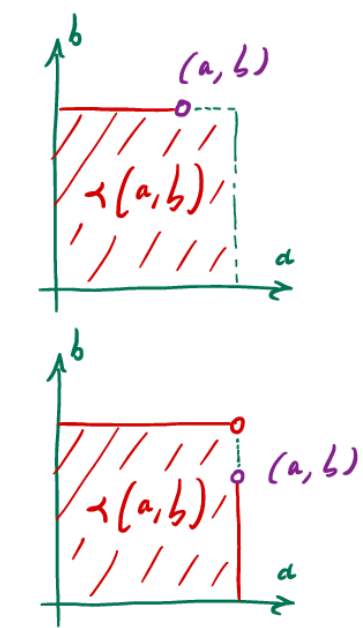
\includegraphics[width=2.5cm]{immagini/ordine_omega.png}
	\end{wrapfigure}
	Che è lo stesso ordinamento che abbiamo usato per dimostrare che il prodotto di numerabili è numerabile.
	\textcolor{MidnightBlue}{In pratica, per confrontare $(a,b)$ con $(a',b')$, si confrontano prima $\max(a,b)$ e $\max(a',b')$;
	a parità si confrontano $a$ e $a'$; se anche queste coincidono, si confrontano $b$ e $b'$.}\\
	Abbiamo già verificato, nella dimostrazione di $\aleph_0^2 = \aleph_0$, che $\prec$ è un buon ordine (con $\omega$ al posto di $\omega_\alpha$, ma le verifiche sono identiche\footnote{Tranne nel caso del buon ordinamento in cui bisogna fare un'induzione transfinita su $\alpha$ per coprire il caso di intersezione non vuota.}).
	Resta da verificare che vale proprio:
	\[ X \Mydef (\omega_\alpha \times \omega_\alpha, \prec) \sim \omega_\alpha
		\]
	Sia $\beta$ l'ordinale corrispondente a $X$, dobbiamo mostrare, per avere l'isomorfismo di buoni ordinamenti, che i cardinali sono uguali, ovvero $\beta = \omega_\alpha$. Siccome $|\omega_\alpha| \leq |\omega_\alpha \cdot \omega_\alpha| = |\beta|$, e $\omega_\alpha$ è iniziale, per la contronominale della definizione di ordinali
	iniziale otteniamo che $\beta \geq \omega_\alpha$, dunque non dobbiamo far altro che escludere che $\omega_\alpha < \beta$, ovvero che $\omega_\alpha$ non è isomorfo ad un segmento iniziale proprio di $X$.\\
	Fissiamo un segmento iniziale proprio $X_{(a,b)}$ di $X$ e dimostriamo che $|X_{(a,b)}| < \aleph_\alpha$, cioè si avrebbe che $|X_{(a,b)}| < |\omega_\alpha|$ e quindi non può accadere che $X_{(a,b)} \sim \omega_\alpha$.\\
	Sia $\mu := \max(a,b)$, essendo $a,b \in \omega_\alpha$, si ha naturalmente che $\mu < \omega_\alpha$ e $\omega_\alpha$ è iniziale, quindi limite, si ha $s(\mu) < \omega_{\alpha}$, e di nuovo $|s(\mu)| < \aleph_\alpha$. Di conseguenza, per la monotonia della funzione degli aleph, $|s(\mu)| = \aleph_\gamma$, per qualche $\gamma < \alpha$, oppure $s(\mu) \in \omega$.
	\begin{itemize}
		\item Nel primo caso $|s(\mu) \times s(\mu)| = \aleph_\gamma^2 \overset{\text{\textcolor{orange}{Hp. indutt.}}}{=} \aleph_\gamma$.
		\item Nel secondo caso $s(\mu) \times s(\mu)$ è finito, e quindi $|s(\mu) \times s(\mu)| < \aleph_0$.
	\end{itemize}
	In ogni caso $|s(\mu) \times s(\mu)| < \aleph_\alpha$ e, siccome vale che $X_{(a,b)} \subseteq s(\mu) \times s(\mu)$, abbiamo allora $|X_{(a,b)}| \leq |s(\mu) \times s(\mu)| < \aleph_\alpha$, come voluto. \hfill $\square$

\begin{exercise}
	Per $n \in \omega$ sia $\ps^n(X) \Mydef \{Y \in \ps(X) : |Y| = n\}$, dimostrare che $\forall n \in \omega$ si ha che $|\ps^n(\omega_\alpha)| = \aleph_\alpha$.
\end{exercise}

\begin{soln}
	Possiamo definire la seguente mappa:
	\[ \omega_\alpha \hookrightarrow \ps^n(\omega_\alpha) : x \mapsto \Imm(f_x)
		\]
	dove:
	\[ f_x : n \to \omega_\alpha : i \mapsto f_x(i) = \begin{cases}
		x &\text{se $i = 0$} \\
		x + i &\text{se $1 \leq i \leq n - 1$}
	\end{cases}
		\]
	Osserviamo in primis che $f_x$ è iniettiva per ogni $x \in \omega_\alpha$, dunque $n = |\Imm(f_x)| \in \ps^n(\omega_\alpha)$, e quindi la mappa sopra è ben definita, infatti $f_x(i) = f_x(j) \to x + i = x + j$,
	e per la stretta monotonia nella seconda componente della somma ordinale si ha $i = j$. Da quanto appena detto segue anche che le funzioni $f_x$ sono strettamente crescenti,
	dunque se $\Imm(f_x) = \Imm(f_y)$, poiché sono insiemi finiti, per cui bene ordinati, ed isomorfi a $n$, l'isomorfismo possibile è uno solo, per un fatto noto, ed è quello definito ricorsivamente che manda ogni volta un elemento 
	nel minimo elemento dell'insieme d'arrivo più grande di tutti quelli dell'immagine ristretta, per cui si ha proprio $f_x = f_y$, da cui $x = f_x(0) = f_y(0) = y$. Abbiamo quindi ottenuto che $\aleph_\alpha = |\omega_\alpha| \leq |\ps^n(\omega_\alpha)|$.\\
	Viceversa, possiamo definire la mappa:
	\[ \ps^n(\omega_\alpha) \to \omega_\alpha^n : A \mapsto (a_0,\ldots,a_{n-1})
		\]
	con $a_i$, $i$-esimo elemento di $A$, ordinato secondo l'ordine di $\omega_\alpha$ ristretto ad $A$. Naturalmente tale mappa è ben definita, visto che ogni insieme produce esattamente una $n$-upla, ed è iniettiva in quanto due $n$-uple uguali implicano tutti
	gli elementi uguali e quindi gli insiemi uguali.\footnote{Questa stessa idea, leggermente modificata per risolvere il problema nel caso $\ps^{\leq n}(\omega_\alpha)$.}
\end{soln}

\begin{exercise}
	Dimostrare che $\psf(\omega_\alpha) = \aleph_\alpha$.\footnote{\textbf{\underline{Hint}}: Osservare che $|$sottoinsiemi finiti di $\omega_\alpha| \leq |\{f : n \to \omega_\alpha | n \in \omega\}|$ [\textcolor{red}{Typo Mamino}], fissare $g : \omega_\alpha \times (\omega_\alpha \sqcup \{\spadesuit\}) \to \omega_\alpha \sqcup \{\spadesuit\}$ biunivoca e definire
	$h : \{f : n \to \omega_\alpha | n \in \omega\} \to \omega_\alpha$ con $h(\emptyset) = \spadesuit$ e $h(f) = g(f(0),h(x \mapsto f(x+1)))$.}
\end{exercise}

\begin{soln}
	Dal basso naturalmente abbiamo la mappa $\omega_\alpha \hookrightarrow \psf(\omega_\alpha) : x \mapsto \{x\}$, che ci dà $\aleph_\alpha \leq |\psf(\omega_\alpha)|$. Per la disuguaglianza opposta, in primis definiamo la mappa:
	\[ \psf(\omega_\alpha) \to \{f \in {}^n \omega_\alpha | n \in \omega\} = \bigcup_{n \in \omega} {}^n\omega_\alpha : A \mapsto f_A
		\]
	dove:
	\[ f_A : m = |A| \to \omega_\alpha : x \mapsto \min\{y \in \omega_\alpha | x \in  A \land y > f_A[x]\}
		\]
	ed osserviamo che poiché le $f_A$ sono strettamente crescenti (in particolare $|A| \in \omega$ ed $A \subseteq \omega_\alpha$ sono bene ordinati, dunque c'è un unico isomorfismo tra loro, ed è quello in cui mappiamo $A$),
	allora $f_A = f_B \implies \Imm(f_A) = \Imm(f_B) \implies A = B$, dunque la mappa è iniettiva ed abbiamo la disuguaglianza $|\psf(\omega_\alpha)| \leq |\{f \in {}^n \omega_\alpha | n \in \omega\}|$. Osserviamo ora che, fissata una
	bigezione $g : \omega_\alpha \times (\omega_\alpha \sqcup \{\spadesuit\}) \to \omega_\alpha \sqcup \{\spadesuit\}$, possiamo definire la mappa:
	\[ h : \{f \in {}^n \omega_\alpha | n \in \omega\} \to \omega_\alpha \cup \{\spadesuit\} : f \mapsto \begin{cases}
		\spadesuit &\text{se $f = \emptyset$} \\
		g(f(0),h(f(x + 1))) &\text{altrimenti}
	\end{cases}
		\]
	che è naturalmente ben definita (grazie a $g$) ed iniettiva, infatti, se abbiamo che $h(f) = h(f')$ in arrivo, o $f = f' = \emptyset$ oppure $g(f(0),f(x+1)) = g(f'(0),f'(x+1))$, che, per la bigettività di $g$, implica $f(0) = f'(0)$ e $h(f(x+1)) = h(f'(x+1))$, che, ripetendo il ragionamento,
	implica a sua volta $f(1) = f'(1)$, e $h(f(x+2)) = h(f'(x+2))$, e così via, ottenendo $f(i) = f'(i)$, $\forall 0 \leq i \leq n-1$, da cui $f = f'$ ed abbiamo l'iniettività. Abbiamo quindi ottenuto che $|\psf(\omega_\alpha)| \leq |\omega_\alpha \sqcup \{\spadesuit\}| = \aleph_\alpha + 1 = \aleph_\alpha$\footnote{L'ultima
	uguaglianza è vera senza AC e la si può ottenere sfruttando disuguaglianze oppure il fatto che $\omega \hookrightarrow \omega_\alpha$.}.
\end{soln}

\begin{exercise}
	Dimostrare che $\forall \alpha,\beta \in \Ord$ si ha:
	\[ |\alpha| = |\beta| = \aleph_\gamma \to |\alpha + \beta| = |\alpha \cdot \beta| = |\alpha^{\beta}| = \aleph_\gamma 
		\]
	dove intendiamo la cardinalità delle tre operazioni ordinali.
\end{exercise}

\begin{soln}
	Per la monotonia [debole] delle operazioni ordinali nella prima componente si ha $\alpha \leq \alpha + \beta, \alpha \cdot \beta, \alpha^\beta$, da cui si ottiene la disuguaglianza dal basso 
	in tutti e tre i casi, $\aleph_\gamma = |\alpha| \leq |\alpha + \beta|, |\alpha \cdot \beta|, |\alpha^\beta|$. Per il viceversa, vediamo caso per caso:
	\begin{itemize}
		\item $\alpha + \beta = \alpha \sqcup \beta$, per cui $|\alpha + \beta| = |\alpha \sqcup \beta| = |\alpha| + |\beta| = \aleph_\gamma + \aleph_\gamma = \aleph_\gamma$.
		\item $\alpha \cdot \beta = \alpha \times \beta$, per cui $|\alpha \cdot \beta| = |\alpha \times \beta| = |\alpha| \cdot |\beta| = \aleph_\gamma \cdot \aleph_\gamma = \aleph_\gamma$.
		\item $\alpha^\beta = \{f \in {}^\alpha\beta : \; |\supp(f)| < \aleph_0\} \subseteq \psf(\alpha \times \beta)$, per cui $|\alpha^\beta| \leq |\psf(\alpha \times \beta)| = |\psf(\omega_\gamma \times \omega_\gamma)| = |\psf(\omega_\alpha)| = \aleph_\gamma$,
		dove l'uguaglianza tra la cardinalità dele parti finite è indotta dalla bigezione tra gli insiemi (basta fissare una bigezione e poi definire quella tra gli insiemi mandando ogni elemento delle prime parti finite nella sua immagine tramite la prima bigezione),
		mentre l'ultima uguaglianza è l'esercizio precedente.
	\end{itemize}
\end{soln}

\begin{exercise}
	Se $|X| = \aleph_\alpha$ e $f : X \to Y$ è una funzione, allora $|f[X]| \leq \aleph_\alpha$.
\end{exercise}

\begin{soln}
	Possiamo assumere, a meno di bigezione, che $X = \omega_\alpha$ e definire la funzione:
	\[ g : f[X] \to X : y \mapsto \min_<(f^{-1}(y))
		\]
	che è naturalmente ben definita ed è iniettiva perché stiamo considerando i minimi di una partizione di $X$, dunque due minimi sono uguali se e solo se consideriamo lo stesso elemento della partizione di $X$, cioè la stessa controimmagine,
	da cui si ottiene, applicando $f$, che in partenza i valori devono essere uguali.
\end{soln}

\begin{exercise}
	Dimostrare che $\forall \alpha \; \in \Ord \; \aleph_{\alpha + 1} < 2^{2^{\aleph_\alpha}}$.
\end{exercise}

\begin{soln}
	Poiché per Cantor si ha $\aleph_\alpha < 2^{\aleph_\alpha}$, essendo per definizione ricorsiva della funzione degli aleph, che $\aleph_{\alpha + 1}$ è il più piccolo ordinale iniziale infinito strettamente maggiore di $\aleph_\alpha$, si ha $\aleph_{\alpha + 1} \leq 2^{\aleph_\alpha}$.
	Infine si osserva che $\aleph_{\alpha} \leq 2^{\aleph_\alpha} < 2^{2^{\aleph_\alpha}} \to \aleph_{\alpha} < 2^{2^{\aleph_\alpha}}$.
\end{soln}
\section{L'assioma della scelta}
L'assioma della scelta è stato introdotto da \href{https://en.wikipedia.org/wiki/Ernst_Zermelo}{\textcolor{purple}{Ernst Zermelo}} nel 1904, per dimostrare che ogni insieme è ben ordinabile.
Si potrebbe dubitare del valore di una dimostrazione ottenuta introducendo un assioma ad hoc, è tuttavia opportuno osservare che l'assioma della scelta è stato usato prima di Zermelo, ma senza accorgersene.
Quindi Zermelo non ha tanto costruito un nuovo principio, quanto piuttosto riconosciuto la necessità di codificare un principio già applicato, ma in modo impreciso.
Inoltre, gli assiomi che abbiamo introdotto fin'ora non permettono, per esempio, né di affermare né di negare la buona ordinabilità di $\RR$. Quindi, se si vuole dare una risposta al problema dell'esistenza di un buon ordine 
di $\RR$, che sia positiva o negativa, questa deve per forza venire da un nuovo assioma. In questo senso, Zermelo dice che il teorema del buon ordinamento è ragionevole perché segue da una ipotesi - l'assioma della scelta - ragionevole.
Anzi, così ragionevole che i matematici l'hanno usato senza neppure accorgersi che questo assioma è effettivamente un'ipotesi.

\begin{axiom}[Assioma della scelta (AC)]
	\label{ax9}
	Dato un insieme $X$ di insiemi non vuoti, esiste una \vocab{funzione di scelta} $f : X \rightarrow \bigcup X$ tale che $\forall a \in X \; f(a) \in a$\footnote{Cioè la funzione manda ogni elemento $a$ di $X$ in un suo elemento.}.
	In simboli:
	\[ \forall X (\emptyset \not \in X) \rightarrow (\exists f \in {}^X\left(\bigcup X\right) \; \forall a \in X \; f(a) \in a)\footnote{Letteralmente le funzioni di scelta ``scelgono'' un elemento in cui mandare tutto l'insieme, preso a sua volta come elemento.}
		\]
\end{axiom}

L'assioma della scelta è, di frequente, applicato per \vocab{fissare infiniti elementi}. Per esempio, dovendo costruire una successione $x_n$ che tende a $+\infty$, capita di ragionare dicendo
\textcolor{MidnightBlue}{per ogni $n \in \NN$ fisso $x_n > n$ che abbia questa o quella proprietà che mi interessano.}\\
Formalmente, in questo ragionamento, stiamo dicendo \textcolor{MidnightBlue}{considero}:
\[ X = \{ \rbrack n,+\infty\rbrack | n \in \NN\}
	\]
\textcolor{MidnightBlue}{e considero} $f : X \rightarrow \bigcup X \subseteq \RR$ \textcolor{MidnightBlue}{una funzione di scelta per $X$. Ora pongo $x_n = f(]n,+\infty])$}. Si pone quindi una domanda: perché non ci serve alcun assioma per fissare un elemento - come a dire \textcolor{MidnightBlue}{considero un
numero $\varepsilon$ tale che etc.} - ma ci serve per fissarne infiniti?\\

Il principio che, sapendo che ci sono oggetti che godono di una certa proprietà, ci permette di fissarne uno, è una legge logica.\\
Questa legge, da un lato, è valida in ogni \vocab{teoria del primo ordine}, non solo nella teoria degli insiemi. D'altro canto, può essere vista come una mera scorciatoia nei ragionamenti, perché se da $\exists x \; \varphi(x)$ possiamo dedurre una $\psi$ che non menziona $x$,
fissando un $x$ che soddisfa $\varphi(x)$, allora si può dimostrare che, a patto di presentare il ragionamento nella maniera opportuna, la conclusione $\psi$ può essere raggiunta senza bisogno di fissare $x$\footnote{Cioè se fissando $x$ il predicato diventa una proposizione vera, con cui continuare il ragionamento, si dimostra che si può arrivare a $\psi$ anche senza 
bisogno di fissare $x$, in questo senso è come se l'azione di ``fissare'' un elemento fosse un'azione vuota, nel senso che il ragionamento formalmente può essere portato avanti anche senza richiederla, ma noi lo facciamo perché ci è comodo ragionare così, ma si può equivalentemente procedere senza effettivamente farlo.}. In questo senso, la possibilità
di fissare un oggetto - cioè dare un nome ad un oggetto - è una legge del pensiero: una caratteristica del modo in cui ragioniamo.\\
Tecnicamente, questa legge è vendicata [nel senso di rivendicata] dal \vocab{teorema di completezza di Gödel}, che dice che la logica del primo ordine è quella giusta per catturare una nozione molto naturale di \vocab{modello}.\\
L'assioma della scelta, d'altra parte, \textcolor{red}{si può vedere} come un modo per fissare elementi, ma \textcolor{red}{si concretizza} in un enunciato insiemistico, che asserisce l'esistenza di un certo insieme: la funzione di scelta.
Non si tratta dunque di una caratteristica del nostro modo di ragionare - di una legge del pensiero - perché nulla ci obbliga a pensare in termini insiemistici, e, d'altro canto, nulla obbliga gli insiemi a fare quello che il nostro intuito ci dice dovrebbero fare.
Insomma, questo è l'intoppo: che non sappiamo esprimere il concetto di \textcolor{MidnightBlue}{fissare infinite variabili} se non tramite l'espediente di \textcolor{MidnightBlue}{fissare una singola funzione di scelta}\footnote{Che fissi in un solo colpo tutti gli infiniti elementi.}. Tuttavia, per fare questo dobbiamo asserire l'esistenza di un certo insieme, appunto la funzione di scelta,
che, si può dimostrare, non segue dagli assiomi 1-8. Bando alle ciance.

\begin{note}[Ogni funzione surgettiva ha inversa destra]
	AC equivale all'affermazione che ogni funzione surgettiva ha un inversa destra, ossia:
	\[ \forall f : X \rightarrow Y \; \text{surgettiva}\;\exists g : Y \rightarrow X \; f \circ g = \id_Y
		\]
\end{note}

\begin{proof}
	Verifichiamo che l'enunciato sopra è un fatto equivalente ad AC.
	\begin{itemize}
		\item[$\boxed{\Longrightarrow}$] Consideriamo l'insieme delle controimmagini via $f$ degli elementi di $Y$:
		\[ Z \Mydef \{A \in \ps(X) | \exists y \in Y \; \overbrace{\forall x \in X \; x \in A \leftrightarrow f(x) = y}^{A = f^{-1}(y)}\}
			\]
		Per la surgettività di $f$ gli elementi di $Z$ sono tutti non vuoti, dunque per \hyperref[ax9]{AC} esiste $h : Z \rightarrow \bigcup Z = X$ funzione di scelta.
		Definiamo quindi $g(y) \Mydef h(f^{-1}(y))$ - più precisamente $g(y) = h(\{x \in X | f(x)  = y\})$, segue che:
		\[ f \circ g(y) = f(g(y)) = f(h(\{x \in X | f(x)  = y\}))
			\]
		ed essendo $h$ una funzione di scelta, si ha che $h(A) \in A$, dunque $h(f^{-1}(y)) \in f^{-1}(y)$, quindi fa un certo elemento nella controimmagine di $y$, fissato dalla nostra funzione di scelta $h$, e, indipendentemente da quale sia, torniamo indietro con $f$, dunque:
		\[ f(z) = y \qquad \text{con $z \in f^{-1}(y)$}
			\]
		\item[$\boxed{\Longleftarrow}$] Verifichiamo ora che da questo fatto derivi l'assioma della scelta. Sia $X$ un insieme di insiemi non vuoti, consideriamo l'insieme $X' = \{(a,A) \in \left(\bigcup X\right) \times X | a \in A \land A \in X\}$.
		La funzione:
		\[ f : X' \rightarrow X : (a,A) \mapsto A
			\]
		è banalmente surgettiva, quindi per ipotesi ha un'inversa destra $g : X \hookrightarrow X'$ che manda $A$ in una coppia $(a,A)$ per qualche $a \in A$\footnote{Che fissa $a \in A$ senza scriverlo esplicitamente.}.
		Ora quindi la funzione:
		\[ h : X \rightarrow \bigcup X : A \mapsto \text{prima componente di $g(A)$}
			\]
		è una funzione di scelta per $X$, perché prendiamo la prima componente di $g(A)$, che sta in $A$, e questa è determinata da $g$, cioè $h(A) \in A$.
	\end{itemize}
\end{proof}

L'assioma della scelta forma, insieme ai due enunciati seguenti - il teorema del buon ordinamento ed il lemma di Zorn - una terna classica di proposizioni equivale, nel senso che gli assiomi 1-8, unitamente ad una qualunque delle tre proposizioni, implicano le altre due.

\begin{theorem}[Teorema del buon ordinamento - o di Zermelo]
	\label{buon_ordinamento}
	Ogni insieme è ben ordinabile, ovvero:
	\[ \forall S \; \exists < \in S \times S \; (S,<)\;\text{è un buon ordinamento}
		\]
\end{theorem}

\begin{definition}[Sottocatena - maggiorante - massimale]
	Dato $(S,<)$ un ordine parziale abbiamo che:
	\begin{itemize}
		\item una \vocab{sottocatena} è un $A \subseteq S$ tale che $(A,<_{|A})$, cioè $A$ con la restrizione dell'ordine di $S$ ad $A$, è un ordine totale
		\item un \vocab{maggiorante} di $A \subseteq S$ è un $x \in S$ tale che $\forall y \in A \; y \leq x$
		\item $x \in S$ è un elemento \vocab{massimale} se $\neg \exists y \in S \; x < y$.
	\end{itemize}
\end{definition}

\begin{lemma}[Lemma di Zorn]
	\label{Zorn}
	Ogni insieme parzialmente ordinato, in cui ogni sottocatena ammette un maggiorante ha elementi massimali.
\end{lemma}

\begin{theorem}[AC $\iff$ buon ordinamento $\iff$ Zorn]
	Le tre affermazioni \hyperref[ax9]{assioma della scelta}, \hyperref[buon_ordinamento]{teorema del buon ordinamento} e \hyperref[Zorn]{lemma di Zorn} sono equivalenti -
	ossia si implicano vicendevolmente assumendo gli assiomi 1-8.
\end{theorem}

\subsection{\texorpdfstring{Buon ordinamento $\rightarrow$ AC}{Buon ordinamento implica AC}}

\begin{proof}
	(Buon ordinamento $\rightarrow$ AC)\\
	Dato $S$ insieme di insiemi non vuoti, fissiamo, per il \hyperref[buon_ordinamento]{teorema del buon ordinamento}, un buon ordine $\prec$ su $\bigcup S$. Allora la funzione:
	\[ f : S \rightarrow \bigcup S : x \mapsto \min_{\prec}(x)
		\]
	è una funzione di scelta per $S$ [perché naturalmente $\min_\prec (x) \in x$, e il fatto che per Zermelo sappiamo che $\prec$ è un buon ordinamento su $S$, ma non sappiamo esplicitamente cosa faccia, ci dice che, tale funzione fissa il minimo, ma non sappiamo necessariamente chi sia, perché non 
	conosciamo esplicitamente $\prec$, da cui la funzione di scelta].
\end{proof}

\subsection{\texorpdfstring{AC $\rightarrow$ buon ordinamento (idea)}{AC implica buon ordinamento (idea)}}
\textcolor{MidnightBlue}{Dimostreremo questo risultato tramite la catena di deduzioni AC $\rightarrow$ Zorn $\rightarrow$ buon ordinamento. Tuttavia conviene studiare l'idea di una dimostrazione diretta.}

\begin{proof}
	(AC $\rightarrow$ buon ordinamento (idea))\\
	Fissiamo un insieme $X$, per \hyperref[ax9]{AC}, esiste una funzione di scelta:
	\[ f : \ps(X) \setminus\{\emptyset\} \rightarrow \bigcup \ps(X) = X : A \mapsto f(A) \in A
		\]
	Ora vorremmo mettere in ordine gli elementi di $X$ come segue;
	\[ F(0) = x_0 = f(X) \qquad F(1) = x_1 = f(X \setminus \{x_0\}) \qquad F(2) = x_2 = f(X \setminus \{x_0,x_1\}) \qquad\ldots
		\]
	ogni volta scegliendo un elemento nuovo fra quelli che rimangono ancora da elencare. Chiaramente non è detto che questo procedimento termini
	in una quantità numerabile di passi, per cui potremmo dover definire $x_\omega = f(X\setminus\{x_0,x_1,x_2,\ldots\})$ e, più in generale, possiamo definire per ricorsione transfinita:
	\[ F(\alpha) = f(X \setminus\{x_\beta | \beta < \alpha\}) = f(X \setminus F[\alpha])
		\]
	Questa cosa non può funzionare per tutti gli ordinali, cioè $F$ non è ben definita, perché da un certo punto in poi $F[\alpha] = X$ e non possiamo usare la funzione di scelta sul vuoto, se per assurdo $F[\alpha] \subsetneq X$ per ogni $\alpha \in \Ord$, allora staremmo immergendo la classe degli ordinali in un insieme, tramite $\alpha \mapsto F(\alpha) \in X$,
	che è ancora assurdo (si avrebbe che l'Hartogs $H(X)$ si immerge in $X$ ad un certo punto o anche è violato Burali-Forti).\\
	Per rimediare a questo inconveniente definiamo quindi
	\[ F(\alpha) = \begin{cases}
		f(X \setminus F[\alpha]) &\text{se $F[\alpha] \subsetneq X$} \\
		\spadesuit &\text{altrimenti}
	\end{cases}
		\] 
	che ora è una funzione classe $\Ord \to X \cup \{\spadesuit\}$ ben definita. A questo punto consideriamo $\beta := \min\{\gamma : F(\gamma) = \spadesuit\}$, che è ben definito poiché è un insieme di ordinali, non vuoto in 
	quanto se fosse vuoto ricadremmo in uno dei due assurdi citati sopra, pertanto si ha che $F[\beta] = X$ e $F_{|\beta}$ è una mappa iniettiva in quanto $f$ è iniettiva per definizione, per cui $X$ è in bigezione con l'ordinale $\beta$
	e quindi può essere ben ordinato mediante un ordinamento indotto, per cui abbiamo ottenuto Zermelo.
\end{proof}

\subsection{\texorpdfstring{Zorn $\rightarrow$ buon ordinamento}{Zorn implica buon ordinamento}}

\begin{proof}
	(Zorn $\rightarrow$ buon ordinamento)\\
	Vogliamo dimostrare che un insieme $S$ è ben ordinabile. Consideriamo:
	\[ \begin{split}
		T &:= \{f : \alpha \to S | \;\text{$\alpha < H(S)$ e $f$ iniettiva}\} \textcolor{MidnightBlue}{=\{\text{funzioni iniettive da un ordinale a $S$}\}} \\
		  &= \{f \in \ps(H(S) \times S) | \; \text{$f$ è una funzione iniettiva e $\Dom(f) \in \Ord$}\}
	\end{split}
		\]
	\footnote{Deve essere necessariamente che $\alpha < H(S)$, perché se $\alpha \geq H(S)$ si immergesse in $S$, allora una restrizione dell'immersione permetterebbe di immergere anche $H(S)$ in $S$, che è assurdo, dunque 
	gli ordinali che si possono immergere in $S$ sono soltanto quelli più piccoli del suo Hartogs. Si noti inoltre che $T$ è non vuoto perché c'è sempre la funzione da 0 a $S$ o da 1 ad $S$, se $S$ è non vuoto.}Osserviamo
	che $T$ è parzialmente ordinato dalla relazione d'ordine $f < g \equiv f \subseteq g$. Diamo per buono che $(T,<)$ soddisfa le ipotesi del 
	lemma di Zorn, e quindi esiste $f \in T$ massimale rispetto alla relazione $<$. Abbiamo che $f$ è surgettiva, infatti, se non lo fosse $S \setminus \Imm(f) \ne \emptyset$, dunque esiste $y \in S \setminus \Imm(f)$ e possiamo definire:
	\[ f' = f \cup \{(\Dom(f),y)\}
		\]
	dove $\Dom(f)$ è l'ordinale successore al massimo del dominio di $f$, ed $f'$ è iniettiva perché unione di funzione iniettive su insiemi in arrivo disgiunti, quindi avremmo $f' > f$ e $f \in T$, che va contro la massimalità di $f$, quindi è assurdo.
	Abbiamo quindi che $S$ è in bigezione con $\Dom(f) \in \Ord$, dunque è bene ordinabile, perché possiamo indurre un buon ordinamento su $S$ via $f$, e quindi abbiamo il teorema del buon ordinamento.\\
	\textcolor{purple}{Verifica delle ipotesi del del lemma di Zorn}\\
	Dobbiamo verificare che data $P \subseteq T$ una sottocatena di $T$, ha sempre un maggiorante, verifichiamo che $f := \bigcup P$ è il maggiorante in questione. In primis osserviamo che $f$ è una funzione ben definita, infatti, essendo un'unione di funzioni
	ci basta verificare, per un'osservazione vista in precedenza, che per ogni $g_1,g_2 \in P$ se $x \in \Dom(g_1) \cap \Dom(g_2)$, allora $g_1(x) = g_2(x)$ (in tal modo $f$ è effettivamente una funzione), essendo che $(P,<_{|P})$ è totalmente ordinato, allora vale WLOG $g_1 > g_2$,
	ovvero $g_2 \subseteq g_1$, dunque le due funzioni coincidono su $x$, perché una estende l'altra.\\
	Verifichiamo ora che $f$ è iniettiva, se $f(x) = f(y)$, allora esistono, per definizione di unione, $g_1,g_2 \in P$ tali che $g_1(x) = f(x)$ e $g_2(y) = f(y)$, ma, come prima, essendo $P$ totalmente ordinato, vale WLOG $g_1 \supseteq g_2$, per cui $g_1(x) = g_2(y) = g_1(y)$, ed essendo $g_1 \in T$ è iniettiva, dunque si conclude $x = y$.
	Osserviamo inoltre che, per le proprietà degli ordinali:
	\[ \Dom(f) = \bigcup\{\Dom(g) | g \in P\} = \sup\{\Dom(g) | g \in P\}
		\]
	dove il sup è un ordinale per quanto visto sugli insiemi di ordinali. A questo punto $f$ è ben definita, ha dominio un ordinale ed è iniettiva, per cui $f \in T$. Ci resta da verificare che $f$ sia un maggiorante per $P$, ma ciò è banale per come abbiamo costruito $f$, infatti:
	\[ \forall g \in P \; g \subseteq \bigcup P = f \equiv g \leq f
		\]
\end{proof}
 
\subsection{\texorpdfstring{AC $\rightarrow$ Zorn}{AC implica Zorn}}

\begin{proof}
	(AC $\rightarrow$ Zorn)\\
	Sia $(S,<)$ un insieme parzialmente ordinato. Supponiamo che ogni sottocatena di $S$ abbia un maggiorante e che, per assurdo, $S$ non abbia elementi massimali.
	Questa assunzione si traduce nel fatto che ogni elemento di $S$ ammette un maggiorante stretto in $S$, $\forall x \in S \; \exists y \in S \; y > x$ (è la negazione della definizione di esistenza di un elemento massimale), ora per ipotesi ogni sottocatena $A$ ammette un maggiorante in $S$, che può essere a sua volta maggiorato strettamente per quanto appena detto,
	dunque ogni sottocatena ammette un maggiorante stretto - d'altronde se ci fosse una sottocatena con un maggiorante non stretto, che quindi non può essere maggiorato strettamente da nessun altro elemento di $S$, allora sarebbe un elemento massimale per quest'ultimo, contraddicendo la nostra ipotesi.\\
	Sia $f : \ps(S) \setminus \{\emptyset\} \to \bigcup \ps(S) \setminus \{\emptyset\} = S$ una funzione di scelta per i sottoinsiemi di $S$. L'idea è ora di costruire per induzione transfinita una funzione classe crescente [quindi iniettiva] $F : \Ord \to S$ - che chiaramente non può esistere 
	perché altrimenti $F_{|H(S)}$ sarebbe un'immersione di $H(S)$ in $S$, e dunque avremmo l'assurdo (alternativamente anche perché violeremmo Burali-Forti). Vorremmo costruire $F$ tramite la ricorsione transfinita forte come segue:
	\[ F(\alpha) = f(\{\text{maggioranti stretti di $F[\alpha]$}\})
		\]
	perché questa costruzione abbia senso, è necessario che $F_{|\alpha}$ sia [debolmente] crescente, un questo modo $F[\alpha]$ è una sottocatena di $S$ e, per l'osservazione sopra, l'insieme dei maggioranti stretti non è vuoto, ed ha senso applicare ad esso la funzione di scelta $f$, e dunque la $F$ è ben definita,
	inoltre è strettamente crescente per costruzione.\\
	Per assurdo consideriamo il minimo (possiamo farlo per l'ipotesi assurda e per i soliti motivi sugli insiemi di ordinali) $\alpha$ tale che $F_{|\alpha}$ non è [debolmente] crescente. Quindi esistono $\gamma < \delta < \alpha$ tali che $F(\gamma) \not \leq F(\delta)$ ($S$ non è detto sia un ordine totale,
	quindi non possiamo dire che $F(\gamma) > F(\delta)$). Però siccome $\delta < \alpha$, per la minimalità di quest'ultimo, $F_{|\delta}$ è crescente, per cui $F(\delta)$ è ben definita
	ed è un maggiorante stretto di $F[\delta]$, quindi, in particolare, $F(\gamma) < F(\delta) \; \lightning$.\\
	\textcolor{red}{\underline{Questo modo di procedere, però, contiene un'imprecisione formale}}\\
	Per applicare il teorema di ricorsione transfinita alla costruzione di $F$ dobbiamo scrivere $F(\alpha) = G(F_{|\alpha})$. La $G$ della costruzione precedente è:
	\[ G(h) = f(\{\text{maggioranti stretti dell'immagine di $h$}\})
		\]
	Questa però non è una funzione classe definita da $V$ a $V$ (in arrivo può essere qualsiasi cosa), come richiesto dal teorema di ricorsione transfinita, perché non è definita se l'immagine di $h$ non ha maggioranti stretti in $S$. Il ragionamento si aggiusta così: si fissa $\spadesuit \not \in S$ e si definisce:
	\[ F(\alpha) = \begin{cases}
		f(\{\text{maggioranti stretti di $F[\alpha]$}\}) &\text{se $F_{|\alpha} : \alpha \to S$ è crescente} \\
		\spadesuit &\text{altrimenti}
	\end{cases}
		\] 
	ora tutti i casi sono coperti ed è lecito applicare il teorema di ricorsione transfinita. Se $F$ non fosse una funziona classe crescente $\Ord \to S$, ci sarebbe il minimo $\alpha$ tale che $F_{|\alpha}$ non è
	$\alpha \to S$ crescente, e, ragionando come prima si ottiene un assurdo.\\
	Ricapitolando, negando la tesi, abbiamo costruito una funzione classe crescente, dunque iniettiva $\Ord \to S$, che non può esistere per il teorema di Hartogs.
\end{proof}

\begin{remark}
	Il problema sottile che si presenta sopra è che nell'enunciato del teorema di ricorsione transfinita la $G$ richiesta deve essere ben definita su tutto $V$, e, prima della correzione (in particolare abbiamo dovuto aggiungere un valore per l'immagine 
	per tutti gli insiemi che non sono ordinali) nel caso sopra, non lo era.
\end{remark}

\pagebreak
\subsection{Conseguenze immediate di AC}

\begin{proposition}[Tutti le cardinalità infinite sono aleph]
	Ogni insieme è equipotente ad un ordinale iniziale\footnote{Per gli insiemi finiti lo sapevamo già, senza bisogno di AC.}. In particolare, ogni cardinalità infinita è un aleph.
\end{proposition}

\begin{proof}
	Per il \hyperref[buon_ordinamento]{teorema del buon ordinamento} ogni insieme è bene ordinabile, quindi isomorfo ad un ordinale, e per le proprietà
	degli ordinali iniziali (cioè sono i rappresentati di tutte le cardinalità \textcolor{purple}{di ordinali}), ogni insieme è equipotente ad un ordinale iniziale.
	La seconda affermazione segue dal fatto che gli $\omega_\alpha$ sono tutti e soli gli ordinali iniziali infiniti, per quanto detto, dunque tutte le cardinalità infinite, prima di ordinali ed ora,
	con AC, di qualunque insieme, sono aleph.
\end{proof}

\begin{remark}[Tutti gli insiemi sono isomrofi ad un ordinale $\implies$ AC]
	Viceversa, assumere che ogni insieme è equipotente ad un ordinale implica AC.
\end{remark}

\begin{proof}
	Dal fatto che ogni $X$ è equipotente ad un ordinale deduciamo il teorema del buon ordinamento. Se $|X| = |\alpha|$, con $\alpha \in \Ord$, c'è una bigezione tra $X$ ed $\alpha$, e tale bigezione induce un buon ordinamento su $X$.
\end{proof}

\begin{corollary}[L'ordine fra le cardinalità è totale]
	Tutte le cardinalità sono confrontabili, ovvero:
	\[ \forall X,Y \; |X| < |Y| \lor |X| = |Y| \lor |Y| < |X|
		\]
\end{corollary}

\begin{proof}
	Dalla proposizione sopra sappiamo ora che anche tutte le cardinalità infinite sono ordinali, dunque tutte le cardinalità sono ordinali e queste sappiamo già [senza AC] che sono tutte confrontabili.
\end{proof}

\begin{remark}[Cardinalità confrontabili $\implies$ AC]
	La confrontabilità delle cardinalità implica \hyperref[ax9]{AC}.
\end{remark}

\begin{proof}
	Dimostriamo che il \hyperref[buon_ordinamento]{teorema del buon ordinamento} segue dall'ipotesi che tutte le cardinalità siano confrontabili. Consideriamo il confronto fra $|X|$ e $|H(X)|$.
	Per la definizione di $H(X)$ non può valere $|H(X)| \leq |X|$, quindi per ipotesi di confrontabilità totale, deve necessariamente valere che $|X| < |H(X)|$, ovvero esiste $f : X \hookrightarrow H(X) \in \Ord$ iniettiva,
	per cui si ha che $f[X] \subsetneq H(X)$ è un insieme di ordinali, dunque ben ordinato, e ciò induce un buon ordinamento su $X$.
\end{proof}
\pagebreak
\begin{corollary}[AC $\implies |X \times X| = |X|$]
	Per ogni insieme $X$ infinito, vale che $|X \times X| = |X|$.
\end{corollary}

\begin{proof}
	Per quanto visto, tutte le cardinalità infine sono aleph, dunque $|X| = \aleph_\alpha$, per cui:
	\[ |X \times X| = \aleph_\alpha \cdot \aleph_\alpha \overset{(\star)}{=} \aleph_\alpha = |X|
		\]
	dove $(\star)$ è il fatto già visto che per ogni $\alpha \in \Ord \; \aleph_\alpha \cdot \aleph_\alpha = \aleph_\alpha$.
\end{proof}

\begin{note}[Teorema di Tarski]
	Vale anche che $|X \times X| = |X| \implies$ AC, questo è il teorema di Tarski che vedremo più avanti.
\end{note}


\begin{corollary}[$X$ infinito $\leftrightarrow \aleph_0\leq |X|$]
	Ogni insieme infinito ha un sottoinsieme numerabile cioè:
	\[ \forall X \; \text{$X$ infinito $\leftrightarrow \aleph_0 \leq |X|$}
		\]
\end{corollary}

\begin{proof}
	Abbiamo già dimostrato $\leftarrow$ (per l'\hyperref[omega_Dedekind_finito]{osservazione 6.5}, $X$ non è Dedekind-finito, ma, essendo che finito $\implies$ Dedekind-finito [senza bisogno di AC],
	la contronominale ci dice che $X$ non è finito, dunque $X$ infinito), mentre la freccia $\rightarrow$ opposta segue dal fatto che, $X$ infinito implica per AC $|X| = \aleph_\alpha$, per quanto visto,
	ma per la definizione ricorsiva della funzione aleph, $\omega = \omega_0 \leq \omega_\alpha$, $\forall \alpha \in \Ord$, dunque si ha proprio:
	\[ |X| = \aleph_\alpha = |\omega_\alpha| \geq |\omega| = \aleph_0
		\]
\end{proof}

Ricordiamo che un insieme si dice \vocab{Dedekind-finito} (o \vocab{finito secondo Dedekind}) se non può essere messo in corrispondenza biunivoca con un suo sottoinsieme proprio.

\begin{proposition}[Insieme finito $\iff$ Dedekind-finito]
	Osserviamo che vale che $X$ finito $\leftrightarrow X$ è Dedekind-finito.
\end{proposition}

\begin{proof}
	Vediamo le due frecce.
	\begin{itemize}
		\item[$\boxed{\rightarrow}$] Già visto in precedenza, è il \hyperref[cassetti]{principio dei cassetti}.
		\item[$\boxed{\leftarrow}$] Vediamo la contronominale, se $X$ è infinito, allora per la proposizione precedente $\aleph_0 \leq |X|$, ovvero $\omega \hookrightarrow X$\footnote{Come accennato nel capitolo sulle cardinalità finite è proprio il fatto che ci serve per concludere l'equivalenza e ci viene dato appunto da AC.}, allora possiamo definire la mappa:
		\[ g : X \rightarrow X : x \mapsto \begin{cases}
			f \circ s \circ f^{-1} (x) &\text{se $x \in f[\omega]$} \\
			x &\text{altrimenti}
		\end{cases}
			\]
		tale funzione è iniettiva in quanto in tutti in entrambi i casi le funzioni sono iniettive (nel primo caso è una composizione di funzioni iniettive), e si osserva che $f(0) \not \in \Imm(g)$, infatti in questo caso si avrebbe che $f(s(f^{-1}(x))) = f(x) \implies f(s(y)) = f(0) \implies s(y) = 0 \; \lightning$, dunque si ha $|X| = |g[X]|$ e $g[X] \subsetneq X$, per cui $X$ non è Dedekind-finito.\\
		Alternativamente, sempre per dimostrare la contronominale, per AC abbiamo che $X$ infinito implica $|X| = |\omega_\alpha|$ per qualche $\alpha \in \Ord$, dunque esiste una bigezione $f$ tra $X$ e $\omega_\alpha$ e possiamo, in maniera simile a sopra, definire:
		\[ g : X \to X : x \mapsto f \circ s \circ f^{-1}(x)
			\]
		come prima tale mappa è iniettiva e $f(0) \not \in \Imm(g)$, dunque $X$ è in bigezione col sottoinsieme proprio $\Imm(g)$, per cui non è Dedekind-finito.
	\end{itemize}
\end{proof}

\begin{proposition}[Surgettività $\iff$ disuguaglianza tra cardinalità]
	Vale che:
	\[ 0 < |X| \leq |Y| \leftrightarrow \exists f : Y \twoheadrightarrow X \; \text{surgettiva}
		\]
\end{proposition}

\begin{proof}
	Vediamo le due implicazioni.
	\begin{itemize}
		\item[$\boxed{\rightarrow}$] Per ipotesi $|X| \leq |Y|$, cioè esiste $g : X \hookrightarrow Y$ iniettiva, fissato $a \in X$ (stiamo usando che $X$ è non vuoto), possiamo definire:
		\[ f : Y \rightarrow X : y \mapsto \begin{cases}\footnote{Typo di mamino nel primo caso, deve essere $g$ non $f$.}
			g^{-1}(y) &\text{se $y \in g[X]$} \\
			a &\text{altrimenti}
		\end{cases}
			\]
		e tale funzione è banalmente surgettiva.
		\item[$\boxed{\leftarrow}$] Viceversa, data $f : Y \twoheadrightarrow X$ surgettiva, abbiamo visto che è un fatto equivalente ad \hyperref[ax9]{AC} dire che esiste un'inversa destra, $h : X \rightarrow Y$,
		che è iniettiva, per definizione di inversa da $\Imm(f) = X$ a $Y$, e quindi ci dà proprio che $|X| \leq |Y|$.
	\end{itemize}
\end{proof}

\begin{proposition}[Unione di al più $\aleph_\alpha$ insiemi al più $\aleph_\alpha$]
	Se $S$ è un insieme, di cardinalità al più $\aleph_\alpha$, di insiemi, di cardinalità al più $\aleph_\alpha$, allora l'unione di $S$ è a sua volta un insieme di cardinalità al più $\aleph_\alpha$, in simboli:
	\[ |S| \leq \aleph_\alpha \; \forall A \in S \; |A| \leq \aleph_\alpha \rightarrow \left\lvert \bigcup S \right\rvert \leq \aleph_\alpha 
		\]
\end{proposition}

\begin{proof}
	Possiamo assumere $\emptyset \not \in S \ne \emptyset$. Cerchiamo una mappa $f : \omega_\alpha \times \omega_\alpha \to \bigcup S$ surgettiva per avere la disuguaglianza. Per ipotesi possiamo fissare $g : \omega_\alpha \twoheadrightarrow S$ surgettiva,
	inoltre, detto $H_{A} = \{h : \omega_\alpha \twoheadrightarrow A | \; \text{$h$ surgettiva}\}$, sappiamo per ipotesi che per ogni $A \in S \; H_A \ne \emptyset$, dunque possiamo applicare AC all'insieme $\{H_A\}_{A \in S}$ ed ottenere $\iota$ tale che $\iota(H_A) \in H_A$\footnote{Anche se fossimo nel caso di $\aleph_0$ questo passaggio 
	non può essere aggirato, bisogna necessariamente ricorrere ad AC.}. A questo punto è facile definire:
	\[ f : \omega_\alpha \times \omega_\alpha \twoheadrightarrow \bigcup S : (x,y) \mapsto (\iota(H_{g(x)}))(y) \;\footnote{Volendo essere precisissimi, anziché mandare $g(x)$ al pedice di $H$ dovremmo usare due funzioni.}
		\]
	e si osserva che una tale mappa è surgettiva, infatti, preso $z \in \bigcup S$, allora esiste $A \in S$ tale che $z \in A$, dunque per la surgettività di $g$ esiste $x \in \omega_\alpha$ per cui $g(x) = A$; osservando ora che $\iota(H_{g(x)})$ è surgettiva da $\omega_\alpha$ ad $A$ si ha 
	che esiste $y \in \omega_\alpha$ tale che $(\iota(H_{g(x)}))(y) = z$, da cui si conclude.
\end{proof}

\begin{corollary}[Unione al più numerabile di insiemi al più numerabili]
	Un'unione numerabile (o anche al più numerabile) di insiemi numerabili (al più numerabile) è numerabile (al più numerabile).
\end{corollary}

\begin{remark}[Parti di cardinalità al più $n$]
	Sia $\ps^{\leq n}(X) \Mydef \{A \in \ps(X) : |A| \leq n\}$, se $X$ è infinito e $0 < n < \omega$, allora $|\ps^{\leq n}(X)| = |X|$.
\end{remark}

\begin{proof}
	La disuguaglianza $|X| \leq |\ps^{\leq n}(X)|$ si ottiene con la mappa iniettiva che manda ogni elemento nel suo singoletto $X \hookrightarrow \ps^{\leq n}(X) : x \mapsto \{x\}$.\\
	Per dimostrare la disuguaglianza dall'alto possiamo procedere in due modi equivalenti, o definendo la mappa:
	\[ \ps^{\leq n}(X) \supseteq \{A \in \ps(X) : 0 < |A| \leq n\} \hookrightarrow {}^n X : A \mapsto \iota(H_A)
		\]
	con $H_A = \{f : n \twoheadrightarrow A\}$ (che è non vuoto per $A$ nell'insieme in partenza) e $\iota$ funzione di scelta su $\{H_A\}_{0 < |A| \leq n}$, tale mappa è iniettiva perché, presa $h$ nell'immagine per tornare indietro ci basta considerare $\Imm(h)$ (oppure si 
	può verificare l'iniettività sfruttando la definizione). Al contrario si può definire:
	\[ {}^n X \twoheadrightarrow \{A \in \ps(X) : 0 < |A| \leq n\} \subseteq \ps^{\leq n}(X) : f \mapsto \Imm(f)
		\]
	che è ben definita perché per AC $|\Imm(f)| \leq n$, ed è surgettiva perché per ogni insieme in arrivo esiste per definizione una mappa surgettiva da $n$ a lui [e possiamo fissarla senza AC], dunque in entrambi i casi abbiamo concluso.
\end{proof}

\begin{exercise}[$|\ps^{n}(X)| = |X|$]
	Se $X$ è infinito e $0<n<\omega$, allora $|\ps^n(X)| = |\{A \in \ps(X) : |A| = n\}| = |X|$.
\end{exercise}

\begin{soln}
	Per la disuguaglianza dall'alto si può procedere come prima e definire la mappa:
	\[ \{A \in \ps(X) : |A| = n\} \to {}^n X : A \mapsto \iota(H_A)
		\]
	dove $H_A = \{f \in {}^n X | \; \text{$f$ bigettiva}\}$ e $\iota : \{H_A\}_{|A| = n} \to \bigcup_{|A| = n} H_A$ funzione di scelta. Poiché per ipotesi $|A| = n$, si ha $H_A \ne \emptyset$, dunque la mappa è ben definita, inoltre è iniettiva perché presa $g$ in arrivo
	possiamo tornare indietro considerando $\Imm(g)$, pertanto abbiamo che $|\ps^n(X)| \leq |{}^n X| = |X|^n = \aleph_\alpha^n = \aleph_\alpha = |X|$.\footnote{Si poteva anche osservare che $\ps^n(X) \subseteq \ps^{\leq n}(X)$, e da sopra sappiamo che $|\ps^{\leq n}(X)| \leq |X|$.}\\
	Per la disuguaglianza opposta, sia $|X| = \aleph_\alpha = |\omega_\alpha|$, e fissiamo $g : \omega_\alpha \to X$ bigezione, naturalmente si ha $|\omega_\alpha \setminus n| = |\omega_\alpha|$, per cui possiamo definire:
	\[ \omega_\alpha \setminus n \to \{A \in \ps(X) : |A| = n\} : x \mapsto g[(n \setminus \{0\}) \cup \{x\}]
		\]
	che è ben definita in quanto $|g[(n \setminus \{0\}) \cup \{x\}]| = |(n \setminus \{0\}) \cup \{x\}| = n$, ed è iniettiva perché $g$ iniettiva e $(n \setminus \{0\}) \cup \{x\} = (n \setminus \{0\}) \cup \{y\} \implies x = y$.\footnote{In alternativa andava bene anche $x \mapsto g[\{x + i\}_{i \in n}]$, infatti la prima mappa è iniettiva in quanto se due 
	insiemi in arrivo sono uguali hanno anche lo stesso minimo e quindi stesso elemento in partenza.}
\end{soln}

\begin{remark}
	Assumendo la tesi dell'ultimo esercizio troviamo anche una dimostrazione alternativa per l'upper bound dell'ultima osservazione, infatti sappiamo che:
	\[ \ps^{\leq n}(X) = \bigcup_{i \leq n}\ps^i(X)
		\]
	e, assumendo il risultato precedente, $|\ps^i(X)| = |X| = \aleph_\alpha$, dunque abbiamo un'unione finita di insiemi di cardinalità al più $\aleph_\alpha$, e per la proposizione sopra la cardinalità dell'unione è a sua 
	volta al più $\aleph_\alpha$, da cui $|\ps^{\leq n}(X)| \leq |X|$.
\end{remark}

\begin{proposition}[$|\psf(X)| = |X|$]
	\label{parti_finite_generale}
	Se $X$ è infinito, allora vale che $|\psf(X)| = |X|$.
\end{proposition}

\begin{proof}
	Sia $|X| = \aleph_\alpha$, sappiamo che:
	\[ \psf(X) = \bigcup_{n \in \omega} \ps^{\leq n}(X)
		\]
	dove per l'osservazione sopra sappiamo che $|\ps^{\leq n}(X)| = |X| = \aleph_\alpha$, dunque abbiamo un'unione al più $\aleph_0$ di insiemi al più $\aleph_\alpha$, per cui dalla proposizione dimostrata prima,
	$|\psf(X)| \leq |X| = \aleph_\alpha$. La disuguaglianza dal basso è banale, basta considerare la mappa $X \hookrightarrow \psf(X) : x \mapsto \{x\}$, e si conclude.
\end{proof}

\begin{proposition}[Principio della discesa infinita generalizzato]
	Un ordine totale $(A,<)$ è un buon ordine se e solo se non esiste una successione [strettamente] decrescente $\{a_n\}_{n \in \omega}$ di elementi di $A$.
\end{proposition}

\begin{proof}
	Vediamo le due implicazioni.
	\begin{itemize}
		\item[$\boxed{\Longrightarrow}$] Vediamo la contronominale, ovvero, se esiste una successione [strettamente] decrescente di elementi di $A$, allora il sottoinsieme:
		\[ \{a_n \in A | n \in \omega\} \subseteq A
			\]
		non può avere minimo, dunque $(A,<)$ non può essere un buon ordinamento.
		\item[$\boxed{\Longleftarrow}$] Viceversa, anche in questo caso possiamo dimostrare la contronominale, dunque verifichiamo che un ordine totale, che non sia bene ordinato, ci dà una successione di elementi [strettamente] decrescente.
		Per ipotesi $\exists S \subseteq A$, $S \ne \emptyset$, che non ha elemento minimo, fissato $s \in S$ possiamo definire per ricorsione numerabile:
		\[ x_0 = s \qquad x_{n+1} = f(\{y \in A | y < x_n\})
			\]
		con $f : \ps(A) \setminus \{\emptyset\} \to A$ funzione di scelta. Tale successione è ben definita in quanto per ipotesi $A$ non ha minimo, dunque la funzione di scelta viene applicata sempre su insiemi non vuoto, inoltre, la successione [di elementi di $A$] è strettamente decrescente per costruzione.
	\end{itemize}	
\end{proof}

\pagebreak

\subsection{Esempi di applicazione di AC}
Vediamo qui alcuni esempi di applicazione di AC al di fuori del contesto, strettamente, della teoria degli insiemi. Un primo esempio, molto facile, è dimostrare che, in uno spazio primo-numerabile \textcolor{MidnightBlue}{(ossia, ogni punto ha una base di intorni numerabile, per esempio uno spazio metrico, per via delle palle di raggio $\frac 1n$)} un punto $x$ è nella 
chiusura $\overline A$ di $A$ se è limite di una successione di punti di $A$. Considerando, per concretezza, lo spazio $\RR$, abbiamo la seguente caratterizzazione dei suoi sottoinsiemi chiusi.

\begin{proposition}[Caratterizzazione della chiusura di un sottoinsieme di $\RR$]
	Sia $A \subseteq \RR$, allora abbiamo che:
	\[ x \in \ol A \longleftrightarrow \exists (x_i)_{i \in \omega} \; (\forall i \in \omega \; x_i \in A) \land \left(\lim_{i \to +\infty} x_i = x\right)
		\]
	dove $x \in \ol A \equiv \forall \varepsilon > 0 \; ]x - \varepsilon, x + \varepsilon[ \; \cap\; A \ne \emptyset$.
\end{proposition}

\begin{proof}
	Vediamo le due implicazioni.
	\begin{itemize}
		\item[$\boxed{\leftarrow}$] Fissato $\varepsilon > 0$, per definizione di limite:
		\[ \exists j \in \omega \; \forall i \geq j \; |x  - x_i| \leq \varepsilon
			\]
		inoltre, per ipotesi $x_i \in A$ per ogni $i \in \omega$, segue $\forall i \geq j \; x_i \in\; ]x - \varepsilon, x + \varepsilon[ \; \cap\; A$, che quindi è diversa dal vuoto, pertanto, dall'arbitrarietà di $\varepsilon$, segue che $x \in \ol A$.
		\item[$\boxed{\rightarrow}$] Fissata una funzione di scelta sui sottoinsiemi di $A$, $f : \ps(A) \setminus\{\emptyset\} \to A$, possiamo definire per ricorsione numerabile forte:
		\[ x_i = f\left(\Bigr]x - \frac{1}{i+1}, x + \frac{1}{i-1}\Bigl[ \; \cap \; A\right)
			\]
		che è ben definita in quanto l'insieme su cui applichiamo $f$ non è mai vuoto per ipotesi, inoltre $x_i \to x$ per il teorema dei carabinieri.
	\end{itemize}
\end{proof}

\subsection{Basi di spazi vettoriali}

Un'altra applicazione è l'esistenza delle basi di spazi vettoriali infinito-dimensionali [e non finitamente generati]. Questo ragionamento, in realtà, si applica non solo alla dipendenza lineare, ma a qualunque \textcolor{purple}{relazione di dipendenza}
che soddisfi il \href{https://en.wikipedia.org/wiki/Steinitz_exchange_lemma}{\textcolor{purple}{lemma dello scambio di Steinitz}}, per esempio la dipendenza algebrica.

\paragraph*{Promemoria}\mbox{}\\
Sia $F$ un campo e $V$ uno spazio vettoriale su $F$. $A \subseteq V$ è \vocab{linearmente indipendente} se per ogni $a_1,\ldots,a_n \in A$ e $x_1,\ldots,x_n \in F$:
\[ x_1a_1 + \ldots x_na_n = 0 \iff x_1 = \ldots = x_n = 0
	\]
$B \subseteq V$ linearmente indipendente è una \vocab{base} se, dato qualunque $v \in V$, esistono $b_1,\ldots,b_n \in B$ e $x_1,\ldots,x_n \in F$ tali che $v = x_1b_1+\ldots+x_nb_n$.
\textcolor{MidnightBlue}{Ossia $B$ è una base di $V$ se ogni elemento di $V$ si scrive in modo unico come combinazione lineare \textcolor{red}{FINITA} di elementi di $B$. Né avrebbe senso, in generale, parlare di combinazioni lineari se non finite.}\\

L'osservazione segue è la chiave per applicare il \hyperref[Zorn]{lemma di Zorn}.

\begin{remark}[Base $\iff$ sottoinsieme linearmente indipendente massimale]
	$B$ è una base, ovvero un insieme linearmente indipendente di generatori, se e solo se è un sottoinsieme linearmente indipendente di $V$, massimale rispetto alla relazione d'ordine di inclusione.
\end{remark}

\begin{proof}
	Vediamo prima che la definizione data di base implica che sia un insieme linearmente indipendente massimale e poi viceversa.
	\begin{itemize}
		\item[$\boxed{\Longrightarrow}$] Se $B$ non fosse massimale rispetto alla relazione di inclusione, allora esisterebbe $B' \supsetneq B$ linearmente indipendente, ovvero $\exists v \in B' \setminus B$, con $v \ne 0$ e linearmente indipendente da tutti gli altri elementi di $B'$. Essendo $B$ un insieme di generatori si ha
		$v = b_1x_1 + \ldots + b_nx_n$ per opportuni $b_1,\ldots,b_n \in B$ e $x_1,\ldots,x_n \in F$, con almeno un $x_i \ne 0$ in quanto $v \ne 0$, da cui:
		\[ b_1x_1 + \ldots + b_nx_n + v \cdot (-1) = 0
			\]
		che è una combinazione lineare nulla con coefficienti non tutti nulli, per cui $v$ non è linearmente indipendente rispetto a $b_1,\ldots,b_n \in B$ e $x_1,\ldots,x_n \in F$ e quindi non può appartenere a $B'\setminus B$, che di conseguenza è vuota e quindi è assurdo supporre che $B$ non sia massimale rispetto alla relazione di inclusione.
		\item[$\boxed{\Longleftarrow}$] Sia $B$ massimale e linearmente indipendente è sufficiente verificare che genera. Dato $v \in V$, se $v \in B$, chiaramente $v = v \cdot 1$, altrimenti, per la massimalità di $B$, $B \cup \{v\}$ non è linearmente indipendente, dunque
		esistono $b_1,\ldots,b_n \in B$ e $x_1,\ldots,x_n,y \in F$ tali che:
		\[ x_1b_1 + \ldots + x_nb_n + yv = 0
			\]
		ma non accade che tutti i coefficienti della combinazione lineare sono contemporaneamente nulli \textcolor{purple}{$x_1 = \ldots = x_n = y = 0$}.
		Se $y$ fosse uguale a 0, avremmo $x_1 = \ldots = x_n = 0$ per l'indipendenza di $B$ e avremmo trovato un insieme linearmente indipendente più grande, che è assurdo.
		Quindi $y \ne 0$ e di conseguenza possiamo scrivere $v = \left(-\frac{x_1}{y}\right)b_1 + \ldots + \left(-\frac{x_n}{y}\right)b_n \in \Span(B)$, dunque $B$ genera.
	\end{itemize}
\end{proof}

\begin{proposition}[Esistenza delle basi in uno spazio vettoriale]
	Dato uno spazio vettoriale $V$ e $X \subseteq V$ linearmente indipendente\footnote{Se $V \ne\emptyset$ c'è sempre almeno un vettore e quindi $X \ne \emptyset$.}, esiste una base $B$ di $V$ tale che $X \subseteq B$.
\end{proposition}

\begin{proof}
	Applichiamo il lemma di Zorn al sottoinsieme:
	\[ Y := \{A \in \ps(V) | \;\text{$A$ linearmente indipendente e $A \subseteq X$}\}\;\footnote{Stiamo dimostrando un po' di più dell'esistenza di una base in ogni spazio vettoriale, cioè stiamo anche dimostrando che in ogni spazio
	vettoriale ogni insieme linearmente indipendente è contenuto in una base, se volessimo solo l'esistenza ci basterebbe applicare Zorn al sottoinsieme degli insieme linearmente indipendenti e basta.}
		\] 
	che è parzialmente ordinato dall'inclusione $\subseteq$. Una volta verificate le ipotesi di Zorn avremo che c'è almeno un elemento massimale di $Y$,
	dunque c'è almeno un sottoinsieme linearmente indipendente massimale rispetto all'inclusione che contiene un fissato sottoinsieme linearmente indipendente, e che per l'equivalenza precedente è una base di $V$.
	Sia $S \subseteq Y$ una sottocatena, verifichiamo che $\ol A := \bigcup_{A \in S} A$ è un maggiorante per quest'ultima, naturalmente $X \subseteq \ol A$, osserviamo inoltre che:
	\[ \forall A \in S \; X \subseteq \bigcup_{A \in S}A = \ol A
		\]
	dunque $\ol A$ è un maggiorante per $S$. Ci resta da verificare che $\ol A$ è un insieme linearmente indipendente per avere $\ol A \in Y$, siano $b_1,\ldots,b_n \in \ol A = \bigcup_{A \in S} A$, vogliamo vedere che:
	\[ x_1b_1 + \ldots + x_nb_n = 0 \rightarrow x_1 = \ldots = x_n = 0
		\]
	poiché gli $x_i$ appartengono ad un'unione, possiamo considerare $A_i \in S$ tale che $x_i \in A_i$, ora $\{A_i\}_{1 \leq i \leq n} \subseteq S$ è un sottoinsieme finito e totalmente ordinato ha un massimo, sia $A_j \in S$, ed essendo un massimo per la relazione di inclusione
	si ha proprio che $x_1,\ldots,x_n \in X_j$, quest'ultimo è linearmente indipendente e quindi vale l'implicazione scritta sopra, che ci permette di concludere la lineare indipendenza di $\ol A$.
\end{proof}

\begin{exercise}[$\RR$ come $\QQ$-spazio vettoriale]
	Sia $B$ una base di $\RR$ preso come $\QQ$-spazio vettoriale\footnote{Tali basi prendono il nome di \vocab{basi di Hamel} di $\RR$ come $\QQ$-spazio.}, determinare $|B|$.
\end{exercise}

\begin{remark}[Combinazioni lineari finite e infinite]
	Per AC, come abbiamo appena visto, ogni spazio vettoriale ha necessariamente una base, ciò giustifica l'esistenza di una base di $\RR$ come $\QQ$-spazio. Nonostante, come stiamo per dimostrare, tale spazio abbia dimensione infinita, la definizione di span tuttavia rimane limitata a combinazioni lineari finite di elementi di una base,
	queste prendono il nome di \vocab{basi di Hamel} (o basi nel senso algebrico)\footnote{Nel caso di uno spazio di dimensione finita la nozione la nozione di base di Hamel coincide con quella di base in ogni caso.}, ciò significa 
	che ogni reale può essere ottenuto come combinazione lineare finita di elementi della base, esattamente come accade ad esempio nello spazio vettoriale dei polinomi.\\
	Per estendere il concetto di combinazioni lineari a somme infinite c'è invece bisogno di avere una topologia sullo spazio che si considera in modo da poter definire i limiti e il concetto annesso di serie per fare appunto queste somme infinite,
	e questo è il caso delle \href{https://en.wikipedia.org/wiki/Schauder_basis}{\textcolor{purple}{basi di Schauder}}.
\end{remark}

\begin{soln}
	Sia $B$ una base di $\RR$ come $\QQ$-spazio, per definizione $B \subseteq \RR \implies |B|\leq 2^{\aleph_0}$. Viceversa, ricordando che stiamo considerando solo combinazioni lineari finite per definizione, abbiamo che lo span della base non è altro che l'unione di tutti i possibili span di sottoinsiemi finiti dei suoi elementi, per cui:
	\[  2^{\aleph_0} = |\RR| = |\Span_\QQ(B)| = \left\lvert \bigcup_{\{x_1,\ldots,x_n\} \in \psf(B)} \Span_\QQ(x_1,\ldots,x_n)\right\rvert
		\]
	dove $|\Span_\QQ(x_1,\ldots,x_n)| = \aleph_0^n = \aleph_0$, infatti, fissati gli $n$ vettori della base, si tratta soltanto di scegliere un coefficiente razionale per ognuno e
	questo lo possiamo fare in $\aleph_0$ modi\footnote{Volendo essere formalissimi stiamo semplicemente dicendo che $\Span_\QQ(x_1,\ldots,x_n)$ è in bigezione con $\QQ^{n}$, fissando una combinazione lineare basta mandare l’$i$-esimo coefficiente razionale nell'$i$-esima componente della $n$-upla.}.
	Inoltre, per AC, $|\psf(B)| = |B|$, per $B$ infinito (e $B$ è necessariamente infinito perché se non lo fosse avremmo con inclusione-esclusione che sopra il RHS è $\leq \aleph_0$, che è assurdo), a questo punto, sempre per AC, abbiamo che $|B| = \aleph_\alpha \geq \aleph_0$, per cui abbiamo un'unione al più $\aleph_\alpha$ di insiemi al più $\aleph_0$, che per una proposizione precedente è appunto al più $\aleph_\alpha$.
	Abbiamo quindi ottenuto che $2^{\aleph_0} \leq |B|$.
\end{soln}

\begin{soln}
	(Alternativa)\\
	Dato $V$ spazio vettoriale su un campo $K$, fissata una sua base $B$, dall'algebra lineare sappiamo che:
	\[ |V| = |\{f \in K^B : |\supp(f)| < \aleph_0\}|\,\footnote{Una possibile bigezione è ad esempio $f \mapsto \sum_{\substack{1 \leq i \leq |B| \\ f(v_i) \ne 0}} f(v_i)\cdot v_i \in V$, con $v_i \in B$ (è una somma finita visto che richiediamo $f(v_i) \ne 0$, ed $f$ è a supporto finito), infatti è iniettiva per l'unicità della scrittura in base, ed è surgettiva perché ogni vettore si scrive come combinazione lineare finita di vettori della base a coefficienti in $K$ ed è facile identificare tale scrittura con una funzione a supporto finito che associa ogni vettore della base al suo coefficiente (è ciò che si fa quando si passa in coordinate).}
		\]
	e le funzioni a supporto finito si immergono in $\psf(B \times K)$, che, per AC, ha cardinalità $|B \times K|$. Nel caso di $\RR$ come $\QQ$-spazio si ottiene:
	\[ 2^{\aleph_0} = |\RR| \leq |B \times \QQ| = |B| \cdot \aleph_0 \implies 2^{\aleph_0} \leq |B|
		\]
	la disuguaglianza dall'alto si ottiene come prima perché $B \subseteq \RR$.
\end{soln}

\begin{example}[Equazione funzionale di Cauchy]
	Esiste una funzione $f : \RR \rightarrow \RR$ tale che:
	\[ \forall x,y \in \RR \; f(x + y) = f(x) + f(y)
		\]
	tuttavia $f$ \textcolor{red}{NON} è della forma $f(x) = k\cdot x$.
\end{example}

\begin{proof}
	Sia $B = \{b_1,\ldots,b_n\}$ una base di $\RR$ come $\QQ$-spazio vettoriale, allora ogni $x \in \RR$ si può scrivere in modo unico come $x = b_1r_1 + \ldots + b_nr_n$ con $r_1,\ldots,r_n \in \QQ$,
	e la funzione che associa $x$ ad $r_1$ - la proiezione di $x$ al sottospazio $\Span_{\QQ}(b_1)$ - cioè:
	\[ f : \RR \to \QQ : x \mapsto r_1
		\]
	è ben definita (vista l'unicità della scrittura in base) ed è una funzione additiva, infatti, dato $y \in \RR$, allora $y = b_1p_1 +  \ldots + b_np_n$, per cui $f(y) = p_1$ e:
	\begin{align*}
		f(x + y) &= (b_1(r_1 + p_1) + \ldots + b_n(r_n + p_n)) \\
				 &= r_1 + p_1 \\
				 &= f(x) + f(y)
	\end{align*}
	e data l'arbitrarietà di $x,y \in \RR$, allora $f$ è additiva e e si vede banalmente che non è lineare - $f(2x) = 2r_1 \ne 2x$ (a meno che $b_1 = 2$, ma allora basta cambiare numero e si conclude comunque) -.
\end{proof}

\pagebreak
\subsection{Invariante di Dehn}

È nato dall'antichità che due poligoni aventi la stessa area sono scomponibili in un numero finito di poligoni congruenti - \vocab{equiscomponibili} - questa si può considerare, anzi, la definizione stessa di area di un poligono.

\begin{figure}[H]
	\centering
	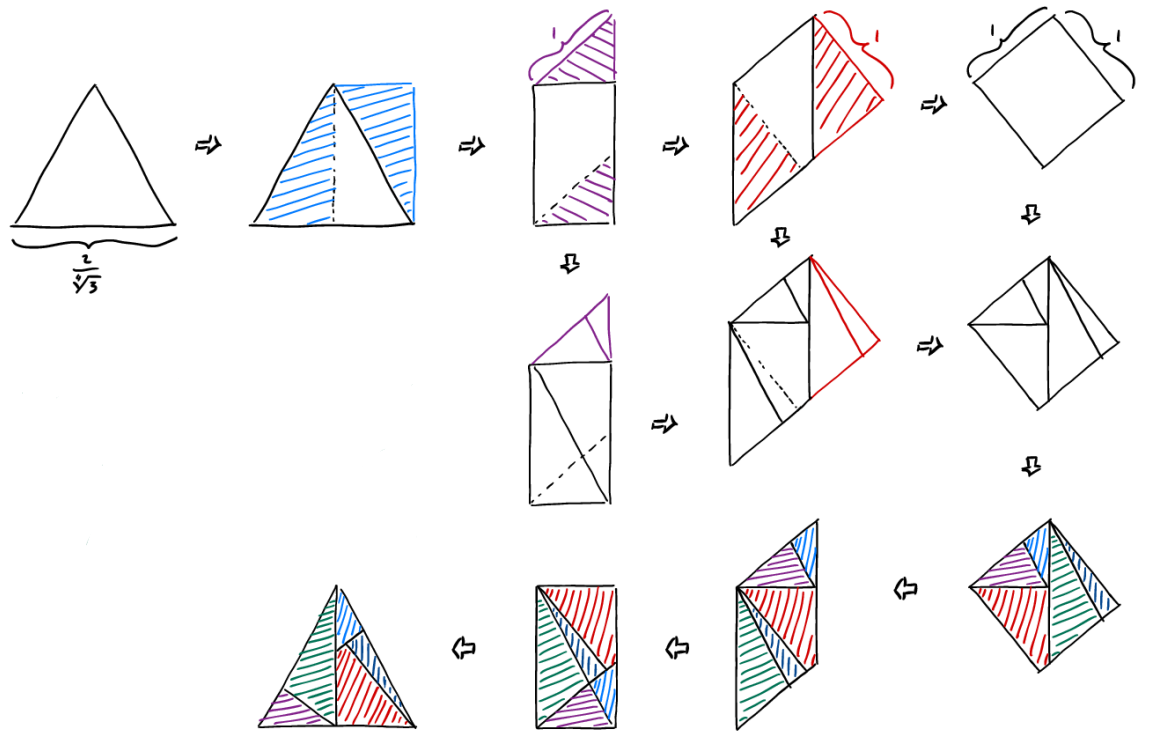
\includegraphics[width = 10cm]{immagini/Dehn_1.png}
\end{figure}

\textcolor{MidnightBlue}{Per passare da un poligono ad un quadrato equivalente [= con la stessa area], è sufficiente spezzarlo in triangoli, poi trasformare i triangoli in rettangoli, poi, passando per un parallelogramma, si trasforma un rettangolo in un altro con uno dei due lati arbitrario.
Infine, portando tutti i rettangoli ad avere un lato uguale, unendoli, e trasformando il nuovo rettangolo in un quadrato, di nuovo col trucco del parallelogramma, si ottiene appunto il quadrato desiderato.}

\begin{note}[L'area secondo Euclide]
	Curiosamente, \href{https://en.wikipedia.org/wiki/Euclid}{\textcolor{purple}{Euclide}} non definisce l'area, ma, dal momento che ci ragiona aggiungendo e togliendo pezzi congruenti, possiamo adattare, a posteriori, una definizione basata sull'equiscomponibilità alla matematica classica.
	Ancora più curiosamente, i ragionamenti di Euclide richiedono in realtà di definire $\text{Area}(A) = \text{Area}(B)$ se e solo se esistono due poligoni $C$ e $D$, rispettivamente non sovrapposti ad $A$ e $B$, equiscomponibili fra loro, tali che $A \cup C$ e $B \cup D$
	sono equiscomponibili. Per dedurre, che, in realtà, due poligoni con la stessa area sono equiscomponibili serve \href{https://en.wikipedia.org/wiki/Archimedean_property}{\textcolor{purple}{l'assioma di Archimede}} che Euclide non aveva. La sistemazione formale di questi concetti è dovuta 
	a \href{https://en.wikipedia.org/wiki/David_Hilbert}{\textcolor{purple}{Hilbert}}, e al XIX secolo.
\end{note}

Ebbene, tutti questi anacronismi solo per dire che \textcolor{purple}{in tre dimensioni questa definizione (per il volume in questo caso) non funziona}, ovvero non è detto che due poliedri con lo stesso volume si possano scomporre in parti congruenti (e quindi non possiamo ottenere l'uno dall'altro come nel caso bidimensionale).

\begin{theorem}[\href{https://en.wikipedia.org/wiki/Max_Dehn}{\textcolor{purple}{Dehn}}]
	Un cubo ed un tetraedro regolare, sia pure aventi il medesimo volume, non si possono scomporre in un numero finito di poliedri congruenti (cioè non sono equiscomponibili).\footnote{Questa proposizione
	e annessa dimostrazione sono un caso particolare della soluzione generale di Dehn al \href{https://en.wikipedia.org/wiki/Hilbert\%27s_third_problem}{\textcolor{purple}{terzo problema di Hilbert}}.}
\end{theorem}

\hspace{-0.43cm}\emph{Dimostrazione.} Supponiamo di avere una funzione $f : \RR \to \RR$ additiva tale che $f(x) = 0$ se e solo se $x$ è un multiplo razionale di $\pi$ - $x = k\pi$ con $k \in \QQ$.\\
	Definiamo il \vocab{valore} di un poliedro come la somma dei valori dei suoi spigoli, definiti, a loro volta, dicendo che il valore di uno spigolo di lunghezza $\ell$ che formi un angolo diedro di ampiezza $\alpha$ e $\ell \cdot f(\alpha)$.\\
	\begin{wrapfigure}[13]{r}{0.2\textwidth}
		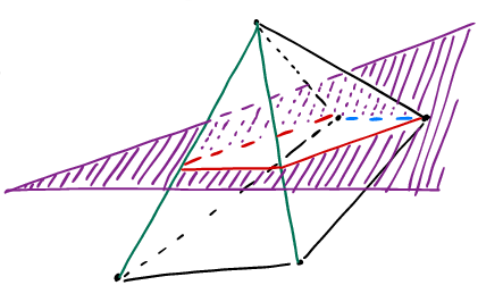
\includegraphics[width=0.17\textwidth]{immagini/cubo_tetraedro.png}
		\hspace{-0.2cm} 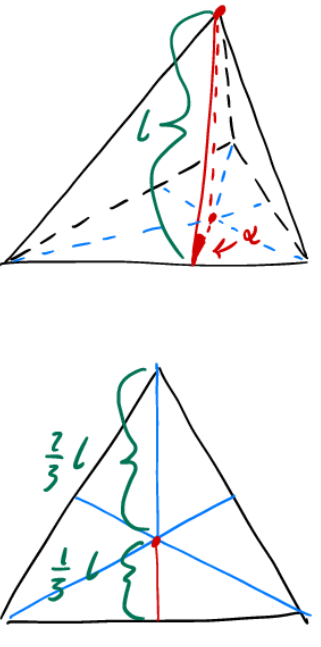
\includegraphics[width=0.13\textwidth]{immagini/angolo_diedro.png}
	\end{wrapfigure}
	Quando tagliamo un poliedro $A$ con un piano, ottenendo così due nuovi poliedri $B$ e $C$, la somma dei valori di $B$ e $C$ equivale al valore di $A$. Infatti, il taglio dà luogo ad alcuni spigoli nuovi, in \textcolor{red}{rosso}, ma la somma dei due angoli 
	diedri, poniamo $\alpha_1$ e $\alpha_2$, che insistono su uno qualunque di essi è $\pi$ e quindi vale che $\ell \cdot f(\alpha_1) + \ell \cdot f(\alpha_2) = \ell \cdot f(\alpha_1 + \alpha_2) = \ell \cdot f(\pi) \overset{\text{def. di $f$}}{=} 0$.\\
	Può dividere spigoli vecchi, in \textcolor{LimeGreen}{verde}, in due,
	poniamo di lunghezza $\ell_1$ e $\ell_2$, senza alterare l'angolo diedro, per cui $(\ell_1 + \ell_2) \cdot f(\alpha) = \ell_1 \cdot f(\alpha) + \ell_2 \cdot f(\alpha)$. Infine, in \textcolor{cyan}{azzurro}, può spezzare l'angolo diedro lasciando inalterata la lunghezza, e si conclude similmente.\\
	Abbiamo concluso quindi che il \vocab{valore} è invariante per equiscomposizioni, pertanto \textcolor{purple}{due figure equiscomponibili devono avere necessariamente lo stesso valore}, non ci resta che costruire $f$. Fissiamo una base $B$ di $\RR$ come spazio vettoriale su $\QQ$ tale che $\pi \in B$
	- ossia estendendo l'insieme linearmente indipendente $\{\pi\}$ (che è una applicazione diretta della proposizione dimostrata in precedenza).
	Definiamo:
	\[ f(\pi q_0 + b_1 q_1 + \ldots + b_n q_n) = b_1 q_1 + \ldots + b_nq_n
		\]
	per ogni $q_0,\ldots,q_n \in \QQ$ e $b_1,\ldots,b_n \in B \setminus \{\pi\}$ \textcolor{MidnightBlue}{- $f$ è quindi la proiezione su un completamento del sottospazio $\pi \QQ$ -}. L'additività di $f$ è conseguenza immediata della $\QQ$-linearità.
	Inoltre, per definizione, $f(x) = 0$ se e solo se $x = \pi q_0$, con $q_0 \in \QQ$.\\
	Ora è chiaro che il valore di un cubo è nullo, perché tutti i diedri hanno ampiezza $\frac{\pi}{2}$, quindi i valori dei singoli spigoli sono tutti nulli e così la loro somma (che per definizione è appunto il valore del cubo).\\
	Vediamo ora che il valore di un tetraedro regolare non è mai nullo - anche se il tetraedro avesse lo stesso volume del cubo -, in tal modo, per quanto detto sul valore, cubo e tetraedro non sono equiscomponibili.\\
	Si vede che gli angoli diedri del tetraedro valgono $\alpha = \arccos\frac 13$, quindi basta dire che questo $\alpha$ non è multiplo razionale di $\pi$, in tal modo il valore de tetraedro sarà non nullo. In altri termini,
	vogliamo verificare che, $n\alpha$, per $n \in \omega$, non è un multiplo intero di $\pi$.\\
	Questo fatto si può esprimere, altresì, dicendo che $z^n \not\in \RR$, dove $z = \cos \alpha + i \sin \alpha \in \CC$ - $z^n = \cos(n\alpha) + i \sin(n\alpha)$, dunque se $n\alpha$ fosse multiplo di $\pi$ si avrebbe $\Im(z^n) = 0 \implies z^n \in \RR$.
	Ora, avendo $\alpha = \arccos \frac 13$, $z = \frac{1}{3}(1 + 2i \sqrt 2)$, e, si vede immediatamente per induzione, che
	$(1 + 2i\sqrt 2)^n = x_n + y_n i \sqrt 2$ per qualche $x_n,y_n \in \ZZ$ (ci basta controllare che $y_n \ne 0$ per ogni $n$). Inoltre, sempre per induzione, riducendo $x_n$ e $y_n$ modulo 3, otteniamo che:
	\begin{itemize}
		\item per $n$ dispari $x_n \equiv 1 \pmod 3$ e $y_n \equiv 2 \pmod 3$.
		\item per $n$ pari e diverso da 0 invece $x_n \equiv 2 \pmod 3$ e $y_n \equiv 1 \pmod 3$.
	\end{itemize}
	In nessun caso, in particolare, si ottiene che $y_n \equiv 0 \pmod 3$, quindi non potrà essere mai che $y_n = 0$, pertanto $z^n$ non sarà mai reale e quindi $n\alpha$ mai multiplo razionale di $\pi$. \hfill $\square$
\newpage
\subsection{Insieme di Vitali}

Vediamo ora un'altra applicazione che da luogo ad un risultato negativo: il \vocab{controesempio di Vitali}.

\begin{definition}[Misura $\sigma$-additiva]
	Una \vocab{misura $\sigma$-additiva} su $\ps(\RR)$ è una funzione $\mu : \ps(\RR) \rightarrow \RR_{\geq 0}\cup\{+\infty\}$, tale che $\mu(\emptyset) = 0$ e, se $\{A_i\}_{i \in \omega}$ è 
	una successione di elementi \textcolor{red}{disgiunti} di $\ps(\RR)$ allora:
	\[ \mu\left(\bigcup_{i \in\omega} A_i\right) = \sum_{i = 0}^{+\infty} \mu(A_i)
		\]
\end{definition}

\begin{definition}[Misura invariante per traslazioni]
	Una misura $\mu$ si dice \vocab{invariante per traslazioni} se $\forall x \in \RR$ e $A \in \ps(\RR)$:
	\[ \mu(A) = \mu(\{y \in \RR | \underbrace{y - x \in A}_{\Mydef A + x}\})
		\]
	cioè la misura di un sottoinsieme di $\RR$ è invariante se lo trasliamo.
\end{definition}

\begin{remark}[Monotonia di una misura]
	Si osserva che se $A \subseteq B \subseteq \RR$, allora $\mu(A) \leq \mu(B)$.
\end{remark}

\begin{proof}
	Si vede che $\mu(B) = \mu(A \sqcup (B \setminus A)) \overset{\text{additività}}{=} \mu(A) + \mu(B \setminus A) \geq \mu(A)$.
\end{proof}

\begin{exercise}
	Esibisci una misura $\sigma$-additiva ed invariante per traslazioni su $\ps(\RR)$.
\end{exercise}

\begin{soln}
	La \href{https://en.wikipedia.org/wiki/Lebesgue_measure}{\textcolor{purple}{misura di Lebesgue}} è una misura $\sigma$-additiva ed invariante per traslazioni su $\ps(\RR)$.
\end{soln}

\begin{proposition}[Controesempio di Vitali]
	Non esiste una misura $\sigma$-additiva e invariante per traslazioni, $\mu : \ps(\RR) \to \RR_{\geq 0} \cup \{+\infty\}$, tale che $\mu([0,1[) = 1$.
\end{proposition}

\begin{proof}
	Supponiamo, per assurdo, che esista una tale misura $\mu$. Cerchiamo degli insiemi disgiunti $A_i \subseteq [0,1[$ con $i \in \omega$ tali che per ogni $i,j \in \omega$ $\mu(A_i) = \mu(A_j)$ e 
	$[0,1[\, = \bigcup_{i \in \omega} A_i$ - stiamo quindi cercando di partizionare $[0,1[$ con un numero numerabile di insiemi disgiunti e aventi tutti la stessa misura -. Se riusciamo scrivere una tale partizione otteniamo appunto un assurdo, infatti:
	\begin{itemize}
		\item se $\mu(A_i) = \mu(A_j) = 0$ per ogni $i,j \in \omega$, allora $\mu([0,1[) = \sum_{i \in \omega} \mu(A_i) = \sum_{i \in \omega}0 = 0 \ne 1 \; \textcolor{red}{\lightning}$.
		\item se $\mu(A_i) = \mu(A_j) = k > 0$ per ogni $i,j \in \omega$, allora $\mu([0,1[) = \sum_{i \in \omega} \mu(A_i) = \sum_{i \in \omega}k = k\cdot \sum_{i \in \omega} 1 = +\infty \ne 1 \; \textcolor{red}{\lightning}$.
	\end{itemize}
	Fissiamo $i \mapsto q_i$ un'enumerazione di $\QQ$, e fissiamo \textcolor{purple}{$B$ base di $\RR$} come $\QQ$-spazio vettoriale. Possiamo assumere WLOG che $b_0 = 1 \in B$, infatti, se così non fosse,
	ci basta prendere $b_0 \in B$ e moltiplicare tutti gli elementi di $B$ per $\frac{1}{b_0}$. Definiamo:
	\[ R_i := \{x \in \RR | x = \textcolor{MidnightBlue}{r_0} \cdot \textcolor{purple}{1} + \textcolor{LimeGreen}{q_i} \cdot \textcolor{purple}{b_1} + \textcolor{MidnightBlue}{r_2} \cdot \textcolor{purple}{b_2} + \ldots + \textcolor{MidnightBlue}{r_n} \cdot \textcolor{purple}{b_n},\;\text{con \textcolor{MidnightBlue}{$r_0,r_2,\ldots,r_n \in \QQ$}}\}
		\]
	cioè l'insieme dei reali che scritti in base $B$ hanno come coefficiente di $b_1$ l'$i$-esimo razionale. Definiamo inoltre $A_i := R_i \cap [0,1[$.
	Siccome la successione $(q_i)_{i \in \omega}$ enumera i razionali, l'unione degli $R_i$, al variare di $i \in \omega$, ci dà proprio - tutte le possibili scritture in base $B$ al variare dei coefficienti razionali - $\bigcup_{i \in \omega}R_i = \RR$,
	inoltre gli $R_i$ sono disgiunti per l'unicità della scrittura in base. Abbiamo quindi che la famiglia $\{R_i\}_{i \in \omega}$ è una partizione di $\RR$, e di conseguenza $\{A_i\}_{i \in \omega}$ è una partizione di $[0,1[$.\\
	Dimostriamo infine che $\mu(A_i) = \mu(A_j)$ per ogni $i,j \in \omega$. Siano $\delta :=(q_j - q_i)b_1$ e $k:=\lceil \delta \rceil$. Consideriamo l'insieme $A_i + \delta$, osserviamo in primis che si ha:
	\begin{align*}
		x \in R_i &\iff x \in \Span(B \setminus\{b_1\}) + q_ib_1 \\
				  &\iff x + \delta \in \Span(B \setminus\{b_1\}) + q_jb_1 &&\textcolor{MidnightBlue}{(q_jb_1 = \delta + q_ib_1)} \\
				  &\iff x + \delta \in R_j
	\end{align*}
	per cui possiamo scrivere $A_i+\delta$ come:
	\begin{align*}
		A_i + \delta &= (R_i + \delta) \cap [\delta,\delta + 1[ \\
					 &= R_j \cap [\delta,\delta + 1[ &&\textcolor{MidnightBlue}{(R_i + \delta = R_j)}\\
					 &= \underbrace{R_j \cap [\delta,k[}_{=: X_1} \cup \underbrace{R_j \cap [k,\delta + 1[}_{=: X_2}
	\end{align*}
	e naturalmente $X_1$ ed $X_2$ sono disgiunti. Similmente per $n \in \omega$:
	\begin{align*}
		x \in R_j &\iff x \in \Span(B \setminus\{b_1,1\}) + \QQ + q_jb_1 \\
				  &\iff x + n \in \Span(B \setminus\{b_1,1\}) + \QQ + q_jb_1 &&\textcolor{MidnightBlue}{(\QQ + n = \QQ)} \\
				  &\iff x + n \in R_j
	\end{align*}
	(in altre parole stiamo semplicemente assorbendo il termine in $\QQ$ nel coefficiente di $b_0 = 1$ nella scrittura in base). Possiamo quindi definire:
	\begin{align*}
		&Y_1 := X_1 - k + 1 = R_j \cap [\delta - k + 1, 1[ \\
		&Y_2 := X_2 - k = R_j \cap [0,\delta - k + 1[
	\end{align*}
	dove abbiamo usato che $R_j = R_j - k + 1$ e $R_j = R_j - k$ per l'osservazione vista prima.
	Di conseguenza $Y_1 \cap Y_2 \subseteq [\delta - k + 1, 1[ \, \cap \,[0,\delta - k + 1[ = \emptyset$ e $Y_1 \cup Y_2 = R_j \cap ([\delta - k + 1, 1[ \, \cup [0,\delta - k + 1[) = R_j \cap [0,1[ = A_j$.
	Mettendo tutto assieme segue quindi:
	\[ \mu(A_j) = \mu(Y_1) + \mu(Y_2) \overset{\text{invar. per trasl.}}{=} \mu(X_1) + \mu(X_2) = \mu(A_i + \delta) \overset{\text{invar. per trasl.}}{=} \mu(A_i)
		\]
\end{proof}

\begin{exercise}[Dimostrazione alternativa]
	Una maniera alternativa di dimostrare la proposizione precedente è come segue:
	\begin{itemize}
		\item considerare la relazione di equivalenza su $[0,1[$ data da $x \sim y \overset{\text{def}}{\iff} x - y \in \QQ$.
		\item fissare un $V \subseteq [0,1[$ che contiene un solo per ogni classe di equivalenza \textcolor{MidnightBlue}{- si usa AC}.
		\item dimostrare che $[0,1[ \subseteq S \Mydef \bigcup_{r \in \QQ \cap ]-1,1[} V + r \subseteq [-1,2[$, per cui $1 \leq \mu(S) \leq 3$.
		\item osservare tuttavia che se $\mu(V) = 0$ allora $\mu(S) = 0$ e se $\mu(V) > 0$ allora $\mu(S) = +\infty$.\footnote{Per la soluzione si veda \href{https://it.wikipedia.org/wiki/Insieme_di_Vitali}{\textcolor{purple}{qui}}.}
	\end{itemize}
\end{exercise}


\subsection{\texorpdfstring{\;Il teorema di Cantor-Bendixson}{Il teorema di Cantor-Bendixson}}
Il teorema di Cantor-Bendixson, che permette di dimostrare l'\vocab{ipotesi del continuo} limitatamente ai sottoinsiemi chiusi di $\RR$, non è tecnicamente, un'applicazione di AC.
Tuttavia è un esempio di come le tecniche insiemistiche - segnatamente la ricorsione transfinita - hanno conseguenze in matematica.\\
Come abbiamo osservato all'inizio del corso, quello di indagare la struttura dei sottoinsiemi chiusi di $\RR$ è stato, forse, uno dei problemi che hanno motivato lo sviluppo della teoria di Cantor. In 
questa sezione ne vedremo, in qualche misura la soluzione.

\paragraph*{Promemoria}\mbox{}\\
Se $S \subseteq \RR$ diciamo che $x \in \RR$ è un \vocab{punto di accumulazione} di $S$, se $x \in \ol{(S \setminus \{x\})}$ \textcolor{MidnightBlue}{- ossia (è nella chiusura di $S\setminus\{x\}$) se esiste una successione $(x_i)_{i \in \omega}$ di 
punti di $S \setminus \{x\}$ tale che $\lim_{i \to +\infty} x_i = x$}. Diciamo che $S \subseteq \RR$ è \vocab{perfetto} se $S$ coincide con l'insieme dei suoi punti di accumulazione ($\mathcal{D}(S)$, il \vocab{derivato} di $S$).

\begin{example}[Gli intervalli chiusi sono insiemi perfetti]
	Un intervallo chiuso $[a,b]$ è un esempio di insieme perfetto.
\end{example}

\begin{exercise}
	Esibire un insieme perfetto non vuoto avente \vocab{parte interna} - ossia $\{x \in S | \; \exists \varepsilon > 0 \; ]x -\varepsilon,x+\varepsilon[ \subseteq S\} = \mathring{S}$ - vuota.
\end{exercise}

\begin{soln}
	L'insieme di Cantor rispetta le proprietà richieste, infatti il suo complementare è unione di segmenti aperti, quindi è un aperto e dunque l'insieme di Cantor è un sottoinsieme chiuso dell'intervallo $[0,1]$.
	Inoltre in un qualsiasi intorno di un punto dell'insieme di Cantor ci sono sia punti dell'insieme sia punti del suo complementare, la prima cosa ci dice che tutti i punti sono aderenti, dunque è perfetto, la seconda ci dice che non ha punti interni,
	dunque ha parte interna vuota.
\end{soln}

\begin{proposition}[Sottoinsiemi perfetti di $\lbrack0,1\rbrack$]
	Se $S \subseteq [0,1]$ è perfetto, allora $|S| = 2^{\aleph_0}$
\end{proposition}

Per dimostrare questa proposizione, è comoda l'osservazione seguente.

\begin{remark}[Ogni perfetto di $\lbrack0,1\rbrack$ contiene due perfetti disugiunti]
	Se $S \subseteq [0,1]$ è perfetto e non vuoto allora esistono $S_1$ e $S_2$ sottoinsiemi di $S$ perfetti, non vuoti e disgiunti.
\end{remark}

\begin{proof}
	Un singoletto non è perfetto, quindi un perfetto ha almeno due punti, $x_1,x_2 \in S$, e supponiamo WLOG $x_1 < x_2$. Ora si danno due casi:
	\begin{itemize}
		\item \underline{se $[x_1,x_2] \subseteq S$}: consideriamo $x_3,x_4$ tali che $x_1 < x_2 < x_3 < x_4$ e definiamo $S_1 = S \cap [0,x_3], S_2 = S \cap [x_4,1]$, questi ultimi sono naturalmente disgiunti, non vuoti, chiusi e senza punti isolati
		(se ce ne fosse uno esisterebbe un intorno che lo isola ovvero che non sta nell'intersezione, ed essendo uno dei due intersecandi un intervallo chiuso l'unica possibilità è che l'intorno che isola il punto 
		nell'intersezione non stia nell'intervallo ma stia solo in $S$, tuttavia in tal modo il punto sarebbe isolato in $S$ che è perfetto $\lightning$).
		\item \underline{se esiste $x_3 \in [x_1,x_2]\setminus S$}: definiamo $S_1 = S \cap [0,x_3]$ e $S_2 = S \,\cap\, [x_3,1]$ (in questo caso intersecando con i chiusi otteniamo ancora un chiuso ed $x_3$ comunque non ci sta dentro, per cui vale lo stesso ragionamento di sopra\footnote{Typo Mamino-}).
	\end{itemize}
\end{proof}

Veniamo ora alla dimostrazione della proposizione.

\begin{wrapfigure}[7]{r}{0.16\textwidth}
	\vspace*{-0.8cm}
	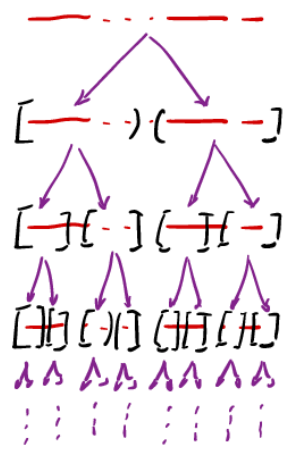
\includegraphics[width=0.15\textwidth]{immagini/perfetti di [0,1].png}
\end{wrapfigure}
\textcolor{MidnightBlue}{L'idea è quella di usare l'osservazione per dividere l'insieme $S$ in due, poi, ricorsivamente ciascuna delle due parti nuovamente in due, e coì via.
Si ottiene un albero binario di sottoinsiemi perfetti di $S$. Quest'albero ha ben $2^{\aleph_0}$ rami infiniti, uno per ogni successione di cifre binarie, e l'intersezione degli insiemi di ogni ramo 
è un'intersezione di compatti uno nell'altro, quindi non vuota. Per cui abbiamo una funzione iniettiva delle successione di cifre binarie a $S$.}

\begin{proof}
	Sia $P$ l'insieme dei sottoinsiemi perfetti di $[0,1]$. Fissiamo $f : P \to P \times P$ che manda $X \in P$ in una coppia $(X_1,X_2)$ con $X_1 \cup X_2 \subseteq X$ e $X_1 \cap X_2 = \emptyset$, e che è ben definita per l'osservazione precedente.\\
	Assegnamo ad ogni sequenza binaria finita, $\sigma : n \to \{0,1\}$, un sottoinsieme perfetto $S_\sigma$ di $S$, procedendo per ricorsione finita su $n$. A questo scopo, data $\sigma : n \to \{0,1\}$ 
	e $b \in \{0,1\}$ indichiamo con $\sigma \frown b$ la sequenza data da $\sigma \cup \{(n,b)\} : n+1 \to \{0,1\}$ - cioè la sequenza $\sigma$ allungata di un passaggio che fa $b$ -. Allora possiamo definire ricorsivamente:
	\[ S_0 = S \qquad S_{\sigma \frown b} = \begin{cases}
		X &\text{se $b = 0$} \\
		Y &\text{se $b = 1$}
	\end{cases}
	\qquad \text{dove $(X,Y) = f(S_\sigma)$}
		\]
	Data una stringa binaria infinita $\tau : \omega \to \{0,1\}$, definiamo infine l'intersezione di tutti i perfetti incontrati man mano che si scende nell'albero:
	\[ S_\tau = \bigcap_{\substack{\sigma = \tau_{|n} \\ n \in \omega}} S_\sigma
		\]
	Osserviamo che, per ogni successione $\tau$, $S_\tau \ne \emptyset$, infatti, per ogni $n \in \omega$, $S_{\tau_{|s(n)}} \subseteq S_{\tau_{|n}}$, poiché ad ogni passaggio aggiungiamo alla successione un perfetto contenuto nel precedente,
	quindi i compatti - siamo in $[0,1]$ quindi sono tutti limitati - non vuoti $S_{\tau_{|n}}$ costituiscono una successione decrescente, per cui - è un fatto topologico - la loro intersezione, che è $S_{\tau}$, è non vuota.\\
	Inoltre se $\tau \ne \rho$ allora $S_\tau \cap S_\rho = \emptyset$ - cioè stringe diverse corrispondono ad intersezioni diverse -, infatti, detto $n$ il minimo indice per cui
	$\tau_{|s(n)} \ne \rho_{|s(n)}$\footnote{Typo Mamino.} - senza perdita di generalità assumiamo $\tau_n = 0$ e $\rho_n = 1$ - abbiamo quindi $S_{\tau_{|s(n)}} = A$ e $S_{\rho_{|s(n)}} = B$ con $A \ne B$ e, per minimalità, $(A,B) = f(S_{\tau_{|n}}) = f(S_{\rho_{|n}})$,
	quindi, per la decrescenza, $S_\tau \subseteq A$ e $S_\rho \subseteq B$ sono disgiunti poiché $A \cap B = \emptyset$.\\
	In conclusione, per ogni $\tau \in 2^\omega$ possiamo scegliere un punto in $S_\tau$ e questa funzione è 
	iniettiva, quindi $2^{\aleph_0} \leq |S|$. D'altro canto $|S| \leq |\RR| = 2^{\aleph_0}$, quindi $|S| = 2^{\aleph_0}$.
\end{proof}

\begin{exercise}
	Dimostrare la proposizione con $\RR$ al posto di $[0,1]$.
\end{exercise}

\begin{exercise}
	In quali passaggi della dimostrazione precedente abbiamo fatto uso dell'assioma della scelta?
\end{exercise}

\begin{exercise}
	Dimostrare la proposizione senza fare uso di AC.
\end{exercise}

\begin{theorem}[Cantor-Bendixson]
	\label{Cantor_Bendixson}
	Sia $C \subseteq \RR$ chiuso. Allora $C = A \cup P$, con $|A| \leq \aleph_0$ e $P$ perfetto.
\end{theorem}

\textcolor{MidnightBlue}{Cioè ogni sottoinsieme chiuso di $\RR$ è unione di un perfetto e di una quantità al più numerabile di punti isolati.}

\begin{proof}
	Dato un sottoinsieme chiuso $C \subseteq \RR$ indichiamo con $X'$ l'insieme dei suoi punti di accumulazione:
	\[ X' = \{a \in \RR | \forall \varepsilon > 0 \; ]a - \varepsilon, a + \varepsilon[ \, \cap \, (X \setminus \{a\}) = \emptyset\}
		\]
	Chiaramente se $X$ è chiuso si ha proprio che i punti di accumulazione sono tutti meno quelli isolati:
	\[ X' = X \setminus \{\text{punti isolati di $X$}\}
		\]
	dove un punto $a \in X$ è isolato se $\exists \varepsilon > 0 \; ]a - \varepsilon, a + \varepsilon[ \, \cap \, X = \{a\}$. Ci servirà l'osservazione seguente: $a \in X$ è un punto isolato di $X$
	se e solo se esiste un intervallo $]s,t[$ aventi estremi razionali che isola $a \in X$, ossia:
	\[ \exists s,t \in \QQ \; s < t \;\land\; ]s,t[ \,\cap\, X  = \{a\}
		\]
	Definiamo ora una successione di sottoinsiemi chiusi a partire da $C$ per ricorsione transfinita come segue:
	\[ C_\alpha := \begin{cases}
		C_0 = C \\
		C_{\alpha + 1} = C_{\alpha}' \\
		C_{\lambda} = \bigcap_{\gamma < \lambda}C_\gamma
	\end{cases}
		\]
	cioè partiamo da $C$ e ad ogni passaggio prendiamo il suo derivato - i suoi punti di accumulazione -, al limite prendiamo semplicemente l'intersezione dei precedenti.
	Per vedere che tutti gli insiemi $C_\alpha$ sono chiusi basta osservare che il derivato di un chiuso è chiuso - di fatto stiamo soltanto togliendo punti isolati - e l'intersezione di chiusi è chiusa.
	Osserviamo inoltre che $\alpha \leq \beta \to C_\beta \subseteq C_\alpha$ - la successione è decrescente -. Definiamo quindi:
	\[ P := \bigcap_{\alpha \in \Ord} C_\alpha = \{a \in \RR | \forall \alpha \in \Ord \; a \in C_\alpha\}\footnote{Non è quindi una vera intersezione, ma un insieme definito per separazione.} \qquad A := C \setminus P
		\]
	Per verificare la tesi dobbiamo quindi dimostrare che $P$ è perfetto e $|A| \leq \aleph_0$.\\
	\textcolor{purple}{$P$ è perfetto}\\
	$P$ è chiuso poiché abbiamo osservato che i $C_\alpha$ sono chiusi e l'intersezione di chiusi è chiusa, occorre quindi dimostrare che $\forall a \in P$, $a$ è un punto di accumulazione per $P$.
	Procediamo per assurdo e consideriamo $a \in P$ isolato, sia $\varepsilon > 0$ tale che $P \,\cap\, ]a - \varepsilon, a + \varepsilon[ = \{a\}$. Per ogni $x \in ]a - \varepsilon, a + \varepsilon[ \setminus\{a\}$ siccome $x \not \in P$,
	esiste $\alpha$ tale che $x \not \in C_\alpha$ - cioè $x$ sta in un intervallo (bucato) che non sta in $P$, per cui non appartiene ad almeno un insieme dell'intersezione -, possiamo quindi prendere $\alpha_x$ minimo per cui $x \not \in C_{\alpha_x}$.
	Sia quindi:
	\[ \beta := \sup_{x \in ]a - \varepsilon, a + \varepsilon[ \setminus\{a\}} \alpha_x
		\]
	\textcolor{MidnightBlue}{cioè il più piccolo ordinale tale per cui $C_\beta$ non contiene alcun elemento di $x \in ]a - \varepsilon, a + \varepsilon[ \setminus\{a\}$}.
	In questo modo l'unico punto dell'intervallo che sta in $C_\beta$ è $a$ - perché per ipotesi sta in $P$, quindi in tutti i $C_\alpha$ -, cioè $C_\beta \,\cap\, ]a - \varepsilon, a + \varepsilon[ = \{a\}$, ma allora $a$ è un punto isolato per $C_\beta$ e quindi per definizione $a \not \in C_{s(\beta)}$, che implica $a \not \in P \;\textcolor{red}{\lightning}$.\\
	\textcolor{purple}{$A$ è al più numerabile}\\
	Per ogni $x \in A$ possiamo considerare $\alpha_x$, il minimo ordinale per cui $x \not \in C_{\alpha_x}$. Osserviamo che $\alpha_x$ deve essere successore,
	perché se fosse limite, avremmo $C_{\alpha_x} = \bigcap_{\gamma < \alpha_x} C_\gamma$, e, non stando nell'intersezione, esisterebbe $\gamma < \alpha_x$ per cui $x \not \in C_\gamma$ che è contro la minimalità di $\alpha_x$.
	Abbiamo quindi che $\alpha_x = s(\beta_x)$, per cui $C_{\beta_x}$ è l'ultimo elemento della successione che abbiamo costruito che contiene $x$.\\
	Siccome $x \in C_{\beta_x}$ e $x \not\in C_{s(\beta_x)} = C'_{\beta_x}$, ciò vuol dire che $x$ è un punto isolato per $C_{\beta_x}$. Per l'osservazione all'inizio possiamo quindi scegliere un intervallo a estremi razionali $]s_x,t_x[$ che isola $x$ in $C_{\beta_x}$.
	A questo punto ci basta definire la funzione:
	\[ A \to \QQ \times \QQ : x \mapsto (s_x,t_x)
		\]
	che è iniettiva. Infatti, siano $x,y \in A$ tali che $]s_x,t_x[ \,=\, ]s_y,t_y[$, supponiamo WLOG che $\beta_x \leq \beta_y$ - cioè $C_{\beta_x} \supseteq C_{\beta_y}$ -, allora:
	\[ y \in\, ]s_y,t_y[ \, \cap \, C_{\beta_y} \subseteq \, ]s_x,t_x[ \, \cap \, C_{\beta_x} = \{x\}
		\]
	dove il contenimento in mezzo vale perché stiamo supponendo gli intervalli uguali e prima abbiamo visto il contenimento dei $C_{\square}$, per cui $x = y$ e quindi abbiamo l'iniettività.
\end{proof}

\begin{corollary}[Vale l'ipotesi del continuo sui chiusi di $\RR$]
	Se $C \subseteq \RR$ è chiuso allora o $|C|=2^{\aleph_0}$ o $|C| \leq \aleph_0$.\footnote{Cioè tra $\aleph_0$ e $2^{\aleph_0}$ non c'è nulla per i chiusi di $\RR$.}
\end{corollary}

\begin{proof}
	Usando il teorema di Cantor-Bendixson scriviamo $C = A \cup P$. Se il perfetto è vuoto, $P = \emptyset$, allora $|C| = |A| \leq \aleph_0$.
	Altrimenti $2^{\aleph_0} = |P| \leq |C| \leq 2^{\aleph_0}$, dove la seconda disuguaglianza è perché $C \subseteq \RR$, mentre la prima uguaglianza 
	deriva dal fatto che abbiamo visto che i perfetti di $\RR$ hanno cardinalità $2^{\aleph_0}$.
\end{proof}

L'esempio seguente mostra come l'ipotesi che $C$ sia chiuso non possa essere omessa.

\begin{example}
	Esiste $S \subseteq \RR$ non numerabile che non contiene alcun insieme perfetto non vuoto.
\end{example}

\begin{proof}
	Sia $|\RR| = 2^{\aleph_0} = \aleph_\alpha$, e sia $f : \ps(\RR) \setminus\{\emptyset\} \to \RR$ una funzione di scelta per i sottoinsiemi di $\RR$. È evidente che:
	\[ 2^{\aleph_0} = |\{\text{intervalli chiusi}\}| \leq |\{\text{perfetti non vuoti}\}| \leq |\{\text{chiusi di $\RR$}\}| = 2^{\aleph_0}
		\]
	quindi esiste una funzione surgettiva - in realtà bigettiva - data da:
	\[ \omega_\alpha \twoheadrightarrow \{\text{perfetti non vuoti}\} : \beta \mapsto P_\beta
		\]
	Definiamo quindi:
	\[ g : \omega_\alpha \to \RR \times \RR : \beta \mapsto (g_1(\beta),g_2(\beta))
		\]
	dove $g_1$ e $g_2$ sono definite per ricorsione transfinita come segue:
	\begin{align*}
		&g_1(\beta) = f(P_\beta \setminus(g_1[\beta] \cup g_2[\beta])) \\
		&g_2(\beta) = f(\RR \setminus (g_1[\beta] \cup g_2[\beta] \cup \{g_1(\beta)\}))
	\end{align*}
	\textcolor{MidnightBlue}{Per cui $g_1$ prende un punto in $P_\beta$ che non sia già stato scelto in precedenza e $g_2$ prende un punto a caso tra quelli non scelti prima compreso $g_1(\beta)$.}\\
	La funzione $g$ è ben definita perché, per ogni $\beta < \omega_\alpha$, si ha $|\beta| < \aleph_\alpha$, quindi $|g_1[\beta]| \leq |\beta| < \aleph_\alpha$ e $|g_2[\beta]|\leq |\beta| < \aleph_\alpha$,
	d'altro canto - per quanto abbiamo visto in generale sui perfetti - $|P_\beta| = 2^{\aleph_0} = \aleph_\alpha$. Di conseguenza, per differenza di cardinalità, $f$ è sempre applicata ad insiemi non vuoti.\\
	Dimostriamo che $S := g_2[\omega_\alpha]$ soddisfa la tesi. In primis osserviamo che non è numerabile, infatti $g_2 : \omega_\alpha \to \RR$ è iniettiva perché, se WLOG $\gamma < \beta$, $g_2(\gamma) \in g_2[\beta]$ - ovvero il punto $g_2(\gamma)$ è nell'elenco di quelli già scelti quindi in $g_2[\beta]$ -
	e $g_2(\beta) = f(\RR \setminus (\ldots g_2[\beta] \ldots)) \ne g_2(\gamma)$ - cioè abbiamo scelto su un insieme dove non c'è $g_2(\gamma)$ -.
	Pertanto si ha $|g_2[\omega_\alpha]| = 2^{\aleph_0}$.\\
	Fissiamo ora un perfetto non vuoto $P_\beta$. Dobbiamo dimostrare che $P_\beta \not\subseteq g_2[\omega_\alpha]$. Ci basta dire che non c'è un suo punto, quindi ci basta mostrare che $g_1(\beta) \not \in g_2[\omega_\alpha]$.
	Supponiamo per assurdo $g_1(\beta) = g_2(\gamma)$ per qualche $\gamma \in \omega_\alpha$. Se $\gamma < \beta$ allora per le definizioni date:
	\[  g_1[\beta] \cup g_2[\beta] \not\ni g_1(\beta) = g_2(\gamma) \in g_1[\beta] \cup \,\textcolor{purple}{g_2[\beta]}\, \;\textcolor{red}{\lightning}
		\]
	Se $\beta \leq \gamma$:
	\[ g_1[\gamma] \cup g_2[\gamma] \cup \{g_1(\gamma)\} \not\ni g_2(\gamma) = g_1(\beta) \in \,\textcolor{purple}{g_1[\gamma]}\, \cup g_2[\gamma] \cup \{g_1(\gamma)\} \;\textcolor{red}{\lightning}
		\]
	quindi $g_1(\beta)$ non è immagine di qualche $\gamma \in \omega_\alpha$ per mezzo di $g_2$.
\end{proof}


\subsection{\texorpdfstring{\;Riepilogo forme equivalenti di AC}{Riepilogo forme equivalenti di AC}}
Abbiamo visto che diverse proposizioni sono equivalenti all'assioma della scelta. Per esempio, fissati gli altri assiomi, AC e 
l'affermazione che ogni insieme è bene ordinabile si implicano vicendevolmente. Elenchiamo le principali forme equivalenti dell'assioma della scelta.

\begin{proposition}[Forme equivalenti dell'assioma della scelta]
	Assumendo gli assiomi di: \hyperref[ax2]{estensionalità}, \hyperref[ax1]{insieme vuoto}, \hyperref[ax3]{separazione}, \hyperref[ax4]{paio}, \hyperref[ax5]{unione},
	\hyperref[ax6]{parti}, \hyperref[ax7]{infinito} e \hyperref[ax8]{rimpiazzamento} le seguenti proposizioni sono equivalenti:
	\begin{itemize}
		\item l'assioma della scelta
		\item ogni funzione surgettiva ha inversa destra
		\item il teorema del buon ordinamento
		\item il lemma di Zorn
		\item ogni cardinalità infinita è un aleph
		\item $\forall X,Y \; |X| \leq |Y| \lor |Y| \leq |X|$
		\item $\forall X \; |X| \leq |\aleph_0| \rightarrow |X \times X| = |X|$.
	\end{itemize}
\end{proposition}

\subsection{\texorpdfstring{\;$|X| = |X \times X| \rightarrow$ AC (Tarski)}{Teorema di Tarski sulla scelta}}
Della proposizione precedente ci rimane da dimostrare solo che per ogni insieme infinito $|X \times X| = |X|$ implica scelta.

\begin{theorem}[Teorema di Tarsk]
	Se per ogni $X$ infinito vale che $|X \times X| = |X|$, allora vale AC.
\end{theorem}

\begin{proof}
	Dato un $X$ infinito cerchiamo un buon ordinamento di $X$. È sufficiente costruire una funzione $g$ che immerge $X$ negli ordinali.\\
	Applicando l'ipotesi a $X \sqcup H(X)$ si ottiene:
	\[ |X \times H(X)| \leq |(X \sqcup H(X)) \times (X \sqcup H(X))| \overset{\text{Hp.}}{=} |X \sqcup H(X)|
		\]
	dove la prima disuguaglianza è una facile immersione\footnote{Ad esempio la mappa $(x,y) \mapsto ((x,0),(y,1))$ è iniettiva.}. Quindi esiste una funzione iniettiva $f : X \times H(X) \hookrightarrow X \sqcup H(X)$. Per ogni $a \in X$ consideriamo la funzione:
	\[ f_a : H(X) \rightarrow X \sqcup H(X) : b \mapsto f(a,b) \, \footnote{Moralmente $f_a = f(a,\cdot)$.}
		\]
	Se l'immagine $f_a[H(X)]$ di $f_a$ fosse contenuta in $X$ (cioè se gli elementi dell'immagine fossero tutte coppie con 0 alla seconda componente), allora avremmo una funzione iniettiva da $H(X)$ ad $X$, che è assurdo per la definizione di numero di Hartogs. Quindi accade necessariamente
	che $f_a[H(X)] \cap H(X) \ne \emptyset$. Definiamo:
	\[ g : X \rightarrow H(X) : a \mapsto \min(f_a[H(X)] \cap H(X))
		\]
	questa funzione è ben definita perché $f_a[H(X)] \cap H(X) \subseteq H(X)$, dunque è un insieme di ordinali, per il quale sappiamo esiste sempre il minimo. Inoltre $g$ è iniettiva perché, se $a \ne b$, allora $g(a) = f(a,\text{qualcosa})$ [per come è definita $f$], e per l'iniettività 
	di $f$, $f(a,\text{qualcosa}) \ne f(b,\text{qualcosa}) = g(b)$. Dunque $g$ è l'immersione cercata di $X$ negli ordinali, pertanto $X$ è bene ordinato, dunque segue il teorema del buon ordinamento e quindi l'assioma scelta.
\end{proof}
\section{Aritmetica cardinale}

\begin{definition}[Cardinali]
	Diciamo che $\kappa$ è un \vocab{cardinale} se $\kappa$ è un ordinale iniziale.
\end{definition}

\begin{notation}[Cardinali successori]
	Indichiamo con la notazione:
	\[ \kappa = \lambda^+ \Mydef \text{$\kappa$ è il minimo cardinale $>\lambda$}
		\]
	ad esempio, $\omega_\alpha^+ = \omega_{\alpha + 1}$, ovvero l'ordinale iniziale successivo [che quindi ha cardinalità strettamente più grande].
\end{notation}

Possiamo definire le operazioni di prodotto, somma e potenza cardinale (per il \hyperref[buon_ordinamento]{teorema del buon ordinamento} le operazioni sulle cardinalità e sugli ordinali iniziali corrispondono), per cui se $\kappa = \omega_\alpha$, $\lambda = \omega_\beta$ e $\mu = \omega_\gamma$ scriviamo:
\[ \kappa =  \lambda + \mu \qquad \kappa = \lambda \cdot \mu \qquad \kappa = \lambda^\mu
	\]
per rispettivamente:
\[ \aleph_\alpha = \aleph_\beta + \aleph_\gamma \qquad \aleph_\alpha = \aleph_\beta \cdot \aleph_\gamma \qquad \aleph_\alpha = \aleph_\beta^{\aleph_\gamma}
	\]
Occorre fare attenzione a non confondere le operazioni \textcolor{red}{cardinali} con quelle \textcolor{MidnightBlue}{ordinali}. In questa sezione ci occupiamo di operazioni \textcolor{red}{cardinali}.\\
Siccome ad ogni cardinalità corrisponde un unico ordinale iniziale [per \hyperref[ax9]{AC}], che abbia quella cardinalità, possiamo scrivere:
\[ \kappa = |X| \Mydef \text{$\kappa$ è un cardinale e $|\kappa| = |X|$}
	\]
Cioè stiamo commettendo un piccolo abuso di notazione (o di definizione) e dicendo che la definizione di cardinalità può essere in realtà quella dell'ordinale iniziale a lui associato, in realtà questa cosa non è sbagliata, nel senso che alla fine, tutte le cardinalità degli insiemi (per AC) sono ordinali iniziali, cioè vi è sempre una bigezione tra ordinale iniziale e insieme (se hanno la stessa cardinalità, ma la cardinalità, come detto in precedenza non è qualcosa di per sé, ma è una definizione che 
considera sempre due insiemi), quello che stiamo facendo con i cardinali non è altro che fissare una notazione per dei ``rappresentanti privilegiati'' delle cardinalità, che sono appunto gli ordinali iniziali.\\
Per questi ultimi valgono tutte le proprietà viste sulle cardinalità, che quindi ci danno le operazioni cardinali (che NON sono un'estensione di quelle ordinali, ma altre operazioni definite diversamente e soltanto tra ordinali iniziali, perché entrano in gioco le proprietà viste sulle cardinalità).\footnote{Osservare che nel caso degli ordinali [iniziali] finiti le operazioni ordinali coincidono con quelle cardinali ed entrambe coincidono con le operazioni definite per ricorsione numerabile su $\omega$, questo 
perché gli elementi di $\omega$ sono i loro stessi rappresentanti canonici di ordinali e sono tutti ordinali iniziali (per tutte le cardinalità finite).}
\subsection{Somme e prodotti infiniti}

\begin{definition}[Somme e prodotti infiniti]
	Sia $I$ un insieme e $\{\kappa_i\}_{i \in I}$ una famiglia di cardinali. Definiamo la \vocab{somma} e il \vocab{prodotto sulla famiglia} indicizzata da $I$ come:\footnote{La somma non è altro che una naturale estensione della somma tra cardinalità, per la somma di due cardinalità, in altre parole, stiamo rendendo disgiunti tutti gli insiemi e poi li stiamo unendo. Osservare anche che la definizione di prodotto data non usa AC.}
	 \begin{align*}
		\sum_{i \in I} \kappa_i &\Mydef\left\lvert \bigcup\{\kappa_i \times \{i\} | i \in I\}\right\rvert \\
		\prod_{i \in I} \kappa_i &\Mydef \left\lvert \left\{f : I \rightarrow \sup_{i \in I} \kappa_i \m  \forall i \in I \; f(i) \in \kappa_i\right\}\right\rvert 
	 \end{align*}
	(osservare che il sup di una famiglia di cardinali, essendo ordinali iniziali, è dato dall'unione di questi ultimi\footnote{Inoltre, notare anche come sapessimo già fare prodotti infiniti degli stessi insiemi, considerando le funzioni dall'uno all'altro, ma ciò valeva solo volendo fare un prodotto infinito di uno stesso insieme, per un numero di volte dato dall'insieme di arrivo
	(e.g. ${}^\omega A = \underbrace{A \times \ldots \times A}_{\text{$\omega$ volte}.}$).}).
\end{definition}

\textcolor{MidnightBlue}{Formalmente la famiglia $\{\kappa_i\}_{i \in I}$ è una funzione $f$ con $\Dom(f) = I$ e $\forall i \in I \; f(i)$ è un cardinale, $\kappa_i$ è un'abbreviazione per $f_i$.}

\begin{remark}[Prodotti cartesiani infiniti]
	La definizione sopra generalizza quella di prodotto cartesiano data, a prodotto cartesiano di una famiglia qualunque di insiemi qualunque. Nel caso finito c'è una bigezione tra le due definizioni, infatti, data una $f$ che va da $I$ all'unione $\bigcup \{X_i\}_{i \in I}$ [con $I$ finito] di una 
	famiglia di insiemi, tale $f$ per definizione fissa un elemento in ogni insieme, $f(i) \in X_i$, $\forall i \in I$, a questo punto, possiamo scrivere le immagini di $f(i)$ in una $|I|$-upla ordinata [secondo l'ordinamento su $I$], ed ottenere l'elemento del prodotto cartesiano finito voluto.\\
	Viceversa una $|I|$-upla definisce completamente una mappa da $I$ a $\bigcup\{X_i\}_{i \in I}$, infatti basta prendere come $f(i)$ l'$i$-esima componente della tupla, e tale componente sta in $X_i$, dunque si ottiene proprio una funzione che rispetta la proprietà richiesta.
\end{remark}

\begin{note}[Somma di cardinali disgiunti]
	Sia $\{X_i\}_{i \in I}$ una famiglia di insiemi a due a due \textbf{disgiunti}, e sia $\forall i \in I \; \kappa_i = |X_i|$\footnote{Se non sono già dati i cardinali c'è bisogno di AC.} allora:
	\[ \sum_{i \in I} \kappa_i = \left\lvert \bigcup\{X_i | i \in I\}\right\rvert 
		\]
	ovvero se gli insiemi a cui sono associati i cardinali sono disgiunti, la somma è semplicemente la cardinalità dell'unione senza bisogno di costruire l'unione disgiunta.\footnote{Questa proprietà così naturale nel caso finito, richiede AC per essere valida nel caso generale e dare una coerenza alle nostre definizioni, da qui l'importanza di assumere scelta per estendere le operazioni cardinali al caso infinito.}
\end{note}

\begin{proof}
	(Richiede \hyperref[ax9]{AC})\\
	Per ogni $i \in I$ scegliamo una bigezione $f_i : \kappa_i \times \{i\} \rightarrow X_i$, con $|\kappa_i \times \{i\}| = |\kappa_i| = |X_i|$\footnote{Per la precisione consideriamo $B = \{B_i\}_{i \in I}$, con $B_i = \{f_i : \kappa_i \times \{i\} \to X_i | \;\text{$f_i$ bigezione}$\},
	poiché per ogni $i \in I$ vale l'uguaglianza tra cardinalità scritta sopra, allora nessuno dei $B_i$ è vuoto, ovvero $\emptyset \not \in B$, dunque possiamo usare AC e ottenere una funzione $\phi : B \to \bigcup B : B_i \mapsto \phi(B_i) \in B_i$, che fissa per ogni insieme $B_i$ una sua bigezione.
	Osservare che usiamo AC per l'arbitrarietà di $|I|$, se fosse finito non avremmo bisogno di AC per fissare le bigezioni (per questo questa proprietà non ha bisogno di AC nel caso finito), ma nel caso infinito non possiamo fare altrimenti.}, allora si ha che:
	\[ f : \bigcup \{\kappa_i \times\{i\} | i \in I\} \rightarrow \bigcup \{X_i | i \in I\} : (a,i) \mapsto f_i(a,i)\,\footnote{Typo Mamino.}
		\]
	ossia $f = \bigcup\{f_i | i \in I\}$, ed è ben definita perché gli insiemi sono disgiunti inoltre è una bigezione perché unione di bigezioni definite su insiemi disgiunti in arrivo.
	Abbiamo quindi una bigezione tra l'insieme usato per la definizione di somma di cardinalità e l'unione degli insiemi corrispondenti a tali cardinalità, dunque la cardinalità dell'unione degli insiemi è proprio uguale alla somma delle cardinalità degli insiemi.
\end{proof}

\begin{note}[Disuguaglianza di inclusione-esclusione nel caso generale]
	Sia $\{X_i\}_{i \in I}$ una famiglia di insiemi non necessariamente a due a due disgiunti, e sia $\forall i \in I \; \kappa_i = |X_i|$\footnote{Come prima, se non sono già dati i cardinali c'è bisogno di AC.} allora in generale vale la disuguaglianza di inclusione-esclusione,
	ovvero la cardinalità dell'unione della famiglia è minore o uguale alla somma delle cardinalità degli elementi della famiglia:
	\[	\left\lvert\bigcup\{X_i | i \in I\} \right\rvert \leq \sum_{i \in I} \kappa_i
		\]
	Inoltre la definizione di prodotto data è ben posta indipendentemente dagli insiemi di cui si considera la cardinalità:
	\[ \prod_{i \in I} \kappa_i = \left\lvert\left\{f : I \to \bigcup_{i \in I} X_i \m \forall i \in I \; f(i) \in X_i\right\}\right\rvert 
		\]
\end{note}

\begin{proof}
	(Richiede \hyperref[ax9]{AC})\\
	Per la prima disuguaglianza si può fare come nel caso precedente, ovvero $\forall i \in I$ abbiamo $|\kappa_i \times \{i\}| = |X_i|$, per cui (usando AC nel caso generale) possiamo fissare una bigezione $f_i$, e considerare $f = \bigcup_{i \in I} f_i$, data da:
	\[ f : \bigcup\{\kappa_i \times \{i\} | i \in I\} \to \bigcup \{X_i | i \in I\} : (a,i) \mapsto f_i(a)
		\]
	in questo caso abbiamo che $f$ è unione di bigezioni, ma in arrivo gli insiemi non sono tutti necessariamente disgiunti, quindi ci può essere un elemento che ha più controimmagini, pertanto $f$ è soltanto surgettiva e tale surgettività ci dà:
	\[ \sum_{i \in I} \kappa_i = \left\lvert \bigcup\{\kappa_i \times \{i\} | i \in I\}\right\rvert \geq \left\lvert \bigcup \{X_i | i \in I\}\right\rvert 
		\]
	Per la seconda osservazione possiamo ancora una volta fissare per ogni $i \in I$ le bigezioni $g_i : \kappa_i \rightarrow X_i$ (con AC) e mandare ogni funzione del primo insieme in una funzione che valutata in ogni $i$ restituisce il valore di $f(i)$ trasportato in $X_i$ mediante la bigezione fissata per quell'$i$:
	\begin{align*}
		g : \left\{f : I \rightarrow \sup_{i \in I} \kappa_i \m \forall i \in I \; f(i) \in \kappa_i\right\} &\rightarrow \left\{f : I \rightarrow \bigcup \{X_i | i \in I\} \m \forall i \in I \; f(i) \in X_i\right\} \\
																								     f &\mapsto g(f)(i) = g_i(f(i))
	\end{align*}
	tale mappa è bigettiva, perché se due mappe in arrivo coincidono su tutti gli $i \in I$, essendo le $g_i$ bigezioni, si ha che le mappe in partenza sono uguali, inoltre presa una mappa $h$ nell'insieme in arrivo, si può ottenere la sua controimmagine costruendo una
	funzione fatta da $g_i^{-1}(h(i))$, per ogni $i \in I$.
\end{proof}

\begin{remark}[Prodotto infinito di potenze]
	Vale la proprietà del prodotto di potenze\footnote{$a^{n+m} = a^na^m$.} anche nel caso di prodotti arbitrari:
	\[ \kappa^{\sum_{i \in I}\lambda_i} = \prod_{i \in I} \kappa^{\lambda_i}
		\]
\end{remark}

\begin{proof}
	Un elemento dell'insieme al LHS è una funzione $f : \sum_{i \in I} \lambda_i = \bigcup\{\lambda_i \times \{i\} | i \in I\} \rightarrow \kappa$,
	tale funzione può essere identificata in una funzione:
	\[ \prod_{i \in I}\kappa^{\lambda_i}\ni\widetilde{f} : I \rightarrow \bigcup\{\kappa^{\lambda_i} | i \in I\} : i \mapsto \widetilde{f}_i \in \kappa^{\lambda_i}
		\]
	ovvero mandiamo $f$ in una funzione che associa ad ogni $i \in I$ la funzione $\widetilde{f}_i := f(\cdot,i) \in \kappa^{\lambda_i}$. È abbastanza immediato verificare che è iniettiva, infatti se due funzioni in arrivo coincidono praticamente le funzioni in partenza coincidono su tutte le coppie di elementi 
	in $\bigcup\{\lambda_i \times \{i\} | i \in I\}$, si verifica inoltre che è anche surgettiva.
\end{proof}

\begin{exercise}[Proprietà delle operazioni cardinali]
	Valgono le proprietà ragionevoli per le operazioni tra cardinali, ad esempio:
	\begin{itemize}
		\item se $\forall i \in I \; \kappa_i \leq \lambda_i$: \textcolor{orange}{(compatibilità con l'ordinamento - versione infinita)}
		\[ \sum_{i \in I} \kappa_i \leq \sum_{i \in I} \lambda_i \qquad \prod_{i \in I} \kappa_i \leq \prod_{i \in I} \lambda_i
			\]
		\item $\forall i \in I \; \kappa_i \leq \sum_{i \in I} \kappa_i$ \textcolor{orange}{(corollario di quella sopra)}
		\item Se $I = I_1 \sqcup I_2$: \textcolor{orange}{(associatività infinita)}
		\[ \sum_{i \in I} \kappa_i = \left(\sum_{i \in I_1} \kappa_i\right) + \left(\sum_{i \in I_2} \kappa_i\right) \qquad \prod_{i \in I}\kappa_i = \left(\prod_{i \in I_1} \kappa_i\right)\cdot\left(\prod_{i \in I_2} \kappa_i\right)
			\]
		\item \textcolor{orange}{(compatibilità tra le definizioni di operazioni cardinali)}:
		\[ \sum_{i \in \kappa} \lambda = \kappa \cdot \lambda \qquad \prod_{i \in \kappa} \lambda = \lambda^\kappa
			\]
		\item \textcolor{orange}{(prodotto di potenze)}:
		\[ \left(\prod_{i \in I}\kappa_i\right)^\lambda = \prod_{i \in I} \kappa_i^\lambda
			\]
	\end{itemize}
\end{exercise}


\pagebreak
\begin{proposition}[Somma infinita di cardinali]
	Supponiamo che $\{\kappa_i\}$, per $i \in I$ sia una famiglia di cardinali diversi da 0, allora:
	\[ \sum_{i \in I}\kappa_i = |I| \cdot \sup_{i \in I} \kappa_i = \max\left(|I|, \sup_{i \in I}\kappa_i\right)
		\]
\end{proposition}

\begin{proof}
	La seconda uguaglianza deriva dal fatto che le cardinalità sono tutte aleph, per cui vale la proprietà vista per il prodotto tra aleph. Per la prima dimostriamo le due disuguaglianze come segue [e concludiamo con Cantor-Bernstein].
	\begin{itemize}
		\item[$\boxed{\leq}$] Deriva facilmente dalle proprietà viste sopra:
		\[ \sum_{i \in I} \kappa_i \leq \sum_{i \in I} \sup_{i \in I}\kappa_i = |I| \cdot \sup_{i \in I} \kappa_i
			\]
		dove appunto, la prima disuguaglianza è esattamente la compatibilità della somma con l'ordinamento dei cardinali, mentre la seconda uguaglianza è la compatibilità tra le definizioni delle operazioni.
		\item[$\boxed{\geq}$] Siccome $|I| \cdot \sup_{i \in I} \kappa_i$ è il massimo fra $|I|$ e $\sup_{i \in I} \kappa_i$ [lo abbiamo già visto all'inizio], basta verificare che la somma al LHS è maggiore di entrambi separatamente.
		$\sum_{i \in I}\kappa_i \geq \sum_{i \in I} 1 = |I|$, dove la prima disuguaglianza è la compatibilità prodotto-ordinamento [applicata a cardinali $>0$ per ipotesi] e la seconda quella delle operazioni. L'altra disuguaglianza segue osservando che:
		\[ \forall j \in I \; \sum_{i \in I} \kappa_i \geq \kappa_j
			\]
		cioè tutta la famiglia è più piccola della somma, quindi deve esserlo anche il sup di tale famiglia.
	\end{itemize}
\end{proof}

\subsection{Teorema di König}

\begin{proposition}[Teorema di \href{https://en.wikipedia.org/wiki/Gyula_K\%C5\%91nig}{\textcolor{purple}{König}}]
	Se $\forall i \in I \; \kappa_i < \lambda_i$ allora:
	\[ \sum_{i \in I} \kappa_i < \prod_{i \in I} \lambda_i
		\]
\end{proposition}

\begin{proof}
	Dimostriamo che non può valere il $\geq$. Siano:
	\[ A := \bigcup\{\kappa_i \times \{i\} | i \in I\} \qquad B := \left\{f : I \rightarrow \sup_{i \in I} \lambda_i \m \forall i \in I \; f(i) \in \lambda_i\right\} 
		\]
	gli insiemi le cui cardinalità definiscono rispettivamente il prodotto della famiglia $\{\lambda_i\}_{i \in I}$ e la somma della famiglia $\{\kappa_i\}_{i \in I}$.
	Data una qualunque funzione $f : A \rightarrow B$\footnote{Typo di Mamino.} dobbiamo dimostrare che non può essere surgettiva (ovvero $\neg |B| \geq |A|$, cioè non è vero che la somma è maggiore o uguale al prodotto).
	Consideriamo la famiglia di funzioni tra i cardinali $\kappa_i$ e $\lambda_i$ definita via $f$ da:
	\[ f_i : \kappa_i \to \lambda_i : \alpha \mapsto (\underbrace{f(\alpha,i)}_{\in B})(i) \in \lambda_i
		\]
 	siccome per ipotesi $\kappa_i < \lambda_i$ le funzioni $f_i$ non possono essere surgettive per ogni $i \in I$, e ciò si traduce nel fatto che, per ogni $i \in I$, $\lambda_i \setminus\Imm(f_i) \ne \emptyset$.\\
	Per quanto detto $\emptyset \not \in \{\lambda_i \setminus\Imm(f_i)\}_{i \in I}$, dunque possiamo usare AC per fissare fissare un elemento in ciascun insieme $\lambda_i \setminus\Imm(f_i)$, in particolare possiamo
	scrivere una funzione che associa l'indice $i$ in $I$ al corrispettivo elemento fissato in $\lambda_i \setminus \Imm(f_i)$ come segue:
	\[ g : I \rightarrow \sup_{i \in I} \lambda_i : i \mapsto g(i) \in \lambda_i \setminus \Imm(f_i)
		\]
	osserviamo che $g \in B$ in quanto $g(i) \in \lambda_i$ per ogni $i \in I$, inoltre vale che che $g \not \in \Imm(f)$. Se, per assurdo, $g \in \Imm(f)$, allora [ricordando che $f$ è definita sulle coppie di $A$]
	abbiamo $g = f(\alpha,i)$, per qualche $(\alpha, i) \in A$, da cui [per estensionalità per funzioni]: 
	\[ g(i) = f(\alpha,i)(i) \overset{\text{def. $f_i$}}{=} f_i(\alpha) \in \Imm(f_i) \; \lightning
		\]
	che è assurdo in quanto $g(i) \in \lambda_i \setminus \Imm(f_i)$ per definizione. Abbiamo quindi verificato che c'è sempre un elemento di $B$, $g \not \in \Imm(f)$, che rende falsa la surgettività di una qualunque funzione.
	Poiché per AC le cardinalità sono totalmente ordinate, deve quindi valere necessariamente che all'inizio si ha $|A| < |B|$.
\end{proof}

\begin{example}[Disuguaglianza di Cantor]
	Osserviamo che applicando il teorema di König sui cardinali 1 e 2, sommati su una famiglia $\kappa$, si ottiene:
	\[ \kappa = \sum_{i \in \kappa} 1 \;\textcolor{red}{<}\; \prod_{i \in \kappa} 2 = 2^\kappa
		\]
	(dove le uguaglianze laterali sono la compatibilità delle definizioni delle operazioni), ovvero proprio il \hyperref[cantor]{teorema di Cantor} dimostrato in precedenza, che ora diventa un caso particolare del teorema di König.
\end{example}

\begin{example}[$2^{\aleph_0} \ne \aleph_\omega$]
	Osserviamo che vale:
	\[ \aleph_\omega = \max\left(\aleph_0, \sup_{i \in \omega} \aleph_i\right) = \sum_{i \in \omega} \aleph_i \;\textcolor{red}{<}\; \prod_{i \in \omega} \aleph_{i + 1} \leq \prod_{i \in \omega} \aleph_\omega = \aleph_\omega^{\aleph_0}
		\]
	dove abbiamo usato che $\aleph_i < \aleph_{i + 1}$ per la definizione ricorsiva della funzione degli aleph. Questa cosa ci permette di osservare che, se valesse $2^{\aleph_0} = \aleph_\omega$, allora:
	\[ 2^{\aleph_0} = \aleph_\omega < \aleph_\omega^{\aleph_0} = (2^{\aleph_0})^{\aleph_0} = 2^{\aleph_0} \; \lightning
		\]
\end{example}

\begin{exercise}[Facile]
	Se $2^{\aleph_0} = \aleph_{41}$, allora $\aleph_{41}^{\aleph_0} = \aleph_{41}$.
\end{exercise}

\begin{soln}
	Basta sfruttare che il prodotto di numerabili è numerabile, infatti:
	\[ \aleph_{41}^{\aleph_0} \overset{\text{Hp.}}{=} (2^{\aleph_0})^{\aleph_0} = 2^{\aleph_0} \overset{\text{Hp.}}{=} \aleph_{41}
		\]
\end{soln}

\begin{exercise}[Difficile]
	Se $2^{\aleph_0} = \aleph_{41}$, allora $\aleph_{42}^{\aleph_0} = \aleph_{42}$.
\end{exercise}

\begin{soln}
	La soluzione più breve usa la formula di Hausdorff, che vederemo alla fine del capitolo (sarebbe $(\kappa^+)^{\lambda} = \kappa^{\lambda} \cdot \kappa^+$), per la quale:
	\[ \aleph_{42}^{\aleph_0} \overset{\text{Hausdorff}}{=} \aleph_{41}^{\aleph_0} \cdot \aleph_{42} \overset{\text{Hp.}}{=} (2^{\aleph_0})^{\aleph_0} \cdot \aleph_{42} = 2^{\aleph_0} \cdot \aleph_{42} \overset{\text{Hp.}}{=} \aleph_{41} \cdot \aleph_{42} = \aleph_{42}
		\]
\end{soln}

\begin{exercise}[Pure peggio]
	Se $2^{\aleph_0} = \aleph_{1}$\footnote{Che è l'\vocab{ipotesi del continuo} (\vocab{CH}).}, allora $\aleph_{n+1}^{\aleph_0} = \aleph_{n+1}$, per $n \in \omega$.
\end{exercise}

\begin{soln}
	Si procede per induzione numerabile e usando la formula di Hausdorff.
	\begin{itemize}
		\item[$\boxed{\text{caso 0}}$] In questo caso $\aleph_1^{\aleph_0} = (2^{\aleph_0})^{\aleph_0} = 2^{\aleph_0} = \aleph_1$.
		\item[$\boxed{\text{caso successore}}$] Assumiamo $\aleph_{n+1}^{\aleph_0} = \aleph_{n+1}$ e dimostriamo che $\aleph_{n+2}^{\aleph_0} = \aleph_{n+2}$. Utilizzando la formula di Hausdorff:
		\[ \aleph_{n+2}^{\aleph_0} = \aleph_{n+1}^{\aleph_0} \cdot \aleph_{n+2} \overset{\text{Hp. indutt.}}{=} \aleph_{n+1} \cdot \aleph_{n+2} = \aleph_{n+2}
			\]
	\end{itemize}
\end{soln}

\pagebreak
\subsection{Cofinalità}

\begin{definition}[Cofinalità - v.1]
	Dato un cardinale infinito $\kappa$, la \vocab{cofinalità} di $\kappa$, $\cof(\kappa)$, è il minimo cardinale 
	$\mu$ per cui esiste una famiglia $\{\lambda_i\}_{i \in \mu}$ di cardinali tali che:
	\[ \forall i \in \mu \; \lambda_i < \kappa \qquad \text e \qquad \kappa = \sum_{i \in \mu} \lambda_i
		\]
\end{definition}

\textcolor{MidnightBlue}{In altri termini, $\cof(\kappa)$ è il \textcolor{red}{minimo numero di parti} $<\kappa$ [ovvero proprio $\mu$] in cui può essere diviso un insieme di cardinalità $\kappa$.}

\begin{example}[Cofinalità v.1 di alcuni cardinali noti]
	Vediamone alcuni esempi pratici di cofinalità v.1, tenendo conto che cerchiamo sempre il minimo numero di ``pezzi'' in cui dividere un cardinale, in modo tale che i ``pezzi'' abbiano cardinalità strettamente minore:
	\begin{itemize}
		\item $\cof(\aleph_0) = \aleph_0$, qualsiasi cosa più piccola sarebbe un cardinale finito, e dividere $\aleph_0$ in un numero finito di parti dà ancora parti di cardinalità $\aleph_0$, mentre usando $\aleph_0$ abbiamo tutti ``pezzettini'' finiti, la cui unione finita è finita, ma l'unione di $\aleph_0$ cardinali finiti dà proprio $\aleph_0$ per le proprietà viste:
		\[ \aleph_0 = \sum_{i < \aleph_0} 1 \leq \sum_{i < \aleph_0} n_i \leq \sum_{i < \aleph_0} \aleph_0 = \aleph_0 \cdot \aleph_0 = \aleph_0
			\]
		\item $\cof(\aleph_\omega) = \aleph_0$ in quanto:
		\[ \sum_{\alpha < \aleph_0} \aleph_\alpha = \aleph_\omega
			\]
		e se usassimo $|I|<\aleph_0$ (ovvero un cardinale finito), accadrebbe che:
		\[\sum_{\alpha \in I} \aleph_\alpha = \max\left(|I|,\sup_{\alpha \in I} \aleph_\alpha\right) = \aleph_{\max(I)} < \aleph_\omega
		\]
		\item $\cof(\aleph_{42}) = \aleph_{42}$ in quanto:
		\[ \aleph_{42} = \sum_{i \in I} \kappa_i \leq \sum_{i \in I} \aleph_{41} = \max\left(|I|,\aleph_{41}\right) \implies |I| = \aleph_{42}
			\]
		dove la prima uguaglianza è il fatto che stiamo supponendo di poter scrivere $\aleph_{42}$ come somma, la seconda disuguaglianza deriva dal fatto che stiamo supponendo (per avere la definizione di cofinalità v.1) che i cardinali che sommiamo siano strettamente più piccoli di $\aleph_{42}$, e, nel caso peggiore (perché gli $\aleph_{41}$ sono i pezzi di
		grandezza massima che possiamo prendere), troviamo calcolando la somma, che 
		l'unica possibilità è che $|I| = \aleph_{42}$.
	\end{itemize}
\end{example}

\begin{definition}[Cofinalità - v.2]
	Dato un insieme ordinato $(S,<)$\footnote{Questa definizione di cofinalità, al contrario della precedente è valida su qualsiasi insieme [parzialmente] ordinato, mentre la
	precedente solo per i cardinali.}, diciamo che $A\subseteq S$ è \vocab{cofinale} in $S$ se $\forall x \in S \; \exists y \in A \; x \leq y$ \textcolor{MidnightBlue}{- ossia $A$ non 
	ha maggioranti stretti in S}. La \vocab{cofinalità} di $(S,<)$ è la minima cardinalità di un sottoinsieme cofinale di $S$.
\end{definition}

\begin{example}[Cofinalità v.2 di alcuni cardinali noti]
	Vediamone alcune secondo questa nuova definizione:
	\begin{itemize}
		\item $\cof(\omega) = \aleph_0$, $\omega$ è banalmente cofinale in se stesso, inoltre, qualsiasi altro sottoinsieme è finito, dunque ha un maggiorante stretto in $\omega$, pertanto $\omega$ è un\footnote{Va bene qualsiasi altro sottoinsieme infinito di $\omega$, tanto sono tutti $\aleph_0$.} sottoinsieme
		cofinale di $\omega$, da cui considerando la cardinalità si ha $\aleph_0$.
		\item $\cof(\RR,<) = \aleph_0$, infatti $\omega$ è cofinale in $\RR$, basta prendere per ogni $x \in \RR$ la parte intera superiore, $x \leq \lceil x \rceil \in \omega$, inoltre, per quanto visto con AC $\aleph_0$ è la più
		piccola cardinalità infinita (stiamo escludendo con lo stesso ragionamento di sopra che vi siano insiemi cofinali finiti in $\RR$), quindi per la definizione v.2, la minima cardinalità cercata è proprio $\aleph_0$.
		\item $\cof(]0,1],<_{|\RR}) = 1$, perché $\{1\}$ è un sottoinsieme cofinale di $]0,1]$ (non ha maggioranti stretti nel nostro intervallo), e la cofinalità non può essere 0 perché nell'intervallo ha maggioranti stretti.
		\item $\cof(\omega+1) = 1$, infatti, il sottoinsieme $\{\omega\} \subset \omega + 1$ non ha maggioranti stretti, per cui è cofinale ed in particolare $|\{\omega\}| = 1$, dunque, non essendo il vuoto (o 0) cofinale in $\omega + 1$, segue necessariamente che $\{\omega\}$ è il più piccolo sottoinsieme cofinale.
		\item $\cof(\omega_\omega) = \aleph_0$ perché $\{\omega_0,\omega_1,\omega_2,\ldots\} = \{\omega_\alpha | \alpha < \omega\}$ è un insieme cofinale in $\omega_\omega = \sup_{i \in \omega} \omega_\alpha$ [banalmente perché abbiamo preso tutti gli $\omega_\alpha$ prima di $\omega_\omega$, quindi non ci può essere fuori qualcosa di strettamente più grande], inoltre, la cardinalità di questo insieme è ovviamente $\aleph_0$,
		ed è il più piccolo insieme cofinale, infatti, per qualsiasi sottoinsieme finito di $\omega_\omega$, è sufficiente prendere il successivo dell'$\omega_\alpha$ più grande.
		\item $\cof(\omega_{42}) = \aleph_{42}$ per la proposizione che segue.
	\end{itemize}
\end{example}

\begin{proposition}[Equivalenza delle definizioni di cofinalità]
	Dato $\kappa$ cardinale \textbf{infinito}\footnote{Nel caso $\kappa$ cardinale finito, non coincidono, ed anzi, la definizione v.1 dà sempre 2, mentre la v.2 dà sempre 1, perché ogni cardinale finito ha sempre un massimo.},
	allora vale che $\cof^{\text{(v.1)}}(\kappa) = \cof^{\text{(v.2)}}(\kappa)$.
\end{proposition}

\begin{proof}
	Siano $\lambda_1 := \cof^{\text{(v.1)}}(\kappa)$ e $\lambda_2 := \cof^{\text{(v.2)}}(\kappa)$, verifichiamo quindi le due disuguaglianze per avere la tesi.
	\begin{itemize}
		\item[$\boxed{\lambda_1 \leq \lambda_2}$] Sia $A$ un sottoinsieme cofinale in $\kappa$, mostriamo che $\lambda_1 \leq |A|$, cioè che $\lambda_1$ è più piccolo di tutte le cardinalità dei sottoinsiemi cofinali di $\kappa$ in questo modo sarà proprio minore o uguale del minimo, ovvero $\lambda_2$.\\
		Osserviamo che (questo vale per tutti gli ordinali limite), essendo $\kappa$ un ordinale iniziale, dunque limite, $\forall \alpha \in \kappa \; \exists \beta \in A \; s(\alpha) \leq \beta$ (per cofinalità di $A$) e quindi $\alpha < \alpha + 1 \leq \beta$, dove $\alpha + 1 \in \kappa$ perché limite. Dunque ogni elemento di $\kappa$
		appartiene a qualche elemento di $A$, per cui vale $\kappa = \bigcup A$\footnote{Per essere precisi questo è un solo contenimento, l'altro segue dal fatto che $A \subseteq \kappa$ e $\kappa$ è un insieme transitivo, quindi $\bigcup A \subseteq \kappa$.}. Da ciò segue che:
		\[ \kappa \leq \sum_{\beta \in A} |\beta| \leq \sum_{\beta \in A} \kappa = |A| \cdot \kappa = \kappa
			\]
		per cui il termine in mezzo è uguale a $\kappa$, ed essendo che $\forall \beta \in A \; \beta \in \kappa \to |\beta| < \kappa$ (poiché $\kappa$ iniziale), quella ottenuta sopra è proprio una scrittura di $\kappa$ come somma di termini strettamente più piccoli, per cui si ha $ \lambda_1 \leq |A|$.
		\item[$\boxed{\lambda_2 \leq \lambda_1}$] Se $\lambda_1 = \kappa$ non c'è niente da dimostrare, perché $\kappa$ stesso è cofinale in sé, e quindi il minimo nella definizione v.2 comprende già $\kappa$ per cui la disuguaglianza è automaticamente verifica. Assumiamo quindi che $\lambda_1 < \kappa$, ci basta trovare un insieme cofinale in $\kappa$ di cardinalità $\lambda_1$, in questo modo sta nel minimo dell'altra definizione e otteniamo la disuguaglianza voluta.
		Per ipotesi esiste $\{\kappa_i\}_{i \in I}$ con $|I| = \lambda_1$, tale che per la definizione di cofinalità v.1:
		\[ \kappa = \sum_{i \in I} \kappa_i = \max\left(|I|,\sup_{i \in I} \kappa_i\right) = \max\left(\lambda_1, \sup_{i \in I} \kappa_i\right) \overset{\lambda_1 < \kappa}{=}\, \footnote{Se il max fosse $\lambda_1$, avremmo $\kappa = \lambda_1$, che è contro il fatto supposto poco sopra, ovvero $\lambda_1 < \kappa$, pertanto il max deve essere necessariamente il sup.} \sup_{i \in I} \kappa_i
			\]
		Osserviamo ora che $A := \{\kappa_i | i \in I\}$ è cofinale in $\kappa$ e da questo segue la tesi in quanto $\lambda_2 \overset{\text{def. cof$^{\text{(v.2)}}$}}{\leq} |A| \overset{i \twoheadrightarrow \kappa_i}{\leq} |I| = \lambda_1$.
		Dato $x \in \kappa$, se $x$ non fosse maggiorato da qualche elemento di $A$, avremmo che $x$ è un maggiorante di $A$ stesso, per cui:
		\[ \sup_{i \in I}\kappa_i \leq x < \kappa \; \lightning
			\]
		dove l'assurdo deriva dal fatto che sopra avevamo ottenuto che $\kappa = \sup_{i \in I}\kappa_i$. Alternativamente si può anche osservare che $x \in \kappa = \sup_{i \in I}\kappa_i = \bigcup_{i \in I}\kappa_i \left(= \bigcup A\right)$, ovvero $x \in \kappa_i$, per qualche $i \in I$, per cui $x < \kappa_i$, e dunque $A$ è cofinale in $\kappa$.
	\end{itemize}
\end{proof}

\begin{proposition}[Transitività della cofinalità]
	Sia $(S,<_S)$ totalmente ordinato e $T \subseteq S$ cofinale in $S$, allora:
	\[ \cof(S,<_S) = \cof(T,<_T)
		\]
	con $<_T = <_S \cap (T \times T)$.
\end{proposition}

\begin{proof}
	Per dimostrare la proposizione dimostriamo due cose, in primis che se $A \subseteq T$ è cofinale in $T$, allora è cofinale anche in $S$, dunque i sottoinsiemi cofinali di $T$ sono contenuti in quelli di $S$, per cui, per definizione v.2, si ha $\cof(S,<_S) \leq \cof(T,<_T)$.
	\begin{itemize}
		\item Dato $A \subseteq T$ cofinale in $T$, verifichiamo che è cofinale anche in $S$. Sia $x \in S$, dobbiamo trovare un $y \in A$ tale che $x \leq y$. Siccome $T$ è cofinale in $S$ per ipotesi, esiste $t \in T$ tale per cui $x \leq t$, e, siccome 
		$A$ è cofinale in $T$, esiste $y \in A$ per il quale $t \leq y$, da cui $x \leq y$.
	\end{itemize}
	La seconda cosa che dimostriamo è che se $B \subseteq S$ è cofinale in $(S,<_S)$, allora esiste un sottoinsieme $B' \subseteq T$, con $|B'| \leq |B|$, cofinale in $T$, in tal modo per la definizione v.2, si ha $\cof(T,<_T) \leq \cof(S,<_S)$, e si conclude la tesi.
	\begin{itemize}
		\item Dato $B \subseteq S$ cofinale, siccome $T$ è cofinale in $S$, possiamo usare la cofinalità di quest'ultimo rispetto a $B$, e quindi per ogni $b \in B \subseteq S$ possiamo fissare (in generale con AC) un $y_b \in T$ con $b \leq y_b$. Sia $B' := \{y_b \in T : b \in B\} \subseteq T$.\\
		Naturalmente la mappa $b \mapsto y_b$ è una funzione surgettiva da $B$ a $B'$, per cui abbiamo $|B'| \leq |B|$. Infine, non ci resta che osservare che $B'$ è cofinale in $T$, preso dunque $x \in T$, poiché $B$ è cofinale in $S$ esiste $b \in B \; b \geq x$,
		possiamo quindi considerare l'$y_b \in B'$ associato e ottenere $y_b \geq b \geq x$, che ci garantisce la cofinalità.
	\end{itemize}
\end{proof}

\begin{proposition}[I cardinali infiniti sono sempre cofinali in se stessi]
	Sia $\kappa$ un cardinale infinito, allora vale che $\cof(\kappa) \leq \kappa$.\footnote{Usando la definizione v.2, questo fatto è vero per un qualsiasi ordinale parziale.}
\end{proposition}

\begin{proof}
	Infatti, $\kappa$ si può scrivere come:
	\[ \kappa = \sum_{i \in \kappa} 1
		\]
	che rispetta la definizione v.1 di cofinalità. Pertanto $\kappa$ è tra le cardinalità di cui si prende il minimo nella definizione, e, essendo un elemento
	del minimo segue anche che necessariamente il minimo sara più piccolo, da cui $\cof(\kappa) \leq \kappa$.\\
	Ragionamento analogo se si usa la definizione v.2 di cofinalità, infatti ogni insieme è cofinale in se stesso, per cui $\kappa$ è tra gli insiemi di cui si considera il minimo della cardinalità per avere la cofinalità secondo questa definizione.
\end{proof}

\begin{remark}[La cofinalità è sempre un cardinale regolare]
	Sia $(S,<)$ totalmente ordinato, allora:
	\[ \cof(\cof(S,<)) = \cof(S,<)
		\]
	in particolare, per ogni cardinale infinito $\kappa$, si ha $\cof(\cof(\kappa)) = \cof(\kappa)$.
\end{remark}

\begin{proof}
	Sia $\kappa = \cof(S,<)$ e $A \subseteq S$ cofinale, quindi $|A| = \kappa$, sappiamo che vale in generale $\cof(\kappa) \leq \kappa$. Supponiamo per assurdo che $\cof(\kappa) < \kappa$,
	per definizione di cofinalità esistono $\{\kappa_i\}_{i \in I}$, $\forall i \in I \; \kappa_i < \kappa$ e $\cof(\kappa) = |I| < \kappa$, tali che:
	\[ \kappa = \sum_{i \in I} \kappa_i = |I| \cdot \sup_{i \in I}\kappa_i = \sup_{i \in I}\kappa_i
		\]
	dunque che possiamo fissare una famiglia $\{A_i\}_{i \in I}$ di sottoinsiemi di $A$ disgiunti tali che $\forall i \in I \; |A_i| = \kappa_i$ e $\bigcup\{A_i | i \in I\} = A$ (è l'osservazione vista all'inizio per cui data una famiglia arbitraria di insiemi disgiunti, la cardinalità della loro unione è proprio la somma dei cardinali associati).\\
	Osserviamo ora che ogni $i \in I$, $A_i$ \textcolor{red}{non è cofinale in $S$} siccome $|A_i| = \kappa_i < \kappa = \cof(S,<)$, quindi possiamo scegliere per tutti gli $A_i$ un maggiorante stretto $y_i \in S$.
	Sia $B := \{y_i \in S | i \in I\} \subseteq A$\footnote{Typo di Mamino.}, vale che $|B| \overset{i \twoheadrightarrow y_i}{\leq} |I| \overset{\text{Hp. assurda}}{<} \kappa$.\\
	D'altro canto $B$ è cofinale \textcolor{red}{in $S$}, infatti, preso $x \in S$, per la cofinalità di $A$,
	$\exists a \in A$ tale che $x \leq a$, ora $a$ è necessariamente in uno degli $A_i$, quindi si ha $x \leq a \leq y_i \in B$.
	Ma allora $B$ è cofinale in $(S,<)$ e ciò è assurdo perché $\cof(S,<) = \kappa$ e vale la disuguaglianza scritta sopra.
\end{proof}

Vediamo ora alcune applicazioni della cofinalità.

\begin{corollary}[di König - o disuguaglianze di cofinalità]
	Per $\kappa$ cardinale infinito, e $\lambda$ cardinale $\geq 2$ vale:
	\[ \kappa < \kappa^{\cof(\kappa)} \qquad \kappa < \cof(\lambda^{\kappa})\,
		\]
\end{corollary}

\begin{proof}
	Cominciamo dalla prima disuguaglianza. Per definizione di $\cof(\kappa)$ esiste una famiglia $\{\kappa_i\}_{i \in \cof(\kappa)}$, con $\kappa_i < \kappa$ per ogni $i \in \cof(\kappa)$, dunque usando König si ha:
	\[ \kappa = \sum_{i \in \cof(\kappa)} \kappa_i \; \textcolor{red}{<} \; \prod_{i \in \cof(\kappa)} \kappa = \kappa^{\cof(\kappa)}
		\]
	Per la seconda disuguaglianza ragioniamo per assurdo e assumiamo che $\kappa \geq \cof(\lambda^\kappa)$. A questo punto possiamo applicare la disuguaglianza precedente a $\lambda^\kappa$ ed ottenere:
	\[ \lambda^\kappa \;\textcolor{red}{<}\; (\lambda^\kappa)^{\cof(\lambda^\kappa)} \overset{\text{Hp. assurda}}{\leq} (\lambda^{\kappa})^{\kappa} = \lambda^{\kappa \cdot \kappa} = \lambda^{\kappa} \;\lightning
		\]
\end{proof}

\begin{definition}[Funzione $\gimel$]
	La funzione $\gimel$\footnote{\;``Gimel'', pronunciata ``ghimel''.} è definita sui cardinali infiniti da:
	\[ \gimel(\kappa) = \kappa^{\cof(\kappa)}
		\]
\end{definition}

\begin{corollary}[Disuguaglianze di cofinalità via $\gimel$]
	Con la funzione $\gimel$, dato $\kappa$ cardinale infinito, abbiamo le disuguaglianze di cofinalità:
	\[ \kappa < \gimel(\kappa) \qquad \cof(\kappa) < \cof(\gimel(\kappa))
		\]
\end{corollary}

\begin{proof}
	La prima disuguaglianza è una riscrittura di quella sopra, infatti $\kappa < \kappa^{\cof(\kappa)} = \gimel(\kappa)$. La seconda disuguaglianza è un corollario della seconda disuguaglianza sopra che
	si ottiene prendendo $\lambda = \kappa$ ed usando $\cof(\kappa)$ al posto di $\kappa$.
\end{proof}

\begin{definition}[Proprietà dei cardinali]
	Dato un cardinale $\kappa$, diciamo che è:
	\begin{itemize}
		\item \vocab{regolare} se $\cof(\kappa) = \kappa$
		\item \vocab{singolare} se $\cof(\kappa) < \kappa$
		\item \vocab{successore} se $\kappa = \aleph_{\alpha + 1}$ per qualche $\alpha \in \Ord$
		\item \vocab{limite} se $\kappa = \aleph_{\lambda}$ per $\lambda$ ordinale limite
		\item \vocab{limite forte} se $\aleph_0 < \kappa$ e $\forall \alpha \in \Ord \; \aleph_\alpha < \kappa \rightarrow 2^{\aleph_\alpha} < \kappa$
		\item \vocab{debolmente inaccessibile} se è regolare e limite
		\item \vocab{(fortemente) inaccessibile} se è regolare e limite forte.
	\end{itemize}
\end{definition}

\begin{proposition}[Limite forte $\implies$ limite]
	Un cardinale limite forte è anche limite.
\end{proposition}

\begin{proof}
	Se per assurdo fosse successore, $\kappa = \aleph_{\alpha + 1}$, poiché $\aleph_\alpha < \aleph_{\alpha + 1}$ avremmo per ipotesi di limite forte che $2^{\aleph_\alpha} < \aleph_{\alpha + 1}$, ma questo è assurdo in quanto $\aleph_{\alpha + 1} \leq 2^{\aleph_\alpha}$ poiché è per definizione il più piccolo cardinale strettamente maggiore di $\aleph_{\alpha}$.
\end{proof}

\begin{proposition}[Successore $\implies$ regolare]
	I cardinali successori sono regolari.
\end{proposition}

\begin{proof}
	Sia $\kappa = \aleph_{\alpha + 1}$, da sopra sappiamo che vale sempre $\cof(\kappa) \leq \kappa$, supponiamo per assurdo che $\kappa$ non sia regolare, cioè $\cof(\kappa) < \kappa$. Usando la definizione di cofinalità si ottiene:
	\[ \aleph_{\alpha + 1} = \kappa = \sum_{i \in \cof(\kappa)} \kappa_i \leq \sum_{i \in \cof(\kappa)} \aleph_\alpha = \cof(\kappa) \cdot \aleph_\alpha \leq \aleph_\alpha \;\textcolor{red}{<}\; \aleph_{\alpha + 1} \; \lightning
		\]
	dove nella penultima disuguaglianza abbiamo usato che $\cof(\kappa) < \kappa = \aleph_{\alpha + 1} \implies \cof(\kappa) \leq \aleph_\alpha$, poiché $\aleph_\alpha$ è il più grande cardinale strettamente più piccolo di $\aleph_{\alpha + 1}$.
\end{proof}

\begin{corollary}[$\gimel$ di cardinali regolari]
	Se $\kappa$ è \textcolor{red}{successore}, allora $\gimel(\kappa) = 2^{\kappa}$.
\end{corollary}

\begin{proof}
	È ovvio che $\gimel(\kappa) = \kappa^{\cof(\kappa)} \overset{\text{$\kappa$ regolare}}{=} \kappa^\kappa = 2^{\kappa}$, dove l'ultima disuguaglianza come al solito vale perché:
	\[ 2^{\kappa} \overset{\textcolor{purple}{2 \leq \kappa}}{\leq} \kappa^{\kappa} \overset{\textcolor{purple}{\kappa \leq 2^\kappa}}{\leq} (2^{\kappa})^{\kappa} = 2^{\kappa}
		\]
\end{proof}

\begin{proposition}[Cofinalità dei cardinali limiti]
	Se $\lambda$ è un cardinale limite, allora $\cof(\aleph_\lambda) = \cof(\lambda)$.
\end{proposition}

\begin{proof}
	Osserviamo che $\{\aleph_\alpha : \alpha < \lambda\}$ è un sottoinsieme cofinale in $\aleph_\lambda$, infatti, dato $y \in \aleph_\lambda = \bigcup_{\alpha < \lambda} \aleph_\alpha$, si ha $y \in \aleph_\alpha$, per qualche $\alpha < \lambda$, dunque è sempre maggiorato da un elemento dell'insieme.
	Inoltre, essendo la mappa $\alpha \mapsto \aleph_\alpha$ strettamente crescente e surgettiva si ha $\{\aleph_\alpha : \alpha < \lambda\} \sim \lambda$\footnote{Stiamo implicitamente usando che la cofinalità di insiemi totalmente ordinati isomorfi sia la stessa, questa proprietà è un'immediata conseguenza del fatto di star usando una mappa 
	strettamente crescente tra gli insiemi, da cui si ottiene che se le cofinalità non fossero uguali si avrebbe un assurdo.}, dunque la cofinalità di questo insieme è proprio uguale a $\cof(\lambda)$, e si conclude ricordando che abbiamo visto che la cofinalità è transitiva per i sottoinsiemi cofinali, dunque $\cof(\aleph_\lambda) = \cof(\lambda)$.
\end{proof}
\pagebreak
\begin{note}[Esistenza di cardinali inaccessibili nella ZFC]
	In generale, un cardinale \textcolor{red}{limite} potrebbe essere \textcolor{MidnightBlue}{singolare o regolare}. Tuttavia, benché sia facile esibire cardinali limiti singolari (abbiamo visto ad esempio $\aleph_\omega$), gli assiomi della ZFC non implicano l'esistenza [all'interno della teoria]
	di un cardinale limite e regolare - che abbiamo detto si chiama appunto \textcolor{purple}{debolmente inaccessibile}. Insomma, non si può dimostrare che tutti i cardinali limiti sono singolari - e non c'è una buona ragione per assumere che lo siano (quindi non aggiungiamo un altro assioma) - ma sarebbe comunque coerente
	con gli assiomi della teoria degli insiemi che tutti i cardinali limiti fossero singolari (quindi potremmo aggiungere questo assioma senza perdere la coerenza).
\end{note}

\begin{remark}[Cardinali limiti ed inaccessibili]
	L'idea dietro ai cardinali debolmente limiti è che non possano essere ``raggiunti'' a partire da un altro cardinale ripetendo l'operazione di successore cardinale (proprio come accade per gli ordinali limite con l'operazione di successore ordinale).\\
	I cardinali che sono limiti forti, oltre alla proprietà precedente, per definizione, non sono ottenibili ripetendo l'operazione di prendere le parti\footnote{Un esempio può essere $\beth_\omega$, che è un cardinale limite forte [singolare], che, da definizione (si veda negli esercizi in fondo), non è ottenibile prendendo le parti di un qualche $\beth_\alpha$, per $\alpha < \omega$.},
	infatti vale appunto che se $\lambda$ è limite forte, preso $\kappa < \lambda$ si ha $2^\kappa < \lambda$, dunque prendere le parti di cardinali più piccoli non ci fa arrivare mai a $\kappa$.\\
	I cardinali limiti e limiti forti possono essere ancora costruiti per unione (come ad esempio capita per i $\beth_\lambda$, con $\lambda$ limite), quindi avere un cardinale limite forte non è ancora sufficiente per avere qualcosa di inaccessibile, la nozione vera di inaccessibilità può essere definita solo tramite la cofinalità. Infatti,
	per un cardinale $\kappa$ limite [forte] richiedere che sia regolare ci dice che tale cardinale \textcolor{purple}{non} può essere espresso come somma (unione) di meno di $\kappa$ cardinali minori di $\kappa$.
\end{remark}

\pagebreak
\subsection{Formula di Hausdorff}

\begin{proposition}[Formula di Hausdorff]
	Siano $\kappa$ e $\lambda$ cardinali infiniti, allora:
	\[ (\kappa^+)^\lambda = \kappa^{\lambda} \cdot \kappa^+
		\]
\end{proposition}

\begin{proof}
	Dimostriamo le due disuguaglianze tra LHS e RHS.
	\begin{itemize}
		\item[$\boxed{\geq}$] Siccome $\kappa^{\lambda} \cdot \kappa^+ = \max(\kappa^{\lambda}, \kappa^+)$, è ovvio che $(\kappa^+)^\lambda$ è maggiore o uguale di entrambi i termini per debole monotonia dell'esponenziale. Alternativamente, sempre sfruttando la debole monotonia dell'esponenziale si ha:
		\[ \kappa^\lambda \cdot \kappa^+ \leq (\kappa^+)^{\lambda} \cdot \kappa^+ = (\kappa^+)^{\lambda + 1} \overset{\text{$\lambda$ infinito}}{=}(\kappa^+)^{\lambda}
			\]
		\item[$\boxed{\leq}$] Distinguiamo due casi:
		\begin{itemize}
			\item[$\bullet$]\textbf{\underline{se $\kappa < \lambda$}}: in questo caso si ha, per definizione, che $\kappa^+ \leq \lambda$, da cui:
			\[ (\kappa^+)^\lambda \leq \lambda^\lambda = 2^{\lambda} \overset{\textcolor{purple}{\kappa < \lambda}}{=} \kappa^{\lambda} \leq \kappa^{\lambda}\cdot \kappa^+
				\]
			\item[$\bullet$]\textbf{\underline{se $\kappa \geq \lambda$}}: essendo $\kappa^+$ successore, è regolare, dunque $\cof(\kappa^+) = \kappa^+$, si osserva dunque che data $f \in (\kappa^+)^\lambda$ si ha:
			\[ |\Imm(f)| \leq \lambda \leq \kappa < \kappa^{+} \implies \text{$\Imm(f)$ non cofinale in $\kappa^+$}
				\]
			ovvero esiste un ordinale $\alpha \in \kappa^+$ tale che [è un maggiorante di tutta l'immagine] $\Imm(f) \subseteq \alpha$, per cui segue che $f \in \alpha^\lambda$. Quanto visto implica che $(\kappa^+)^\lambda \subseteq \bigcup_{\alpha < \kappa^+}(\alpha)^\lambda$, ed essendo che 
			per ogni $\alpha \in \kappa^+$ è ovvio che $\alpha^{\lambda} \subseteq (\kappa^+)^\lambda$, si ha anche che $\bigcup_{\alpha < \kappa^+} \alpha^\lambda \subseteq (\kappa^+)^\lambda$.\\
			A questo punto possiamo stimare la cardinalità di $(\kappa^+)^\lambda$ facendo uso della disuguaglianza di inclusione-esclusione come segue:
			\[ (\kappa^+)^\lambda = \left\lvert \bigcup_{\alpha < \kappa^+} \alpha^{\lambda}\right\rvert \leq \sum_{\alpha < \kappa^+} |\alpha^{\lambda}| = \sum_{\alpha < \kappa^+} |\alpha|^{\lambda} \leq \sum_{\alpha < \kappa^+} \kappa^{\lambda} = \kappa^{\lambda} \cdot \kappa^+
				\]
		\end{itemize}
	\end{itemize}
\end{proof}

\begin{remark}
	[Alternativa per la seconda disuguaglianza]
	Nella dimostrazione precedente, per dimostrare che $(\kappa^+)^\lambda \leq \kappa^\lambda \cdot \kappa^+$, nel caso in cui $\kappa < \lambda$, si poteva procedere alternativamente, sfruttando il fatto che $\kappa < 2^\kappa \to \kappa^+ \leq 2^k$:
	\[ (\kappa^+)^\lambda \leq (2^{\kappa})^{\lambda} = (\kappa^{\lambda})^{\lambda} = \kappa^\lambda \leq \kappa^\lambda \cdot \kappa^+
		\]	
\end{remark}

\pagebreak

\begin{remark}
	[Disuguaglianza somma-prodotto]
	Data una famiglia infinita di cardinali $\{\kappa_i\}_{i \in I}$ vale una disuguaglianza somma-prodotto\footnote{König normalmente ha come condizione iniziale una disuguaglianza
	stretta che ne implica un'altra stretta, e quest'ultima a sua volta ne implica una larga, tuttavia, questo ragionamento non funziona se la disuguaglianza iniziale è larga perché non potremmo applicare König.}:
	\[ \sum_{i \in I} \kappa_i \leq \prod_{i \in I} \kappa_i
		\]
\end{remark}

\begin{proof}
	Ci basta trovare una funzione iniettiva:
	\[  F : \bigcup_{i \in I} \kappa_i \times \{i\} \to \prod_{i \in I}\kappa_i = \left\{f : I \to \sup_{i \in I}\kappa_i \m \forall i \in I \; f(i) \in \kappa_i\right\}
		\]
	Osserviamo che essendo il prodotto fatto da cardinali infiniti, dunque aleph, vale che $\prod_{i \in I} \kappa_i = \prod_{i \in I} (\kappa_i + 1)$\footnote{Stiamo aggiungendo a tutti i cardinali $\{\spadesuit\}$ e fare il conto così non cambia, perché abbiamo visto che il prodotto è ben definito (cioè anche usando un insieme che non sia il cardinale stesso, purché abbia la stessa cardinalità, ciò che esce dal prodotto è in bigezione col risultato del prodotto fatto con i cardinali).}, con quest'ultimo che è dato dall'insieme:
	\[ \left\{f : I \to \sup_{i \in I}(\kappa_i + 1) \m \forall i \in I \; f(i) \in \kappa_i \cup \{\spadesuit\}\right\}
		\]
	A questo punto la mappa più naturale possibile associa ogni coppia $(a_i,i)$ (con $a_i \in \kappa_i$) ad una funzione nell'insieme di arrivo che su $i$ fa $a_i$ e fa $\spadesuit$ altrove:
	\[ F : \bigcup_{i \in I} \kappa_i \hookrightarrow \prod_{i \in I} (\kappa_i + 1) : (a_i,i) \mapsto \underbrace{f(x)}_{\in {}^I(\sup_{i \in I}(\kappa_i + 1))} = \begin{cases}
		a_i &\text{se $x = i$} \\
		\spadesuit &\text{se $x \ne i$}
	\end{cases}
		\]
	ed è iniettiva appunto perché la coppia $(a_i,i)$ può essere pensata mappata nella $|I|$-upla (o funzione) $(\spadesuit,\ldots,\underbrace{a_i}_{i},\ldots,\spadesuit,\ldots)$, dunque è facile vedere che due funzioni uguali ci danno che le coppie in partenza sono esattamente uguali.
\end{proof}

\begin{exercise}[$\aleph_\omega^{\aleph_0}$]
	Dimostrare che $\aleph_\omega^{\aleph_0} = \prod_{n \in \omega} \aleph_n$.
\end{exercise}

\begin{soln}
	Vediamo le due disuguaglianze.
	\begin{itemize}
		\item[$\boxed{\geq}$] Facile stima che deriva dalla monotonia del prodotto cardinale:
		\[ \prod_{n \in \omega} \aleph_n \leq \prod_{n \in \omega} \aleph_\omega = \aleph_\omega^{\aleph_0}
			\]
		\item[$\boxed{\leq}$] Consideriamo $\Lambda = \bigsqcup \{\Lambda_k | k \in \omega\} \subseteq \omega$, con $\Lambda_k = \{p_k^{n+1} | n \in \omega\}$ (abbiamo escluso 1 da tutti gli insiemi per renderli [insiemi numerabili] disgiunti), dove $p_k$ è il $k$-esimo primo (ricordiamo che sono enumerabili da $\omega$).\\
		A questo punto abbiamo:
		\begin{align*}
			\prod_{n \in \omega} \aleph_n &\geq \prod_{n \in \Lambda} \aleph_n &&\text{($\Lambda \subseteq \omega$)} \\
			&= \prod_{n \in \Lambda_1 \sqcup \ldots \sqcup \Lambda_k \sqcup \ldots} \aleph_n \\
			&= \left(\prod_{n \in \Lambda_1}\aleph_n\right)\cdot\ldots\cdot\left(\prod_{n \in \Lambda_k}\aleph_n\right)\cdot\ldots &&\text{(associatività infinita)} \\
			&=\prod_{k \in \omega}\prod_{n \in \Lambda_k}\aleph_n \\
			&\geq \prod_{k \in \omega}\left(\sum_{n \in \Lambda_k}\aleph_n\right) &&\text{(disuguaglianza somma-prodotto)} \\
			&= \prod_{k \in \omega}\left(|\aleph_0| \cdot \sup_{n \in \omega}\aleph_n\right) \\
			&= \prod_{k \in \omega}\aleph_\omega = \aleph_\omega^{\aleph_0}
		\end{align*}
	\end{itemize}
\end{soln}

\begin{remark}[Alternativa per la seconda disuguaglianza precedente]
	Osserviamo che al posto di usare l'associatività infinita su un'unione disgiunta infinita di insiemi, nella seconda disuguaglianza precedente, avremmo anche potuto fissare una bigezione $f : \omega \times \omega \to \omega$
	e riscrivere la produttoria come segue [cambiando di fatto solo il nome dell'insieme su cui la facciamo]:
	\[ \prod_{n \in \omega} \aleph_n = \prod_{(a,b)\in \omega \times \omega} \aleph_{f(a,b)} = \prod_{a \in \omega} \prod_{b \in \omega} \aleph_{f(a,b)}
		\]
	(dove l'ultima uguaglianza è semplicemente una riscrittura dell'insieme), osserviamo ora che il prodotto è maggiore di tutti gli elementi di $\{\aleph_{f(a,b)} | b \in \omega\}$ dunque è maggiore o uguale del sup di tale insieme (per definizione):
	\[ \prod_{b \in \omega} \aleph_{f(a,b)} \geq \sup\{\aleph_{f(a,b)} | b \in \omega\} = \aleph_\omega
		\]
	dove l'uguaglianza deriva dal fatto che l'insieme su cui stiamo facendo il sup coincide con $\{\aleph_n | n \in \omega\}$. Dunque possiamo stimare $\prod_{b \in \omega} \aleph_{f(a,b)} \geq \aleph_\omega$ e ottenere:
	\[ \prod_{n \in \omega} \aleph_n \geq \prod_{a \in \omega} \aleph_\omega = \aleph_\omega^{\aleph_0}
		\]
\end{remark}

\begin{exercise}[$\aleph_n^{\aleph_1} = \aleph_0^{\aleph_1}\cdot \aleph_n$]
	Dimostrare che per ogni $n \in \omega$ vale $\aleph_n^{\aleph_1} = \aleph_0^{\aleph_1}\cdot \aleph_n$.\footnote{Osservare che con la stessa identica dimostrazione vale di più: \textcolor{purple}{$\aleph_n^{\aleph_\alpha} = \aleph_0^{\aleph_\alpha} \cdot \aleph_n$}, per $\alpha \in \Ord$.}
\end{exercise}

\begin{soln}
	Procediamo per induzione numerabile.
	\begin{itemize}
		\item[$\boxed{\text{caso $n = 0$}}$] In questo caso si ha che $\aleph_0^{\aleph_1} = \aleph_0^{\aleph_1} \cdot \aleph_0$, infatti per monotonia dell'esponenziale $\aleph_0 \leq \aleph_0^{\aleph_1}$, dunque nel prodotto tra cardinali $\aleph_0$ viene assorbito.
		\item[$\boxed{\text{caso $n + 1$}}$] Supponiamo per ipotesi induttiva che $\aleph_n^{\aleph_1} = \aleph_0^{\aleph_1}\cdot \aleph_n$ e osserviamo che:
		\[ \aleph_{n+1}^{\aleph_0} \overset{\text{Hausdorff}}{=} \aleph_n^{\aleph_0} \cdot \aleph_{n+1} \overset{\text{Hp. induttiva}}{=} \aleph_0^{\aleph_1}\cdot \aleph_n \cdot \aleph_{n+1} = \aleph_0^{\aleph_1} \cdot \aleph_{n+1}
			\]
	\end{itemize}
\end{soln}

\begin{exercise}[$\aleph_\omega^{\aleph_1}$]
	Dimostrare che $\aleph_\omega^{\aleph_1} = \gimel(\aleph_1) \cdot \gimel(\aleph_\omega)$.\footnote{\underline{\textbf{Hint}}: Studiare $\left(\prod_{n \in \omega} \aleph_n\right)^{\aleph_1}$.}
\end{exercise}

\begin{soln}
	Osserviamo innanzitutto che $\gimel(\aleph_1) = \aleph_1^{\cof(\aleph_1)} = \aleph_1^{\aleph_1}$ (abbiamo appena visto che i cardinali successori sono regolari) e $\gimel(\aleph_\omega) = \aleph_{\omega}^{\cof(\aleph_{\omega})} = \aleph_{\omega}^{\cof(\omega,<)} = \aleph_\omega^{\aleph_0}$,
	quindi il RHS è $\aleph_1^{\aleph_1} \cdot \aleph_\omega^{\aleph_0}$. Si tratta quindi di dimostrare come al solito due disuguaglianze.
	\begin{itemize}
		\item[$\boxed{\geq}$] È una facile stima sfruttando la monotonia dell'esponenziale e le proprietà delle potenze:
		\[ \aleph_1^{\aleph_1}\cdot \aleph_\omega^{\aleph_0} \leq \aleph_1^{\aleph_1}\cdot \aleph_\omega^{\aleph_1} = (\aleph_1 \cdot \aleph_\omega)^{\aleph_1} = \aleph_\omega^{\aleph_1}
			\] 
		\item[$\boxed{\leq}$] Per questa disuguaglianza sono necessari i due esercizi precedenti, infatti:
		\begin{align*}
			\aleph_\omega^{\aleph_1} &= \left(\sum_{n \in \omega} \aleph_n\right)^{\aleph_1} \\
									 &\leq \left(\prod_{n \in \omega} \aleph_n\right)^{\aleph_1} &&\text{(disuguaglianza somma-prodotto)} \\
									 &= \prod_{n \in \omega}\aleph_n^{\aleph_1} \\
									 &= \prod_{n \in \omega} \aleph_0^{\aleph_1} \cdot \aleph_n &&\text{($\aleph_n^{\aleph_1} = \aleph_0^{\aleph_1}\cdot\aleph_n$)} \\
									 &= \aleph_0^{\aleph_1} \cdot \prod_{n \in \omega} \aleph_n \\
									 &= \aleph_0^{\aleph_1} \cdot \aleph_\omega^{\aleph_0} \leq \aleph_1^{\aleph_1} \cdot \aleph_\omega^{\aleph_0}
		\end{align*}
	\end{itemize}
\end{soln}

\begin{fact}[Esponenziazione di cardinali]
	La funzione esponenziale $\kappa^\lambda$ è determinata ricorsivamente dalle funzioni $\cof$ e $\gimel$.
\end{fact}

Non dimostriamo questo fatto, dimostriamo tuttavia il seguente caso particolare, che basta ad illustrare le tecniche necessarie: la \vocab{funzione del continuo}
$\kappa \mapsto 2^{\kappa}$ è determinata ricorsivamente dalla funzione $\gimel(\kappa)$.

\begin{definition}[Quasi esponenziazione di un cardinale limite]
	Sia $\kappa$ un cardinale \textcolor{red}{limite}. Definiamo:
	\[ 2^{<\kappa} \Mydef \sup\{2^\lambda | \; \text{$\lambda$ \textcolor{red}{cardinale} $<\kappa$}\}
		\]
\end{definition}

\begin{lemma}[2 alla cardinle limite]
	Dato $\kappa$ cardinale limite vale:
	\[ 2^{\kappa} = (2^{<\kappa})^{\cof(\kappa)}
		\]
\end{lemma}

\begin{proof}
	Per definizione di cofinalità sia $\{\kappa_i\}_{i \in \lambda}$, tale che $\kappa_i < \kappa$ per ogni $i \in \cof(\kappa)$, per cui $\kappa = \sum_{i \in \cof(\kappa)}\kappa_i$. Allora vale la segue catena di disuguaglianze:
	\[  \textcolor{purple}{2^\kappa} = 2^{\sum_{i \in \cof(\kappa)}\kappa_i}
									 = \prod_{i \in \cof(\kappa)} 2^{<\kappa}
									 = \textcolor{MidnightBlue}{(2^{<\kappa})^{\cof(\kappa)}}
									 \leq (2^\kappa)^{\cof(\kappa)} = \textcolor{purple}{2^\kappa}
		\]
	dove: la prima uguaglianza è la definizione di cofinalità, la seconda la proprietà del prodotto infinito di potenze (visto in un'osservazione ad inizio capitolo), la terza è una delle proprietà dei prodotti infiniti,
	e la quarta è la monotonia debole dell'esponenziale, in quanto $2^{<\kappa} = \sup\{2^{\lambda}|\text{$\lambda$ cardinale e } \lambda < \kappa\} \leq 2^\kappa$.
\end{proof}

\begin{definition}[Funzione del continuo definitivamente costante sotto un cardinale]
	Sia $\kappa$ un cardinale, diciamo che la funzione del continuo $\lambda \mapsto 2^\lambda$ è \vocab{definitivamente costante sotto $\kappa$} se esiste un cardinale $\mu < \kappa$ tale che [la funzione del
	continuo è costante da lì in poi fino a $\kappa$ escluso] $\forall \nu$ cardinale $\mu \leq \nu < \kappa \rightarrow 2^\nu = 2^\mu$.
\end{definition}

\begin{proposition}[Esponenziazione cardinale di 2]
	La funzione del continuo $\kappa \mapsto 2^{\kappa}$ è determinata da $\gimel$ come segue:
	\[ 2^{\kappa} = \begin{cases}
		\gimel(\kappa) &\text{se $\kappa$ è successore} \\
		2^{<\kappa} \cdot \gimel(\kappa) &\text{se $\lambda \mapsto 2^\lambda$ è definitivamente costante sotto $\kappa$} \\
		\gimel(2^{<\kappa}) &\text{se $\lambda \mapsto 2^\lambda$ \textcolor{red}{non} è definitivamente costante sotto $\kappa$} \\
	\end{cases}
		\]
\end{proposition}

\begin{proof}
	Abbiamo già visto il caso successore in precedenza. Supponiamo quindi che $\kappa$ sia un cardinale limite e vediamo prima i casi in cui 
	la funzione del continuo è definitivamente costante e $\kappa$.
	\begin{itemize}
		\item \textcolor{purple}{Caso $\lambda \mapsto 2^\lambda$ è definitivamente costante sotto $\kappa$ e $\kappa$ regolare.}\\
		Osserviamo che vale:
		\[ 2^{<\kappa} \cdot \gimel(\kappa) \overset{\text{$\kappa$ regolare}}{=} 2^{<\kappa} \cdot \kappa^\kappa = 2^{<\kappa} \cdot 2^\kappa = 2^\kappa
			\]
		dove nell'ultima uguaglianza abbiamo usato che $2^{\kappa}$ è un maggiorante dell'insieme $\{2^{\lambda} | \;\text{$\lambda < \kappa$ e $\lambda$ cardinale}\}$, dunque è maggiore o uguale del sup, ovvero $2^{<\kappa}$.
		\item \textcolor{purple}{Caso $\lambda \mapsto 2^\lambda$ è definitivamente costante sotto $\kappa$ e $\kappa$ singolare.}\\
		In questo caso l'ipotesi che la funzione del continuo sia definitivamente costante sotto $\kappa$ ci dice che $\exists \mu < \kappa$ tale che per ogni cardinale $\mu \leq \nu < \kappa$, si ha $2^{\mu} = 2^{\nu}$, in particolare ciò significa che $2^{\mu} = 2^{<\kappa}$ (soddisfa esattamente la definizione di sup 
		dell'insieme), e ciò ci dà:
		\[ \textcolor{orange}{2^\kappa} \overset{\text{lemma}}{=} (2^{<\kappa})^{\cof(\kappa)} = 2^{\overbrace{\mu \cdot \cof(\kappa)}^{\mu \leq \;< \kappa}} = 2^\mu = \textcolor{MidnightBlue}{2^{<\kappa}} 
			\]
		Per concludere osserviamo che in questo caso $\gimel(\kappa) = 2^{<\kappa}$:
		\[ \textcolor{MidnightBlue}{\gimel(\kappa)} = {\kappa}^{\cof(\kappa)} \overset{\textcolor{red}{\cof(\kappa) < \kappa}}{\leq} \kappa^{\kappa} = 2^\kappa \overset{\text{sopra}}{=} \textcolor{MidnightBlue}{2^{<\kappa}}
			\]
	\end{itemize}
	Vediamo ora il caso in cui la funzione del continuo non è definitivamente costante sotto $\kappa$.
	\begin{itemize}
		\item \textcolor{purple}{Caso $\lambda \mapsto 2^\lambda$ non definitivamente costante sotto $\kappa$.}\\
		Basta dimostrare che \textcolor{green}{$\cof(2^{<\kappa}) = \cof(\kappa)$}, e da questo segue immediatamente che:
		\[ \textcolor{orange}{2^\kappa} = (2^{<\kappa})^{\cof(\kappa)}\; \textcolor{green}{=}\; (2^{<\kappa})^{\cof(2^{<\kappa})} = \textcolor{MidnightBlue}{\gimel(2^{<\kappa})}
			\]
		dunque non dobbiamo far altro che dimostrare l'assunto.
		\begin{itemize}
			\item[$\boxed{\cof(2^{<\kappa}) \leq \cof(\kappa)}$] Sia $A \subseteq \kappa$ cofinale in $\kappa$ e consideriamo $B:=\{2^{\alpha} | \alpha \in A\}\subseteq 2^{<\kappa}$, naturalmente si ha $|B| \overset{\alpha \twoheadrightarrow 2^{\alpha}}{\leq} |A|$, se verifichiamo che $B$ è cofinale in $2^{<\kappa}$, avremmo la disuguaglianza per la definizione v.2 di cofinalità.\\
			Sia $x < 2^{<\kappa}$, allora, per definizione di sup, esiste $\gamma < \kappa$ tale che $x < 2^\gamma$, siccome $A$ è cofinale in $\kappa$, allora esiste $\beta \in A$ tale che $\beta \geq \gamma > x$, dunque per monotonia si ottiene $x < 2^\gamma \leq 2^\beta \in B$.
			\item[$\boxed{\cof(\kappa) \leq \cof(2^{<\kappa})}$] Per definizione $\alpha < 2^{<\kappa}$ significa che esiste un cardinale $\beta < \kappa$, tale che $\alpha < 2^\beta$, indichiamo con $\beta_\alpha$ il minimo cardinale per cui ciò accade.
			Sia ora $A \subseteq 2^{<\kappa}$ un sottoinsieme cofinale, definiamo $B:=\{\beta_\alpha : \alpha \in A\}$, naturalmente la mappa $\alpha \mapsto \beta_\alpha$ ci dà la disuguaglianza $|B| \leq |A|$, se dimostriamo quindi che $B$ è cofinale in $\kappa$ abbiamo concluso.\\
			Sia $x < \kappa$, si ha $2^x \leq 2^\kappa$, non può valere che $2^x = 2^\kappa$, altrimenti la funzione del continuo sarebbe definitivamente costante sotto $\kappa$ (contro l'ipotesi), per cui esiste $x < y < \kappa$ tale che $2^x < 2^y < 2^\kappa$. Quanto detto ci assicura che $2^x < 2^\kappa$,
			a questo punto, per la cofinalità di $A$, si ha $2^x \leq \alpha \in A$, da cui $2^x \leq \alpha < 2^{\beta_\alpha}$. Osserviamo infine che $x \leq \beta_\alpha$, infatti, se fosse $x > \beta_\alpha$, allora $2^x \geq 2^{\beta_\alpha}$, che è assurdo.
		\end{itemize}
	\end{itemize}
\end{proof}
\section{La gerarchia di Von Neumann e l'assioma di buona fondazione}
Insiemi come questi sono (forse?) mostri indesiderabili:

\begin{figure}[H]
	\centering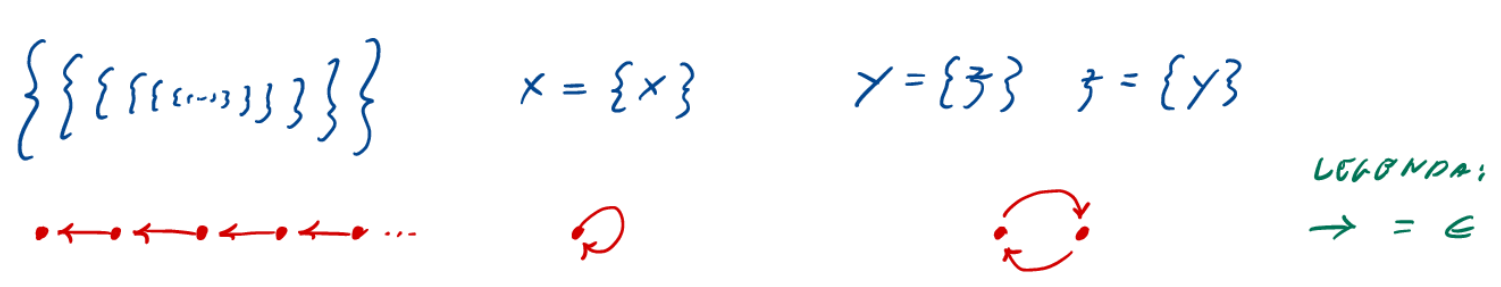
\includegraphics[width = 11.5cm]{immagini/mostri.png}
\end{figure}

Desideriamo dimostrare, intanto, che, a patto che gli assiomi della teoria degli insiemi non si contraddicano - nel qual caso dimostrerebbero qualunque cosa - essi NON dimostrano l'esistenza di insiemi del genere.\\
\textbf{\underline{Startegia}}: costruiamo un universo insiemistico $V_*$, che è una classe propria, al cui interno gli assiomi sono veri, e che, tuttavia, non contiene quella robaccia.

\begin{definition}[Gerarchia di \href{https://en.wikipedia.org/wiki/John_von_Neumann}{\textcolor{purple}{Von Neumann}}]
	Costruiamo per ricorsione transfinita la \vocab{gerarchia di Von Neumann} come segue:
	\begin{align*}
		&V_0 = \emptyset \\
		&V_{s(\alpha)} = \ps(V_\alpha) \\
		&V_\lambda = \bigcup\{V_\alpha | \alpha < \lambda\} \; \text{per $\lambda$ limite}
	\end{align*}
	La classe $V_*$ è l'unione degli insiemi $V_\alpha$, formalmente:
	\[ x \in V_* \Mydef \exists \alpha \in \Ord \; x \in V_\alpha
		\]
	(dove $V_*$ è una classe perché l'abbiamo definita come la formula al RHS).
\end{definition}

\begin{lemma}[$V_\alpha$ è transitivo]
	$\forall \alpha \in \Ord$ $V_\alpha$ è un insieme transitivo.
\end{lemma}

\begin{proof}
	Procediamo per induzione transfinita.
	\begin{itemize}
		\item[$\boxed{\text{caso $V_0$}}$] Immediato perché $\emptyset$ è un insieme transitivo a vuoto.
		\item[$\boxed{\text{caso successore}}$] Supponiamo che $V_\alpha$ sia un insieme transitivo e dimostriamo che
		anche $V_{s(\alpha)}$ lo è. Dato $x \in V_{s(\alpha)}$ vogliamo arrivare a dire che $x \subseteq V_{s(\alpha)}$ (o equivalentemente
		che $\forall y \in x \; y \in V_{s(\alpha)}$). Per farlo ci basta osservare che:
		\[ x \in V_{s(\alpha)} = \ps(V_\alpha) \implies x \subseteq V_\alpha
			\]
		ora, poiché $V_\alpha$ è transitivo per ipotesi induttiva, tutti gli elementi di $x$ sono a loro volta sottoinsiemi di $V_\alpha$ [cioè essendo elementi di un sottoinsieme sono in primis elementi di $V_\alpha$, poi per la transitività
		di quest'ultimo sappiamo che tutti gli elementi sono sottoinsiemi]\footnote{Attenzione al fatto che transitivo non dice che i sottoinsiemi sono necessariamente elementi, quindi $x$ non è detto sia un elemento di $V_\alpha$, ma è un sottoinsieme
		di $V_\alpha$ e questo ci basta.}, ovvero $\forall y \in x \; y \subseteq V_\alpha \implies \forall y \in x \; y \in \ps(V_\alpha) = V_{s(\alpha)}$, pertanto è verificata la definizione di transitività in $V_{s(\alpha)}$.
		\item[$\boxed{\text{caso limite}}$] Assumiamo per ipotesi induttiva che $V_\alpha$ sia transitivo per ogni $\alpha < \lambda$. Per definizione:
		\[ x \in V_\lambda \implies x \in V_\alpha
			\]
		per qualche $\alpha < \lambda$, ma allora per ipotesi induttiva $x \subseteq V_\alpha \subseteq V_\lambda$ [la seconda uguaglianza è la definizione nel caso limite].
	\end{itemize}
\end{proof}

\begin{corollary}[$V_*$ è una classe transitiva]
	$V_*$ è una \vocab{classe transitiva}, ossia $\forall x \in V_* \; x \subseteq V_*$.
\end{corollary}

\begin{proof}
	Se $x \in V_*$, allora per definizione $x \in V_\alpha$ per qualche $\alpha \in \Ord$, quindi per la proposizione sopra $x \subseteq V_\alpha$, ovvero $x$ è un insieme di cose che soddisfano il predicato che definisce $V_*$, quindi $x \subseteq V_*$.
\end{proof}

\begin{lemma}[``Ordinamento'' di $V_*$]
	$\forall \alpha, \beta \in \Ord \; \alpha < \beta \rightarrow V_\alpha \subseteq V_\beta$.
\end{lemma}

\begin{proof}
	Procediamo per induzione transfinita su $\beta$.
	\begin{itemize}
		\item[$\boxed{\text{caso $\beta = 0$}}$] Vero a vuoto.
		\item[$\boxed{\text{caso successore}}$] Dobbiamo dimostrare che $\forall \alpha < s(\beta) \; V_\alpha \subseteq V_{s(\beta)}$, e abbiamo per ipotesi induttiva $\forall \alpha < \beta \; V_\alpha \subseteq V_\beta$.
		Siccome $\alpha < s(\beta) \leftrightarrow \alpha \leq \beta$, si danno due casi, e $\alpha = \beta$ è banalmente vero, dunque abbiamo $\alpha < \beta$, quindi per ipotesi induttiva $V_\alpha \subseteq V_\beta$.\\
		Per la definizione ricorsiva si ha $V_\alpha \subseteq V_\beta \implies V_\alpha \in \ps(V_\beta) = V_{s(\beta)}$, ma, per la transitività di quest'ultimo, si ottiene che $V_\alpha \subseteq V_{s(\beta)}$.
		\item[$\boxed{\text{caso limite}}$] Abbiamo per ipotesi che $\forall \alpha < \beta < \lambda \; V_\alpha \subseteq V_\beta$, e vogliamo dimostrare che $\forall \alpha < \lambda \; V_\alpha \subseteq V_\beta$. Questo segue facilmente dall'ipotesi e dalla definizione,
		infatti, $V_\lambda = \bigcup\{V_\gamma | \gamma < \lambda\}$, ciò significa che $V_\beta \subseteq V_\lambda$ per ogni $\beta < \lambda$, unendo ciò all'ipotesi si ottiene la tesi, $\forall \alpha < \beta < \lambda \; V_\alpha \overset{\text{Hp. indutt.}}{\subseteq} V_\beta \overset{\text{def. $V_\lambda$}}{\subseteq} V_\lambda \implies \forall \alpha < \lambda\; V_\alpha \subseteq V_\lambda$.
		\footnote{In realtà si poteva concludere anche senza usare l'ipotesi induttiva, in quanto $\alpha < \lambda \implies V_\alpha \subseteq \bigcup{V_\gamma | \gamma < \lambda} = V_\lambda \implies V_\alpha \subseteq V_\lambda$.}
	\end{itemize}
\end{proof}

\begin{lemma}[Ogni ordinale è contenuto nella sua immagine in $V_*$]
	$\forall \alpha \in \Ord \; \alpha \subseteq V_\alpha$.
\end{lemma}

\begin{proof}
	Come al solito per induzione transfinita.
	\begin{itemize}
		\item[$\boxed{\text{caso $0$}}$] $0 \subseteq V_0 = \emptyset$, vera [perché scrivendo estesamente la formula insiemistica si ha una premessa falsa].
		\item[$\boxed{\text{caso successore}}$] Supponiamo che $\alpha \subseteq V_\alpha$ e dimostriamo che $s(\alpha) \subseteq V_{s(\alpha)}$. Osserviamo che dall'ipotesi si ha:
		\[ \alpha \subseteq V_\alpha \implies \alpha \in \ps(V_\alpha) = V_{s(\alpha)} \overset{\text{transitività}}{\implies} \alpha \subseteq V_{s(\alpha)}
			\]
		inoltre $\alpha \in V_{s(\alpha)}$ implica che $\{\alpha\} \subseteq V_{s(\alpha)}$ (se c'è come elemento, allora il suo singoletto è un suo sottoinsieme). Si conclude dunque: $s(\alpha) = \underbrace{\alpha}_{\subseteq V_{s(\alpha)}} \cup \underbrace{\{\alpha\}}_{\subseteq V_{s(\alpha)}} \subseteq V_{s(\alpha)}$.
		\item[$\boxed{\text{caso limite}}$] Per ipotesi induttiva abbiamo che $\alpha < \lambda \rightarrow \alpha \subseteq V_\alpha$, ma allora $\bigcup\{\alpha | \alpha < \lambda\} \subseteq \bigcup\{V_\alpha | \alpha < \lambda\}$ [perché abbiamo per ipotesi che ogni elemento dell'insieme al LHS è contenuto in un elemento dell'insieme al RHS, 
		quindi, prendere l'unione genera un insieme che contiene necessariamente almeno tutti gli elementi dell'altro insieme], da cui:
		\[ \lambda = \bigcup\{\alpha | \alpha < \lambda\} \;\textcolor{red}{\subseteq}\; \bigcup\{V_\alpha | \alpha < \lambda\} = V_\lambda
			\]
	\end{itemize}
\end{proof}

\subsection{Formule relativizzate ad una classe}

\begin{definition}[Relativizzazione a $V_*$]
	Data una formula insiemistica, la possiamo \vocab{relativizzare a $V_*$} rimpiazzando i quantificatori [non limitati] $\exists \square$ e $\forall \square$ rispettivamente con $\exists \square \in V_*$ e $\forall \square \in V_*$.
\end{definition}

\begin{example}[Relativizzazione di una formula a $V_*$]
	Supponiamo di voler relativizzare a $V_*$ la formula:
	\[ \varphi \equiv \exists x \; \forall y \in x \; \exists z \in y \; z \cap x = \emptyset
		\]
	Dobbiamo intanto ricondurla al linguaggio della teoria degli insiemi puro, ovvero dobbiamo rimuovere gradualmente tutte le abbreviazioni:\footnote{Typo di Mamino alla fine della terza riga, mette $t \in y$ anziché $t \in x$.}
	\begin{align*}
		& \exists x \; \forall y \in x \; \exists z \in y \; z \cap x = \emptyset \\
		& \exists x \; \forall y (y \in x \rightarrow \exists z (z \in y \land \neg \exists t (t \in z \cap x))) \\
		& \exists x \; \forall y (y \in x \rightarrow \exists z (z \in y \land \neg \exists t (t \in z \land t \in x)))
	\end{align*}
	A questo punto rimpiazziamo meccanicamente tutti i quantificatori con quantificatori limitati a $V_*$:
	\begin{align*}
		& \exists x \; \forall y (y \in x \rightarrow \exists z (z \in y \land \neg \exists t (t \in z \land t \in x))) \\
		& \exists x\in V_* \; \forall y \in V_* (y \in x \rightarrow \exists z \in V_* (z \in y \land \neg \exists t \in V_* (t \in z \land t \in x)))
	\end{align*}
	Questa nuova formula, \textcolor{MidnightBlue}{$\varphi$ relativizzata a $V_*$}, come è scritta qui sopra, non è espressa nel linguaggio della teoria degli insiemi puro, per via dei quantificatori limitati $\exists \square \in V_*$ e $\forall \square \in V_*$,
	tuttavia, se volessimo, potremmo semplicemente rimpiazzare questi quantificatori con le rispettive definizioni e ottenere così una formula insiemistica pura relativizzata a $V_*$.
\end{example}

\begin{theorem}[Gli assiomi 1-9 relativizzati sono veri in $V_*$]
	Valgono gli assiomi 1-9 della teoria degli insiemi relativizzati a $V_*$.
\end{theorem}

\begin{proof}
	Verifichiamo che valgono uno per uno gli assiomi 1-9 relativizzati in $V_*$, sfruttandone la definizione.
	\begin{enumerate}[(1)]
		\item \textbf{\underline{Vuoto}}: \textcolor{purple}{$\exists x \in V_* \; \forall y \in V_* \; y \not \in x$} \\
		Basta prendere come $x = \emptyset \in V_1 = \ps(V_0) = \ps(\emptyset) = \{\emptyset\}$, dunque $\emptyset \in V_*$, e tale insieme rispetta la proprietà richiesta perché la rispettava in $V$.
		\item \textbf{\underline{Estensionalità}}: \textcolor{purple}{$\forall a,b \in V_* (a = b \leftrightarrow \forall x \in V_* (x \in a \leftrightarrow x \in b))$} \\
		Fissati $a,b \in V_*$ osserviamo che, per transitività, i loro elementi sono anch'essi elementi di $V_*$, quindi $x \in a$ o $x \in b$ implicano $x \in V_*$, per cui si ha:
		\[ \forall x (x \in a \leftrightarrow x \in b) \leftrightarrow \forall x (x \in V_* \land (x \in a \leftrightarrow x \in b) \lor x \not \in V_* \land (x \in a \leftrightarrow x \in b))
			\] 
		ora il secondo elemento dell'OR è sempre falso per quanto detto prima, dunque possiamo escluderlo dall'equivalenza, e ciò ci lascia $\forall x \in V_* (x \in a \leftrightarrow x \in b)$.
		Dunque, per estensionalità, abbiamo l'equivalenza con $a = b$.
		\item \textbf{\underline{Separazione}}: \textcolor{purple}{$\forall A \in V_* \; \exists B \in V_* \; \forall x \in V_* \; x \in B \leftrightarrow (x \in A \land \varphi(x))$} \\
		Sia $A \in V_*$, ovvero $A \in V_\alpha$, per qualche $\alpha$, allora per separazione esiste l'insieme $B :=\{x \in A | x \in V_* \land \varphi(x)\}$. Siccome $B \subseteq A \in V_\alpha$, e $A \subseteq V_\alpha$ per transitività, si ha $B \subseteq V_\alpha \implies B \in V_{\alpha + 1}$, per cui per definizione $B \in V_*$.
		\item \textbf{\underline{Paio}}: \textcolor{purple}{$\forall a,b \in V_* \; \exists B \in V_* \; \forall x \in V_* \; x \in B \leftrightarrow (x = a \lor x = b)$} \\
		Se $a \in V_\alpha$ e $b \in V_\beta$, e, WLOG possiamo assumere $\alpha \leq \beta$, allora $\alpha, \beta \in V_\beta$, da cui necessariamente il paio, che esiste per l'assioma non relativizzato, è nelle parti di $V_\beta$, $\{a,b\} \in \ps(V_\beta) = V_{\beta + 1}$, in questo modo, per definizione si ottiene che $\{a,b\} \in V_*$.
		\item \textbf{\underline{Unione}}: \textcolor{purple}{$\forall A \in V_* \; \exists B \in V_* \; \forall x \in V_* \; x \in B \leftrightarrow \exists y \in A \; x \in y$} \\
		Sia $A \in V_\alpha$, per qualche ordinale $\alpha$, per transitività, $A \subseteq V_\alpha$, ciò significa che $\bigcup A$, che esiste per unione non relativizzata, ed è l'insieme degli elementi degli elementi di $A \subseteq V_\alpha$, è a sua volta contenuto in $V_\alpha$ (perché gli elementi degli elementi di $A$ per transitività sono a loro volta elementi di $V_\alpha$), dunque
		$\bigcup A \subseteq V_\alpha\footnote{Osserviamo che in generale $A \subseteq B \implies \bigcup A \subseteq B \iff B$ è transitivo (infatti in questo caso gli elementi di $A$ sono sottoinsiemi a loro volta di $B$, per cui la loro unione è contenuta in $B$).} \implies \bigcup A \in \ps(V_\alpha) = V_{\alpha+1}$, e quindi come prima, per definizione si conclude che $\bigcup A \in V_*$.
		\item \textbf{\underline{Parti}}: \textcolor{purple}{$\forall A \in V_* \; \exists B \in V_* \; \forall x \in V_* \; x \in B \leftrightarrow x \subseteq B$} \\
		Sia $A \in V_\alpha$, quindi per transitività $A \subseteq V_{\alpha}$, allora vale che $\ps(A) \subseteq \ps(V_\alpha) = V_{\alpha + 1}$, dove le parti esistono per l'assioma non relativizzato, quindi $\ps(A) \in \ps(V_{\alpha + 1}) = V_{\alpha + 2}$, per cui $\ps(A) \in V_*$.
		\item \textbf{\underline{Infinito}}: \textcolor{purple}{$\exists X \in V_* \; \emptyset \in X \land \forall y \in V_* \; y \in X \rightarrow y \cup \{y\} \in X$} \\
		Ci basta prendere $X = \omega \in V_{\omega + 1}$, infatti sappiamo che $\omega \subseteq V_\omega$, per quanto visto prima, quindi $\omega \in V_{\omega + 1}$, da cui $\omega \in V_*$, e naturalmente $\omega$ esiste per il corrispondente assioma non relativizzato.
		\item \textbf{\underline{Rimpiazzamento}}: \textcolor{purple}{$F : V_* \rightarrow V_*$ funzione classe e $X \in V_* \rightarrow F[X] \in V_*$} \\
		Se $X \in V_\alpha$, per transitività, $a \in X \rightarrow a \in V_\alpha$, quindi $F(a)$ è ben definito (perché $a \in V_*$) ed ha senso considerare $F[X]$, inoltre $F(a) \in V_*$ (perché $F$ va da $V_*$ a $V_*$). Sia $\alpha_a$ il minimo ordinale per cui $F(a) \in V_{\alpha_a}$
		e sia $\beta := \sup \{\alpha_a | a \in X\}$\footnote{Per essere più precisi stiamo considerando $\sup\{\rank(a) + 1|a \in X\}$, e quindi il sup esiste perché $\{\rank(a) + 1 | a \in X\}$ è effettivamente un insieme di ordinali, per rimpiazzamento (è l'immagine della funzione classe $G(a) = \rank(a) + 1$).}. Allora $F(a) \in V_{\beta}$, $\forall a \in X$, per cui $F[X] \subseteq V_\beta \implies F[X] \in V_{\beta + 1}$, dunque per definizione $F[X] \in V_*$.
		\item \textbf{\underline{Scelta}}: \textcolor{purple}{$\forall X \in V_* (\forall y \in X \; y \ne \emptyset)\footnote{Cioè se $\emptyset \not \in X$.} \rightarrow \exists f \in V_*$ funzione di scelta su $X$} \\
		Sia $f$ una funzione di scelta su $X \in V_\alpha$, che esiste per AC, sappiamo che $f \in {}^X\bigcup X$, cioè $f \in \ps\left(X \times \bigcup X\right)$. Ricordando che $X \times \bigcup X \subseteq \ps(\ps(X \cup \bigcup X))$ e che $X \subseteq V_\alpha$ (che vale per transitività) implica $\bigcup X \subseteq V_\alpha$, abbiamo:
		\[ X \cup \bigcup X \subseteq V_\alpha \implies f \in \ps\left(\ps\left(\ps\left(X \cup \bigcup X\right)\right)\right) \subseteq \ps(\ps(\ps(V_\alpha))) = V_{\alpha + 3}
			\]
		e quindi si conclude che $f \in V_*$, per definizione di quest'ultima.
	\end{enumerate}
\end{proof}

\begin{remark}[Ogni $x \in V_*$ è contenuto un insieme dato da un ordinale successore]
	Dato $x \in V_*$ esiste il minimo $\alpha$ tale che $x \in V_\alpha$ (la classe degli ordinali è ben ordinata), e questo è necessariamente un ordinale successore, perché se $x \in V_\lambda = \bigcup\{V_\alpha | \alpha < \lambda\}$, allora [per definizione di unione] $x \in V_\alpha$
	per qualche $\alpha < \lambda$, e quindi sarà in un ordinale successore. Possiamo quindi dare la definizione seguente.
\end{remark}

\begin{definition}[Rango in $V_*$]
	Dato $x \in V_*$, detto \textcolor{red}{$\alpha$ il minimo} ordinale [successore per l'osservazione] per cui $x \in V_\alpha$, il \vocab{rango} di $x$, $\rank(x)$, è definito da $\alpha = \rank(x) + 1$\footnote{Cioè il rango di un elemento
	è il predecessore del minimo ordinale per cui $x \in V_\alpha$.}. Ossia:
	\[ x \in V_\alpha \leftrightarrow \rank(x) < \alpha
		\]
	e tale definizione è ben posta per l'osservazione precedente.
\end{definition}

\begin{lemma}[Disuguaglianza tra ranghi]
	Se $x \in y \in V_*$, allora $\rank(x) < \rank(y)$.
\end{lemma}

\begin{proof}
	Per definizione di rango $y \in V_{s(\rank(y))} = \ps(V_{\rank(y)})$, quindi $y \subseteq V_{\rank(y)}$, di conseguenza, l'ipotesi $x \in y$ ci dice che $x \in V_{\rank(y)}$, per cui si ha che $\rank(x) < \rank(y)$.
\end{proof}

\begin{definition}[Classi ben fondate]
	Diciamo che una classe $C$ è \vocab{ben fondata} se per ogni insieme $S$ di elementi di $C$, $S$ contiene un $x$ \vocab{minimale per appartenenza} (\vocab{$\epsilon$-minimale}\footnote{\;``epsilon-minimale''.}),
	ossia tale che $x \cap S = \emptyset$.
\end{definition}

\begin{proposition}[Caratterizzazione classi ben fondate]
	La classe $C$ è ben fondata se e solo se \textcolor{red}{NON} esiste una famiglia $\{x_i\}_{i \in \omega}$ di elementi di $C$ tale che:
	\[ \forall i \in \omega \; x_{i+1}\in x_i
		\]
\end{proposition}

\textcolor{MidnightBlue}{Ossia non esiste una catena infinita discendente per appartenenza:}
\[ x_0 \ni x_1 \ni x_2 \ni \ldots
	\]

\begin{proof}
	Se $\{x_i\}_{i \in \omega}$ è una catena infinita discendente, allora $\{x_i | i \in \omega\}$ non ha un elemento $\epsilon$-minimale, perché per l'appartenenza infinita discendente qualsiasi elemento dell'insieme ha intersezione non vuota con quest'ultimo.\footnote{Questa è la contronominale di $\implies$, che quindi è fatta.}\\
	D'altro canto, se $S$ non ha un elemento $\epsilon$-minimale, fissata una funzione di scelta $f$ su $S$, possiamo definire una catena discendente per ricorsione numerabile. Fissiamo $\ol x \in S$ e definiamo:
	\[ x_0 = \ol x \qquad x_{n+1} = f(\{y \in S | y \in x_n\}) = f(S \cap x_n)
		\]
	dove l'insieme a cui è applicata $f$ è non vuoto, altrimenti $x_n$ sarebbe $\epsilon$-minimale, che è contro l'ipotesi.\footnote{Questa è la contronominale della $\Longleftarrow$.}
\end{proof}

Per questa caratterizzazione una classe \textcolor{purple}{transitiva}\footnote{Typo o forse no di Mamino, in ogni caso il discorso successivo non richiede la transitività, in particolare, affinché una classe non abbia mostri basta solo che sia ben fondata.} ben fondata non può quindi contenere mostri. Infatti, i mostri del primo tipo generano catene infinite discendenti per appartenenza, ed abbiamo visto che avere una classe ben fondata è equivalente al fatto che tali catene non esistano.
I mostri del secondo e terzo tipo, si riconduco, sfruttando la transitività a mostri del primi tipo, e pertanto in una classe ben fondata non esistono, come segue: dato ad esempio $x = \{x\}$, si ha che $x \in x$, ma $x = \{x\}$, cioè $\{x\} \in x \implies x \in \underbrace{\{x\}}_{= x} \in x$, e continuando in questo modo abbiamo la catena infinita discendente per appartenenza:
\[ x \ni x \ni x \ni x \ni \ldots
	\]
Dati invece $y = \{z\}$ e $z = \{y\}$ si ha che $z \in y$, ma per definizione di $z$, $y \in z$, e ripetendo questo all'infinito si ottiene:
\[  y \ni z \ni y \ni z \ni \ldots
	\]
[o anche una catena che parte da $z$], e quindi non esistono.

\begin{proposition}[$V_*$ è ben fondata]
	La classe (transitiva) $V_*$ è ben fondata.
\end{proposition}

\begin{proof}
	Dato un insieme $S$ di elementi di $V_*$, consideriamo $x \in S$ di rango minimo (cioè stiamo considerando un elemento di $S$ di rango $\min(\rank[S])$). Osserviamo che $x$ è un elemento $\epsilon$-minimale per $S$.
	Infatti, se $x \cap S \ne \emptyset$, cioè se esistesse $y \in x \cap S = \{z \in S | z \in x\}$, allora, per il lemma sul rango, essendo $y \in x$ si avrebbe $\rank(y) < \rank(x)$, ma in tal caso avremmo un elemento di $S$ con rango minore di $x$, e ciò è assurdo perché contro la minimalità di $\rank(x)$.
	Di conseguenza $x \cap S = \emptyset$.
\end{proof}

\begin{theorem}[Gli assiomi 1-9 non implicano che $V$ non sia ben fondato]
	Se gli assiomi della teoria degli insiemi sono coerenti\footnote{In caso contrario dimostrerebbero qualsiasi cosa.}, essi non dimostrano l'esistenza di una catena infinita discendente per appartenenza.\footnote{Ma non la escludono neanche, per questo abbiamo bisogno di aggiungere alla teoria un assioma apposta che ce lo assicuri.}
\end{theorem}

\begin{proof}
	Supponiamo di poter dimostrare che tale catena esiste. Allora, siccome gli assiomi valgono anche relativizzati a $V_*$, potremmo riportare l'intera dimostrazione ad una versione relativizzata, e ottenere così una catena infinita discendente per appartenenza in $V_*$,
	ma ciò è assurdo perché abbiamo dimostrato che $V_*$ è una classe ben fondata. Pertanto gli assiomi 1-9 non ci permettono di dimostrare che un tale oggetto esiste nella nostra teoria.
\end{proof}

\subsection{Assioma di buona fondazione}
A questo punto giustificati, se lo desideriamo, ad assumere che i mostri non esistano. Potremmo, per esempio, fare la cosa codarda ed assumere che la classe di tutti gli insiemi $V$ coincida con $V_*$:
\[ V = V_*
	\]
I codardi, però, non fanno mai le cose troppo apertamente, quindi assumiamo quest'altro enunciato equivalente.\footnote{In realtà assumendo buona fondazione abbiamo già risolto il problema della presenza di mostri senza necessità di dimostrare che $V = V_*$, tuttavia lo facciamo comunque perché ciò ci dà ulteriori informazioni su $V$.
In particolare avremo dimostrato che la classe di tutti gli insiemi coincide proprio con la gerarchia di Von Neumann, e ciò, oltre alla transitività ed a tutte le informazioni che conosciamo su $V_*$, ci dice anche che pensare alla classe di tutti gli insiemi organizzata come nella gerarchia è corretto (non è detto tuttavia che sia l'unico modo di pensare a $V$).}

\begin{axiom}[Assioma di buona fondazione]
	\label{ax10}
	La classe di tutti gli insiemi è ben fondata.
	\[ \forall S \ne \emptyset \; \exists x \in S \; x \cap S = \emptyset\,\footnote{Cioè ogni insieme ha un elemento $\epsilon$-minimale.}
		\]
\end{axiom}

\pagebreak
\subsection{\texorpdfstring{Principio di $\epsilon$-induzione}{Principio di epsilon-induzione}}

Per dimostrare che $V = V_*$ usando la buona fondazione, è comodo fare leva sul \vocab{principio di $\epsilon$-induzione} (epsilon-induzione).

\begin{theorem}[Principio di $\epsilon$-induzione]
	Se una classe $C$ soddisfa:
	\[ \forall S (\forall x \in S \; x \in X) \rightarrow S \in C
		\]
	Allora $C = V$, ossia $\forall S \; S \in C$.\footnote{Stiamo dicendo che, se  supponiamo che tutti gli elementi di tutti gli
	insiemi soddisfano il predicato che definisce $C$, e questa cosa ci dice che allora anche $S$ stesso soddisfa tale predicato (da qui la
	nomenclatura con la $\epsilon$, cioè dal fatto che il soddisfare una certa proprietà \textbf{passi dagli elementi a tutto l'insieme}), abbiamo che $C$ è proprio la classe di tutti gli insiemi $V$.}
\end{theorem}

La dimostrazione di questo enunciato richiede \hyperref[ax10]{buona fondazione}. Prima, però, enunciamo una proposizione che non la richiede.

\begin{proposition}[Esistenza della chiusura transitiva]
	Dato un insieme $X$ esiste più piccolo insieme transitivo $\tc(X)$ tale che $X \subseteq \tc(X)$, e prende il nome di \vocab{chiusura transitiva}.
\end{proposition}

\begin{proof}
	Costruiamo la successione $(X_n)_{n \in \omega}$ in questo modo:
	\[ X_0 = X \qquad X_{n+1} = \bigcup X_n
		\]
	Si verifica immediatamente che per definizione:
	\[ \tc(X) = \bigcup\{X_n | n \in \omega\}
		\]
	perché contiene $X = X_0 \in (X_n)_{n \in \omega}$ e tutti i suoi elementi sono anche sottoinsiemi per costruzione.
\end{proof}

Dimostriamo ora il principio di $\epsilon$-induzione.

\begin{proof}
	Procediamo per assurdo e supponiamo che si abbia $S \not \in C$. Sia:
	\[ S' := \{x \in \tc(\{S\}) | x \not \in C\} \,\footnote{Stiamo mettendo $\{S\}$ anziché $S$, in modo che $S \in \tc(\{S\})$, cosa che nel primo caso non sarebbe avvenuta.}
		\]
	Per assurdo abbiamo detto che $S \not \in C$, e questo, per la definizione di chiusura transitiva, ci assicura che $S \in S'$, che quindi è non vuoto. Per \hyperref[ax10]{buona fondazione} esiste $x \in S'$ tale che $\forall y \in x \; y \not \in S'$ [cioè tale che $x \cap S' = \emptyset$].
	Abbiamo quindi per costruzione che $x \in S' \iff x \not \in C \land x \in \tc(\{S\})$, ma la seconda cosa equivale a $x \subseteq \tc(\{S\})$, cioè $\forall y \in x \; y \in \tc(\{S\})$. Avendo preso $x$ $\epsilon$-minimale con buona fondazione, dovendo essere l'intersezione vuota, vogliamo che tutti gli elementi di $x$
	non stiano in $S'$, e visto che abbiamo appena verificato che stanno nella chiusura transitiva, l'unica possibilità è che soddisfino $C$, cioè $\forall y \in x \; y \in C$.
	Ma, per ipotesi induttiva, questa cosa implica che $x \in C$, ma avevamo che $x \in S'$, quindi $x \not \in C$, abbiamo ottenuto quindi un assurdo.
\end{proof}

\begin{proposition}[$V = V_*$]
	$\forall x \; \exists \alpha \in \Ord \; x \in V_\alpha$.
\end{proposition}

\begin{proof}
	Per $\epsilon$-induzione, ci basta dire che, fissato un insieme $S$, se [ipotesi induttiva] $\forall x \in S \; x \in V_*$, allora [passo induttivo] $S \in V_*$. Consideriamo:
	\[ \alpha := \sup\{\rank(x) + 1 | x \in S\}
		\]
	cioè l'ordinale che corrisponde all'insieme più grande, che contiene tutti gli elementi. Per ogni $x \in S$ abbiamo quindi che $x \in V_{\rank(x) + 1} \subseteq V_{\alpha}$ (cioè ognuno è contenuto nel suo, e sono tutti contenuti da $V_\alpha$), questa cosa [è una mezza freccia di estensionalità],
	e dice che $S\subseteq V_\alpha$, quindi $S \in \ps(V_\alpha) = V_{\alpha + 1} \implies S \in V_*$. Quindi per $\epsilon$-induzione $V = V_*$.
\end{proof}

\begin{corollary}[$V$ è transitivo e tutti i suoi insiemi sono costruibili in ZFC]
	Non esistono catene infinite discendenti per appartenenza.
\end{corollary}

\begin{proof}
	Avendo dimostrato che $V = V_*$, sappiamo che $V$ è una classe transitiva e ben fondata, quindi non possono esistere al suo interno dei mostri. La buona fondatezza in realtà l'avevamo già gratis assumendo \hyperref[ax10]{buona fondazione}, e di conseguenza i mostri non vi erano già, il motivo principale per cui abbiamo dimostrato l'uguaglianza è 
	dire che $V$ è anche transitivo e che la classe di tutti gli insiemi costruibili con gli assiomi 1-9, ossia $V_*$, coincide proprio con la classe di tutti gli insiemi [esistenti] $V$ (per l'assioma 10).
\end{proof}

\vfill
\begin{figure}[b]
	\centering
	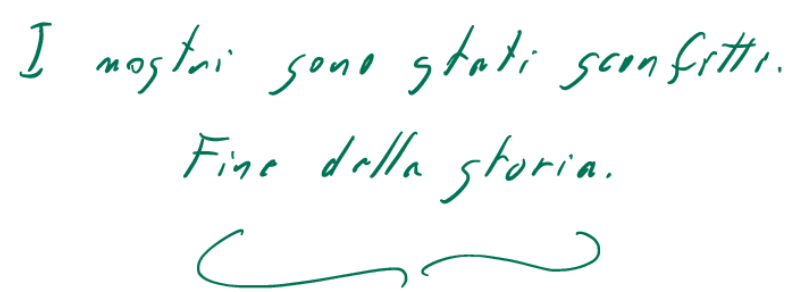
\includegraphics[width = 7.0cm]{immagini/mostri_sconfitti.png}
\end{figure}

\pagebreak

\subsection*{Esercizi}

\begin{exercise}[$|V_{\omega + \alpha}| = \beth_\alpha$]
	Definiamo $\beth_0\footnote{\;``beth''.} = \aleph_0$, $\beth_{\alpha + 1} = 2^{\beth_\alpha}$, $\beth_\lambda = \sup \{\beth_\alpha | \alpha < \lambda\}$, con $\lambda$ limite (questi cardinali definiti ricorsivamente si chiamano \vocab{beth numbers}).
	Dimostrare che $\forall \alpha \in \Ord \; |V_{\omega + \alpha}| = \beth_\alpha$.
\end{exercise}

\begin{lemma}[$\alpha \leq \beth_\alpha$]
	$\forall \alpha \in \Ord \; \alpha \leq \beth_\alpha$.\footnote{In realtà si può vedere come banale conseguenza del fatto che $\beth_\alpha : \Ord \to \Ord$ è una funzione classe strettamente crescente tra classi bene ordinate.}
\end{lemma}

\begin{proof}
	Per induzione transfinita.
	\begin{itemize}
		\item[$\boxed{\text{caso 0}}$] $0 \leq \beth_0 = \aleph_0$ è banalmente vero.
		\item[$\boxed{\text{caso $s(\alpha)$}}$] Supponiamo $\alpha < \beth_\alpha$ e osserviamo che questo significa $\alpha \leq s(\alpha) \leq \beth_\alpha$ (stiamo usando che $s(\alpha)$ è il più piccola ordinale maggiore o uguale a $\alpha$). Da ciò
		si conclude osservando che per Cantor $\beth_\alpha < 2^{\beth_\alpha} = \beth_{s(\alpha)}$, e mettendo assieme le disuguaglianze $s(\alpha) \leq \beth_{s(\alpha)}$.
		\item[$\boxed{\text{caso limite}}$] Per ipotesi induttiva abbiamo che $\alpha \leq \beth_\alpha$, per ogni $\alpha < \lambda$, essendo $x \mapsto \beth_x$ una funzione continua per costruzione, tale disuguaglianza passa quindi al sup, per cui si ottiene:
		\[ \lambda = \sup_{\alpha < \lambda} \alpha \leq \sup_{\alpha < \lambda} \beth_\alpha = \beth_\lambda
			\]
	\end{itemize}
\end{proof}

\begin{soln}
	Procediamo per induzione transfinita.
	\begin{itemize}
		\item[$\boxed{\text{caso 0}}$] $|V_{\omega + 0}| = |V_{\omega}|$, per una proposizione dimostrata sulla gerarchia, sappiamo che $\omega \subseteq V_{\omega} \implies \aleph_0 \leq |V_{\omega}|$, d'altra parte:
		\[ V_{\omega} = \bigcup_{\alpha \in \omega} V_{\alpha} \overset{\text{inclusione-esclusione}}{\implies} |V_\omega| \leq \sum_{\alpha \in \omega} |V_{\alpha}| = \max(|\omega|,|V_\alpha|)
			\]
		ma, $|V_\alpha| < \aleph_0$\footnote{Andrebbe dimostrato che, nel caso di ordinali finiti, si ha $|V_n| = 2^{V_n-1} \land |V_0| = 0$ (è una facile verifica per induzione numerabile), e ciò ci permette di dire $|V_n| \in \omega$, $\forall n \in \omega$.}, quindi abbiamo ottenuto $|V_\omega| \leq \aleph_0$. 
		\item[$\boxed{\text{caso $s(\alpha)$}}$] Supponiamo $|V_{\omega + \alpha}| = \beth_{\alpha}$ e osserviamo che $|V_{\omega + s(\alpha)}| = |\ps(V_{\omega + \alpha})| = 2^{|V_{\omega + \alpha}|}$, ora usando l'ipotesi induttiva si ottiene:
		\[ |V_{\omega + s(\alpha)}| = 2^{|V_{\omega + \alpha}|} \overset{\text{Hp. indutt.}}{=} 2^{\beth_\alpha} = \beth_{\alpha + 1}
			\]
		\item[$\boxed{\text{caso limite}}$] Per ipotesi induttiva abbiamo che $|V_{\omega + \alpha}| = \beth_\alpha$, per $\alpha < \lambda$, ci basta osservare che per definizione $V_{\omega + \alpha} \subseteq V_{\omega + \lambda}$, $\forall \alpha < \lambda$, dunque $|V_{\omega + \alpha}| \leq |V_{\omega + \lambda}|$,
		ovvero $|V_{\omega + \lambda}|$ è un maggiorante di $\{|V_{\omega + \alpha}| : \alpha < \lambda\}$, per cui:
		\[ \beth_\lambda = \sup_{\alpha < \lambda} \beth_{\alpha} \overset{\text{Hp. indutt.}}{=} \sup_{\alpha < \lambda} |V_{\omega + \alpha}| \leq |V_{\omega + \lambda}|
			\]
		mentre, per la disuguaglianza dall'alto, dato che $V_{\omega + \lambda} = \bigcup_{\alpha < \lambda} V_{\alpha}$, abbiamo:
		\begin{align*}
			|V_{\omega + \lambda}| \leq \sum_{\alpha < \lambda} |V_{\omega + \alpha}|
								   = \max\left(|\lambda|,\sup_{\alpha < \lambda} |V_{\omega + \alpha}|\right)
								   \overset{\text{Hp. indutt.}}{=} \max(|\lambda|,\beth_\lambda)
								   \overset{\text{lemma}}{=} \beth_\lambda
		\end{align*}
		in tal modo concludiamo anche il caso successore.
	\end{itemize}
\end{soln}

\begin{remark}
	Si noti che con un ragionamento analogo a quello fatto per il caso limite è possibile dimostrare che:
	\[ |V_\lambda| = \left\lvert \bigcup_{\alpha < \lambda} V_\alpha\right\rvert = \sup_{\alpha < \lambda} |V_\alpha|
		\]
	e analogamente (sfruttando il lemma di sopra):
	\[ |V_{\omega + \lambda}| = \left\lvert \bigcup_{\alpha < \lambda} V_{\omega + \alpha}\right\rvert = \sup_{\alpha < \lambda} |V_{\omega + \alpha}|
		\]
\end{remark}

\begin{exercise}[Caratterizzazione del rango]
	Dimostrare che vale la seguente identità: $\rank(x) = \sup\{\rank(y) + 1 | y \in x\}$.
\end{exercise}

\begin{soln}
	Abbiamo visto che $y \in x \implies \rank(y) < \rank (x)$, ed essendo ordinali vale $\rank(y) + 1 \leq \rank(x)$, per ogni $y \in x$, dunque $\rank(x)$ è un maggiorante dell'insieme $\{\rank(y) + 1 | y \in x\}$. Ci rimane da verificare che sia effettivamente il più piccolo maggiorante.
	Supponiamo che esista un ordinale $\alpha$ che sia maggiorante dell'insieme e allo stesso tempo $\alpha < \rank(x)$, da questo segue che $\forall y \in x \; y \in V_\alpha$, per cui $x \subseteq V_\alpha \implies x \in V_{\alpha + 1}$, pertanto, da definizione, $\rank(x) \leq \alpha$, che è assurdo.
\end{soln}

\begin{exercise}[$V_\omega$]
	Dimostrare che $V_\omega$ soddisfa tutti gli assiomi \underline{eccetto} l'\hyperref[ax7]{assioma dell'infinito}.
\end{exercise}

\begin{soln}
	Verifichiamo che valgono uno per uno gli assiomi 1-9\footnote{Avendo dimostrato che $V_*$ è ben fondata, in automatico lo è anche $V_\omega$, altrimenti si violerebbe il fatto che $V_*$ è ben fondata, pertanto non è necessario verificare che questo assioma valga in $V_\omega$.} relativizzati in $V_\omega$, eccetto l'assioma 7, ovvero l'assioma dell'infinito, ricordando che:
	\[ V_\omega = \bigcup_{\alpha < \omega} V_\alpha
		\]
	\begin{enumerate}[(1)]
		\item \textbf{\underline{Vuoto}}: \textcolor{purple}{$\exists x \in V_\omega \; \forall y \in V_\omega \; y \not \in x$} \\
		Basta prendere come $x = \emptyset \in V_1 = \ps(V_0) = \ps(\emptyset) = \{\emptyset\}$, tale insieme rispetta la proprietà richiesta e, poiché $\emptyset \in V_1 \in V_\omega$, per transitività [basta quella di $V_\omega$ stesso, ma la abbiamo comunque su tutto $V_*$] $\emptyset \in V_\omega$.
		\item \textbf{\underline{Estensionalità}}: \textcolor{purple}{$\forall a,b \in V_\omega (a = b \leftrightarrow \forall x \in V_\omega (x \in a \leftrightarrow x \in b))$} \\
		Fissati $a,b \in V_\omega$ osserviamo che, per transitività, i loro elementi sono anch'essi elementi di $V_\omega$, quindi $x \in a$ o $x \in b$ implicano $x \in V_\omega$, per cui si ha:
		\[ \forall x (x \in a \leftrightarrow x \in b) \leftrightarrow \forall x (x \in V_\omega \land (x \in a \leftrightarrow x \in b) \lor x \not \in V_\omega \land (x \in a \leftrightarrow x \in b))
			\] 
		ora il secondo elemento dell'OR è sempre falso per quanto detto prima, dunque possiamo escluderlo dall'equivalenza, e ciò ci lascia $\forall x \in V_\omega (x \in a \leftrightarrow x \in b)$.
		Dunque, per estensionalità, abbiamo l'equivalenza con $a = b$.
		\item \textbf{\underline{Separazione}}: \textcolor{purple}{$\forall A \in V_\omega \; \exists B \in V_\omega \; \forall x \in V_\omega \; x \in B \leftrightarrow (x \in A \land \varphi(x))$} \\
		Per separazione esiste l'insieme $B :=\{x \in A | x \in V_\omega \land \varphi(x)\}$. Per ipotesi $A \in V_\omega$, ovvero $A \in V_{\alpha}$, per qualche $\alpha$ ordinale, pertanto, si ha $B \subseteq A \in V_\alpha$, e per transitività $B \subseteq V_\alpha$, dunque $B \in V_{\alpha + 1}$, con $\alpha + 1 < \omega$ perché $\omega$ è limite, quindi otteniamo che $B \in V_\omega$.
		\item \textbf{\underline{Paio}}: \textcolor{purple}{$\forall a,b \in V_\omega \; \exists B \in V_\omega \; \forall x \in V_\omega \; x \in B \leftrightarrow (x = a \lor x = b)$} \\
		Dati $a,b \in V_\omega$, abbiamo che $a \in V_\alpha$ e $b \in V_\beta$, e, WLOG, possiamo assumere $\alpha \leq \beta$, allora $a,b \in V_\beta$, da cui necessariamente il paio, che esiste per l'assioma non relativizzato, è nelle parti di $V_\beta$, $\{a,b\} \in \ps(V_\beta) = V_{\beta+1}$, dove naturalmente $\beta + 1 < \omega$, e in questo modo, per transitività, si ottiene che $\{a,b\} \in V_\omega$.
		\item \textbf{\underline{Unione}}: \textcolor{purple}{$\forall A \in V_\omega \; \exists B \in V_\omega \; \forall x \in V_\omega \; x \in B \leftrightarrow \exists y \in A \; x \in y$} \\
		Sia $A \in V_\alpha$, per qualche ordinale $\alpha < \omega$, per transitività, $A \subseteq V_\alpha$, ciò significa che $\bigcup A$, che esiste per unione non relativizzata, ed è l'insieme degli elementi degli elementi di $A \subseteq V_\alpha$, è a sua volta contenuto in $V_\alpha$ (perché gli elementi degli elementi di $A$ per transitività sono a loro volta elementi di $V_\alpha$), dunque
		$\bigcup A \subseteq V_\alpha\footnote{Osserviamo che in generale $A \subseteq B \implies \bigcup A \subseteq B \iff B$ è transitivo.} \implies \bigcup A \in \ps(V_\alpha) = V_{\alpha+1}$, e quindi come prima, per transitività si conclude che $\bigcup A \in V_\omega$.
		\item \textbf{\underline{Parti}}: \textcolor{purple}{$\forall A \in V_\omega \; \exists B \in V_\omega \; \forall x \in V_\omega \; x \in B \leftrightarrow x \subseteq B$} \\
		Sia $A \in V_\alpha$, quindi per transitività $A \subseteq V_{\alpha}$, allora si ha $\ps(A) \subseteq \ps(V_\alpha) = V_{\alpha + 1}$, dove le parti esistono per l'assioma non relativizzato, quindi $\ps(A) \in \ps(V_{s(\alpha)}) = V_{\alpha + 2}$, per cui $\ps(A) \in V_\omega$.
		\item \textbf{\underline{Rimpiazzamento}}: \textcolor{purple}{$F : V_\omega \rightarrow V_\omega$ funzione classe e $X \in V_\omega \rightarrow F[X] \in V_\omega$} \\
		Sia $X \in V_\alpha$, per transitività, $\forall x \in X \to x \in V_\alpha$, cioè $X \subseteq V_\alpha$, dunque è ben definita $F[X]$ in quanto possiamo fare $F(a)$ per ogni $a \in X$, perché, come detto, $a \in V_\alpha \in V_\omega$. A questo punto, definiamo $\alpha_a :=\min\{\gamma \in \omega | F(a) \in V_\gamma\}$ e $\beta :=\sup\{\alpha_a\}_{a \in X}$, e osserviamo che l'insieme su cui stiamo prendendo il sup è finito, in quanto $|F[X]| \leq |X| \leq |V_\alpha| = 2^{|V_{\alpha - 1}|}$\footnote{Osserviamo
		sempre che ciò esclude il caso banale, e che andrebbe dimostrato che $|V_n| = 2^{|V_{n-1}|} \land |V_0| = 0$ (è una facilissima induzione numerabile) per poter assicurare la finitezza di ciò che stiamo facendo.} (e qui stiamo usando che $\alpha \in \omega$),
		dunque ha proprio un massimo $\beta \in \omega$, per cui $F(a) \in V_\beta$, $\forall a \in X$, ovvero $F[x] \subseteq V_\beta \implies F[X] \in V_{\beta + 1}$, e per transitività $F[X] \in V_\omega$.
		\item \textbf{\underline{Scelta}}: \textcolor{purple}{$\forall X \in V_\omega (\forall y \in X \; y \ne \emptyset)\footnote{Cioè se $\emptyset \not \in X$.} \rightarrow \exists f \in V_\omega$ funzione di scelta su $X$} \\
		Sia $f$ una funzione di scelta su $X \in V_\alpha$, che esiste per AC, sappiamo che $f \in {}^X\bigcup X$, cioè $f \in \ps\left(X \times \bigcup X\right)$. Ricordando che $X \times \bigcup X \subseteq \ps(\ps(X \cup \bigcup X))$ e che $X \subseteq V_\alpha$ (che vale per transitività) implica $\bigcup X \subseteq V_\alpha$, abbiamo:
		\[ X \cup \bigcup X \subseteq V_\alpha \implies f \in \ps\left(\ps\left(\ps\left(X \cup \bigcup X\right)\right)\right) \subseteq \ps(\ps(\ps(V_\alpha))) = V_{\alpha + 3}
			\]
		naturalmente $\alpha + 3 < \omega$, quindi $V_{\alpha + 3} \in V_\omega$, e per transitività si ha che $f \in V_\omega$.
	\end{enumerate}
	Infine, non ci resta che verificare che $V_\omega$ non soddisfa l'assioma dell'infinito, in primis osserviamo che $\omega \not \in V_\omega$, in quanto $\rank(\omega) = \omega$, inoltre se esistesse un insieme induttivo $X \in V_\omega$, poiché avevamo definito $\omega$ come l'intersezione della classe di tutti gli insiemi induttivi, avremmo che $\omega \subseteq X$, e siccome $X \in V_\omega \implies X \in V_\alpha$, per $\alpha < \omega$,
	si ha che $\omega \in V_{\alpha + 1} \in V_\omega \implies \omega \in V_\omega \;\lightning$.  
\end{soln}

\begin{remark}[Esistenza di insiemi infiniti]
	L'esercizio appena risolto ha come conseguenza che l'esistenza di un insieme induttivo è indipendente dagli assiomi della ZFC ad eccezione dell'assioma dell'infinito, e ciò ci dà appunto una giustificazione all'introduzione di tale assioma. In particolare senza questo insieme non possiamo costruire $\omega$ e quindi nessun altro insieme infinito (potremmo costruire solo insiemi ereditariamente finiti usando gli altri assiomi), pertanto 
	si capisce ancora meglio perché l'assioma dell'infinito ci garantisce la possibilità di definire insiemi infiniti.
\end{remark}

\begin{exercise}[$V_{\omega + \omega}$]
	Dimostrare che $V_{\omega + \omega}$ soddisfa tutti gli assiomi \underline{eccetto} l'\hyperref[ax8]{assioma del rimpiazzamento}.
\end{exercise}

\begin{soln}
	Verifichiamo che valgono uno per uno gli assiomi 1-9\footnote{Esattamente come per $V_\omega$ non è necessario dimostrare che valga buona fondazione.} relativizzati in $V_{\omega + \omega}$, eccetto l'assioma 8, ovvero l'assioma del rimpiazzamento, ricordando che:
	\[ V_{\omega + \omega} = \bigcup_{\alpha < \omega} V_{\omega + \alpha}
		\]
	\begin{enumerate}[(1)]
		\item \textbf{\underline{Vuoto}}: \textcolor{purple}{$\exists x \in V_{\omega + \omega} \; \forall y \in V_{\omega + \omega} \; y \not \in x$} \\
		Basta prendere come $x = \emptyset \in V_1 = \ps(V_0) = \ps(\emptyset) = \{\emptyset\}$, tale insieme rispetta la proprietà richiesta e, poiché $\emptyset \in V_1 \in V_{\omega + \omega}$, per transitività [basta quella di $V_{\omega + \omega}$ stesso, ma la abbiamo comunque su tutto $V_*$] $\emptyset \in V_{\omega + \omega}$.
		\item \textbf{\underline{Estensionalità}}: \textcolor{purple}{$\forall a,b \in V_{\omega + \omega} (a = b \leftrightarrow \forall x \in V_{\omega + \omega} (x \in a \leftrightarrow x \in b))$} \\
		Fissati $a,b \in V_{\omega + \omega}$ osserviamo che, per transitività, i loro elementi sono anch'essi elementi di $V_{\omega + \omega}$, quindi $x \in a$ o $x \in b$ implicano $x \in V_{\omega + \omega}$, per cui si ha:
		\[ \forall x (x \in a \leftrightarrow x \in b) \leftrightarrow \forall x (x \in V_{\omega + \omega} \land (x \in a \leftrightarrow x \in b) \lor x \not \in V_{\omega + \omega} \land (x \in a \leftrightarrow x \in b))
			\] 
		ora il secondo elemento dell'OR è sempre falso per quanto detto prima, dunque possiamo escluderlo dall'equivalenza, e ciò ci lascia $\forall x \in V_{\omega + \omega} (x \in a \leftrightarrow x \in b)$.
		Dunque, per estensionalità, abbiamo l'equivalenza con $a = b$.
		\item \textbf{\underline{Separazione}}: \textcolor{purple}{$\forall A \in V_{\omega + \omega} \; \exists B \in V_{\omega + \omega} \; \forall x \in V_{\omega + \omega} \; x \in B \leftrightarrow (x \in A \land \varphi(x))$} \\
		Per separazione esiste l'insieme $B :=\{x \in A | x \in V_{\omega + \omega} \land \varphi(x)\}$. Per ipotesi $A \in V_{\omega + \omega}$, ovvero $A \in V_{\alpha}$, per qualche $\alpha$ ordinale, pertanto, si ha $B \subseteq A \in V_\alpha$, e per transitività $B \subseteq V_\alpha$, dunque $B \in V_{\alpha + 1}$, con $\alpha + 1 < {\omega + \omega}$ perché ${\omega + \omega}$ è limite, quindi otteniamo che $B \in V_{\omega + \omega}$.
		\item \textbf{\underline{Paio}}: \textcolor{purple}{$\forall a,b \in V_{\omega + \omega} \; \exists B \in V_{\omega + \omega} \; \forall x \in V_{\omega + \omega} \; x \in B \leftrightarrow (x = a \lor x = b)$} \\
		Dati $a,b \in V_{\omega + \omega}$, abbiamo che $a \in V_\alpha$ e $b \in V_\beta$, e, WLOG, possiamo assumere $\alpha \leq \beta$, allora $a,b \in V_\beta$, da cui necessariamente il paio, che esiste per l'assioma non relativizzato, è nelle parti di $V_\beta$, $\{a,b\} \in \ps(V_\beta) = V_{\beta+1}$, dove naturalmente $\beta + 1 < {\omega + \omega}$, e in questo modo, per transitività, si ottiene che $\{a,b\} \in V_{\omega + \omega}$.
		\item \textbf{\underline{Unione}}: \textcolor{purple}{$\forall A \in V_{\omega + \omega} \; \exists B \in V_{\omega + \omega} \; \forall x \in V_{\omega + \omega} \; x \in B \leftrightarrow \exists y \in A \; x \in y$} \\
		Sia $A \in V_\alpha$, per qualche ordinale $\alpha < \omega + \omega$, per transitività, $A \subseteq V_\alpha$, ciò significa che $\bigcup A$, che esiste per unione non relativizzata, ed è l'insieme degli elementi degli elementi di $A \subseteq V_\alpha$, è a sua volta contenuto in $V_\alpha$ (perché gli elementi degli elementi di $A$ per transitività sono a loro volta elementi di $V_\alpha$), dunque
		$\bigcup A \subseteq V_\alpha\footnote{Osserviamo che in generale $A \subseteq B \implies \bigcup A \subseteq B \iff B$ è transitivo.} \implies \bigcup A \in \ps(V_\alpha) = V_{\alpha+1}$, e quindi come prima, per transitività si conclude che $\bigcup A \in V_{\omega + \omega}$.
		\item \textbf{\underline{Parti}}: \textcolor{purple}{$\forall A \in V_{\omega + \omega} \; \exists B \in V_{\omega + \omega} \; \forall x \in V_{\omega + \omega} \; x \in B \leftrightarrow x \subseteq B$} \\
		Sia $A \in V_\alpha$, quindi per transitività $A \subseteq V_{\alpha}$, allora si ha $\ps(A) \subseteq \ps(V_\alpha) = V_{\alpha + 1}$, dove le parti esistono per l'assioma non relativizzato, quindi $\ps(A) \in \ps(V_{s(\alpha)}) = V_{\alpha + 2}$, per cui $\ps(A) \in V_{\omega + \omega}$.
		\item \textbf{\underline{Infinito}}: \textcolor{purple}{$\exists X \in V_{\omega + \omega} \; \emptyset \in X \land \forall x \in X \to x \cup \{x\} \in X$} \\
		Basta prendere $X = \omega \in V_{\omega + 1}$, con $V_{\omega + 1} \in V_{\omega + \omega}$, e per transitività $X \in V_{\omega + \omega}$.
		\item \textbf{\underline{Scelta}}: \textcolor{purple}{$\forall X \in V_{\omega + \omega} (\forall y \in X \; y \ne \emptyset)\footnote{Cioè se $\emptyset \not \in X$.} \rightarrow \exists f \in V_{\omega + \omega}$ funzione di scelta su $X$} \\
		Sia $f$ una funzione di scelta su $X \in V_\alpha$, che esiste per AC, sappiamo che $f \in {}^X\bigcup X$, cioè $f \in \ps\left(X \times \bigcup X\right)$. Ricordando che $X \times \bigcup X \subseteq \ps(\ps(X \cup \bigcup X))$ e che $X \subseteq V_\alpha$ (che vale per transitività) implica $\bigcup X \subseteq V_\alpha$, abbiamo:
		\[ X \cup \bigcup X \subseteq V_\alpha \implies f \in \ps\left(\ps\left(\ps\left(X \cup \bigcup X\right)\right)\right) \subseteq \ps(\ps(\ps(V_\alpha))) = V_{\alpha + 3}
			\]
		naturalmente $\alpha + 3 < {\omega + \omega}$, quindi $V_{\alpha + 3} \in V_{\omega + \omega}$, e per transitività si ha che $f \in V_{\omega + \omega}$.
	\end{enumerate}
	Infine, dobbiamo dimostrare che non vale l'assioma del rimpiazzamento, osserviamo in primis che l'argomento utilizzato per dimostrare la validità di questo assioma per $V_{\omega}$ qui fallisce in quanto $\beta$ non è necessariamente finito, ed in particolare potrebbe accadere che $\beta = \omega + \omega$, il che implicherebbe $F[X] \in V_{\omega + \omega + 1}$, e ciò fa fallire la dimostrazione in questo caso.
	Supponiamo per assurdo che $V_{\omega + \omega}$ soddisfi l'assioma del rimpiazzamento, allora esiste l'insieme $\omega + \omega \in V_{\omega + \omega}$, per la dimostrazione vista che ogni classe di isomorfismo ha associato un ordinale (ed in particolare ci basta prendere l'ordinale associato all'insieme di vuoto e $\omega$ in un numero finito di singoletti che abbiamo visto in un esercizio nella sezione sugli ordinali),
	ma ciò è assurdo in quanto, per la proprietà del rango di un ordinale, si ha $\rank(\omega + \omega) = \omega + \omega \implies \omega + \omega \not \in V_{\omega + \omega}$.
\end{soln}

\begin{exercise}[Rimpiazzamento $\implies \exists\, \omega + \omega$]
	Dimostrare che l'esistenza dell'ordinale $\omega + \omega$ non segue dagli assiomi della teoria degli insiemi, \underline{escluso} l'\hyperref[ax8]{assioma del rimpiazzamento}, a patto 
	che questi non si contraddicano.
\end{exercise}

\begin{soln}
	Se per assurdo l'esistenza di $\omega + \omega$ seguisse dagli assiomi della ZFC tranne rimpiazzamento, assumendo che sono coerenti (e quindi non si contraddicono, altrimenti potremmo dimostrare qualsiasi cosa),
	allora un tale ordinale esisterebbe anche in $V_{\omega + \omega}$, visto che abbiamo dimostrato che in tale insieme valgono tutti gli assiomi tranne appunto rimpiazzamento.
	Tuttavia, sappiamo che $\rank(\omega + \omega) = \omega + \omega$, quindi $\omega + \omega \not \in V_{\omega + \omega}$, pertanto ciò è assurdo. Abbiamo quindi dimostrato che l'esistenza dell'ordinale $\omega + \omega$ è indipendente dagli assiomi della ZFC, escluso il rimpiazzamento.
\end{soln}

\begin{exercise}[$V_\kappa$ - $\kappa$ fortemente inaccessibile]
	Dimostrare che, se $\kappa$ è [fortemente] inaccessibile, allora tutti gli assiomi della teoria degli insiemi valgono in $V_\kappa$.
\end{exercise}

\begin{soln}
	Ricordiamo innanzitutto che $\kappa$ fortemente inaccessibile significa che $\kappa$ è un ordinale iniziale (quindi limite) regolare, $\cof(\kappa) = \kappa$, ed è limite forte, cioè $\aleph_0 < \kappa$ e $\forall \alpha \; \aleph_\alpha < \kappa \to 2^{\aleph_\alpha} < \kappa$. Ciò significa che $\omega < \kappa \to V_\omega \in V_\kappa$.\footnote{Come al solito $V_*$ è ben fondata, dunque non è necessario verificare buona fondazione in $V_\kappa$, in quanto è già dato.}
	\begin{enumerate}[(1)]
		\item \textbf{\underline{Vuoto}}: \textcolor{purple}{$\exists x \in V_\kappa \; \forall y \in V_\kappa \; y \not \in x$} \\
		Basta prendere come $x = \emptyset \in V_1 = \ps(V_0) = \ps(\emptyset) = \{\emptyset\}$, tale insieme rispetta la proprietà richiesta e, poiché $\emptyset \in V_1 \in V_\kappa$, per transitività [basta quella di $V_\kappa$ stesso, ma la abbiamo comunque su tutto $V_*$] $\emptyset \in V_\kappa$.
		\item \textbf{\underline{Estensionalità}}: \textcolor{purple}{$\forall a,b \in V_\kappa (a = b \leftrightarrow \forall x \in V_\kappa (x \in a \leftrightarrow x \in b))$} \\
		Fissati $a,b \in V_\kappa$ osserviamo che, per transitività, i loro elementi sono anch'essi elementi di $V_\kappa$, quindi $x \in a$ o $x \in b$ implicano $x \in V_\kappa$, per cui si ha:
		\[ \forall x (x \in a \leftrightarrow x \in b) \leftrightarrow \forall x (x \in V_\kappa \land (x \in a \leftrightarrow x \in b) \lor x \not \in V_\kappa \land (x \in a \leftrightarrow x \in b))
			\] 
		ora il secondo elemento dell'OR è sempre falso per quanto detto prima, dunque possiamo escluderlo dall'equivalenza, e ciò ci lascia $\forall x \in V_\kappa (x \in a \leftrightarrow x \in b)$.
		Dunque, per estensionalità, abbiamo l'equivalenza con $a = b$.
		\item \textbf{\underline{Separazione}}: \textcolor{purple}{$\forall A \in V_\kappa \; \exists B \in V_\kappa \; \forall x \in V_\kappa \; x \in B \leftrightarrow (x \in A \land \varphi(x))$} \\
		Per separazione esiste l'insieme $B :=\{x \in A | x \in V_\kappa \land \varphi(x)\}$. Per ipotesi $A \in V_\kappa$, ovvero $A \in V_{\alpha}$, per qualche $\alpha$ ordinale, pertanto, si ha $B \subseteq A \in V_\alpha$, e per transitività $B \subseteq V_\alpha$, dunque $B \in V_{\alpha + 1}$, con $\alpha + 1 < \kappa$ perché $\kappa$ è limite, quindi otteniamo che $B \in V_\kappa$.
		\item \textbf{\underline{Paio}}: \textcolor{purple}{$\forall a,b \in V_\kappa \; \exists B \in V_\kappa \; \forall x \in V_\kappa \; x \in B \leftrightarrow (x = a \lor x = b)$} \\
		Dati $a,b \in V_\kappa$, abbiamo che $a \in V_\alpha$ e $b \in V_\beta$, e, WLOG, possiamo assumere $\alpha \leq \beta$, allora $a,b \in V_\beta$, da cui necessariamente il paio, che esiste per l'assioma non relativizzato, è nelle parti di $V_\beta$, $\{a,b\} \in \ps(V_\beta) = V_{\beta+1}$, dove naturalmente $\beta + 1 < \kappa$, e in questo modo, per transitività, si ottiene che $\{a,b\} \in V_\kappa$.
		\item \textbf{\underline{Unione}}: \textcolor{purple}{$\forall A \in V_\kappa \; \exists B \in V_\kappa \; \forall x \in V_\kappa \; x \in B \leftrightarrow \exists y \in A \; x \in y$} \\
		Sia $A \in V_\alpha$, per qualche ordinale $\alpha < \kappa$, per transitività, $A \subseteq V_\alpha$, ciò significa che $\bigcup A$, che esiste per unione non relativizzata, ed è l'insieme degli elementi degli elementi di $A \subseteq V_\alpha$, è a sua volta contenuto in $V_\alpha$ (perché gli elementi degli elementi di $A$ per transitività sono a loro volta elementi di $V_\alpha$), dunque
		$\bigcup A \subseteq V_\alpha\footnote{Osserviamo che in generale $A \subseteq B \implies \bigcup A \subseteq B \iff B$ è transitivo.} \implies \bigcup A \in \ps(V_\alpha) = V_{\alpha+1}$, e quindi come prima, per transitività si conclude che $\bigcup A \in V_\kappa$.
		\item \textbf{\underline{Parti}}: \textcolor{purple}{$\forall A \in V_\kappa \; \exists B \in V_\kappa \; \forall x \in V_\kappa \; x \in B \leftrightarrow x \subseteq B$} \\
		Sia $A \in V_\alpha$, quindi per transitività $A \subseteq V_{\alpha}$, allora si ha $\ps(A) \subseteq \ps(V_\alpha) = V_{\alpha + 1}$, dove le parti esistono per l'assioma non relativizzato, quindi $\ps(A) \in \ps(V_{s(\alpha)}) = V_{\alpha + 2}$, per cui $\ps(A) \in V_\kappa$.
		\item \textbf{\underline{Infinito}}: \textcolor{purple}{$\exists X \in V_\kappa \; \emptyset \in X \land \forall x \in X \to x \cup \{x\} \in X$} \\
		Basta prendere $X = \omega \in V_{\omega + 1}$, con $V_{\omega + 1} \in V_\kappa$, e per transitività $X \in V_\kappa$.
		\item \textbf{\underline{Scelta}}: \textcolor{purple}{$\forall X \in V_\kappa (\forall y \in X \; y \ne \emptyset)\footnote{Cioè se $\emptyset \not \in X$.} \rightarrow \exists f \in V_\kappa$ funzione di scelta su $X$} \\
		Sia $f$ una funzione di scelta su $X \in V_\alpha$, che esiste per AC, sappiamo che $f \in {}^X\bigcup X$, cioè $f \in \ps\left(X \times \bigcup X\right)$. Ricordando che $X \times \bigcup X \subseteq \ps(\ps(X \cup \bigcup X))$ e che $X \subseteq V_\alpha$ (che vale per transitività) implica $\bigcup X \subseteq V_\alpha$, abbiamo:
		\[ X \cup \bigcup X \subseteq V_\alpha \implies f \in \ps\left(\ps\left(\ps\left(X \cup \bigcup X\right)\right)\right) \subseteq \ps(\ps(\ps(V_\alpha))) = V_{\alpha + 3}
			\]
		naturalmente $\alpha + 3 < \kappa$, quindi $V_{\alpha + 3} \in V_\kappa$, e per transitività si ha che $f \in V_\kappa$.
		\item \textbf{\underline{Rimpiazzamento}}: \textcolor{purple}{$F : V_\kappa \rightarrow V_\kappa$ funzione classe e $X \in V_\kappa \rightarrow F[X] \in V_\kappa$} \\
		Sia $X \in V_\alpha$, con $\alpha < \kappa$, per transitività, $\forall x \in X \to x \in V_\alpha$, cioè $X \subseteq V_\alpha$, dunque è ben definita $F[X]$ in quanto possiamo fare $F(a)$ per ogni $a \in X$, perché, come detto, $a \in V_\alpha \in V_\kappa$, inoltre $F(a) \in V_\kappa$ per definizione di $F$. A questo punto, definiamo $\alpha_a :=\min\{\gamma \in \kappa | F(a) \in V_\gamma\footnote{Per la precisione, per definizione di $F$ e $V_\kappa$, si ha $F(a) \in V_\kappa \to F(a) \in V_\gamma$, $\gamma \in \kappa$. Dunque
		gli $\alpha_a$ sono tutti strettamente minori di $\kappa$, il problema è che potrebbe non esserlo il loro sup.}\}$ e $\beta :=\sup\{\alpha_a\}_{a \in X}$, essendo 
		$F : V_\kappa \to V_\kappa$ abbiamo che $\beta \leq \kappa$, se escludiamo che $\beta = \kappa$, allora $\beta < \kappa$, per cui, essendo $\kappa$ limite, $\beta + 1 < \kappa$ ed a questo punto abbiamo $F[X] \subseteq V_\beta \implies F[X] \in V_{\beta + 1} \in V_\kappa$ e si conclude per transitività.\\
		Ci rimane quindi da escludere che $\beta = \kappa$. Per ipotesi sappiamo che $\beta = \kappa = \cof(\kappa)$, osserviamo che $\{\alpha_a | a \in X\}$ è un sottoinsieme cofinale di $\beta$ praticamente perché $\beta$ è l'estremo superiore di questo insieme (dunque la definizione di sottoinsieme cofinale è verificata immediatamente),
		inoltre si ha $|\{\alpha_a | a \in X\}| \leq |X|$ (ci basta considerare la mappa $x \mapsto \alpha_x$ che è surgettiva\footnote{Per la precisione $X \twoheadrightarrow s[\rank[X]] : x \to \alpha_x$, dove l'insieme d'arrivo è un insieme per rimpiazzamento non relativizzato.}), a questo punto, se verifichiamo che $|X| < \kappa$ abbiamo un assurdo:
		\[ \kappa = \cof(\kappa) = \cof(\beta) \leq |X| < \kappa \; \lightning
			\]
		Per dimostrare l'ultima cosa ci basta dimostrare per induzione transfinita che $|V_\alpha| < \kappa$, $\forall \alpha < \kappa$, da cui si ha $X \subseteq V_\alpha \implies |X| \leq |V_\alpha| < \kappa$, $\alpha < \kappa$.
		\begin{itemize}
			\item[$\boxed{\text{caso 0}}$] È ovvio che $0 = |V_0| < \kappa$, in quanto $\kappa > \aleph_0$ poiché limite forte. 
			\item[$\boxed{\text{caso successore}}$] Supponiamo $|V_\alpha| < \kappa$, a questo punto $|V_{\alpha + 1}| = 2^{|V_\alpha|} < \kappa$, dove l'ultima disuguaglianza vale perché $\kappa$ è limite forte.
			\item[$\boxed{\text{caso limite}}$] Abbiamo per ipotesi $|V_\alpha| < \kappa$, per $\alpha < \lambda < \kappa$, dunque:
			\[ |V_\lambda| = \left\lvert \bigcup_{\alpha < \lambda} V_\alpha\right\rvert \leq \sum_{\alpha < \lambda} |V_\alpha| = |\lambda| \cdot \sup_{\alpha < \lambda} |V_\alpha| \leq \kappa
				\]
			ora, essendo che $|\lambda| < \kappa$ e per ipotesi induttiva $|V_\alpha| < \kappa$, con $\alpha < \kappa$, se la somma facesse $\kappa$, avremmo trovato una stima dall'alto per la cofinalità, data da $|\lambda| < \kappa$, ma $\cof(\kappa) = \kappa$, dunque ciò è assurdo, e la somma è $<\kappa$.
		\end{itemize}
	\end{enumerate}
\end{soln}

\begin{remark}[Alternativa per il rimpiazzamento in $V_\kappa$]
	Il punto chiave della dimostrazione della validità dell'assioma del rimpiazzamento in $V_\kappa$ è l'assurdo ottenuto violando il fatto che $\kappa$ sia regolare, questa cosa può essere fatta anche ragionando sulla prima definizione data di cofinalità, così da escludere che $\beta = \kappa$.\\
	Per verificare che $\beta < \kappa$ è sufficiente verificare che $|\beta| < \kappa$, essendo $\kappa$ un ordinale iniziale, e, essendo $\beta = \bigcup_{a \in X} \alpha_a$ si ha:
	\[ |\beta| \leq \sum_{a \in X} |\alpha_a| = |X| \cdot \sup_{a \in X} |\alpha_a|
		\]
	a questo punto, come nella dimostrazione sopra, sappiamo che $|X| < \kappa$, per cui, se la somma sopra fosse uguale a $\kappa$, allora il sup sarebbe uguale a $\kappa$, ma $|\alpha_a| < \kappa$, $\forall a \in X$, in quanto $a \in X$, per cui avremmo ottenuto una stima dall'alto per la cofinalità (v.1) di $\kappa$ (cioè avremmo ottenuto che $\kappa$ si può scrivere come somma di cose più piccole
	un numero di volte $< \kappa$) che è assurda in quanto $\kappa = \cof(\kappa) \leq |X| < \kappa$. Segue quindi che la somma è minore strettamente di $\kappa$, dunque $|\beta| < \kappa$.\footnote{Idea proposta da Rubens Alessio Martino.}
\end{remark}

\begin{exercise}[ZFC $\notimplies$ esiste un cardinale fortemente inaccessibile]
	Dimostrare che, se la teoria degli insiemi è coerente, allora non dimostra l'esistenza di un cardinale [fortemente] inaccessibile.
\end{exercise}

\begin{soln}
	Se per assurdo l'esistenza di un cardinale fortemente inaccessibile $\kappa$ seguisse dagli assiomi della ZFC, assumendo che sono coerenti (e quindi non si contraddicono, altrimenti potremmo dimostrare qualsiasi cosa), allora,
	per quanto dimostrato nell'esercizio precedente, l'esistenza di $\kappa$ seguirebbe anche in $V_\kappa$, avendo dimostrato che anche qui valgono tutti gli assiomi. Tuttavia ciò è assurdo in quanto $\rank(\kappa) = \kappa$ ($\kappa$ è un cardinale, dunque un ordinale iniziale, quindi vale anche per lui la proprietà del rango degli ordinali), quindi 
	$\kappa \not \in V_\kappa$, pertanto l'esistenza di un cardinale fortemente inaccessibile è indipendente dagli assiomi della ZFC.
\end{soln}

\begin{remark}[$V_\kappa$ - $\kappa$ debolmente inaccessibile]
	Si potrebbe essere tentati di dimostrare che anche nel caso di $V_\kappa$, con $\kappa$ cardinale debolmente inaccessibile siano verificati tutti gli assiomi della ZFC, ed in effetti lo sono tutti ad eccezione del rimpiazzamento. In particolare, non solo la dimostrazione fatta nel caso di $\kappa$ fortemente inaccessibile non funziona (poiché avevamo usato l'ipotesi di limite forte),
	ma si verifica addirittura che rimpiazzamento non può proprio valere in $V_\kappa$, con $\kappa$ debolmente inaccessibile.
\end{remark}

\begin{proof}
	Sia $V_{\kappa}$, con $\kappa$ cardinale debolmente inaccessibile, essendo che $\kappa$ non è limite forte, esiste almeno un cardinale $\lambda < \kappa$, tale che $2^{\lambda} \geq \kappa$. A questo punto 
	ci basta considerare l'Hartogs $H(2^{\lambda}) > 2^{\lambda}$, se valesse il rimpiazzamento si avrebbe che $H(2^{\lambda}) \in V_{\kappa}$, ma, d'altra parte, si ha:
	\[ \kappa \leq 2^{\lambda} < H(2^\lambda) \in V_{\kappa} \implies \kappa \in H(2^\lambda) \in V_{\kappa} \implies \kappa \in V_{\kappa} \; \lightning
		\]
\end{proof}

\begin{remark}
	[Esistenza di un cardinale debolmente inaccessibile in ZFC]
	L'esistenza di cardinali debolmente inaccessibili, analogamente a quella dei fortemente inaccessibili, è indipendente dalla ZFC, ma non possiamo dimostrarlo usando solo la gerarchia di Von Neumann come fatto nel caso dei fortemente inaccessibili per il motivo appena visto.
\end{remark}
\appendix
\section{Appendice}
\subsection{Cardinalità note}
In questa sezione risolviamo gli esercizi lasciati nel foglio di esercizi \cite{mamino_eti_22_23_esercizi}, proposto a metà del corso dal prof. Mamino (le note aggiunte sono quelle del prof. stesso alle soluzioni da lui proposte \cite{mamino_eti_22_23_sol_esercizi}).

\begin{exercise}[Cardinalità di base]
	Determinare le seguenti cardinalità.
\end{exercise}

\begin{itemize}
	\item \textcolor{purple}{$|$numeri irrazionali$|$ $= |\RR \setminus \QQ|$}
\end{itemize}

\begin{soln}
	(Senza AC)\\
	Poiché $\RR$ è continuo e $\QQ$ numerabile, per il \hyperref[continuo-numerabile]{lemma}, la differenza rimane continua e quindi $|\RR \setminus \QQ| = 2^{\aleph_0}$.
\end{soln}

\begin{note}[Sulla sottrazione di cardinalità]
	In sostanza $2^{\aleph_0} - \aleph_0 = 2^{\aleph_0}$, ma scrivere questa sottrazione sarebbe \textcolor{red}{SBAGLIATO}, perché, in generale, la differenza di cardinalità non è definita. Sarebbe anche \textcolor{red}{SBAGLIATO PENSARE}
	che stiamo usando il fatto che $2^{\aleph_0} + \aleph_0 = 2^{\aleph_0}$, infatti, da questa uguaglianza, \textbf{non} si deduce che se $|X| + \aleph_0 = 2^{\aleph_0}$ allora $|X| = 2^{\aleph_0}$.
	In realtà stiamo usando un \hyperref[continuo-numerabile]{lemma} visto a lezione (dimostrato senza AC):
	\[ |A| = 2^{\aleph_0} \land B \subseteq A \land |B| \leq \aleph_0 \rightarrow |A \setminus B| = 2^{\aleph_0}
 		\]
	e la soluzione cita esattamente le ipotesi del lemma.
\end{note}

\begin{itemize}
	\item \textcolor{purple}{$|$reali trascendenti$|$ $= |\RR \setminus \mathbb{A}_{\RR}|$}
\end{itemize}

\begin{soln}
	(Senza AC)\\
	Abbiamo già dimostrato che $|\mathbb A_\RR| = \aleph_0$, quindi per il \hyperref[continuo-numerabile]{lemma}, si ha $|\RR \setminus \mathbb{A}_{\RR}| = 2^{\aleph_0}$.
\end{soln}

\begin{itemize}
	\item \textcolor{purple}{$|$sottoinsiemi infiniti di $\omega|$ $= |\ps(\omega) \setminus \psf(\omega)|$}
\end{itemize}

\begin{soln}
	(Senza AC)\\
	Abbiamo dimostrato che $|\psf(\omega)| = \aleph_0$ e dal \hyperref[continuo-numerabile]{lemma} si ottiene $|\ps(\omega) \setminus \psf(\omega)| = 2^{\aleph_0}$.
\end{soln}

\begin{itemize}
	\item \textcolor{purple}{$|$sottoinsiemi finiti di $\RR|$ $= |\psf(\RR)|$}\footnote{È banale con AC, poiché lo abbiamo \hyperref[parti_finite_generale]{dimostrato in generale}, che $|\psf(\RR)| = |\RR| = 2^{\aleph_0}$.}
\end{itemize}

\textcolor{MidnightBlue}{\underline{Idea}: Va da sé che i sottoinsiemi finiti di $\RR$ sono almeno tanti quanti i reali stessi. D'altro canto, se avessimo l'assioma della scelta,
potremmo dimostrare, che, fatto per altro intuitivo, l'immagine di una funzione ha cardinalità al più pari al dominio: $|f[X]| \leq |X|$.\footnote{In realtà abbiamo dimostrato per \hyperref[disuguaglianze_senza_AC1]{esercizio} che questa cosa è vera anche senza AC nel caso in cui l'insieme sia finito, ma la dimostrazione si adatta subito al caso al più numerabile (assieme anche al fatto che le disuguaglianze di surgettività, sempre nel caso di insiemi al più numerabili, sono \hyperref[disuguaglianze_senza_AC2]{valide} anche senza AC).}
Siccome ogni insieme finito di reali è immagine di una successione di reali, considerando la funzione $f$ che manda una successione nella sua immagine avremmo $|\text{sottoinsiemi finite dei reali}| \leq |\text{successioni di reali}| = (2^{\aleph_0})^{\aleph_0} = 2^{\aleph_0}$.
Per aggirare il lemma vietato $|f[X]|\leq |X|$, possiamo lavorare al contrario, cercando una funzione iniettiva che manda i sottoinsiemi finiti di $\RR$ nella successioni.}

\begin{soln}
	È facile vedere la funzione $\RR \hookrightarrow \psf(\RR) : x \mapsto \{x\}$ è iniettiva e ci dà la disuguaglianza dal basso $2^{\aleph_0} \leq|\psf(\RR)|$. Viceversa, dato $A \in \psf(\RR)$, per definizione esiste $n \in \omega$ tale che $n = |A|$,
	quindi possiamo definire la funzione $\psf(\RR) \to {}^\omega(\RR \cup \{\spadesuit\}) : A \mapsto a_i$, dove:
	\[ a_{i} = \begin{cases}
		\min_{<_{\RR|A}}(A\setminus\Imm(a_{|i}))&\text{se $i < n$} \\
		\spadesuit &\text{se $i \geq n$}
	\end{cases}
		\]
	in tal modo si ha che $\Imm(a_{|i}) \cap \RR = A$. Quindi segue facilmente che questa mappa è iniettiva (due successioni con la stessa immagine, per la proprietà appena menzionata, danno lo stesso insieme usato in partenza) e ci dà la disuguaglianza dall'alto 
	$|\psf(\RR)| \leq |\RR \cup \{\spadesuit\}| \leq 2^{\aleph_0}$ (dove l'ultima uguaglianza è inclusione-esclusione).\footnote{Osservare che questa identica dimostrazione funziona per tutte le parti finite di un insieme in cui abbiamo un modo per scegliere un elemento da un suo sottoinsieme, mentre fallisce su $\omega$ [nonostante qui il modo di scegliere lo abbiamo] in 
	quanto qualsiasi insieme di successioni su un insieme infinito ha almeno sempre cardinalità $\aleph_0^{\aleph_0} = 2^{\aleph_0}$.}
\end{soln}

\begin{soln}
	(Soluzione alternativa buffa (idea))
	La funzione $g : \psf(\RR) \to {}^\omega\RR : X \mapsto g(X)$ definita da:
	\[ g(X) : n \mapsto \sum_{x \in X} \text e^{n \cdot x}
		\]
	è iniettiva.
\end{soln}

\begin{itemize}
	\item \textcolor{purple}{$|$sottoinsiemi infiniti di $\RR|$ $= |\ps(\RR)\setminus\psf(\RR)| = |\psinf(\RR)|$}
\end{itemize}

\begin{soln}
	(Senza AC)\\
	Ovviamente $\psinf(\RR) := \ps(\RR)\setminus\psf(\RR) \subseteq \ps(\RR) \implies |\psinf(\RR)|\leq 2^{2^{\aleph_0}}$. Viceversa (per la caratterizzazione di $(\RR,<)$ come ordine) abbiamo che $|]0,1[| = |\RR|$,
	quindi abbiamo almeno una bigezione $g$ tra i due insiemi, da questa possiamo definire:
	\[ \ps(\RR) \to \psinf(\RR) : X \mapsto g[X] \, \cup \, ]1,2[
		\]
	essendo $g$ una mappa bigettiva preserva la cardinalità degli insiemi, e unendo $(1,2)$ alla fine otteniamo necessariamente insiemi tutti infiniti [il problema si poneva solo per insiemi finiti in partenza], per cui la mappa è ben definita.
	Inoltre la funzione è anche iniettiva in quanto due insiemi in arrivo, $g[X] \,\cup\, ]1,2[$ e $g[Y] \,\cup \,]1,2[$, sono uguali se e solo se $g[X] = g[Y]$, ma $g$ è una bigezione,
	quindi questa cosa equivale a $X = Y$. Abbiamo così ottenuto che $2^{2^{\aleph_0}} \leq |\psinf(\RR)|$. Un'alternativa per quest'ultima disuguaglianza, osservando che $|\ps(]0,1[)| = 2^{2^{\aleph_0}}$ può essere:
	\[ \ps(]0,1[) \to \psinf(\RR) : X \mapsto \begin{cases}
		X &\text{se $X$ è infinito} \\
		\RR \setminus X &\text{se $X$ è finito}
	\end{cases}
		\]
	che è iniettiva perché dati $X,Y \in \ps(]0,1[)$ in partenza, se sono entrambi infiniti o finiti è banale che se sono uguali vanno in cose uguali, mentre se sono uno finito e l'altro infinito, in arrivo l'infinito è contenuto in $]0,1[$ mentre il finito diventa un sottoinsieme di $\RR$ che comprende anche punti al di fuori di $]0,1[$ (in tal modo sono distinti e l'iniettività è preservata).
\end{soln}

\begin{soln}
	(Soluzione alternativa, senza AC)\\
	La stima dall'alto è sempre la stessa, mentre dal basso, osservando che $|\RR \cup \{\spadesuit\}| = |\RR|$, possiamo definire la mappa:
	\[ f : \ps(\RR) \to \psinf(\RR \cup \{\spadesuit\}) : A \mapsto \begin{cases}
		A &\text{se $A$ è infinito} \\
		(\RR \setminus A) \cup \{\spadesuit\} &\text{se $A$ è finito}
	\end{cases}
		\]
	tale mappa è iniettiva, infatti preso $B \in \Imm(f)$ possiamo definire (la funzione inversa che quindi ci assicura che quella iniziale è una bigezione tra $\ps(\RR)$ e l'immagine di $f$ in $B$, in tal modo $f$ è iniettiva quando in arrivo consideriamo tutto l'insieme):
	\[ B \mapsto \begin{cases}
		B &\text{se $\{\spadesuit\} \not \in B$} \\
		\RR \setminus (B \setminus \{\spadesuit\}) &\text{se $\{\spadesuit\} \in B$}
	\end{cases}
		\]
	da cui si ha $|\psinf(\RR)| = |\psinf(\RR \cup \{\spadesuit\})| \geq |\ps(\RR)| = 2^{2^{\aleph_0}}$.\footnote{Un'ultima osservazione degna di nota, senza AC sappiamo che $|X \cup \{\spadesuit\}| \geq |X|$ (infatti basta immergere $X$ in $X \cup \{\spadesuit\}$), ma la disuguaglianza dal basso NON è sufficiente per concludere nella nostra soluzione senza AC.
	Per l'uguaglianza ci serve anche la disuguaglianza dall'alto, per inclusione-esclusione sappiamo che $|X \cup \{\spadesuit\}| \leq |X| + 1$, ma non possiamo dire che [per $X$ infinito] $|X| = |X| + 1$ senza AC. Fondamentalmente abbiamo bisogno di costruire una bigezione tra i due, ma questa cosa la si fa considerando il fatto che (per AC) $\omega \hookrightarrow X$ [per ogni insieme infinito]. Tuttavia, possiamo concludere lo stesso in questo caso senza AC, perché abbiamo visto nella costruzione di $\RR$ che $\omega \hookrightarrow \RR$ senza bisogno di scelta.}
\end{soln}

\begin{itemize}
	\item \textcolor{purple}{$|$successioni di naturali$|$ $= |{}^\omega \omega|$}
\end{itemize}

\begin{soln}
	(Senza AC)\\
	Per definizione di esponenziazione di cardinalità: $|{}^\omega \omega| = |\omega|^{|\omega|} = \aleph_0^{\aleph_0}$, e come abbiamo visto tante volte, essendo l'esponenziale di cardinalità debolmente crescente in entrambe le componenti, si ha:
	\[ 2 \leq \aleph_0 \leq 2^{\aleph_0} \implies 2^{\aleph_0} \leq \aleph_0^{\aleph_0} \leq (2^{\aleph_0})^{\aleph_0} = 2^{\aleph_0 \cdot \aleph_0} = 2^{\aleph_0} \implies \aleph_0^{\aleph_0} = 2^{\aleph_0}
		\]
\end{soln}

\begin{itemize}
	\item \textcolor{purple}{$|$successioni crescenti di naturali$|$ $= |\{f \in {}^\omega \omega | \; \text{$f$ crescente}\}|$}
\end{itemize}

\begin{soln}
	(Senza AC)\\
	Iniziamo osservando in primis che:
	\[ \{f \in {}^{\omega}\omega | \; \text{$f$ strett. crescente}\} \subseteq \{f \in {}^{\omega}\omega | \; \text{$f$ debolm. crescente}\} \subseteq {}^{\omega}\omega
		\]
	da cui si ottiene la stima dall'alto con $2^{\aleph_0}$ per entrambe le cardinalità. Viceversa, possiamo considerare la funzione:
	\[ f : {}^{\omega}\omega \to \{f \in {}^{\omega}\omega | \; \text{$f$ strett. crescente}\} : (a_i)_{i \in \omega} \mapsto \left(i + \sum_{n = 0}^i a_n\right)_{i \in \omega}
		\]
	ovvero la funzione che associa ogni successione alla successione delle sue somme parziali traslata in ogni termine di $\frac{i(i+1)}{2}$. La mappa $f$ è ben definita, perché grazie alla traslazione la successione in arrivo è in particolare strettamente
	crescente (in particolare la differenza di due termini successivi è proprio $a_{i+1} + 1 > 0$), ed inoltre è iniettiva, in quanto $f((a_i)_{i \in \omega})(i+1) - f((a_i)_{i \in \omega})(i) - 1 = a_{i+1}$, dunque se in arrivo abbiamo due successioni uguali,
	ricaviamo che i termini iniziali sono uguali e [dalla relazione appena vista che] le successioni in partenza sono a loro volta necessariamente uguali.\\
	Abbiamo così ottenuto che:
	\[ 2^{\aleph_0} \leq |\{f \in {}^{\omega}\omega | \; \text{$f$ strett. crescente}\}| \leq |\{f \in {}^{\omega}\omega | \; \text{$f$ debolm. crescente}\}| \leq 2^{\aleph_0}
		\] 
	(dove l'ultima disuguaglianza è il contenimento iniziale), che ci permettono di concludere la cardinalità in entrambi i casi.
\end{soln}

\begin{soln}
	(Soluzione alternativa buffa (idea))\\
	Basta trovare una funzione $g : \RR_{>0} = \{x \in \RR | x > 0\} \to \{\text{succ. strett. crescenti}\}$. Poniamo $(g(x))_{i} = \lfloor i \cdot x\rfloor$, tale successione è naturalmente strettamente crescente, ed è la successione che approssima ogni reale come limite di razionali,
	infatti si ha $kx - 1 < \lfloor kx \rfloor \leq kx$, da cui segue che $\lim_{k \to +\infty} \frac{\lfloor kx \rfloor}{k} = x$, $\forall x \in \RR$. Abbiamo quindi che $(\lfloor i \cdot x \rfloor)_{i \in \omega}$ determina univocamente $x$, pertanto $g$ è iniettiva.
\end{soln}

\begin{itemize}
	\item \textcolor{purple}{$|$successioni di reali$|$ $= |{}^\omega \RR|$}
\end{itemize}

\begin{soln}
	(Senza AC)\\
	Per definizione di esponenziale di cardinalità $|{}^\omega \RR| = |\RR|^{|\omega|} = (2^{\aleph_0})^{\aleph_0} = 2^{\aleph_0 \cdot \aleph_0} = 2^{\aleph_0}$.
\end{soln}

\begin{itemize}
	\item \textcolor{purple}{$|$successioni crescenti di reali$|$ $= |\{f \in {}^\omega \RR | \; \text{$f$ crescente}\}|$}
\end{itemize}

\begin{soln}
	(Senza AC)\\
	Iniziamo osservando in primis che:
	\[ \{f \in {}^{\omega}\RR | \; \text{$f$ strett. crescente}\} \subseteq \{f \in {}^{\omega}\RR | \; \text{$f$ debolm. crescente}\} \subseteq {}^{\omega}\RR
		\]
	e quindi abbiamo una disuguaglianza dall'alto per entrambi gli insiemi. D'altra parte, si ha che $\RR \to {}^{\omega}\RR : r \mapsto f_r$, con $f_r(x) = r$, $\forall r \in \RR$ è ben definita (perché le funzioni costanti sono debolmente crescenti) ed è iniettiva, quindi concludiamo che 
	$|\{f \in {}^{\omega}\RR | \; \text{$f$ debolm. crescente}\}| = 2^{\aleph_0}$. Questa cosa naturalmente non ci dà nessuna nuova stima per le strettamente crescenti, tuttavia anche in questo caso è facile costruirle esplicitamente come segue:
	\[ \RR \times \omega \to \{f \in {}^{\omega}\RR | \; \text{$f$ strett. crescente}\} : (x,n) \mapsto (a_i)_{i \in \omega}
		\]
	dove $(a_i)$ è definita per ricorsione numerabile da:
	\[ \begin{cases}
		a_0 = x \\
		a_{i+1} = a_i + n
	\end{cases}
		\]
	e naturalmente la mappa è iniettiva (l'uguaglianza di due successioni in arrivo ci assicura l'uguaglianza dei termini iniziali, e quindi della prima componente in partenza, mentre l'uguaglianza di tutti gli altri ci dà l'uguaglianza degli incrementi). A questo punto, avendo visto (senza AC\footnote{Bastano Cantor e le disuguaglianze tra cardinalità.}) che $|\RR \times \omega| = 2^{\aleph_0} \cdot \aleph_0 = 2^{\aleph_0}$,
	abbiamo la disuguaglianza dal basso, e possiamo concludere che $|\{f \in {}^{\omega}\RR | \; \text{$f$ strett. crescente}\}| = 2^{\aleph_0}$.
\end{soln}

\begin{note}[Variante per la disuguaglianza dal basso]
	Per la cardinalità precedente avremmo anche potuto utilizzare la funzione:
	\[ f : \RR \to \{\text{succ. strett. crescente}\} : x \mapsto (i \cdot \text e^x)_{i \in \omega}\footnote{L'idea di usare ``rette'' con coefficiente angolare $>0$ tornerà anche dopo per funzioni strettamente crescenti da $\NN$ in $\RR$ e da $\RR$ in $\RR$ allo stesso identico modo.}
		\]
	che manda ogni reale $x$ nella successione $0,\e^x,2\e^x,3\e^x,\ldots$, che è iniettiva per l'iniettività della funzione esponenziale (la verifica dell'iniettività avviene in $\RR$ quindi si possono usare tutte le proprietà usuali di quest'ultimo).
\end{note}

\begin{itemize}
	\item \textcolor{purple}{$|$successioni definitivamente costanti di naturali$|$ $= |\{f \in {}^\omega \omega | \exists n_0 \in \omega \; \forall n \geq n_0 \; \text{$f(n) =$ cost.}\}|$}
\end{itemize}

\textcolor{MidnightBlue}{\underline{Idea}: La disuguaglianza dal basso con $\aleph_0$ è immediata. La disuguaglianza opposta deve basarsi sul fatto che $|$sequenze finite di naturali$|=\aleph_0$, perché, tutto sommato, una successione definitivamente costante è una sequenza finita il cui ultimo elemento si ripete incessantemente.
Attenzione però che la stessa successione, es. $1,2,3,3,3,\ldots$ può essere rappresentata in più di un modo, es. $(1,2,3,3),(1,2,3,3,3)$.}

\begin{soln}
	(Con AC)\\
	Sia $X$ l'insieme delle successioni da $\omega$ in $\omega$ definitivamente costanti, naturalmente tutte le successioni costanti sono nell'insieme ed abbiamo quindi $\aleph_0 \leq |X|$.\\
	Per la disuguaglianza opposta esibiamo $f : X \to \bigcup\{\omega^i | i \in \omega\setminus\{0\}\} \subseteq \psf(\omega \times \omega)$\footnote{Sono tutte le funzioni da un numero finito ad $\omega$, e quindi possono essere pensate come parti finite (unione di tutti i $\ps^{n}(\omega^2)$) di $\omega^2$ (e si identificano con le funzioni a supporto 
	finito da $\omega$ in $\omega$). Inoltre per dire che le parti finite di un insieme numerabile sono numerabili abbiamo comunque usato scelta nella teoria, per cui questa soluzione non può farne a meno.} iniettive. A questo scopo, per $a \in X$ (una fissata funzione definitivamente costante), sia $I(a)$ il minimo $i \in \omega$ tale che $\forall j > i \; a_j = a_i$ (cioè il primo termine costante della successione), che esiste perché $a$ è definitivamente costane (quindi prendiamo il minimo su un insieme non vuoto etc.).\\
	Sia $f(a) = a_{|1+I(a)}$ (cioè tronchiamo la successione $a$ al primo termine $I(a)$ (incluso) in cui è costante\footnote{Notare che abbiamo preso $a_{|m+1}$ quindi tutti i valori della successione da $a_0$ ad $a_m$ escludendo l'ultimo perché è lo stesso insieme a cui ci siamo ristretti.}), ossia rimappiamo la successione usando in arrivo un sottoinsieme finito in arrivo (e quindi troncandola ad un numero finito di termini):
	\[  f(a) : 1 + I(a) \to \omega : i \mapsto a_i
		\]
	Per verificare l'iniettività osserviamo che $I(a) = \max(\Dom(f(a)))$ (per come l'abbiamo costruita), quindi $f(a)$ determina $I(a)$, inoltre se $i \leq I(a)$, $a_i = (f(a))_i$, altrimenti, $a_i = a_{I(a)} = (f(a))_{I(a)}$ (cioè il termine indicizzato da $I(a)$ in arrivo). Per cui $a$ è determinata da $f(a)$.
\end{soln}

\begin{soln}
	(Soluzioni alternative, con AC)\\
	Detto $S := \{\text{successioni definitivamente costanti di naturali}\}$, osserviamo che $\omega \to S : m \mapsto f_m$, con $f_m(n) = m$, $\forall m \in \omega$, è iniettiva e dà la prima disuguaglianza, ovvero $\aleph_0 \leq |S|$.
	Viceversa, la funzione:
	\[ \omega \times \omega \times \omega^{<\omega} \to S : (n_0,k,(\alpha_i)) \mapsto a_i = \begin{cases}
		\alpha_i &\text{se $i < n_0$} \\
		k &\text{se $i \geq n_0$}
	\end{cases}
		\]
	è surgettiva, in quanto, per ogni successione definitivamente costante, per definizione, $\exists n_0 \in \omega \; \forall n \geq n_0 \; a_n = k$, inoltre i valori assunti in precedenza sono in numero finito (precisamente $n_0$, quindi abbiamo la $n_0$-upla in $\omega^{n_0}$ che salva i primi termini).\\
	Se usassimo AC, avremmo già finito, tuttavia non lo stiamo usando, ma possiamo comunque provare a salvare questa soluzione in due modi.
	Il primo è osservare che le disuguaglianze di cardinalità con le funzioni surgettive valgono anche senza AC per gli insiemi al più numerabili (per l'\hyperref[disuguaglianze_senza_AC2]{esercizio visto}), il problema è in questo caso dimostrare che $\omega^{<\omega}$ è numerabile, infatti abbiamo:
	\[ \omega^{<\omega} = \bigcup_{n \in \omega} \omega^n
		\]
	e per dimostrare che la cardinalità di questa cosa è ancora $\aleph_0$ (o almeno la disuguaglianza dall'alto), abbiamo inevitabilmente bisogno di AC. L'ultima possibilità che ci rimane è definire allora funziona al contrario, cioè:
	\[ S \hookrightarrow \omega \times \omega \times \omega^{<\omega} : a_i \mapsto (n_0,k,(\alpha_i))
		\]
	che è ben definita e iniettiva come la precedente. A questo punto la disuguaglianza la abbiamo, cioè $|S| \leq |\omega \times \omega \times \omega^{<\omega}| = \aleph_0 \cdot \aleph_0 \cdot |\omega^{<\omega}|$, ma di nuovo incappiamo nel problema di determinare la cardinalità di $\omega^{<\omega}$ senza usare AC. Morale della favola:
	tutte e tre le soluzioni che abbiamo trovato funzionano perfettamente assumendo AC.
\end{soln}

\begin{itemize}
	\item \textcolor{purple}{$|$successioni periodiche di naturali$|$ $= |\{f \in {}^\omega \omega | \;\text{$f$ periodica}\}|$}
\end{itemize}

\begin{soln}
	(Con AC)\\
	Sia $X$ l'insieme delle successioni periodiche di naturali. Le successioni costanti sono periodiche e danno la disuguaglianza dal basso con $\aleph_0$. Per la disuguaglianza dall'alto esibiamo una funzione iniettiva da $X$ alle parti finite di $\omega \times \omega$ (che contengono le sequenze finite ordinate $\bigcup\{\omega^i |i \in \omega\}$ \footnote{Qui stiamo usando AC.}).
	Detto $T(a)$ il minimo periodo della successione $a$, sia $f(a) = a_{|T(a)}$ (cioè i termini da $a_0$ a $a_{T(a)-1}$ (incluso), cio fino all'ultimo che non si può ottenere come ripetizione).\\
	Per verificare l'iniettività osserviamo che $f(a)$ determina $T(a) = 1 + \max(\Dom(f(a)))$ - tecnicamente è uguale a $\Dom(f(a))$. Ora $a_i = (f(a))_j$, dove $j < T(a)$ è l'unico naturale congruo ad $i$ modulo $T(a)$, cioè per assegnare l'$i$-esimo valore ad $(a_i)$ vediamo a quale valore $i$ è congruo modulo $T(a)$ e fissiamo un rappresentante $<T(a)$, sia $j$, a questo punto
	$a_i = (f(a))_j$ (cioè prendiamo l'elemento giusto nella stringa ordinata che determina il periodo\footnote{Notare come questo procedimento non richieda nemmeno salvare il periodo nella funzione iniziale, ci basta solo la stringa finita dei primi $T(a)$ termini per ricostruire l'intera successione.}).
    Ciò determina completamente $(a)$, dandoci l'iniettività e quindi la disuguaglianza dall'alto.
\end{soln}

\begin{itemize}
	\item \textcolor{purple}{$|$funzioni da $\RR$ in $\RR|$ $= |{}^\RR\RR|$}
\end{itemize}

\begin{soln}
	(Senza AC)\\
	Per la definizione di esponenziazione di cardinalità $|{}^\RR\RR| = |\RR|^{|\RR|} = (2^{\aleph_0})^{2^{\aleph_0}} = 2^{\aleph_0 \cdot 2^{\aleph_0}} = 2^{2^{\aleph_0}}$. Osservare che, oltre alla definizione,
	e alla proprietà associativa delle potenze, abbiamo usato soltanto che $\aleph_0 \cdot 2^{\aleph_0} = 2^{\aleph_0}$, che è immediato con \hyperref[ax9]{AC}, ma che \hyperref[prodotto_cardinali_senza_AC]{abbiamo dimostrato anche senza}.
\end{soln}

\begin{itemize}
	\item \textcolor{purple}{$|$funzioni da $\RR$ in $\RR$ continue$|$ $= |\text{C}^0(\RR)|$}
\end{itemize}

\textcolor{MidnightBlue}{\underline{Idea}: una funzione continua è determinata dai valori che assume sui razionali, quindi è come se ci bastasse definirla su $\QQ$, ovvero come sottoinsieme di ${}^\QQ \RR$.}

\begin{soln}
	(Senza AC)\\
	Consideriamo la mappa $\RR \hookrightarrow \text C^0(\RR) : r \mapsto f_r$, tale che $f_r : x \mapsto x$, ossia la funzione che mappa ogni reale nella sua funzione costante [che è continua], tale funziona è banalmente iniettiva
	e ci dice che $2^{\aleph_0} \leq |\text C^0(\RR)|$.\\
	Per la disuguaglianza opposta, consideriamo $|_\QQ : \text C^0(\RR) \rightarrow {}^\QQ \RR : f \mapsto f_{|\QQ}$ e osserviamo che $|{}^\QQ \RR| = |\RR|^{|\QQ|} = (2^{\aleph_0})^{\aleph_0} = 2^{\aleph_0}$. Verifichiamo che la mappa $|_{\QQ}$ è iniettiva,
	date $f_{|\QQ},g_{|\QQ} \in {}^{\QQ}\RR$ si ha [per l'estensionalità di funzioni che]:
	\[ f_{|\QQ} = g_{|\QQ} \implies f_{|\QQ}(x) = g_{|\QQ}(x) \qquad \forall x \in \QQ 
		\]
	Ora, $\forall x \in \RR$ esiste [una successione di razionali che lo approssima] $\{x_n\}_{n\in \omega} \subseteq \QQ$ tale che $x_n \to x$\footnote{Deriva dalla densità di $\QQ$ in $\RR$ e lo si può verificare in tanti modi,
	per esempio mostrando una successione esplicita di razionali, ad esempio $x_n := \frac{\left\lfloor nx\right\rfloor}{n} \in \QQ$.}, dunque:
	\[ \begin{split}
		f(x) = g(x) &\iff f\left(\lim_{n \to +\infty} x_n\right) = g\left(\lim_{n \to +\infty} x_n\right) \qquad \forall x \in \RR \\
					&\iff \lim_{n \to +\infty} f(x_n) = \lim_{n \to +\infty} g(x_n)
	\end{split}
		\]
	dove abbiamo usato il fatto che $f$ e $g$ continue, implica che commutano con i limiti. A questo punto, visto che le due funzioni sono uguali sulla restrizione a $\QQ$, e che $\{x_n\}_{n \in \omega} \subseteq \QQ$,
	i due limiti coincidono e rendono vero il primo termine, ossia $f(x) = g(x)$, $\forall x \in \RR$,
	e per estensionalità per funzioni, si conclude che $f = g$, quindi $|_{\QQ}$ è iniettiva e ci dà la disuguaglianza $|\text C^0(\RR)| \leq 2^{\aleph_0}$, con cui si conclude.
\end{soln}

\begin{remark}
	Per concludere l'iniettività di $|_\QQ$ si poteva anche osservare che, se $f \ne g$, WLOG si può assumere che esista $x_0$ tale per cui $f(x_0) > g(x_0)$ e per permanenza del segno esiste $\varepsilon > 0$ tale che $f(x) > g(x)$ per ogni $x \in ]x_0 - \varepsilon, x_0 + \varepsilon[$.\\
	Per la densità di $\QQ$ in $\RR$ esiste necessariamente un razionale in questo intervallo, per cui accade $f(q) > g(q)$ e quindi $f_{|\QQ} \ne g_{|\QQ}$. 
\end{remark}

\begin{itemize}
	\item \textcolor{purple}{$|$funzioni da $\RR$ in $\RR$ crescenti$|$ $= |\{f \in {}^\RR \RR | \; \text{$f$ crescente}\}|$}
\end{itemize}

\textcolor{MidnightBlue}{\underline{Idea}: Una funzione crescente supera ogni barriera in un punto ben determinato, e questi punti \underline{quasi} determinano la funzione. Quasi perché c'è più di un modo di superare un razionale nei punti di discontinuità. Converrà quindi codificare una funzione crescente con la funzione che manda ogni razionale nel punto
di superamento corredato dall'informazione necessaria per disambiguare la discontinuità.}\\
\textcolor{MidnightBlue}{\underline{Idea più dettagliata}: Sia $f$ crescente $\RR \to \RR$. Per definizione, il reale $f(x)$ è l'insieme dei razionali: $r < f(x)$. Quindi $f$ è determinata dall'insieme delle coppie $(r,x) \in \QQ \times \RR$ tali che $r < f(x)$.
Se ora fissiamo $r$, siccome $f$ è crescente, l'insieme dei $-x$ tali che $r < f(x)$ è un segmento iniziale di $\RR$. Quindi $f$ è determinata dalla funzione $\QQ \to \{\text{segm. iniz. di $\RR$}\}$ che manda $r$ in $\{-x \in \RR | r < f(x)\}$. Siccome i segmenti iniziali di $\RR$ sono: $\RR$, $\emptyset$, $]-\infty,x[$ e $]-\infty,x]$, ce ne sono $1+1+2^{\aleph_0}+2^{\aleph_0} = 2^{\aleph_0}$.
Abbiamo quindi al più $(2^{\aleph_0})^{\aleph_0}$ funzioni crescenti.}

\begin{soln}
	(Senza AC)\\
	Osserviamo intanto che la cardinalità cercata è maggiore o uguale di $2^{\aleph_0}$ perché per ogni $k \in \RR$ la funzione $f_k(x) = x \cdot \e^{k}$ è strettamente crescente. Dobbiamo dimostrare la disuguaglianza opposta.
	Abbiamo bisogno di osservare che i segmenti iniziali di $\RR$ sono: $\emptyset$, $\RR$ e gli insiemi della forma $]-\infty,x[$ o $]-\infty,x]$ per $x \in \RR$ [naturalmente tutti soddisfano la definizione di segmento iniziale, quindi c'è bisogno di dimostrare soltanto che tutti i possibili segmenti iniziali di $\RR$ sono tra quelli di questa forma].
	Consideriamo infatti un segmento iniziale $I \ne \emptyset$ di $\RR$. O $I$ è superiormente limitato o no. Se non è superiormente limitato (moralmente non è una semiretta, ma una retta oppure verifica la definizione di illimitato a vuoto) allora $I = \RR$ (si possono verificare facilmente le due inclusioni) oppure $I = \emptyset$. Se è superiormente limitato, $I$ è o $]-\infty,\sup I[$ o $]-\infty,\sup I[$.\\
	Segue quindi che $|\{\text{segmenti iniziali di $\RR$}\}| = 1 + 1 + 2^{\aleph_0} + 2^{\aleph_0}$. Ci basta quindi trovare una funzione iniettiva dalle funzioni [debolmente] crescenti alle funzioni da $\QQ$ a tali segmenti iniziali di $\RR$:
	\[ F : \{\text{$f \in {}^\RR \RR$ crescenti}\} \to {}^\QQ\{\text{segmenti iniziali di $\RR$}\}
		\]
	possiamo definirla come segue:
	\[ F(f) : \QQ \to \{\text{segmenti iniziali di $\RR$}\} : q \mapsto \{x \in \RR | q < f(-x)\}
		\]
	Verifichiamo che $F$ è ben definita ed iniettiva:
	\begin{itemize}
		\item[$\diamondsuit$] \underline{Buona definizione}: Vogliamo vedere che $(F(f))(q)$ è un segmento iniziale. Sia $x \in (F(f))(q)$ e sia $y < x$, vogliamo mostrare che $y \in (F(f))(q)$, osserviamo che $y < x \implies -y > -x$ (per le proprietà di $\RR$), da cui $f(-y) > f(-x) > q \implies f(-y) > q$ (poiché $f$ crescente), ovvero $y \in (F(f))(q)$.
		\item[$\diamondsuit$] \underline{Iniettività}: Consideriamo $f,g \in {}^\RR\RR$ crescenti distinte, ossia esiste almeno un $x \in \RR$ tale che (WLOG) $f(x) < g(x)$, vogliamo dimostrare che $F(f) \ne F(g)$. Per la densità di $\QQ$ esiste un razionale tale che $f(x) < q < g(x)$, per cui possiamo valutare $(F(g))(q)$ e $(F(f))(q)$, e osservare che [considerando l'$x$ iniziale] $-x \in (F(g))(q)$, cioè $q < g(x)$ e allo stesso tempo $-x \not \in (F(f))(q)$ poiché abbiamo dalla disuguaglianza sopra che $f(x) < q$, ovvero $F(f)$ e $F(g)$ sono distinte su $q \in \QQ$,
		quindi abbiamo l'iniettività.
	\end{itemize}
\end{soln}

\pagebreak
\begin{definition}[Partizione]
	Diciamo che $A$ è una \vocab{partizione} di $B$ se:
	\[ \bigcup A = B \qquad \emptyset \not\in A \qquad \forall x,y \in A \; x \cap y = \emptyset
		\]
\end{definition}

\begin{itemize}
	\item \textcolor{purple}{$|$partizioni di $\omega|$}
\end{itemize}

\begin{soln}
	(Senza AC)\\
	Osserviamo che la mappa $\ps(\omega\setminus\{0,1\})\setminus\{\emptyset\} \hookrightarrow \{\text{partizioni di $\omega$}\} : A \mapsto \{A\cup \{0\},(\omega\setminus A)\cup \{1\}\}$ è iniettiva per estensionalità [basta addirittura solo il paio] (o anche osservare che, detto $z(x)$ l'unico elemento dei due della partizione che contiene lo 0, si ha proprio che $z(\{A\cup \{0\},\omega\setminus A\cup \{1\}\}) \cap (\omega\setminus\{0\}) = A$, da cui segue ancora più banalmente l'iniettività),
	dunque abbiamo la disuguaglianza $2^{\aleph_0} \leq |\{\text{partizioni di $\omega$}\}|$.\\
	Per il viceversa, osserviamo che data una partizione $A = \{A_i\}_{i \in I}$ di $\omega$, per la definizione che ne abbiamo dato, si ha $\forall n \in \omega \; \exists i \in I \; n \in A_i$, per cui possiamo definire la mappa $\{\text{partizioni di $\omega$}\} \rightarrow {}^{\omega}\ps(\omega) : A \mapsto f_A$,
	con $f_A : \omega \rightarrow \ps(\omega) : n \mapsto A_i$. Tale funzione è ben definita perché $A$ è una partizione di $\omega$, inoltre è iniettiva, perché, osservando che $\Imm(f_A) = A$ [perché banalmente otteniamo tutti gli insiemi disgiunti che formano la partizione originale, quindi l'insieme di tali insiemi, cioè l'immagine di $f_A$ è proprio la partizione stessa],
	si ottiene che $f_A = f_B \implies \Imm(f_A) = \Imm(f_B) \iff A = B$, quindi abbiamo ottenuto anche che $|\{\text{partizioni di $\omega$}\}| \leq 2^{\aleph_0}$.
\end{soln}

\begin{remark}[Disuguaglianza dall'alto alternativa]
	Un'alternativa alla seconda disuguaglianza della soluzione precedente è data dalla funzione:
	\[ \{\text{partizioni di $\omega$}\} \hookrightarrow {}^\omega\omega : A \mapsto g_A
		\]
	con $g_A : \omega \to \omega : n \mapsto \min(A_i)$, dove $A_i$ è l'elemento della partizione che per definizione contiene $n$. Tale funzione è naturalmente iniettiva, infatti, stiamo facendo la stessa cosa fatta nella soluzione, con la differenza che, anziché mandare l'elemento nell'insieme lo mandiamo nel suo minimo, ed essendo tutti gli insiemi della partizione disgiunti, tale minimo non può essere assunto da nessun altro elemento della partizione.
\end{remark}

\begin{note}[Quando il complementare fa fallire le partizioni distinte]
	Potrebbe venire la tentazione di definire $f(A) = \{A, \omega\setminus A\}$, però questa funzione non è iniettiva, per esempio, il sottoinsieme dei numeri pari e il sottoinsieme dei numeri dispari vanno nella stessa partizione.
\end{note}

\begin{itemize}
	\item \textcolor{purple}{$|$partizioni finite di $\omega|$}
\end{itemize}

\begin{soln}
	(Senza AC)\\
	Per la disuguaglianza dal basso, va bene la stessa mappa usata sopra, cioè $\ps(\omega\setminus\{0,1\})\setminus\{\emptyset\} \hookrightarrow \{\text{partizioni di $\omega$}\} : A \mapsto \{A\cup \{0\},(\omega\setminus A)\cup \{1\}\}$, che è iniettiva, produce delle partizioni fatte da due elementi, e quindi ci dice che $2^{\aleph_0} \leq |\{\text{partizioni finite di $\omega$}\}|$ (naturalmente numerabile - finito = numerabile, per un fatto visto in precedenza, quindi abbiamo $|\omega| = |\omega \setminus\{0,1\}|$).\\
	Per il viceversa basta osservare che $\{\text{partizioni finite di $\omega$}\} \subseteq \{\text{partizioni di $\omega$}\}$, che abbiamo contato sopra, dunque otteniamo che $|\{\text{partizioni finite di $\omega$}\}| \leq 2^{\aleph_0}$.
\end{soln}
\pagebreak
\begin{itemize}
	\item \textcolor{purple}{$|$partizioni di $\omega$ in parti finite$|$}
\end{itemize}

\begin{soln}
	(Senza AC)\\
	Osserviamo che $\ps(\omega)\setminus\{\emptyset\} \rightarrow \{\text{partizioni di $\omega$ in parti finite}\} : A \mapsto \{2i,2i+1\}_{i \in A} \cup \{2i\}_{i \not \in A} \cup \{2i+1\}_{i \not \in A}$ dà la disuguaglianza dal basso, infatti, tale funzione è ben definita in quanto:
	\[ \{2i,2i+1\}_{i \in A} \cup \{2i\}_{i \not \in A} \cup \{2i+1\}_{i \not \in A} =\footnote{Si verifica facilmente usando estensionalità.} \{i\}_{i \in \omega} \cup \{2i\}_{i \in \omega} = \omega
		\]
	e vale che $\{2i\}_{i \not \in A} \cap \{2i+1\}_{i \not \in A} = \emptyset$ (altrimenti esisterebbero numeri pari e dispari contemporaneamente) e $\{2i,2i+1\}_{i \in A} \cap \{2i\}_{i \not \in A} = \{2i,2i+1\}_{i \in A} \cap \{2i+1\}_{i \not \in A} = \emptyset$, in quanto
	se una delle due intersezioni non fosse vuota potremmo scrivere $2i = 2j \implies i = j$ per $i \in A$ e $j \not \in A$, oppure 
	$2i + 1 = 2j + 1 \implies i = j$ per $i \in A$ e $j \not \in A$, che è assurdo. Inoltre tale mappa è iniettiva, infatti, prese due partizioni nell'immagine:
	\[ P_A = \{2i,2i+1\}_{i \in A} \cup \{2i\}_{i \not \in A} \cup \{2i+1\}_{i \not \in A} \qquad P_B = \{2i,2i+1\}_{i \in B} \cup \{2i\}_{i \not \in B} \cup \{2i+1\}_{i \not \in B}
		\]
	per estensionalità (essendo insiemi di insiemi), $P_A = P_B$ se e solo se tutti i singoletti e gli insiemi con due elementi sono uguali, e l'ultima cosa significa che $\{2i,2i+1\}_{i \in A} = \{2i,2i+1\}_{i \in B}$, ma questa cosa è possibile [di nuovo per estensionalità] se e solo se $A = B$.
	Abbiamo quindi ottenuto che $2^{\aleph_0} \leq |\{\text{partizioni di $\omega$ in parti finite}\}|$. L'altra disuguaglianza si ottiene osservando che $\{\text{partizioni di $\omega$ in parti finite}\} \subseteq \{\text{partizioni di $\omega$}\}$.
\end{soln}

\begin{soln}
	(Soluzione alternativa, senza AC)\\
	Per la disuguaglianza dall'alto possiamo fare come prima, mentre dal basso possiamo codificare una partizione in parti finite usando stringe di 0 e 1 per ottenere coppie di insiemi che ci danno tutte le classi di resto modulo 3 man mano.
	Utilizziamo 2 insiemi associati ad una cifra della stringa, perché usandone uno solo si perde l'iniettività (avremmo che la prima cifra della stringa da sempre lo stesso insieme di tre elementi). Inoltre, possiamo fissare man mano un elemento ad esempio nell'insieme da due elementi tenere sempre $3i+1$,
	e far variare il primo elemento del secondo insieme e il secondo elemento del secondo insieme per poter distinguere le partizioni ottenute da 0 e 1 (in quella posizione rispettivamente). Dunque definiamo:
	\[ f : {}^\omega2 \to \{\text{partizioni di $\omega$ in parti finite}\} : (a_i)_{i \in \omega} \mapsto \{\{3i + 2a_i\},\{3i+1,3i+2-2a_i\}\}_{i \in \omega}
		\]
	quindi ad esempio:
	\[ (0,1,1,0,\ldots) \mapsto \{\underbrace{\{0\},\{1,2\}}_{a_0 = 0},\underbrace{\{5\},\{4,3\}}_{a_1 = 1},\underbrace{\{8\},\{7,6\}}_{a_2 = 1},\underbrace{\{9\},\{10,11\}}_{a_3 = 0},\ldots\}
		\]
	Infine $f$ è iniettiva, perché due partizioni sono uguali se e solo se tutti gli insiemi sono uguali e usando la formula possiamo determinare per ogni coppia di insiemi se $a_i$ è 1 o 0 in posizione $i$.\footnote{Notare infine che per costruzione scambiare 0 e 1 nella stringa non fa altro che scambiare l'elemento del singoletto col ``secondo'' elemento del secondo insieme.}
	Da ciò si conclude che abbiamo almeno $|{}^\omega2| = 2^{\aleph_0}$ partizioni di $\omega$ in sottoinsiemi finiti.
\end{soln}

\begin{itemize}
	\item \textcolor{purple}{$|$partizioni di $\omega$ in parti infinite$|$}
\end{itemize}

\textcolor{MidnightBlue}{\underline{Idea}: È facile risolvere questo esercizio con una costruzione ad hoc, ma si può anche ragionare così. C'è una corrispondenza biunivoca fra $\omega$ e $\omega \times \omega$, quindi anche fra le rispettive partizioni in parti infinite.
D'altro canto, tutte le partizioni di $\omega$ si mappano iniettivamente nelle partizioni in parti infinite di $\omega \times \omega$ moltiplicando ciascuna delle parti per $\omega$ (così abbiamo contato tutte le partizioni in parti infinite di $\omega \times \omega$).}

\begin{soln}
	 Dagli esercizi precedenti abbiamo immediatamente la disuguaglianza dall'alto, data da $2^{\aleph_0}$. Osserviamo preliminarmente che una bigezione $f : A \to B$ ne induce una tra le parti definita in questo modo:
	\[ \ol f : \ps(A) \to \ps(B) : X \mapsto f[X]\,\footnote{È un'idea che verrà usata anche dopo per contare i sottoinsiemi di $\RR$ isomorfi a $(\QQ,<)$.}
		\]
	che preserva naturalmente le cardinalità $|\ol f(X)| = |X|$. Sia $Part^{\geq \aleph_0}(\square)$ l'insieme delle parti infinite di $\square$, si verifica facilmente che:
	\[ \ol{\ol f}_{|Part^{\geq \aleph_0}(A)} : Part^{\geq \aleph_0}(A) \to Part^{\geq \aleph_0}(B)\,\footnote{Ciò la funzione che applica due volte $\ol f$ prima sugli insiemi che contengono gli elementi della partizione e poi su questi ultimi (la stiamo prendendo già ristretta).}
		\]
	è una bigezione, di conseguenza $|Part^{\geq \aleph_0}(A)| = |Part^{\geq \aleph_0}(B)|$. Ci basta quindi contare le partizioni in insiemi infiniti di $\omega \times \omega$, in particolare ci basta una stima dal basso (visto che per le partizioni in insiemi infiniti su $\omega$ abbiamo già la stima dall'alto).\\
	Possiamo quindi usare la mappa di cui abbiamo parlato sopra:
	\[ g : \{\text{partizioni di $\omega$}\} \to Part^{\geq \aleph_0}(\omega \times \omega) : P \to \{A \times \omega | A \in P\}
		\]
	ed è iniettiva, poiché presa $Q$ in arrivo è sufficiente mandarla nell'insieme fatto da $\{\pi[X] | X \in Q\}$, con $\pi : \omega \times \omega \to \omega$ proiezione alla prima componente. 
\end{soln}

\begin{itemize}
	\item \textcolor{purple}{$|$sottoinsiemi chiusi di $\RR|$}
\end{itemize}

\begin{soln}
	(Senza AC)\\
	I singoletti di $\RR$ soddisfano la definizione di insieme chiuso, quindi la mappa $\RR \to \{\text{chiusi di $\RR$}\} : x \mapsto \{x\}$ è iniettiva e ci dà la disuguaglianza $2^{\aleph_0} \leq |\{\text{chiusi di $\RR$}\}|$.\\
	Per il viceversa dimostriamo che la seguente mappa è iniettiva:
	\[ f : \{\text{chiusi di $\RR$}\} \to \ps(\QQ \times \QQ) : A \mapsto \{(a,b) \in \QQ \times \QQ | a < b \land ]a,b[ \,\cap\, A = \emptyset\}
		\]
	(ovvero mappiamo il chiuso nell'insieme degli estremi razionali di tutti gli intervalli aperti disgiunti da $A$). Basta osservare che, per definizione di insieme chiuso, $x \not \in A$ se e solo esistono $y,z \in \RR$ tali che $y<x<z$, e 
	l'intorno $]x,z[$ di $x$ non interseca $A$\footnote{Typo Mamino.}. In questo caso, per la densità di $\QQ$, possiamo trovare $a,b \in \QQ$, $y<a<x<b<z$. Di conseguenza:
	\[ A = \RR \setminus \bigcup\{]a,b[ | (a,b) \in f(A)\}\,\footnote{Stiamo trovando il chiuso come complementare dell'aperto e osservando che l'aperto complementare è univocamente determinato dagli intervalli a estremi razionali che non intersecano $A$, e che quindi sono contenuti interamente nel complementare (quest'idea è la versione complementare di quella nella soluzione alternativa).}
		\]
	Questo prova l'iniettività di $f$, per cui:
	\[ |\{\text{chiusi di $\RR$}\}| \leq |\ps(\QQ \times \QQ)| = 2^{\aleph_0}
		\]
\end{soln}

\begin{soln}
	(Soluzione alternativa, senza AC)\\
	I chiusi sono in bigezione con gli aperti, per mezzo del complementare, inoltre la disuguaglianza dal basso si fa esattamente con i complementari dei singoletti.\\ Per il viceversa osserviamo che ogni aperto di $\RR$ si può scrivere come unione al più numerabile di intervalli con estremi razionali,
	infatti, dato $x \in A \subseteq \RR$ (aperto), si ha che $\exists\varepsilon > 0 \; ]x - \varepsilon, x + \varepsilon[ \subseteq A$ e, per la densità di $\QQ$, esistono $a,b \in \QQ$ tali che $x - \varepsilon < a < x < b < x + \varepsilon$.
	A questo punto $\forall x \in A$ esistono $a,b \in \QQ \cap A$ tali che $x \in ]a,b[$, in particolare ciò significa che $A \subseteq \bigcup_{a,b \in \QQ \cap A} I_{(a,b)}$ (con $I_{(a,b)} = ]a,b[$), inoltre essendo tutti gli intervalli aperti contenuti in $A$ vale anche il contenimento opposto, dunque abbiamo:\footnote{Osserviamo che prendere l'unione degli intervalli su tutti i razionali nell'aperto è anche eccessivo, in realtà potremmo addirittura partizionare ogni aperto in un'unione al più numerabile di intervalli disgiunti, tuttavia si complicherebbe definire una mappa iniettiva come stiamo per fare.}
	\[ A = \bigcup_{\begin{subarray}{c}a,b \in \QQ \cap A\\ a < b\end{subarray}} I_{(a,b)}
		\]
	Abbiamo quindi scoperto che un aperto di $\RR$ è univocamente determinato dai razionali che contiene, dunque possiamo definire la mappa:
	\[ \{\text{aperti di $\RR$}\} \to \ps(\QQ) : A \mapsto A \cap \QQ 
		\]
	che è banalmente iniettiva (ed anzi è addirittura una bigezione) perché preso $B$ in arrivo otteniamo che $A = \bigcup_{\begin{subarray}{c}a,b \in B\\ a < b\end{subarray}} I_{(a,b)}$, dunque abbiamo la disuguaglianza dall'alto con $2^{\aleph_0}$.
\end{soln}

\pagebreak
\begin{exercise}
	Delle seguenti, a quali è possibile rispondere, assumendo che, senza scelta, non si può dire se valga o no $|$sottoinsiemi numerabili di $\RR| =2^{\aleph_0}$?
\end{exercise}

\begin{itemize}
	\item \textcolor{purple}{$|$sottoinsiemi di $\RR$ isomorfi a $(\omega,<)$ con l'ordinamento indotto$|$}
\end{itemize}

\begin{soln}
	(Non necessita di AC\footnote{In ogni caso AC ci darebbe solo la disuguaglianza dall'alto gratuitamente, ma nella soluzione che stiamo per vedere possiamo costruire direttamente una bigezione. Un'idea per avere poi una disuguaglianza dal baso è osservare che i singoletti $\{x\}$ per $x \in \RR$ sono bene ordinati, dunque tutte le somme di buoni ordini $\{x\} + \omega$ sono buoni ordini contenuti in $\RR$ e dunque ne abbiamo proprio $2^{\aleph_0}$.})\\
	Questa è una conseguenza di un esercizio precedente, ovvero il fatto che la cardinalità delle successioni crescenti da $\omega$ in $\RR$ sia $2^{\aleph_0}$. Per trovare la cardinalità richiesta è sufficiente osservare che la funzione:
	\[ I_n : \{\text{succ. cresc. di reali}\} \to \{\text{sottoins. di $\RR \sim (\omega,<)$}\} : (a_i)_{i \in \omega} \mapsto \{a_i | i \in \omega\}
		\]
	è bigettiva. Tale mappa è ben definita in quanto l'immagine di una successione crescente è un insieme isomorfo a $(\omega,<)$, inoltre è surgettiva in quanto per ogni elemento in arrivo esiste per definizione una mappa strettamente crescente da $\omega$ ad $\RR$ di cui è l'immagine (si ha proprio che $(\Imm(a_n),<_{\RR}) \sim (\omega,<)$).\\
	Dire che è iniettiva significa dire che dato $\Imm(a_n)$, un sottoinsieme di $\RR$ isomorfo a $(\omega,<)$, $(a_n)$ è l'unico isomorfismo di ordini fra $(\omega,<)$ e $\Imm(a_n)$. Sia $(b_m)$ un secondo isomorfismo tra $\Imm(a_n)$ e $(\omega,<)$, ne segue che $f = b^{-1} \circ a$ è un isomorfismo tra $(\omega,<)$ e se stesso diverso dall'identità, ma ciò è assurdo per quanto visto.
	Infatti $f$ è crescente ed essendo $(\omega,<)$ un buon ordinamento si deve avere $f(n) \geq n$ (vale la dimostrazione già vista, oppure la si può fare per induzione osservando che il passo induttivo è: $f(n+1) > f(n) \geq n \implies f(n+1) \geq n+1$), ma parimenti $f^{-1}(n) \geq n$, quindi si ha necessariamente che $f(n) = n$.
\end{soln}

\begin{itemize}
	\item \textcolor{purple}{$|$sottoinsiemi di $\RR$ isomorfi a $\QQ$ con l'ordinamento indotto$|$}
\end{itemize}

\begin{soln}
	(Non si può rispondere senza AC)\\
	Ci basta argomentare che se sapessimo rispondere a questa domanda, allora sapremmo altresì la cardinalità dell'insieme dei sottoinsiemi numerabili di $\RR$ (come conseguenza).\\
	Usando scelta, e quindi dando per buono che i sottoinsiemi numerabili di $\RR$ sono $2^{\aleph_0}$, ci basta trovare una stima dal basso, tale stima è data da:
	\[ f : \{\text{sottoinsiemi numerabili di $\RR$}\} = \ps^{\aleph_0}(\RR) \to \{\text{sottoinsiemi $\sim \QQ$}\}
		\]
	infatti, trovata una $f$ iniettiva avremmo concluso. Per costruire $f$, ricordiamo che abbiamo dimostrato che $|\RR \setminus \QQ| = 2^{\aleph_0} = |\RR|$ e consideriamo $g : \RR \to \RR \setminus \QQ$ una bigezione.
	Osservato questo l'idea è chiara: vogliamo prendere un sottoinsieme numerabile di $\RR$, mandarlo in un sottoinsieme [numerabile] di $\RR$ disgiunto da $\QQ$ via $g$ e vogliamo unirlo a $\QQ$ per avere nuovo insieme isomorfo a $\QQ$.
	Possiamo quindi definire: $f : \ps^{\aleph_0}(\RR) \to \{\text{sottoinsiemi $\sim \QQ$}\} : X \mapsto g[X] \cup \QQ$.
	\begin{itemize}
		\item[*] \underline{$f$ è ben definita}: cioè in arrivo abbiamo sempre ordini isomorfi a $\QQ$. Per verificare ciò è sufficiente verificare le ipotesi del teorema di isomorfismo di Cantor. $g[X] \cup \QQ$ è numerabile in quanto unione (finita) di numerabili, inoltre $g[X] \cup \QQ$ contiene $\QQ$, quindi è denso in $\RR$ e di conseguenza
		in se stesso, infine è illimitato, perché se lo fosse vorrebbe dire che $\QQ$ è limitato, ma ciò è assurdo.
		\item[*] \underline{$f$ è iniettiva}: essendo $g[X] \cap \QQ = \emptyset$ (per costruzione), si ha $g[X] \cup \QQ = g[Y] \cup \QQ \implies g[X] = g[Y] \overset{\text{$g$ bigez.}}{\iff} X = Y$.
	\end{itemize}
	e quindi abbiamo ottenuto anche $|\{\text{sottoinsiemi di $\RR \sim \QQ$}\}| \leq 2^{\aleph_0}$.
\end{soln}

\begin{itemize}
	\item \textcolor{purple}{$|$sottoinsiemi di $\RR$ ben ordinati dall'ordinamento indotto$|$}
\end{itemize}

\textcolor{MidnightBlue}{\underline{Idea}: Se $S$ è bene ordinato e $x \in S$, allora o $x$ è il massimo di $S$ o esiste il minimo $y \in S \; y > x$. Comunque sia, possiamo trovare un razionale $q \in \RR$ tale che $x$ è il massimo di $S$ prima di $q$.
Possiamo quindi sperare di usare questi razionali come codici degli elementi di $S$.} 

\begin{soln}
	(Senza AC\footnote{In realtà con AC si fa la stessa cosa, ma si evita di definire una mappa come quella sotto, poiché in ogni intervallo tra elementi ordinati di $S$ possiamo semplicemente scegliere un elemento e concludere allo stesso modo (usando le parti di $\QQ$).})\\
	I singoletti di $\RR$ sono bene ordinati con l'ordinamento indotto, quindi ne abbiamo almeno $2^{\aleph_0}$ (andavano bene anche i sottoinsiemi bene ordinati isomorfi ad $(\omega,<)$ visti sopra).
	Ci basta quindi mostrare che la seguente funzione è iniettiva:
	\[ f : \{\text{sottoins. bene ordinati di $\RR$}\} \to {}^\QQ(\RR \cup \{\spadesuit\}) : S \mapsto f(S)
		\]
	con:
	\[ f(S) : \QQ \to \RR \cup \{\spadesuit\} : r \mapsto \begin{cases}
		\max\{x \in S | x < r\} &\text{se esiste} \\
		\spadesuit &\text{altrimenti}
	\end{cases}
		\]
	ossia la mappa che associa ogni sottoinsieme bene ordinato di $\RR$ alla funzione da $\QQ$ in $\RR \cup \{\spadesuit\}$. Chiaramente $|\RR \cup \{\spadesuit\}| = 2^{\aleph_0} + 1 = 2^{\aleph_0}$, da cui l'asserto.\\
	Va da sé che $\Imm(f(S))\setminus\{\spadesuit\} \subseteq S$, ci basta quindi dimostrare l'inclusione opposta, ossia che, dato $S \subseteq \RR$ bene ordinato da $<_{\RR}$, per ogni $x \in S$ esiste un $r \in \QQ$ tale che $(f(S))(r) = x$. Ci sono due casi:
	\begin{itemize}
		\item[-] se $x = \max(S)$, allora basta un qualunque $r > x$
		\item[-] se $x$ non è il massimo di $S$, sia $y := \min\{z \in S | z > x\}$, che esiste perché $S$ è bene ordinato. Per densità c'è $r \in \QQ$ con $x<r<y$ e chiaramente $x = (f(S))(r)$.
	\end{itemize}
\end{soln}

\pagebreak
\subsection{\texorpdfstring{Forma normale di $\omega_\alpha$}{Forma normale di omega-alpha}}
\begin{proposition}[$\omega_\alpha = \omega^{\omega_\alpha}$]
	Dato $\omega_\alpha$, l'immagine di $\alpha$ mediante la funzione degli aleph, la sua forma normale di Cantor è data da:
	\[ \omega_\alpha = \omega^{\omega_\alpha}
		\]
\end{proposition}

\begin{proof}
	Ci basta dimostrare le due disuguaglianze.
	\begin{itemize}
		\item[$\boxed{\leq}$] Osserviamo che la mappa $x \mapsto \omega^x$ è strettamente crescente tra ordinali (se la pensiamo come funzione da $\Ord$ a $\Ord$), ci basta osservare che per le funzioni classe strettamente crescenti, da una classe a se stessa, vale la medesima proprietà che abbiamo visto per funzioni strettamente crescenti da un buon ordine a se stesso, ovvero l'immagine sta sopra la diagonale ($F(n) \geq n$).\\
		Questa cosa continua a funzionare con la stessa dimostrazione (in particolare ci serve semplicemente dire che ogni sottoinsieme di ordinali ha minimo), infatti se per assurdo ci fosse un $m \in \Ord$ per cui $F(m) < m$, allora l'insieme di ordinali per cui ciò è vero è non vuoto ed ha minimo $k$ [come abbiamo dimostrato per gli insiemi di ordinali], per il quale si ha $F(k) < k$ e $F(F(k)) < F(k)$, cioè $F(k)$ appartiene all'insieme degli ordinali che non rispettano la 
		proprietà ed è più piccolo di $k$, che è contro la minimalità di $k$, quindi assurdo.\\
		A questo punto quanto dimostrato vale anche per l'esponenziazione di $\omega$ ad un ordinale in quanto la funzione è strettamente crescente, da cui si ha $\omega_\alpha \leq \omega^{\omega_\alpha}$.
		\item[$\boxed{\geq}$] Vogliamo dimostrare che $\omega^{\omega_\alpha} \leq \omega_\alpha$, per definizione (essendo un ordinale limite):
		\[ \omega^{\omega_\alpha} = \{\omega^{\beta} | \beta < \omega_\alpha\} = \sup\{\omega^\beta |\;|\beta| < \aleph_\alpha\}
			\]
		dove la seconda uguaglianza deriva dal fatto che è equivalente considerare un ordinale che sta in $\omega_\alpha$ o che ha cardinalita $\aleph_\alpha$, in quanto $\omega_\alpha$ è l'ordinale più piccolo della sua cardinalità, quindi qualsiasi ordinale più grande ha necessariamente cardinalità maggiore e viceversa.\\
		Basta quindi dimostrare che $|\beta| < \aleph_\alpha \rightarrow |\omega^\beta| < \aleph_\alpha$ (da cui $\sup\{\omega^\beta | \; \beta < \omega_\alpha\} \leq \omega_\alpha$, perché stiamo di fatto dimostrando che $\omega_\alpha$ è un maggiorante di $\{\omega^\beta | \beta < \omega_\alpha\}$, dunque essendo il sup il minimo dei maggioranti si ha la disuguaglianza).
		Sappiamo che $\omega^{\beta}$ è isomorfo [come buon ordinamento] a $S_\beta : \{f : \beta \to \omega |\;|\supp(f)|<\aleph_0\}$ con un opportuno ordinamento. Ad ogni $f \in S_\beta$ associamo $f_{|\supp(f)} \in \psf(\beta \times \omega)$, tale corrispondenza è naturalmente iniettiva e ci dà:
		\[ |\omega^{\beta}| \leq |\psf(\beta \times \omega)| \overset{\text{AC}}{=} |\beta| \cdot \aleph_0 \overset{\text{Hp.}}{<} \aleph_\alpha
			\]
	\end{itemize}
\end{proof}

\pagebreak
\subsection{Sottoinsiemi infiniti di cardinalità fissata}
\begin{proposition}
	[Numero di sottoinsiemi infiniti di cardinalità fissata]
	Dato un insieme $X$ infinito, con $|X| = \kappa$, dato $\nu \leq \kappa$, cardinale infinito, allora:
	\[ |\ps^\nu(X)| = |\{Y \in \ps(X) : |Y| = \nu\}| = \kappa^\nu
		\]
\end{proposition}

\begin{proof}
	Per la disuguaglianza dall'alto è facile osservare che $\ps^{\nu}(X) \subseteq \ps^{\leq \nu}(X)$ e la mappa:
	\[ \kappa^\nu \twoheadrightarrow \ps^{\leq \nu}(X) : f \mapsto \Imm(f)
		\]
	è surgettiva, infatti, dato $Z \in \ps^{\leq \nu}(X)$, si ha $|Z| \leq \nu$, dunque esiste $g : \nu \to Z$ surgettiva, che può essere naturalmente considerata come funzione da $\nu$ a $\kappa$ con l'immagine voluta.\footnote{Osservare che avremmo anche potuto fare la mappa iniettiva al contrario fissando bigezioni con AC.}
	Abbiamo quindi che $|\ps^\nu(X)| \leq |\ps^{\leq \nu}(X)| \leq \kappa^\nu$. Per il viceversa ci basta osservare che $f\in \kappa^\nu$ è un sottoinsieme di $\nu \times \kappa$ di cardinalità $\nu$, per cui $\kappa^\nu \subseteq \ps^{\nu}(\nu \times \kappa)$,
	ma essendo che $\kappa \cdot \nu = \kappa  = |X|$, allora $|\ps^{\nu}(X)| = |\ps^{\nu}(\nu \times \kappa)|$ - dove la bigezione è indotta da una bigezione tra $\nu \times \kappa$ e $X$ -. Abbiamo quindi: $\kappa^\nu \leq |\ps^\nu(\nu \times \kappa)| \leq |\ps^\nu(X)|$.
\end{proof}

\subsection{Sottrazione cardinale}
\begin{proposition}[Sottrarre cardinali]
	Sia $A \subseteq X$ e $|X| \geq \aleph_0$ (cioè almeno infinito per AC\footnote{Questa proposizione e la dimostrazione annessa dipendono pesantemente da AC.}), se $|A| < |X|$ allora abbiamo che vale: $|X \setminus A| = |X|$.
\end{proposition}

\begin{proof}
	Per AC $|X| = \aleph_\alpha$ e $|A| = |\aleph_\beta|$, con $\alpha > \beta$ ordinali (per la monotonia della funzione degli aleph). Abbiamo che:
	\[ X = (A \sqcup X)\setminus A
		\]
	cioè $|X| = |A| + |X \setminus A| \iff \aleph_\alpha = \aleph_\beta + \aleph_\gamma$, con $\aleph_\beta + \aleph_\gamma = \aleph_{\max(\beta,\gamma)}$.
	A questo punto se $\gamma < \alpha \implies \max(\beta,\gamma) < \alpha$ e per monotonia della funzione degli aleph $\aleph_{\max(\beta,\gamma)} < \aleph_\alpha$, che è assurdo.
	Se $\gamma > \alpha \implies \max(\beta,\gamma) = \gamma$ (perché $\beta < \alpha$) e si otterrebbe, di nuovo per monotonia, $\aleph_\alpha < \aleph_\gamma$ che è ancora assurdo.
	L'unica possibilità che rimane\footnote{Notare che questo è vero anche senza AC perché gli ordinali sono totalmente ordinati per quanto abbiamo detto sulla relazione d'ordine tra buoni ordinamenti (naturalmente stiamo facendo pesante uso di AC, quindi in ogni caso varrebbe).}
	quindi è che $\gamma = \alpha \implies \aleph_\gamma = \aleph_\alpha \iff |X \setminus A| = |X|$.
\end{proof}

\pagebreak
\subsection{Rango ordinale}
Il seguente risultato amplia quanto già visto nel capitolo dedicato a buona fondazione, ovvero che $\alpha \subseteq V_\alpha$, dandoci un risultato più generale. 
\begin{proposition}
	[Rango di un ordinale]
	Dato $\alpha \in \Ord$ vale che $\rank(\alpha) = \alpha$.
\end{proposition}

\begin{proof}
	Procediamo per induzione transfinita.
	\begin{itemize}
		\item[$\boxed{\text{caso 0}}$] È ovvio che $\emptyset \not \in V_0$ e $\emptyset \in V_1$, dunque $\rank(0) = 0$.
		\item[$\boxed{\text{caso successore}}$] Supponiamo che $\rank(\alpha) = \alpha$ e dimostriamo che $\rank(\alpha + 1) = \alpha + 1$. Per ipotesi $\alpha \in V_{\alpha + 1}$, cioè il minimo elemento della gerarchia che ha come elemento $\alpha$ è $V_\alpha + 1$,
		ciò implica in automatico che $V_{\alpha + 1}$ è anche il minimo insieme ad avere $\{\alpha\}$ come sottoinsieme, altrimenti $\alpha$ apparterrebbe a qualche $V_\beta$ con $\beta < \alpha$ e non può accadere. Osserviamo inoltre che, per transitività, $\alpha \in V_{\alpha + 1} \implies \alpha \subseteq V_{\alpha + 1}$, per cui abbiamo:
		\[ \alpha + 1 = \underbrace{\alpha}_{\subseteq V_{\alpha + 1}} \cup \underbrace{\{\alpha\}}_{\subseteq V_{\alpha + 1}} \subseteq V_{\alpha + 1} \implies \alpha + 1 \in V_{\alpha + 2}
			\]
		da cui $\rank(\alpha + 1) \leq \alpha + 1$. D'altra parte $\alpha \in \alpha + 1$ per costruzione, quindi $\alpha = \rank(\alpha) < \rank(\alpha + 1)$, ovvero $\alpha + 1 \leq \rank(\alpha + 1)$ e ciò ci fa concludere. Alternativamente si poteva notare che se fosse minore o uguale ad $\alpha$, $\{\alpha\}$
		non potrebbe essere un sottoinsieme di $\alpha + 1$ (che è assurdo), in quanto, come visto sopra, per avere $\{\alpha\}$ come sottoinsieme abbiamo bisogno almeno di essere in $V_{\alpha + 1}$, dunque $\alpha + 1 \leq \rank(\alpha + 1)$, e si conclude di nuovo. 
		\item[$\boxed{\text{caso limite}}$] Supponiamo che $\forall \alpha < \lambda \; \rank(\alpha) = \alpha$ e dimostriamo che $\rank(\lambda) = \lambda$. Osserviamo che, sapendo che $y \in x \implies \rank(x) < \rank(y)$, si ha:
		\[ \forall \alpha < \lambda \; \alpha = \rank(\alpha) < \rank(\lambda)
			\]
		cioè $\rank(\lambda)$ è un maggiorante di $\{\alpha | \alpha < \lambda\}$, quindi è maggiore o uguale dell'estremo superiore di questo insieme, $\lambda \leq \rank(\lambda)$. D'altra parte, sappiamo che $\lambda \subseteq V_{\lambda} \implies \lambda \in V_\lambda$, per cui $\rank(\lambda) = \lambda$.
	\end{itemize}
\end{proof}

\begin{remark}
	[Alternativa per il caso limite]
	Da un esercizio alla fine del capitolo su buona fondazione sappiamo che $\rank(x) = \sup\{\rank(y) + 1 | y \in x\}$, e possiamo sfruttare questa caratterizzazione per fare il caso limite della dimostrazione precedente in maniera alternativa:
	\begin{align*}
		\rank(\lambda) &= \sup\{\rank(\alpha) + 1 | \alpha < \lambda\} &&\text{(Hp. induttiva)}\\
					   &= \sup\{\alpha + 1 | \alpha < \lambda\} = \lambda
	\end{align*}
	Volendo questa caratterizzazione la si poteva usare anche per fare il caso successore in maniera alternativa.
\end{remark}

\pagebreak
\subsection{Teorema di Cantor-Lebesgue}

Richiamiamo brevemente tre fatti visti nel prologo.

\begin{fact}[Criterio per gli insiemi di unicità]
\label{unicità}
Dato $X \subseteq \RR$ se (ma non solo se) \textcolor{purple}{ogni funzione continua $f : \RR \to \RR$ che soddisfi:
\begin{itemize}
	\item per ogni intervallo aperto $\left]a,b\right[$ con $]a,b[ \,\cap\, X = \emptyset$, $f_{| \, ]a,b[}$ è lineare.
	\item per ogni $x \in \RR$, se $f$ ha derivate destre e sinistre in $x$, allora queste coincidono\footnote{Ovvero $f$ non ha punti angolosi.}.
\end{itemize}
è lineare}\footnote{$f(x) = \alpha x + \beta$.}, allora $X$ è di unicità.
\end{fact}

\textcolor{MidnightBlue}{Ricordiamo che con $(\star)$ indichiamo la proprietà in \textcolor{purple}{viola}.}

\begin{remark}[Derivato di un chiuso soddisfa $(\star) \implies$ chiuso soddisfa $(\star)$]
	Se $X$ è chiuso e $X^{\prime}$ soddisfa $(\star)$ - per cui $X'$ è di unicità per il criterio -, allora anche $X$ è di unicità.
\end{remark}

\begin{corollary}[Derivato $n$-esimo soddisfa $(\star) \implies$ insieme soddisfa $(\star)$]
Detto $X^{(n)}$ il derivato $n$-esimo di $X$, se per $X^{(n)}$ vale $(\star)$, per qualche $n \in \NN$, allora anche per $X$ vale $(\star)$, quindi per il \hyperref[unicità]{Fatto 1.5} è di unicità.\footnote{Il caso con $X^{(n)} = \emptyset$ scritto da Mamino nelle note è un caso particolare di questo.}
\end{corollary}

Questi, uniti a quanto visto nella sezione sul teorema di Cantor-Bendixson, ci permettono finitamente di dimostrare il seguente risultato.

\begin{theorem}[Teorema di Cantor-Lebesgue]
	Se $X \subseteq \RR$ è chiuso e numerabile, allora $X$ soddisfa $(\star)$, e quindi è di unicità.
\end{theorem}

\begin{proof}
	Per il teorema di \hyperref[Cantor_Bendixson]{Cantor-Bendixson} possiamo scrivere $C = P \cup A$, con $P$ perfetto e $A$ al più numerabile, ed essendo per ipotesi $C$ numerabile ed i perfetti non vuoti di $\RR$ continui,
	si deve avere che $P = \emptyset$ e $C = A$. Dove $P$ è il \vocab{derivato di Cantor-Bendixson}, che era definito come:
	\[ P = \bigcap_{\alpha \in \Ord}X_\alpha = \{x \in \RR |\forall \alpha \in\Ord \; x \in X_\alpha \} \qquad \text{con }X_\alpha = \begin{cases}
		X_0 = X \\
		X_{\alpha + 1} = X'_\alpha \\
		X_\lambda = \bigcap_{\gamma < \lambda}X_\gamma &\text{$\lambda$ limite}
	\end{cases}
		\]
	Ora essendo $X$ chiuso la successione così definita è decrescente - perché $X' = X\setminus\{\text{punti isolati di $X$}\}$ - e naturalmente per il principio della discesa infinita generalizzato si deve stabilizzare,
	essendo $P = \emptyset$, la successione si stabilizza necessariamente nel vuoto, ovvero $\exists \beta \in \Ord \; \forall \delta \geq \beta \; X_\delta = \emptyset$. Abbiamo quindi che $X_\beta = \emptyset$ per $\beta \in \Ord$, per cui $X_\beta$ soddisfa $(\star)$, non ci resta che generalizzare il corollario sopra per ottenere la tesi.\\
	Vogliamo dimostrare che se $X_\alpha$ soddisfa $(\star)$ per qualche $\alpha \in \Ord$, allora anche $X$ (chiuso) soddisfa $(\star)$, ed è quindi di unicità per il fatto sopra. Procediamo per induzione transfinita assumendo il risultato dell'osservazione, che abbiamo già dimostrato nel prologo.
	\begin{itemize}
		\item[$\boxed{\text{caso 0}}$] Se $X^{(0)} = X$ soddisfa $(\star)$ allora abbiamo finito.
		\item[$\boxed{\text{caso successore}}$] Supponiamo che se $X_\alpha$ soddisfa $(\star)$ allora $X$ soddisfa $(\star)$ e dimostriamo che se $X_{\alpha+1}$ soddisfa $(\star)$, allora $X$ soddisfa $(\star)$.
		Detto $Y = X_\alpha$, allora $Y' = X_{\alpha + 1}$, per cui, per l'osservazione $Y = X_\alpha$ soddisfa $(\star)$, quindi per ipotesi induttiva anche $X$ soddisfa $(\star)$ e abbiamo concluso.
		\item[$\boxed{\text{caso limite}}$] Supponiamo che $\forall \gamma < \lambda \; X_\gamma$ se $X_\gamma$ soddisfa $(\star)$, allora $X$ soddisfa $(\star)$, e dimostriamo che se $X_\lambda$ soddisfa $(\star)$ allora anche $X$ soddisfa $(\star)$.\\
		Ci basta verificare che uno degli $X_\gamma$, per $\gamma < \lambda$, rispetta $(\star)$ per poter applicare l'ipotesi induttiva ed ottenere quanto voluto. Data $f \in \text C^0(\RR)$, senza punti angolosi e lineare quando ristretta ad intervalli aperti che non intersecano 
		$X_\gamma$, verifichiamo che è lineare. Poiché $X_\lambda \subseteq X_\gamma$, e per $X_\lambda$ vale $(\star)$, $f$ rispetta la condizione di essere lineare sugli intervalli aperti che non intersecano $X_\gamma \supseteq X_\lambda$,
		quindi la rispetta in automatico su $X_\lambda$, e poiché rispetta banalmente anche le altre due condizioni per $X_\lambda$ allora è lineare - perché per ipotesi appunto la proprietà $(\star)$ vale per $X_\lambda$ e questo ci dà la linearità globale di $f$ -,
		e quindi anche $X_\gamma$ rispetta $(\star)$.
	\end{itemize}
\end{proof}


\pagebreak
\subsection{\texorpdfstring{$\epsilon$-ricorsione}{epsilon-ricorsione}}
\begin{theorem}[Principio di $\epsilon$-ricorsione]
	Data una funzione classe $G : V \to V$ esiste ed è unica la funzione classe $F : V \to V$ tale che:
	\[ \forall x \; F(x) = G(F_{|x})
		\]
\end{theorem}

\textcolor{MidnightBlue}{L'idea è imitare la dimostrazione del teorema di ricorsione transfinita v.1 usando l'$\epsilon$-induzione al posto dell'induzione transfinita.}

\begin{proof}[INCOMPLETA]
	Definiamo una funzione delle troncate della funzione $F$ che vogliamo definire, per mezzo di delle approssimazioni finite come segue:
	\[ y = H(x) \Mydef \begin{cases}
		\text{$\exists f$ funzione} \\
		\Dom(f) = \tc(x) \\
		\forall z \in x \; f(z) = G(f(z))
	\end{cases} \quad \land \quad y = f
		\]
	Per avere che $H : V \to V$ è ben definita come funzione classe, vogliamo dimostrare:
	\[ \forall x \; \exists\textcolor{red}{!} f \;\text{$f$ è una $x$-approssimazione}
		\]
	procediamo per $\epsilon$-induzione come segue. Dato $x$, supponiamo per ipotesi induttiva che per ogni $y \in x$
	esistano e siano uniche le $y$-approssimazioni, $f_y$, e dimostriamo che esiste ed è unica una $x$-approssimazione.
	Consideriamo:
	\[ f := \bigcup_{y \in x}f_y
		\]	
	e osserviamo che:
	\begin{itemize}
		\item[$\diamondsuit$] \underline{$f$ è una funzione}: dobbiamo dire che prese $f_{y_1},f_{y_2}$ due funzioni dell'unione, queste due coincidono sull'intersezione, preso infatti $z \in \tc(y_1) \cap \tc(y_2)$
		\item[$\diamondsuit$] \underline{$\Dom(f) = \tc(x)$}: si osserva che:
		\[ \Dom(f) = \bigcup_{y \in x}\Dom(f_y) = \bigcup_{y \in x} \tc(y) = \tc(x)
			\]
		dove l'ultima uguaglianza è una facile verifica.
		\item[$\diamondsuit$] \underline{$\forall z \in x \; f(z) = G(f_{|z})$}: se $z \in x$, allora $z \in \tc(y)$ per qualche $y \in X$, per cui $f(z) = f_{y}(z) \overset{\text{Hp. indutt.}}{=} G(f_{y|z}) = G(f_{|z})$,
		dove l'ultima uguaglianza vale perché $f$ è un'estense di $f_y$ per definizione - che è lo stesso motivo per cui vale la prima -.
	\end{itemize}
	Resta infine da verificare l'unicità di $f$ come unica $x$-approssimazione, date $f'$ e $f''$ entrambe $x$-approssimazioni osserviamo che:
	\[ \forall z \in x \; f'(z) = G(f'_{|z}) = G(f''_{|z}) = f''(z)
		\]
	A questo punto possiamo definire $F : V \to V$ come segue:
	\[ y = F(x) \Mydef f = H(\tc(x)) \land y = f(x)
		\]
	quindi si ha $F(x) = f(x) = G(f_{|x})$, per cui non ci resta che verificare che $f_{|x} = F_{|x}$, ovvero $\forall z \in x \; F(z) = f(z)$.
	Per ipotesi si ha che $z \in \tc(y)$ per qualche $y \in x$, per cui $F(z) = f'(z)$, con $f' = H(y)$, quindi $f'(z) = f(z)$ poiché le funzioni date da $H(\cdot)$
	coincidono sull'intersezione dei loro domini per l'unicità vista prima.\\
	Non ci rimane altro che verificare l'unicità di $F$, per farlo procediamo ancora per $\epsilon$-induzione, date $F_1$ ed $F_2$ che soddisfano la tesi, per ipotesi induttiva abbiamo che $F_{1|x} = F_{2|x}$,
	per cui:
	\[ F_1(x) = G(F_{1|x}) \overset{\text{Hp. indutt.}}{=} G(F_{2|x}) = F_2(x)
		\]
	pertanto vale il passo induttivo, e quindi l'induzione ci garantisce che $\forall x \; F_1(x) = F_2(x)$, ovvero $F$ è unica come funzione classe.
\end{proof}


\pagebreak
\begin{thebibliography}{9}
	\addcontentsline{toc}{section}{Bibliografia}

	\bibitem{mamino_eti_22_23}
	Marcello Mamino,
	\href{https://ciovil.li/eti22/}{\textit{Elementi di teoria degli insiemi}},
	Università di Pisa, Pisa,
	2022-23.

	\bibitem{jech}
	Karel Hrbacek, Thomas Jech,
	\textit{Introduction to Set Theory, Revised and Expanded},
	CRC Press, Boca Raton, Florida,
	3rd edition,
	1999.

	\bibitem{diNasso_eti_2019_20}
	Mauro Di Nasso,
	\href{https://people.dm.unipi.it/dinasso/ETI/dispensa-04ss.pdf}{\textit{Elementi di teoria degli insiemi, Dispensa 4}},
	Università di Pisa, Pisa,
	2019-20.

	\bibitem{mamino_eti_20_21}
	Marcello Mamino,
	\href{https://ciovil.li/eti20/}{\textit{Elementi di teoria degli insiemi}},
	Università di Pisa, Pisa,
	2020-21.

	\bibitem{mamino_eti_22_23_esercizi}
	Marcello Mamino,
	\href{https://ciovil.li/eti21/es-cardinalita.pdf}{\textit{Elementi di teoria degli insiemi - esercizi sulle cardinalità}},
	Università di Pisa, Pisa,
	2022-23.

	\bibitem{mamino_eti_22_23_sol_esercizi}
	Marcello Mamino,
	\href{https://ciovil.li/eti20/sol01.pdf}{\textit{Elementi di teoria degli insiemi - soluzioni esercizi sulle cardinalità}},
	Università di Pisa, Pisa,
	2020-21.

\end{thebibliography}
\end{document}